% Options for packages loaded elsewhere
\PassOptionsToPackage{unicode}{hyperref}
\PassOptionsToPackage{hyphens}{url}
%
\documentclass[
]{book}
\usepackage{lmodern}
\usepackage{amsmath}
\usepackage{ifxetex,ifluatex}
\ifnum 0\ifxetex 1\fi\ifluatex 1\fi=0 % if pdftex
  \usepackage[T1]{fontenc}
  \usepackage[utf8]{inputenc}
  \usepackage{textcomp} % provide euro and other symbols
  \usepackage{amssymb}
\else % if luatex or xetex
  \usepackage{unicode-math}
  \defaultfontfeatures{Scale=MatchLowercase}
  \defaultfontfeatures[\rmfamily]{Ligatures=TeX,Scale=1}
\fi
% Use upquote if available, for straight quotes in verbatim environments
\IfFileExists{upquote.sty}{\usepackage{upquote}}{}
\IfFileExists{microtype.sty}{% use microtype if available
  \usepackage[]{microtype}
  \UseMicrotypeSet[protrusion]{basicmath} % disable protrusion for tt fonts
}{}
\makeatletter
\@ifundefined{KOMAClassName}{% if non-KOMA class
  \IfFileExists{parskip.sty}{%
    \usepackage{parskip}
  }{% else
    \setlength{\parindent}{0pt}
    \setlength{\parskip}{6pt plus 2pt minus 1pt}}
}{% if KOMA class
  \KOMAoptions{parskip=half}}
\makeatother
\usepackage{xcolor}
\IfFileExists{xurl.sty}{\usepackage{xurl}}{} % add URL line breaks if available
\IfFileExists{bookmark.sty}{\usepackage{bookmark}}{\usepackage{hyperref}}
\hypersetup{
  pdftitle={MBA 8350: Course Companion for Analyzing and Leveraging Data},
  pdfauthor={Scott Dressler},
  hidelinks,
  pdfcreator={LaTeX via pandoc}}
\urlstyle{same} % disable monospaced font for URLs
\usepackage{color}
\usepackage{fancyvrb}
\newcommand{\VerbBar}{|}
\newcommand{\VERB}{\Verb[commandchars=\\\{\}]}
\DefineVerbatimEnvironment{Highlighting}{Verbatim}{commandchars=\\\{\}}
% Add ',fontsize=\small' for more characters per line
\usepackage{framed}
\definecolor{shadecolor}{RGB}{248,248,248}
\newenvironment{Shaded}{\begin{snugshade}}{\end{snugshade}}
\newcommand{\AlertTok}[1]{\textcolor[rgb]{0.94,0.16,0.16}{#1}}
\newcommand{\AnnotationTok}[1]{\textcolor[rgb]{0.56,0.35,0.01}{\textbf{\textit{#1}}}}
\newcommand{\AttributeTok}[1]{\textcolor[rgb]{0.77,0.63,0.00}{#1}}
\newcommand{\BaseNTok}[1]{\textcolor[rgb]{0.00,0.00,0.81}{#1}}
\newcommand{\BuiltInTok}[1]{#1}
\newcommand{\CharTok}[1]{\textcolor[rgb]{0.31,0.60,0.02}{#1}}
\newcommand{\CommentTok}[1]{\textcolor[rgb]{0.56,0.35,0.01}{\textit{#1}}}
\newcommand{\CommentVarTok}[1]{\textcolor[rgb]{0.56,0.35,0.01}{\textbf{\textit{#1}}}}
\newcommand{\ConstantTok}[1]{\textcolor[rgb]{0.00,0.00,0.00}{#1}}
\newcommand{\ControlFlowTok}[1]{\textcolor[rgb]{0.13,0.29,0.53}{\textbf{#1}}}
\newcommand{\DataTypeTok}[1]{\textcolor[rgb]{0.13,0.29,0.53}{#1}}
\newcommand{\DecValTok}[1]{\textcolor[rgb]{0.00,0.00,0.81}{#1}}
\newcommand{\DocumentationTok}[1]{\textcolor[rgb]{0.56,0.35,0.01}{\textbf{\textit{#1}}}}
\newcommand{\ErrorTok}[1]{\textcolor[rgb]{0.64,0.00,0.00}{\textbf{#1}}}
\newcommand{\ExtensionTok}[1]{#1}
\newcommand{\FloatTok}[1]{\textcolor[rgb]{0.00,0.00,0.81}{#1}}
\newcommand{\FunctionTok}[1]{\textcolor[rgb]{0.00,0.00,0.00}{#1}}
\newcommand{\ImportTok}[1]{#1}
\newcommand{\InformationTok}[1]{\textcolor[rgb]{0.56,0.35,0.01}{\textbf{\textit{#1}}}}
\newcommand{\KeywordTok}[1]{\textcolor[rgb]{0.13,0.29,0.53}{\textbf{#1}}}
\newcommand{\NormalTok}[1]{#1}
\newcommand{\OperatorTok}[1]{\textcolor[rgb]{0.81,0.36,0.00}{\textbf{#1}}}
\newcommand{\OtherTok}[1]{\textcolor[rgb]{0.56,0.35,0.01}{#1}}
\newcommand{\PreprocessorTok}[1]{\textcolor[rgb]{0.56,0.35,0.01}{\textit{#1}}}
\newcommand{\RegionMarkerTok}[1]{#1}
\newcommand{\SpecialCharTok}[1]{\textcolor[rgb]{0.00,0.00,0.00}{#1}}
\newcommand{\SpecialStringTok}[1]{\textcolor[rgb]{0.31,0.60,0.02}{#1}}
\newcommand{\StringTok}[1]{\textcolor[rgb]{0.31,0.60,0.02}{#1}}
\newcommand{\VariableTok}[1]{\textcolor[rgb]{0.00,0.00,0.00}{#1}}
\newcommand{\VerbatimStringTok}[1]{\textcolor[rgb]{0.31,0.60,0.02}{#1}}
\newcommand{\WarningTok}[1]{\textcolor[rgb]{0.56,0.35,0.01}{\textbf{\textit{#1}}}}
\usepackage{longtable,booktabs}
\usepackage{calc} % for calculating minipage widths
% Correct order of tables after \paragraph or \subparagraph
\usepackage{etoolbox}
\makeatletter
\patchcmd\longtable{\par}{\if@noskipsec\mbox{}\fi\par}{}{}
\makeatother
% Allow footnotes in longtable head/foot
\IfFileExists{footnotehyper.sty}{\usepackage{footnotehyper}}{\usepackage{footnote}}
\makesavenoteenv{longtable}
\usepackage{graphicx}
\makeatletter
\def\maxwidth{\ifdim\Gin@nat@width>\linewidth\linewidth\else\Gin@nat@width\fi}
\def\maxheight{\ifdim\Gin@nat@height>\textheight\textheight\else\Gin@nat@height\fi}
\makeatother
% Scale images if necessary, so that they will not overflow the page
% margins by default, and it is still possible to overwrite the defaults
% using explicit options in \includegraphics[width, height, ...]{}
\setkeys{Gin}{width=\maxwidth,height=\maxheight,keepaspectratio}
% Set default figure placement to htbp
\makeatletter
\def\fps@figure{htbp}
\makeatother
\setlength{\emergencystretch}{3em} % prevent overfull lines
\providecommand{\tightlist}{%
  \setlength{\itemsep}{0pt}\setlength{\parskip}{0pt}}
\setcounter{secnumdepth}{5}
\usepackage{booktabs}
\ifluatex
  \usepackage{selnolig}  % disable illegal ligatures
\fi
\usepackage[]{natbib}
\bibliographystyle{plainnat}

\title{MBA 8350: Course Companion for Analyzing and Leveraging Data}
\author{Scott Dressler}
\date{2021-06-10}

\begin{document}
\maketitle

{
\setcounter{tocdepth}{1}
\tableofcontents
}
\hypertarget{section}{%
\chapter*{}\label{section}}

\begin{center}
\includegraphics[width=14.36in]{images/VU17BLUE3} \end{center}

\hypertarget{preface}{%
\chapter*{Preface}\label{preface}}
\addcontentsline{toc}{chapter}{Preface}

\begin{quote}
``In ancient times they had no statistics so they had to fall back on lies.''

--- Stephen Leacock
\end{quote}

\hypertarget{about-this-book}{%
\section*{About this book\ldots{}}\label{about-this-book}}
\addcontentsline{toc}{section}{About this book\ldots{}}

This course companion is a collection of lecture notes I have compiled over my years of teaching \emph{Analyzing and Leveraging Data} (MBA 8350). I have custom made this material to ensure that all of the relevant topics of the course are included within these pages so we \textbf{DO NOT} need an additional textbook.

The purpose of this course companion is to accomplish three goals.

\begin{enumerate}
\def\labelenumi{\arabic{enumi}.}
\item
  Introduce you to the foundational theory and application of statistical methods
\item
  Introduce you to a cutting-edge software language for statistical computing and data visualization (R)
\item
  Do away with the need for a formal textbook
\end{enumerate}

While there are certain chapters devoted solely to the second goal, new tricks on how to use R will be scattered throughout the chapters whenever we apply a new statistical method. By the end of the course, we will be not only have a clear understanding of statistical methods but have the working knowledge of an extremely powerful software language with which to apply it!

\hypertarget{acknowledgements}{%
\section*{Acknowledgements}\label{acknowledgements}}
\addcontentsline{toc}{section}{Acknowledgements}

This course companion would not be possible without the many students I have had the pleasure of teaching statistics to at VSB. Their questions, comments, and corrections to previous editions of these notes have made a significant contribution to what this product is. I am not going to call this a \emph{final} product, because I hope my current and future students will continue to help me improve this.

This course companion was also made possible thanks to a Villanova School of Business 2021 Teaching Innovation Grant.

\hypertarget{intro}{%
\chapter{Introduction}\label{intro}}

This chapter is designed to motivate the use of statistics, because we are constantly bombarded with statistics on a daily basis (whether we like it or not). We will start with some motivating examples and an introduction to some important terminology and equations used to calculate descriptive measures (e.g., mean, standard deviation, etc.). We will start throwing around some data and R code in the applications, but we formally get into these details later. You should skim over those details at first and focus more on the results and conclusions provided. You can always come back to this chapter and focus on replicating the code once we cover R in later chapters.

\hypertarget{the-big-picture-of-statistics}{%
\section{The ``Big Picture'' of Statistics}\label{the-big-picture-of-statistics}}

\textbf{Question 1:}

A wholesaler has an inventory of 100,000 light bulbs and wants to market them. What can be said about the lifespan of the light bulbs in this inventory?

\begin{figure}

{\centering 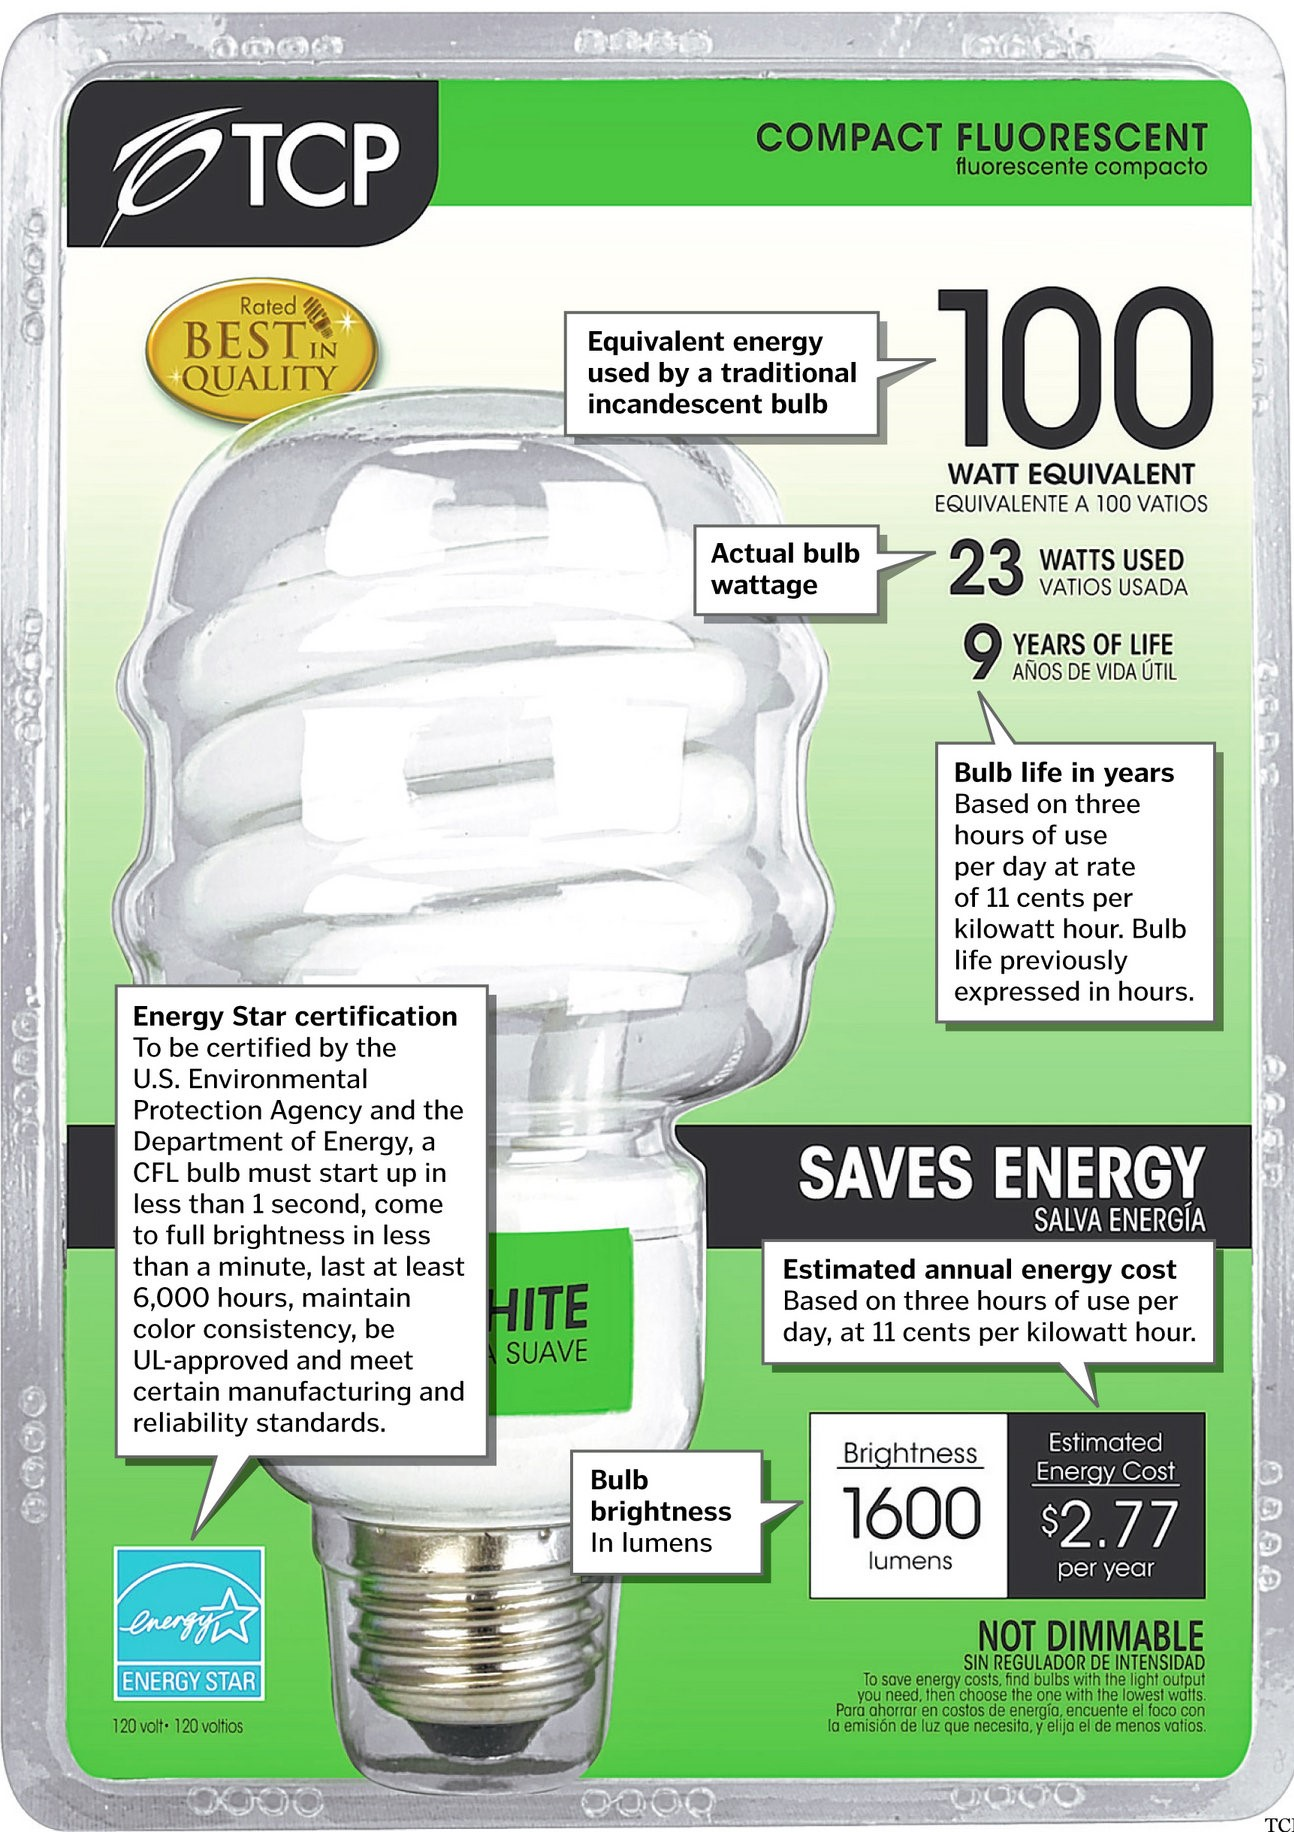
\includegraphics[width=0.5\linewidth]{images/BULB} 

}

\caption{How do we know so much about this unused lightbulb?}\label{fig:unnamed-chunk-3}
\end{figure}

\begin{center}\rule{0.5\linewidth}{0.5pt}\end{center}

\textbf{Question 2:}

An economist wants to forecast the future state of output in the economy. What variables (i.e., leading indicators) should be included in her model? How much confidence should we place in her predictions?

\begin{figure}

{\centering 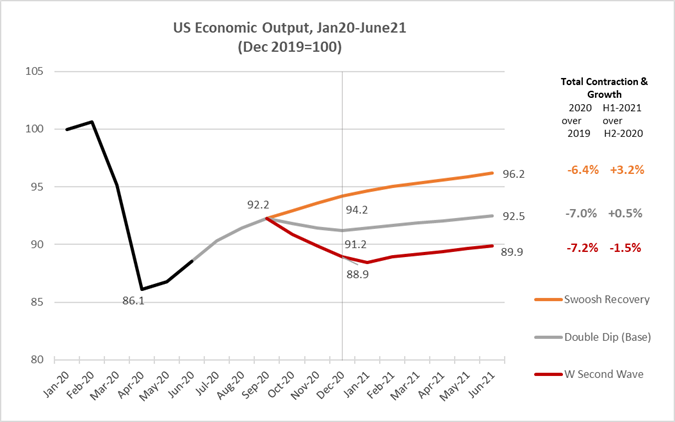
\includegraphics[width=0.8\linewidth]{images/ECONOMIC} 

}

\caption{The Dismal Science}\label{fig:unnamed-chunk-4}
\end{figure}

\begin{center}\rule{0.5\linewidth}{0.5pt}\end{center}

\textbf{Question 3:}

A meteorologist wants to predict the path of a hurricane. How confident can we be in her predicted path of the storm?

\begin{figure}

{\centering 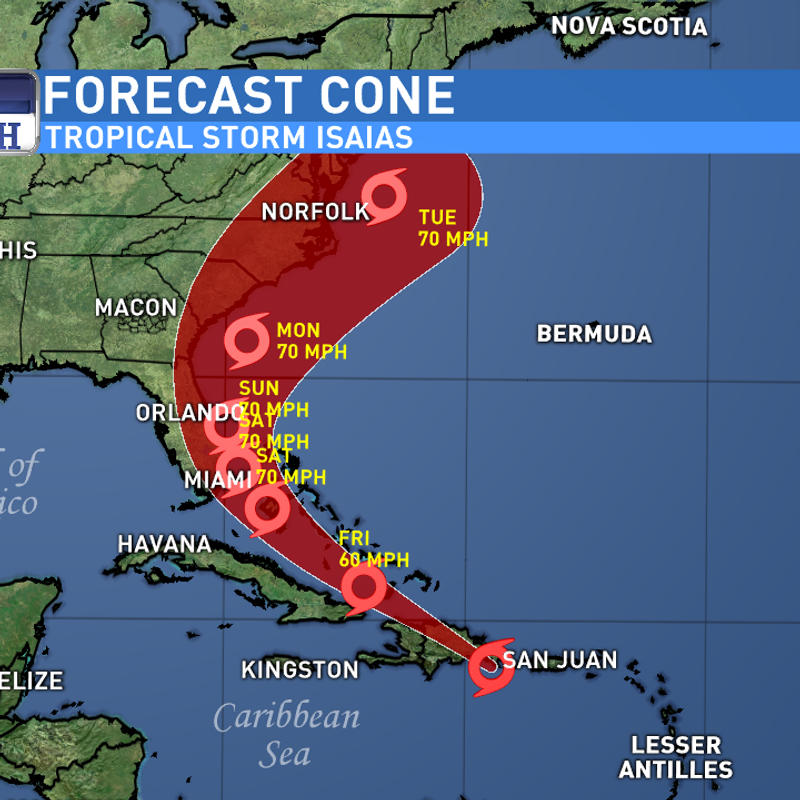
\includegraphics[width=0.7\linewidth]{images/FORECASTCONE} 

}

\caption{The Cone of Uncertainty}\label{fig:unnamed-chunk-5}
\end{figure}

\begin{center}\rule{0.5\linewidth}{0.5pt}\end{center}

These and many more relevant questions can be answered (as best as possible) using \textbf{statistics}.

\begin{quote}
\textbf{Statistics} is the branch of mathematics that transforms data into useful information for decision makers. Statistics are used to summarize data, draw conclusions, make forecasts, and make better sense of the world and the decisions we make within it.
\end{quote}

Statistics is broken into two related branches.

\begin{quote}
\textbf{Descriptive statistics} are used to summarize, analyze, and present data. Since the values of a dataset are in hand (i.e., observable), the descriptive statistics of a dataset are \emph{facts}.
\end{quote}

\begin{quote}
\textbf{Inferential statistics} use the descriptive statistics from the data to draw conclusions about a larger group of observations that at the moment are \emph{impossible} (or too expensive) to observe. Since this larger group of data is not in hand, the inferential statistics that stem from an analysis are \emph{predictions}.
\end{quote}

\begin{center}\rule{0.5\linewidth}{0.5pt}\end{center}

\hypertarget{the-vocabulary-of-statistics}{%
\section{The Vocabulary of Statistics}\label{the-vocabulary-of-statistics}}

\begin{itemize}
\item
  A \textbf{variable} is a characteristic of an item or group that one wishes to analyze.
\item
  \textbf{Data} are the different values of the variable observed and recorded.
\item
  An \textbf{operational definition} establishes a meaningful use of the variable. Simply put, we need to ensure the data sufficiently captures what you want to analyze.
\item
  A \textbf{population} consists of all items you want to draw a conclusion from. The issue with a population is that it is the entire universe of observations that you are interested in, but they can never be fully observed.

  \begin{itemize}
  \item
    Sometimes a population is too costly to collect and analyze. For example, you won't call up every single voter for an election poll.
  \item
    Sometimes a population is impossible to collect because some observations have yet to be determined. For example, the population of end-of-day indices for the S\&P 500 includes every observation that has ever existed as well as every observation \textbf{that has yet to exist}.
  \end{itemize}
\item
  A \textbf{sample} is the portion (i.e., subset) of a population selected for analysis. These are our observations in hand.
\item
  A \textbf{statistic} is a characteristic of a sample. Since we can observe the sample (i.e., our data), these are our descriptive statistics.
\item
  A \textbf{Parameter} is a characteristic of a population. Since we cannot observe the population, the best we can do is draw inferential statistics (or predictions) about them. While the value of a parameter exists, we would have to be omniscient in order to know it. The best we can do is use our sample statistics to construct an \emph{educated guess} of what this value might be.
\end{itemize}

Recall the problem of the wholesaler who has a supply of light bulbs. It would be great if we could state what the \emph{average lifespan} of the light bulbs are, but that would require timing every light bulb until they burn out. This isn't very useful.

The seven terms stated above translate to our light bulb example as follows:

\begin{longtable}[]{@{}ll@{}}
\toprule
\begin{minipage}[b]{(\columnwidth - 1\tabcolsep) * \real{0.60}}\raggedright
Term\strut
\end{minipage} & \begin{minipage}[b]{(\columnwidth - 1\tabcolsep) * \real{0.40}}\raggedright
Our light bulb problem\strut
\end{minipage}\tabularnewline
\midrule
\endhead
\begin{minipage}[t]{(\columnwidth - 1\tabcolsep) * \real{0.60}}\raggedright
Variable\strut
\end{minipage} & \begin{minipage}[t]{(\columnwidth - 1\tabcolsep) * \real{0.40}}\raggedright
The lifespan of a light bulb\strut
\end{minipage}\tabularnewline
\begin{minipage}[t]{(\columnwidth - 1\tabcolsep) * \real{0.60}}\raggedright
Data\strut
\end{minipage} & \begin{minipage}[t]{(\columnwidth - 1\tabcolsep) * \real{0.40}}\raggedright
The light bulbs that you actually plugged in and recorded the time it takes until burnt out\strut
\end{minipage}\tabularnewline
\begin{minipage}[t]{(\columnwidth - 1\tabcolsep) * \real{0.60}}\raggedright
Operational Definition\strut
\end{minipage} & \begin{minipage}[t]{(\columnwidth - 1\tabcolsep) * \real{0.40}}\raggedright
The lifespan \emph{in minutes}\strut
\end{minipage}\tabularnewline
\begin{minipage}[t]{(\columnwidth - 1\tabcolsep) * \real{0.60}}\raggedright
Population\strut
\end{minipage} & \begin{minipage}[t]{(\columnwidth - 1\tabcolsep) * \real{0.40}}\raggedright
The entire group of light bulbs (all 100,000 of them)\strut
\end{minipage}\tabularnewline
\begin{minipage}[t]{(\columnwidth - 1\tabcolsep) * \real{0.60}}\raggedright
Sample\strut
\end{minipage} & \begin{minipage}[t]{(\columnwidth - 1\tabcolsep) * \real{0.40}}\raggedright
The subset of the population selected for analysis. Sometimes referred to as the \emph{data sample}.\strut
\end{minipage}\tabularnewline
\begin{minipage}[t]{(\columnwidth - 1\tabcolsep) * \real{0.60}}\raggedright
Statistic\strut
\end{minipage} & \begin{minipage}[t]{(\columnwidth - 1\tabcolsep) * \real{0.40}}\raggedright
The average lifespan of every light bulb \textbf{in the sample}\strut
\end{minipage}\tabularnewline
\begin{minipage}[t]{(\columnwidth - 1\tabcolsep) * \real{0.60}}\raggedright
Parameter\strut
\end{minipage} & \begin{minipage}[t]{(\columnwidth - 1\tabcolsep) * \real{0.40}}\raggedright
The average lifespan of every light bulb \textbf{in the population}\strut
\end{minipage}\tabularnewline
\bottomrule
\end{longtable}

Inferential statistics allow us to describe the parameter of a population by using the corresponding statistic of a sample. We will \textbf{never} be able to truly know the population parameter, because the information available in the sample is all we got.

How do we know if the sample statistic is a GOOD predictor of the population parameter? The kicker is that since we cannot observe the population, the only thing we can do is try our best to ensure that the characteristics of the sample are the same as the population. This has to do with sample selection - a very important topic that will be addressed soon. First, we start by discussing the descriptive measures of data.

\begin{center}\rule{0.5\linewidth}{0.5pt}\end{center}

\hypertarget{descriptive-measures}{%
\section{Descriptive Measures}\label{descriptive-measures}}

This section summarizes the measures we use to describe data samples.

\begin{itemize}
\item
  \textbf{Central Tendency}: the central value of a data set
\item
  \textbf{Variation}: the dispersion (scattering) around a central value
\item
  \textbf{Shape}: the distribution pattern of the data values
\end{itemize}

These measures will be used repeatedly in our analyses, and will affect how confident we are in our conclusions.

To introduce you to some numerical results in R, we will continue with our light bulb scenario and add some actual data. Suppose we sampled 60 light bulbs from our population, turned them on, and timed each one until it burned out. If we recorded the lifetime of each light bulb, then we have a dataset (or data sample) of 60 observations on the lifetimes of light bulbs. This is what we will be using below.

\begin{center}\rule{0.5\linewidth}{0.5pt}\end{center}

\hypertarget{central-tendency}{%
\subsection{Central Tendency}\label{central-tendency}}

The \textbf{Arithmetic} or \textbf{sample mean} is the average value of a variable within the sample.

\[\bar{X}=\frac{\text{Sum of values}}{\text{Number of observations}}=\frac{1}{n} \sum\limits_{i=1}^n X_i\]

\begin{Shaded}
\begin{Highlighting}[]
\CommentTok{\# the mean of our light bulb sample:}
\CommentTok{\# First we load the data set and this will give us 60 observations of the lifespan of each of our 60 light bulbs in the sample. The variable is called "Lifetime" {-} which can be observed by using the "list" command.}

\FunctionTok{load}\NormalTok{(}\StringTok{"data/Lightbulb.Rdata"}\NormalTok{)}
\FunctionTok{list}\NormalTok{(Lifetime)}
\end{Highlighting}
\end{Shaded}

\begin{verbatim}
## [[1]]
##  [1]  858.9164  797.2652 1013.5366 1064.8195  874.2275  825.1137  897.0879  924.0998  870.0674  966.2095
## [11]  955.1281  977.2073  888.1690  826.6483  776.7479  877.5691  998.7101  892.8178  886.0261  831.7615
## [21] 1082.9650 1034.9549  784.5026  919.2082 1049.1824  923.5767  907.7295  890.3758  856.4240  808.8035
## [31] 1009.7146  890.3709  930.9597  809.9274  919.9381  793.7455  919.9824  948.8593  810.6887  846.9573
## [41]  955.3873  833.2762  892.4969  973.1861  913.7650  928.6057  940.7637  964.4341  914.2733  880.3329
## [51]  831.5395  967.2442 1030.7598  857.5421  889.3689 1094.1440  927.7684  730.9976  918.8359  867.5931
\end{verbatim}

\begin{Shaded}
\begin{Highlighting}[]
\NormalTok{(}\FunctionTok{mean}\NormalTok{(Lifetime))}
\end{Highlighting}
\end{Shaded}

\begin{verbatim}
## [1] 907.5552
\end{verbatim}

The average lifetime of our 60 \((n=60)\) observed light bulbs is 908 hours.

\begin{center}\rule{0.5\linewidth}{0.5pt}\end{center}

The \textbf{median} is the middle value of an ordered data set.

\begin{itemize}
\item
  If there is an odd number of values in a data set, the median is the middle value
\item
  If there an even number, median is the average of the two middle values
\end{itemize}

\begin{Shaded}
\begin{Highlighting}[]
\CommentTok{\# the median of our light bulb sample:}
\NormalTok{(}\FunctionTok{median}\NormalTok{(Lifetime))}
\end{Highlighting}
\end{Shaded}

\begin{verbatim}
## [1] 902.4087
\end{verbatim}

The median lifetime of our 60 observed light bulbs is 902 hours.

\begin{center}\rule{0.5\linewidth}{0.5pt}\end{center}

The \textbf{mode} is the most frequently appearing value in a set of observations. The mode might not exist if there is a set of unique, non-repeating observations.

\begin{Shaded}
\begin{Highlighting}[]
\CommentTok{\# There isn\textquotesingle{}t a built in function for the mode in R... but we can create one.}

\NormalTok{Mode }\OtherTok{\textless{}{-}} \ControlFlowTok{function}\NormalTok{(x) \{}
\NormalTok{  ux }\OtherTok{\textless{}{-}} \FunctionTok{unique}\NormalTok{(x)}
\NormalTok{  ux[}\FunctionTok{which.max}\NormalTok{(}\FunctionTok{tabulate}\NormalTok{(}\FunctionTok{match}\NormalTok{(x, ux)))]}
\NormalTok{\}}

\NormalTok{(}\FunctionTok{Mode}\NormalTok{(Lifetime))}
\end{Highlighting}
\end{Shaded}

\begin{verbatim}
## [1] 858.9164
\end{verbatim}

The most commonly observed lifetime of our 60 observed light bulbs is 859 hours. Note that this doesn't say anything really about how many times this value has been observed, just that it has been observed more than any other value. We will not be using this measure as much as the previous two.

\begin{center}\rule{0.5\linewidth}{0.5pt}\end{center}

\textbf{Percentiles} break the ordered values of a sample into proportions.

\begin{itemize}
\item
  Quartiles split the data into 4 equal parts
\item
  Deciles split the data into 10 equal parts
\item
  In general, the pth percentile is given by: \((p * 100)^{th}=p(n+1)\)
\end{itemize}

A percentile delivers an observed value such that a determined proportion of observations are less than or equal to that value. You can choose any percentile value you wish. For example, the code below calculates the 4th, 40th, and 80th percentiles of our light bulb sample.

\begin{Shaded}
\begin{Highlighting}[]
\CommentTok{\# You can generate any percentile (e.g. the 4th, 40th, and 80th) using the quantile function:}
\NormalTok{(}\FunctionTok{quantile}\NormalTok{(Lifetime,}\FunctionTok{c}\NormalTok{(}\FloatTok{0.04}\NormalTok{, }\FloatTok{0.40}\NormalTok{, }\FloatTok{0.80}\NormalTok{)))}
\end{Highlighting}
\end{Shaded}

\begin{verbatim}
##       4%      40%      80% 
## 787.8301 888.8889 966.4164
\end{verbatim}

This result states that 4\% of our observations are less that 788 hours, 40\% of our observations are less than 889 hours, and 80\% of our observations are less than 966 hours. Note that the median (being the middle-ranked observation) is by default the 50th percentile.

\begin{Shaded}
\begin{Highlighting}[]
\NormalTok{(}\FunctionTok{quantile}\NormalTok{(Lifetime,}\FloatTok{0.50}\NormalTok{))}
\end{Highlighting}
\end{Shaded}

\begin{verbatim}
##      50% 
## 902.4087
\end{verbatim}

\begin{center}\rule{0.5\linewidth}{0.5pt}\end{center}

The main items of central tendency can be laid out in a Five-Number Summary:

\begin{itemize}
\tightlist
\item
  Minimum
\item
  First Quartile (25th percentile)
\item
  Second Quartile (median)
\item
  Third Quartile (75th percentile)
\item
  Maximum
\end{itemize}

\begin{Shaded}
\begin{Highlighting}[]
\FunctionTok{summary}\NormalTok{(Lifetime)}
\end{Highlighting}
\end{Shaded}

\begin{verbatim}
##    Min. 1st Qu.  Median    Mean 3rd Qu.    Max. 
##   731.0   857.3   902.4   907.6   955.2  1094.1
\end{verbatim}

\begin{center}\rule{0.5\linewidth}{0.5pt}\end{center}

\hypertarget{variation}{%
\subsection{Variation}\label{variation}}

The \textbf{sample variance} measures the average (squared) amount of dispersion each individual observation has around the sample mean. This is a very important measure in statistics, so take some time to understand exactly what this equation is calculating. In particular, \(X\) is a variable and \(X_i\) is an arbitrary single observation from that group of data. Once the mean \((\bar{X})\) is calculated, \(X_i - \bar{X}\) is the difference between a single observation of X and the overall mean of X. Sometimes this difference is negative \((X_i < \bar{X})\) and sometimes this difference is positive \(X_i > \bar{X}\) - which is why we need to square these differences before adding them all up. Nonetheless, once we obtain the average value of these differences, we get a sense of the amount of dispersion these individual observations are scattered around the sample average. If this value was zero, then \emph{every} observation of \(X\) is equal to \(\bar{X}\). The greater the value is from zero, the greater the average dispersion of individual values around the mean.

\[S^2=\frac{1}{n-1}\sum\limits_{i=1}^n(X_i-\bar{X})^2\]

The \textbf{sample standard deviation} is the square-root of the sample variance and measures the average amount of dispersion in the same units as the mean. This essentially is done to back-out the fact that we had to square the differences of \(X_i - \bar{X}\), so the variance is technically denoted in \emph{squared units}.

\[S=\sqrt{S^2}\]

\begin{Shaded}
\begin{Highlighting}[]
\NormalTok{(}\FunctionTok{var}\NormalTok{(Lifetime))}
\end{Highlighting}
\end{Shaded}

\begin{verbatim}
## [1] 6235.852
\end{verbatim}

\begin{Shaded}
\begin{Highlighting}[]
\NormalTok{(}\FunctionTok{sd}\NormalTok{(Lifetime))}
\end{Highlighting}
\end{Shaded}

\begin{verbatim}
## [1] 78.96741
\end{verbatim}

The variance of our sample of light bulb lifetimes is 6236 squared-hours. After taking the square root of this number, we can conclude that the standard deviation of our sample is 79 hours. Is this standard deviation big or small? The answer to this comes when we get to statistical inference.

\hypertarget{discussion}{%
\subsubsection*{Discussion}\label{discussion}}
\addcontentsline{toc}{subsubsection}{Discussion}

\begin{itemize}
\item
  The term \((X_i-\bar{X})\) is squared because individual observations are either above or below the mean by design. If you don't square the terms (making the negative numbers positive) then they will sum to zero by design.
\item
  The term \((n-1)\) appears in the denominator because this is a \emph{sample} variance and not a \emph{population} variance. In a population variance equation, \((n-1)\) gets replaced with \(n\) because we know the population mean. Since we had to estimate the population mean (i.e., used the sample mean), we had to deduct one \textbf{degree of freedom}. We will talk more about degrees of freedom later, but the rule of thumb is that we deduct a degree of freedom every time we build a sample statistic (like sample variance) using another sample statistic (like sample mean).
\end{itemize}

\begin{center}\rule{0.5\linewidth}{0.5pt}\end{center}

The \textbf{coefficient of variation} is a relative measure which denotes the amount of scatter in the data relative to the mean.

The coefficient of variation is useful when comparing data on variables measured in different units or scales (because the CV reduces everything to percentages).

\[CV=\frac{S}{\bar{X}}*100\%\]

Take for example the Gross Domestic Product (i.e., output) for the states of California and Delaware.

\begin{Shaded}
\begin{Highlighting}[]
\FunctionTok{library}\NormalTok{(readxl)}
\NormalTok{CARGSP }\OtherTok{\textless{}{-}} \FunctionTok{read\_excel}\NormalTok{(}\StringTok{"data/CARGSP.xls"}\NormalTok{)}
\NormalTok{DENGSP }\OtherTok{\textless{}{-}} \FunctionTok{read\_excel}\NormalTok{(}\StringTok{"data/DENGSP.xls"}\NormalTok{)}

\NormalTok{CGDP }\OtherTok{\textless{}{-}}\NormalTok{ CARGSP}\SpecialCharTok{$}\NormalTok{CGDP}
\NormalTok{DGDP }\OtherTok{\textless{}{-}}\NormalTok{ DENGSP}\SpecialCharTok{$}\NormalTok{DGDP}

\NormalTok{(}\FunctionTok{mean}\NormalTok{(CGDP))}
\end{Highlighting}
\end{Shaded}

\begin{verbatim}
## [1] 2094764
\end{verbatim}

\begin{Shaded}
\begin{Highlighting}[]
\NormalTok{(}\FunctionTok{sd}\NormalTok{(CGDP))}
\end{Highlighting}
\end{Shaded}

\begin{verbatim}
## [1] 397103.9
\end{verbatim}

\begin{Shaded}
\begin{Highlighting}[]
\NormalTok{(}\FunctionTok{mean}\NormalTok{(DGDP))}
\end{Highlighting}
\end{Shaded}

\begin{verbatim}
## [1] 56996.58
\end{verbatim}

\begin{Shaded}
\begin{Highlighting}[]
\NormalTok{(}\FunctionTok{sd}\NormalTok{(DGDP))}
\end{Highlighting}
\end{Shaded}

\begin{verbatim}
## [1] 12395.78
\end{verbatim}

A quick analysis of the real annual output observations from these two states between the years 1997 and 2020 suggest that the average annual output of California is 2,094,764 million dollars (with a standard deviation of 397,104 million) and that of Delaware is 56,997 million dollars (with a standard deviation of 12,396 million). These two states have lots of differences between them, and it is difficult to tell which state has more volatility in their output.

If we construct coefficients of variation:

\begin{Shaded}
\begin{Highlighting}[]
\NormalTok{(}\FunctionTok{sd}\NormalTok{(CGDP)}\SpecialCharTok{/}\FunctionTok{mean}\NormalTok{(CGDP))}\SpecialCharTok{*}\DecValTok{100}
\end{Highlighting}
\end{Shaded}

\begin{verbatim}
## [1] 18.95698
\end{verbatim}

\begin{Shaded}
\begin{Highlighting}[]
\NormalTok{(}\FunctionTok{sd}\NormalTok{(DGDP)}\SpecialCharTok{/}\FunctionTok{mean}\NormalTok{(DGDP))}\SpecialCharTok{*}\DecValTok{100}
\end{Highlighting}
\end{Shaded}

\begin{verbatim}
## [1] 21.74828
\end{verbatim}

We can now conclude that Delaware's standard deviation of output is almost 22\% that of its' average output, while California's standard deviation is 19\%. This would suggest that Delaware has the more volatile output, relatively speaking.

\begin{center}\rule{0.5\linewidth}{0.5pt}\end{center}

\hypertarget{measures-of-shape}{%
\subsection{Measures of shape}\label{measures-of-shape}}

Comparing the mean and median of a sample will inform us of the skewness of the distribution.

\begin{itemize}
\tightlist
\item
  mean = median: a \emph{symmetric} or \emph{zero-skewed} distribution.
\end{itemize}

\begin{center}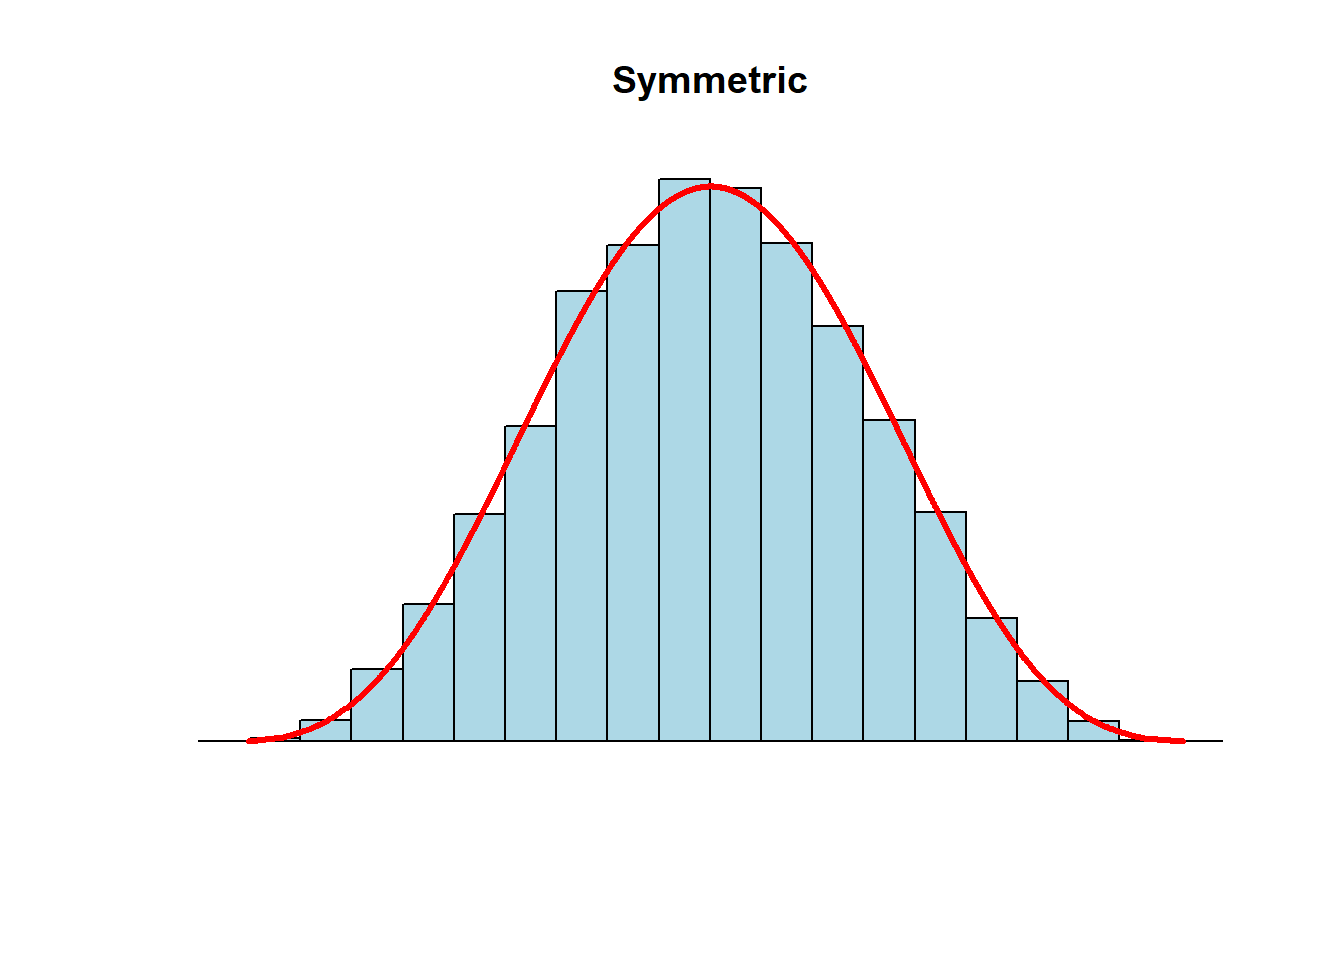
\includegraphics{MBA8350book_files/figure-latex/unnamed-chunk-15-1} \end{center}

\begin{itemize}
\tightlist
\item
  mean \textgreater{} median: a \emph{positive-skewed} or \emph{right-skewed} distribution

  \begin{itemize}
  \tightlist
  \item
    the right-tail is pulled in the positive direction
  \end{itemize}
\end{itemize}

\begin{center}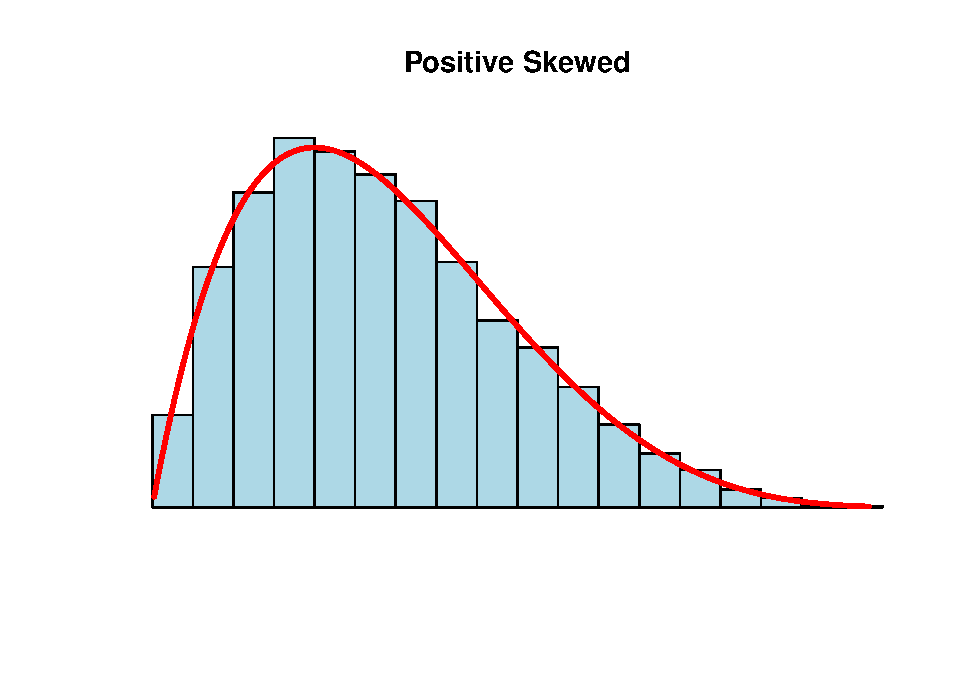
\includegraphics{MBA8350book_files/figure-latex/unnamed-chunk-16-1} \end{center}

\begin{itemize}
\tightlist
\item
  mean \textless{} median: a \emph{negative-skewed} or a \emph{left-skewed} distribution

  \begin{itemize}
  \tightlist
  \item
    the left-tail is pulled in the negative direction
  \end{itemize}
\end{itemize}

\begin{center}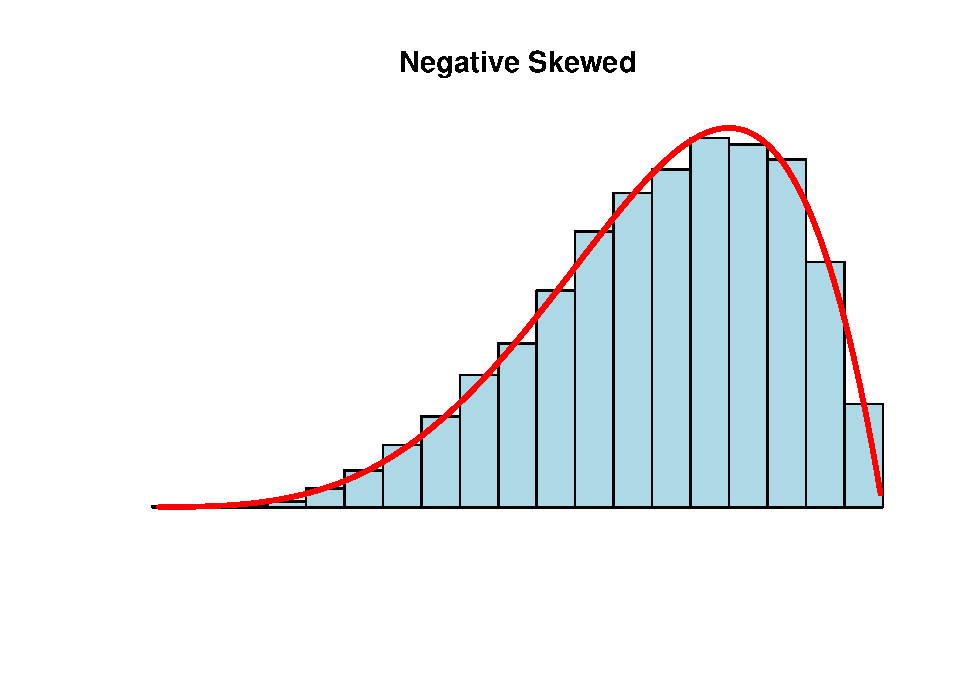
\includegraphics{MBA8350book_files/figure-latex/unnamed-chunk-17-1} \end{center}

The degree of skewness is indicative of outliers (extreme high or low values) which change the shape of a distribution.

\hypertarget{covariance-and-correlation}{%
\subsection{Covariance and Correlation}\label{covariance-and-correlation}}

While we won't be examining relationships between different variables until later on in the course, we can easily calculate and visualize these relationships.

The \textbf{covariance} measures the strength of the relationship between two variables. This measure is similar to a variance, but it can be either positive or negative depending on how the two variables move in relation to each other.

\[cov(X,Y)=\frac{1}{n-1}\sum\limits_{i=1}^n(X_i-\bar{X})(Y_i-\bar{Y})\]

The \textbf{coefficient of correlation} transforms the covariance into a relative measure

\[corr(X,Y)=\frac{cov(X,Y)}{S_{X}S_{Y}}\]
The correlation transformed the covariance relationship into a measure between -1 and 1

\begin{itemize}
\item
  \(corr(X,Y)=0\): There is no relationship between \(X\) and \(Y\)
\item
  \(corr(X,Y)>0\): There is a positive relationship between \(X\) and \(Y\) - meaning that the two variables tend to move in the same direction
\item
  \(corr(X,Y)<0\): There is a negative relationship between \(X\) and \(Y\) - meaning that the two variables tend to move in the opposite direction
\end{itemize}

\hypertarget{extended-example}{%
\subsubsection*{Extended Example:}\label{extended-example}}
\addcontentsline{toc}{subsubsection}{Extended Example:}

This chapter concludes with a summary of all of the descriptive measures we discussed. Consider a dataset that is internal to R (called mtcars) that contains characteristics of 32 different automobiles. We will focus on two variables: the average miles per gallon (mpg) and the weight of the car (in thousands of pounds).

\begin{Shaded}
\begin{Highlighting}[]
\NormalTok{car }\OtherTok{\textless{}{-}}\NormalTok{ mtcars }\CommentTok{\# This loads the dataset and calls it car}

\CommentTok{\# Lets examine mpg first:}
\FunctionTok{summary}\NormalTok{(car}\SpecialCharTok{$}\NormalTok{mpg)}
\end{Highlighting}
\end{Shaded}

\begin{verbatim}
##    Min. 1st Qu.  Median    Mean 3rd Qu.    Max. 
##   10.40   15.43   19.20   20.09   22.80   33.90
\end{verbatim}

\begin{Shaded}
\begin{Highlighting}[]
\FunctionTok{hist}\NormalTok{(car}\SpecialCharTok{$}\NormalTok{mpg,}\DecValTok{20}\NormalTok{,}\AttributeTok{col =} \StringTok{"yellow"}\NormalTok{)}
\end{Highlighting}
\end{Shaded}

\begin{center}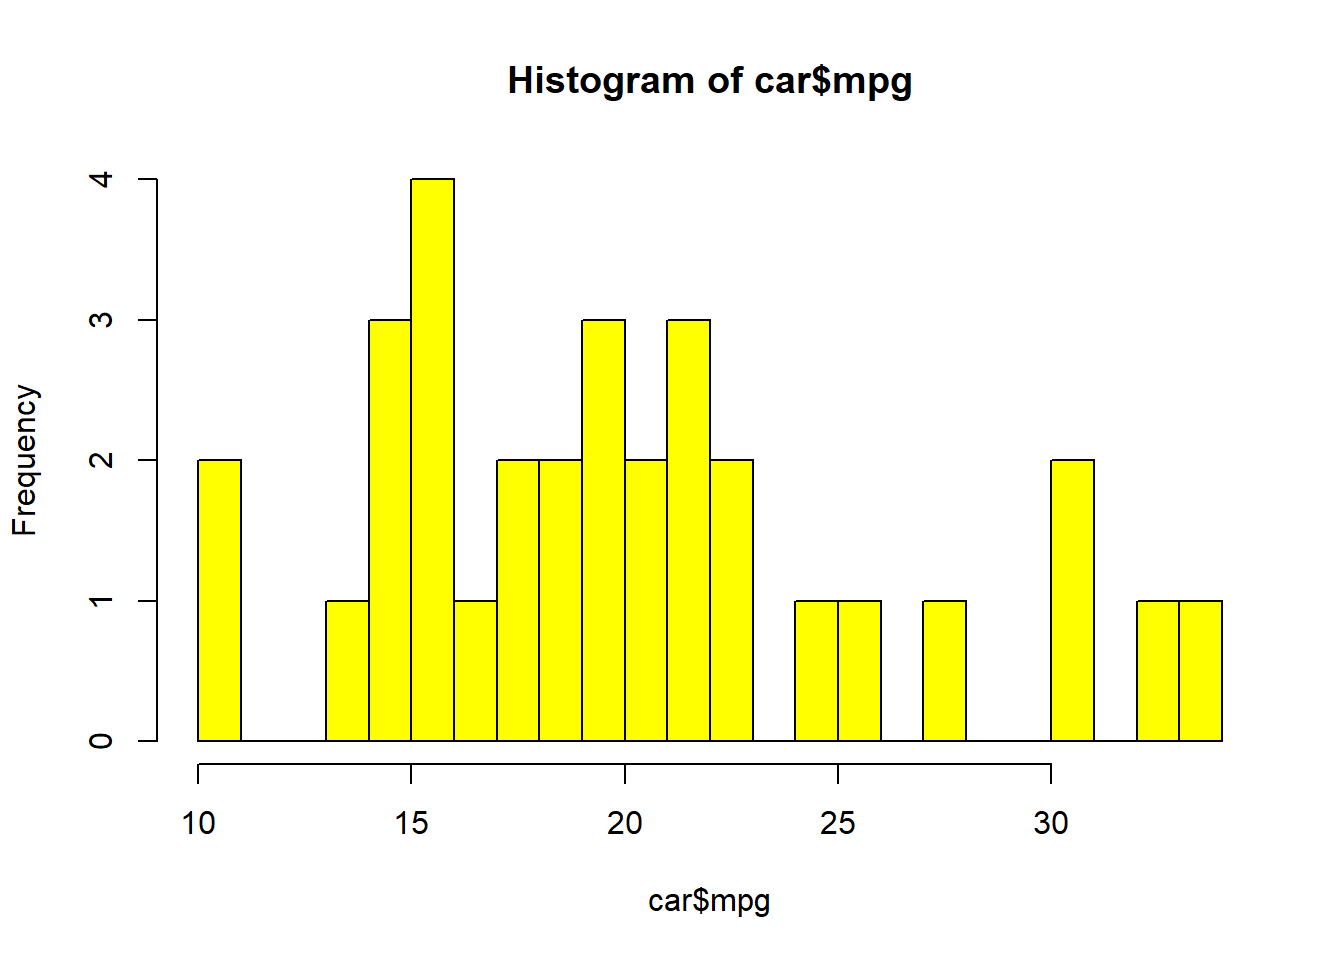
\includegraphics{MBA8350book_files/figure-latex/unnamed-chunk-18-1} \end{center}

\begin{Shaded}
\begin{Highlighting}[]
\CommentTok{\# Variance:}
\NormalTok{(}\FunctionTok{var}\NormalTok{(car}\SpecialCharTok{$}\NormalTok{mpg))}
\end{Highlighting}
\end{Shaded}

\begin{verbatim}
## [1] 36.3241
\end{verbatim}

\begin{Shaded}
\begin{Highlighting}[]
\CommentTok{\# Standard deviation:}
\NormalTok{(}\FunctionTok{sd}\NormalTok{(car}\SpecialCharTok{$}\NormalTok{mpg))}
\end{Highlighting}
\end{Shaded}

\begin{verbatim}
## [1] 6.026948
\end{verbatim}

The above analysis indicates the following:

\begin{itemize}
\item
  The sample average MPG in the sample is 20.09, while the median in 19.20. This indicates that there is a slight positive skew to the distribution of observations.
\item
  The lowest MPG is 10.4 while the highest is 33.90.
\item
  The first quartile is 15.43 while the third is 22.80. This delivers the \emph{inter-quartile range} (the middle 50\% of the distribution)
\item
  The standard deviation is 6.03 which delivers a 30 percent coefficient of correlation.
\end{itemize}

\begin{Shaded}
\begin{Highlighting}[]
\DocumentationTok{\#\# Lets now examine weight:}
\FunctionTok{summary}\NormalTok{(car}\SpecialCharTok{$}\NormalTok{wt)}
\end{Highlighting}
\end{Shaded}

\begin{verbatim}
##    Min. 1st Qu.  Median    Mean 3rd Qu.    Max. 
##   1.513   2.581   3.325   3.217   3.610   5.424
\end{verbatim}

\begin{Shaded}
\begin{Highlighting}[]
\FunctionTok{hist}\NormalTok{(car}\SpecialCharTok{$}\NormalTok{wt,}\DecValTok{20}\NormalTok{,}\AttributeTok{col =} \StringTok{"pink"}\NormalTok{)}
\end{Highlighting}
\end{Shaded}

\begin{center}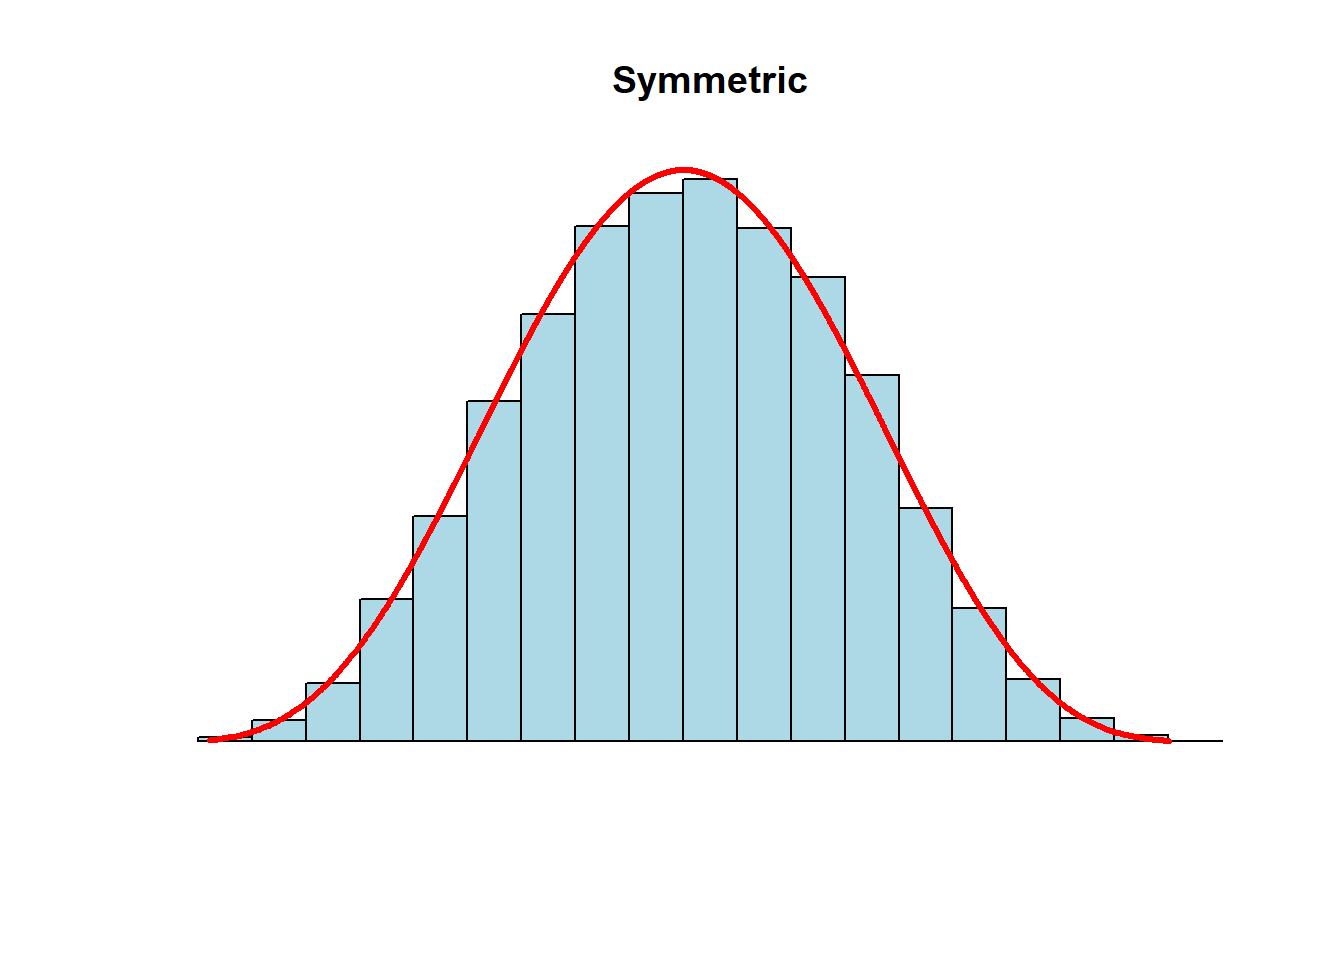
\includegraphics{MBA8350book_files/figure-latex/unnamed-chunk-19-1} \end{center}

\begin{Shaded}
\begin{Highlighting}[]
\CommentTok{\# Variance:}
\NormalTok{(}\FunctionTok{var}\NormalTok{(car}\SpecialCharTok{$}\NormalTok{wt))}
\end{Highlighting}
\end{Shaded}

\begin{verbatim}
## [1] 0.957379
\end{verbatim}

\begin{Shaded}
\begin{Highlighting}[]
\CommentTok{\# Standard deviation:}
\NormalTok{(}\FunctionTok{sd}\NormalTok{(car}\SpecialCharTok{$}\NormalTok{wt))}
\end{Highlighting}
\end{Shaded}

\begin{verbatim}
## [1] 0.9784574
\end{verbatim}

The above analysis indicates the following:

\begin{itemize}
\item
  The sample average weight in the sample is 3.22 thousand pounds, while the median in 3.33. This indicates that there is a slight negative skew to the distribution of observations.
\item
  The lowest weight is 1.51 while the highest is 5.42.
\item
  The first quartile is 2.58 while the third is 3.61.
\item
  The standard deviation is 0.99 which also delivers a 30 percent coefficient of correlation.
\end{itemize}

\begin{Shaded}
\begin{Highlighting}[]
\CommentTok{\# We can now look at the relation between mpg and weight}

\NormalTok{(}\FunctionTok{cov}\NormalTok{(car}\SpecialCharTok{$}\NormalTok{mpg,car}\SpecialCharTok{$}\NormalTok{wt))}
\end{Highlighting}
\end{Shaded}

\begin{verbatim}
## [1] -5.116685
\end{verbatim}

\begin{Shaded}
\begin{Highlighting}[]
\NormalTok{(}\FunctionTok{cor}\NormalTok{(car}\SpecialCharTok{$}\NormalTok{mpg,car}\SpecialCharTok{$}\NormalTok{wt))}
\end{Highlighting}
\end{Shaded}

\begin{verbatim}
## [1] -0.8676594
\end{verbatim}

\begin{Shaded}
\begin{Highlighting}[]
\FunctionTok{plot}\NormalTok{(car}\SpecialCharTok{$}\NormalTok{mpg,car}\SpecialCharTok{$}\NormalTok{wt,}
     \AttributeTok{xlab =} \StringTok{"Miles per gallon"}\NormalTok{,}
     \AttributeTok{ylab =} \StringTok{"Weight of car"}\NormalTok{,}
     \AttributeTok{main =} \StringTok{"A Scatter plot"}\NormalTok{,}
     \AttributeTok{col =} \StringTok{"cyan"}\NormalTok{)}
\end{Highlighting}
\end{Shaded}

\begin{center}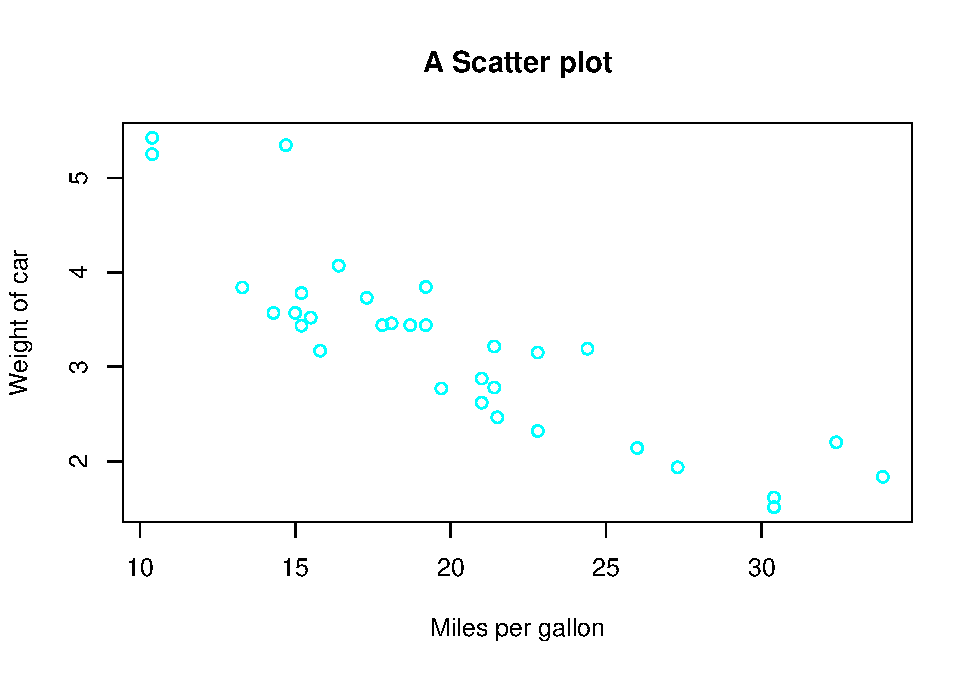
\includegraphics{MBA8350book_files/figure-latex/unnamed-chunk-20-1} \end{center}

The negative correlation as well as the obviously negative relationship in the scatter-plot between the weight of a car and its miles per gallon should make intuitive sense - heavy cars are less efficient.

\hypertarget{the-punchline}{%
\subsubsection*{The Punchline}\label{the-punchline}}
\addcontentsline{toc}{subsubsection}{The Punchline}

Suppose we want to learn about a relationship between a car's weight and its fuel efficiency. Our sample is 32 automobiles, but our population is EVERY automobile (EVER). We would like to say something about the population mean Weight and MPG.

How does the sample variance(s) give us confidence on making statements about the population mean when we're only given the sample? That's where inferential statistics comes in. Before we get into that, we will dig into elements of collecting data (upon which our descriptive statistics are based on) and using R (with which we will use to calculate our descriptive statistics using our collected data).

\hypertarget{Data}{%
\chapter{Data Collection and Sampling}\label{Data}}

Always remember the ultimate goal of inferential statistics: We want to say something important about the characteristics (parameters) of a population without ever observing the entire population. Therefore, the best thing we can do is to draw a sample (i.e., subset) from the population and use it to calculate characteristics (statistics) of a sample and draw inference on the population parameters.

The reason why we can say something about a population parameter of interest solely by looking at the statistics from a sample is because we are under the assumption that \emph{the sample has the same characteristics of the population}. In other words, we say that the sample average is a good guess for the population average, the sample standard deviation is a good guess for the population standard deviation, etc. This is not an assumption that is simply made by wishful thinking. In fact, there is an entire field of statistics devoted to proper \emph{sample selection}. We won't spend a lot of time on this very important matter, but we will discuss a few sampling methods so you can rest assured that our crucial assumption of similar sample and population characteristics has a reasonable chance of holding.

\begin{center}\rule{0.5\linewidth}{0.5pt}\end{center}

\hypertarget{sampling-distributions}{%
\section{Sampling Distributions}\label{sampling-distributions}}

Recall that a \textbf{sample} is the subset of a \textbf{population} selected for analysis.

We are forced to analyze a sample rather than a population because:

\begin{enumerate}
\def\labelenumi{\arabic{enumi}.}
\item
  selecting a sample is less time-consuming than selecting the population
\item
  selecting a sample is less costly
\item
  the resulting analysis is less cumbersome and more practical
\item
  sometimes obtaining the sample is \emph{impossible}! So the sample is the best we can do.
\end{enumerate}

When making statements on the population parameters using the sample statistics, we are drawing \textbf{statistical inference}. In order for this inference to be reasonable, we must assume that the characteristics of the sample (i.e., the sample statistics) are reasonably close to the characteristics of the population (i.e., the population parameters). The problem with this assumption is that since we will never see the population, we will never be able to verify if the statistics are reasonably close to the parameters. This chapter discusses several different methods of drawing a sample from a population, as well as their pros and cons. The bottom line is that all of these methods attempt to get a sample to be the best possible subset of the population.

Failing to obtain a sample with the same characteristics as the population can fatally flaw a statistical analysis. If the sample statistics are not close to the population parameters, you are potentially over-representing and/or under-representing important aspects of the population. When the sample statistics do not coincide with the population parameters, then the statistics are said to be \emph{biased}. When this bias stems from a faulty sample, then this is called \textbf{sampling bias}.

\hypertarget{sampling-bias---two-examples}{%
\section{Sampling Bias - two examples}\label{sampling-bias---two-examples}}

There are quite a few glaring examples of sampling bias in history. One of them has to do with a rather famous photo:

\hypertarget{dewey-defeats-truman}{%
\subsection{Dewey Defeats Truman?}\label{dewey-defeats-truman}}

\begin{figure}

{\centering 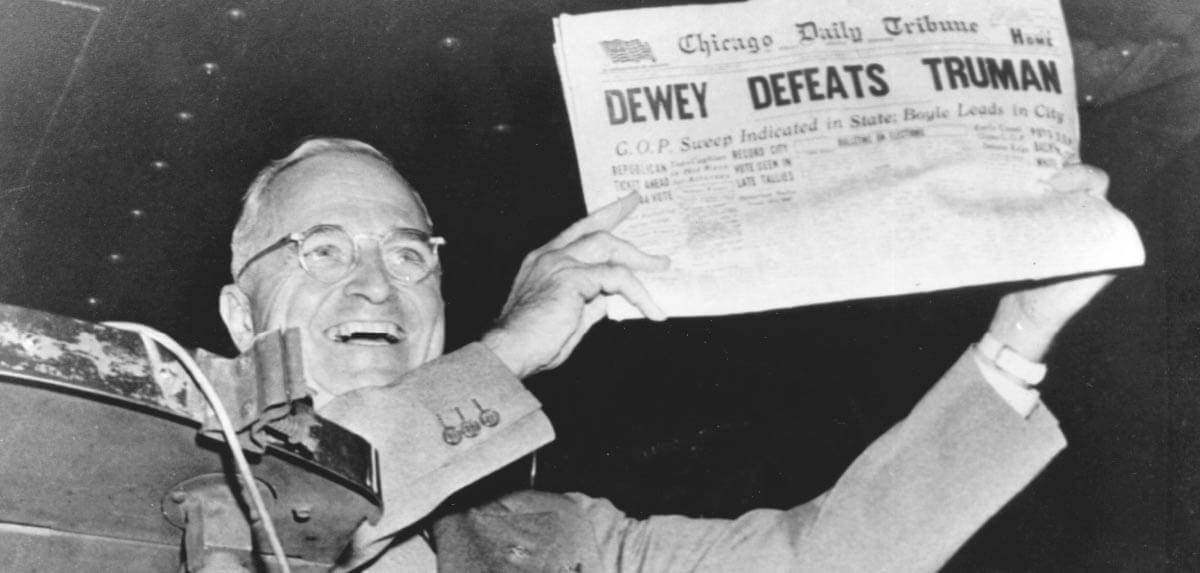
\includegraphics[width=0.5\linewidth]{images/timeline-truman-second-term} 

}

\caption{Dewey Defeats Truman? (1948)}\label{fig:unnamed-chunk-22}
\end{figure}

After defeating Thomas Dewey with a comfortable margin of 303 electoral college votes to Dewey's 189, President Harry Truman holds up a Chicago Daily Tribune stating the exact opposite. While the Truman Library would like to think that this iconic photo is an example of tenacity, perseverance, self-confidence, and success - it's actually a result of \emph{sampling bias}.

The reporting error stems from the fact that the newspaper conducted a poll using phone numbers obtained from a list of vehicle registrations. Most people didn't have phones in 1948, and the people that were being polled had both phones and automobiles. This skewed the sample distribution to wealthy, white, males - which was obviously not sharing similar views with the overall voting population.

\hypertarget{section-1}{%
\subsection{98.6?}\label{section-1}}

Everybody knows the following \emph{fact} about their body\ldots{}

\begin{quote}
The average human body temperature is 98.6 degrees F (37 degrees C).
\end{quote}

Is it really? To put this issue in the context of our terminology, the \emph{average human body temperature} is a population parameter. The population here is every human that has ever lived and ever will live (i.e., an unobtainable sample). This average is actually a sample average obtained by a German physician in 1851 - a time believed by many current physicians to be one where many suffered from chronic infectious diseases resulting in inflammation and mild fevers. Current studies are suggesting the average human body temperature is more like one degree lower than previously thought.

Now to be clear, there is a bit of a semantic argument about this last example. Some empiricists do not call this necessarily a sampling bias issue in 1851, because if a large portion of the population did regularly suffer from mild fevers then the sample was an accurate subset of the population at the time. Of course, if one is saying that the 1851 estimate of 98.6 degrees F is a representation of the \emph{current} population - then that can be regarded as sampling bias.

\hypertarget{sampling-methods}{%
\section{Sampling Methods}\label{sampling-methods}}

The sampling process begins by defining the \textbf{frame} - a listing of items that make up the population. A frame could be population lists, maps, directories, etc. For our Truman example above, the frame was incorrectly chosen to be a list of registered vehicle owners (so the poll was doomed from the start).

A sample is drawn from a frame. The sample could be a \textbf{nonprobability sample} or a \textbf{probability sample}. The items in a nonprobability sample are selected without knowing their probabilities of selection. This is usually done out of convenience (e.g., all voluntary responses to a survey or selecting the top or bottom of a frame). While these samples are quick, convenient, \& inexpensive, they most likely suffer from selection bias. We can perform (albeit, incorrectly) statistical analyses on these samples, but we are going to restrict attention to probability samples which are selected based on known probabilities.

\hypertarget{simple-random-sampling}{%
\subsection{Simple random sampling}\label{simple-random-sampling}}

\begin{figure}

{\centering 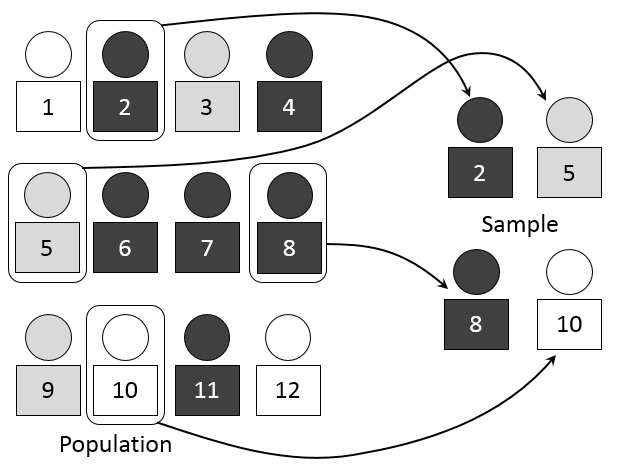
\includegraphics[width=0.5\linewidth]{images/random} 

}

\caption{Simple Random Sampling}\label{fig:unnamed-chunk-23}
\end{figure}

In a \textbf{simple random sample}, every item in a frame has an equal chance of being selected.

The chance (or probability) of being selected depends on if you're selecting\ldots{}

\begin{itemize}
\tightlist
\item
  With replacement (1/N chance for all)
\item
  Without replacement (1/N, 1/(N-1), 1/(N-2), \ldots)
\end{itemize}

Examples of simple random sampling methods:

\begin{itemize}
\tightlist
\item
  Fishbowl methods
\item
  random number indexing
\end{itemize}

\textbf{Advantages:}

\begin{itemize}
\item
  Simple random sampling is associated with the minimum amount of sampling bias compared to other sampling methods.
\item
  If the sample frame is available, selecting a random sample is very easy.
\end{itemize}

\textbf{Disadvantages:}

\begin{itemize}
\item
  Simple random sampling requires a list of all potential respondents (sampling frame) to be available beforehand - which can be costly.
\item
  The necessity to have a large sample size (i.e., lots of observations) can be a major disadvantage in practical levels
\end{itemize}

\hypertarget{systematic-sampling}{%
\subsection{Systematic Sampling}\label{systematic-sampling}}

\begin{figure}

{\centering 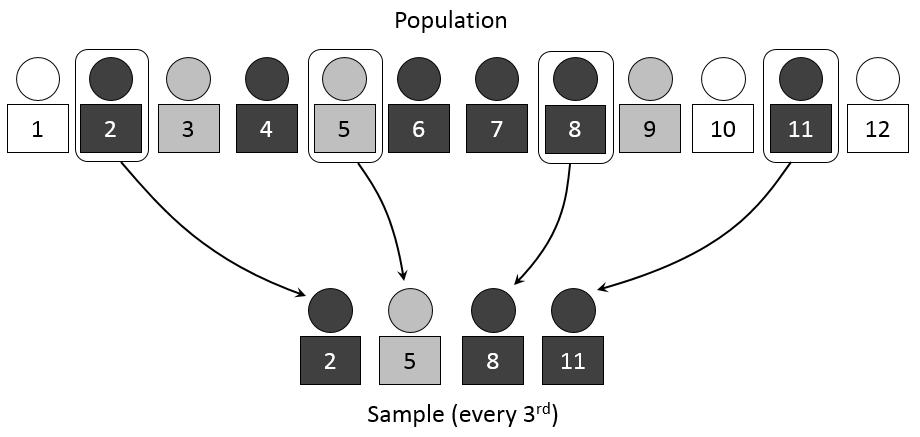
\includegraphics[width=0.7\linewidth]{images/Systematic} 

}

\caption{Systematic Sampling}\label{fig:unnamed-chunk-24}
\end{figure}

A systematic sample begins with partitioning the N items in a frame into n groups of k items

\[k=\frac{N}{n}\]

\begin{itemize}
\item
  randomly select a number from 1 through k
\item
  select the kth member from each of the n groups
\end{itemize}

For example: Suppose you want a sample n=40 out of N=800.

\begin{itemize}
\item
  Divide the population into k=20 groups.
\item
  Select a number from 1-20 (e.g.~8)
\item
  Sample becomes items 8,28,48,68,88,\ldots{}
\end{itemize}

\textbf{Advantages}

\begin{itemize}
\item
  it will approximate the results of simple random sampling
\item
  it is cost and time efficient
\end{itemize}

\textbf{Disadvantages}

\begin{itemize}
\item
  it can be applied only if the complete list of a population is available
\item
  the sample will be biased if there are periodic patterns in the frame
\end{itemize}

\hypertarget{stratified-sampling}{%
\subsection{Stratified Sampling}\label{stratified-sampling}}

\begin{figure}

{\centering 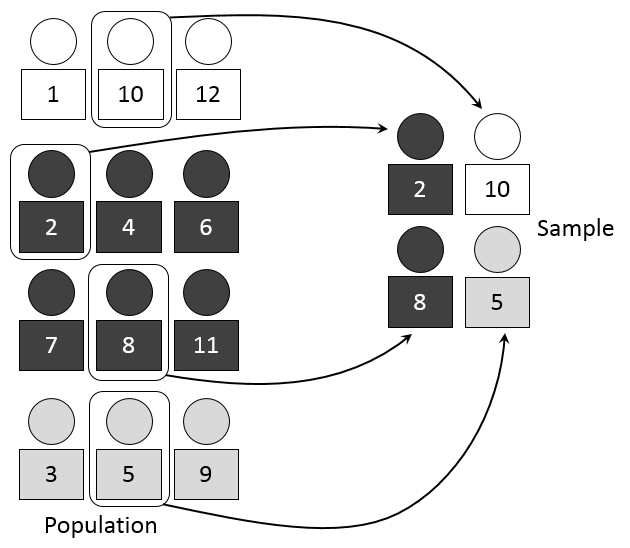
\includegraphics[width=0.5\linewidth]{images/Stratified} 

}

\caption{Stratified Sampling}\label{fig:unnamed-chunk-25}
\end{figure}

A stratified sample divides the N items in the frame into important sub-populations (strata)

\begin{itemize}
\tightlist
\item
  Each strata groups items according to some shared characteristic (gender, education, etc.)
\end{itemize}

Once these strata are constructed. A researcher selects a simple random sample from each strata and combines.

\textbf{Advantages}

\begin{itemize}
\item
  it is superior to simple random sampling because it reduces sampling error and ensures a greater level of representation
\item
  ensures adequate representation of all subgroups
\item
  when there is homogeneity within strata and heterogeneity between strata, the estimates can be as precise (or even more precise) as with the use of simple random sampling
\end{itemize}

\textbf{Disadvantages}

\begin{itemize}
\item
  requires the knowledge of strata membership
\item
  process may take longer and prove to be more expensive due to the extra stage in the sampling procedure
\end{itemize}

\hypertarget{cluster-sampling}{%
\subsection{Cluster Sampling}\label{cluster-sampling}}

\begin{figure}

{\centering 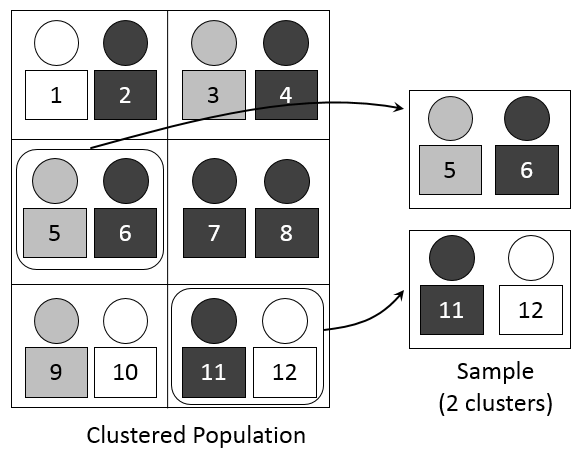
\includegraphics[width=0.5\linewidth]{images/Cluster} 

}

\caption{Cluster Sampling}\label{fig:unnamed-chunk-26}
\end{figure}

\textbf{Cluster Sampling} occurs when you break the sample frame into specific groups (i.e., clusters) and then randomly select several clusters as your sample. An example of this method is the consumer price index (CPI) which is a measure of inflation calculated by the Bureau of Labor Statistics in the U.S. (US BLS). When trying to estimate the overall change in a \emph{basket} of consumption goods across the US, the BLS breaks the US into metropolitan statistical areas (MSAs) and treats each one as a cluster. The BLS then goes and prices the various goods in the clusters selected for analysis.

\textbf{Advantages:}

\begin{itemize}
\item
  the most time-efficient and cost-efficient probability design for large geographical areas
\item
  easy to use
\item
  larger sample size can be used due to increased level of accessibility of perspective sample group members
\end{itemize}

\textbf{Disadvantages}

\begin{itemize}
\item
  requires group-level information to be known
\item
  commonly has higher sampling error than other sampling techniques
\item
  may fail to reflect the diversity in the sampling frame
\end{itemize}

\begin{center}\rule{0.5\linewidth}{0.5pt}\end{center}

\hypertarget{sampling-in-practice}{%
\section{Sampling in Practice}\label{sampling-in-practice}}

The sampling methods above deal with situations in which the population is hypothetically obtainable, but it is not feasible due to time or resource constraints. For example, a company could run a concrete election poll by calling up \emph{every single registered voter} (the population), but that would cost too much and take too long. What happens in the situation where the population is unobtainable, meaning that at any point in time there will be some obtainable portion of the population because it hasn't occurred yet. For example, if I wanted to analyze US unemployment rates, I couldn't possibly consider \emph{future} rates that haven't been observed yet. In situation like these, one must take time to consider exactly what population you want to draw inferences from and draw their sample accordingly.

A quick example of data sampling in my own research is as follows. Some of my research deals with how bank lending responds to changes in the stance of monetary policy.\footnote{Dave, Chetan, Scott J. Dressler, and Lei Zhang, (2013). The bank lending channel: a FAVAR analysis. \emph{Journal of Money, Credit, and Banking} 45(8). 1705-1720.} Since bank lending data is coming in daily, it is clear that the entire population is unobtainable. However, selecting a sample is not simply \emph{collect as many observations as possible} because we must be clear about what population we want to actually talk about. In my example, I want to talk about how bank lending responds to monetary policy shocks \emph{in normal times}. This means that observations in the sample cannot be impacted by episodes where monetary policy differed from what is currently considered normal. This restricts my sample to be after World War 2 and before episodes of unconventional monetary policy (i.e., anything post-2007).

What happens if characteristics of the population potentially changes? That's easy - you repeat the analysis with an updated sample and acknowledge that you are drawing inferences on a potentially different population. That is what I am currently researching. In particular, I am determining how bank lending responds to monetary policy under unconventional monetary policy practices of paying interest on excess reserves. This requires a data sample of observations appearing after 2007.

\hypertarget{sampling-and-sampling-distributions}{%
\section{Sampling and Sampling Distributions}\label{sampling-and-sampling-distributions}}

This chapter concludes with the hypothetical concept of a sampling distribution. Understanding this concept is crucial to understanding the entire point of inferential statistics.

Recall that we want to make statistical inferences that use statistics calculated from samples to estimate parameters of the population.

Plain statistics draws conclusions about the sample (those are facts) while statistical inference draws conclusions about the population.

In practice, a single sample is all that is selected. In other words, once you construct your sample it is all of the observations you have to use.

Since the actual observations inside your sample were selected at random, then the sample you constructed is in fact a \emph{random} sample.

If the random observations were drawn from a sample frame, what was the resulting random sample drawn from? The answer is a \textbf{sampling distribution}.

\hypertarget{an-application}{%
\subsection{An Application}\label{an-application}}

Consider the scenario discussed above where we want to determine the population average human body temperature. At a particular point in time, the population is every human. As the particular points in time change, new births implies that the population is changing as well! Clearly the overall population is unobtainable - so we need to draw a sample.

Suppose we decide on a sample size of 10,000 adults. Regardless of the sampling method chosen from the list above, we arrive at a data sample of 10,000 observations of human body temperatures. Since these individuals were selected \emph{randomly}, then the sample mean calculated from the \emph{random sample} is itself \emph{random}. If we randomly draw another sample of 10,000 observations, we can get another sample average. We can do this repeatedly, getting a different sample average for every sample randomly drawn.

Note that this is purely hypothetical because we would never draw numerous samples\ldots{} but bear with me.

We have established that our sample was a random draw from our population. Therefore, the sample mean calculated from our random sample is itself a random draw from a sampling distribution.

Think of a sampling distribution as a histogram showing you the outcomes of all possible sample means and their frequency of appearing. This distribution will have characteristics of its own. The mean of this distribution would be the mean value of all possible sample means. The standard deviation would be the amount of average dispersion all individual sample means around the overall mean.

What we will soon see is that this sampling distribution will be the foundation to inferential statistics. To see this, we will combine this concept of a sampling distribution with something called the Central Limit Theorem (CLT). The CLT is so important, it deserves its own chapter. However, before we get to that conceptual stuff, we will first get into the practical stuff. Namely, an introduction to the R project for Statistical Computing.

\hypertarget{R}{%
\chapter{Getting Started with R}\label{R}}

\begin{center}
\includegraphics[width=0.4\linewidth]{images/Rlogo} \end{center}

This chapter is designed to get R on your machine (Section 1), introduce you to some basic commands for data and variable manipulation (Section 2), and introduce you to some introductory data visualization (Section 3). We will also be using a companion software called Rstudio which will make our interaction with R much more pleasant.

After the basics are covered in this chapter, you should be able to go back to Chapter 2 and have a better understanding of some of the code there. We will be learning additional R commands as they become needed in the subsequent chapters. By the end of the course, you should have a pretty solid understanding of working your way around R.

Let's get started!

\hypertarget{the-r-project-for-statistical-computing}{%
\section{The R Project for Statistical Computing}\label{the-r-project-for-statistical-computing}}

R is an open source (i.e.~\emph{free}) programming language and software environment for statistical computing. The R language is widely used among statisticians and data analysis. As of July 2020, R ranks 8th in the TIOBE index, a measure of popularity of programming languages.

In addition to using R, we will also be using RStudio. RStudio is an integrated development environment (IDE) for R. The desktop version of R studio is also free, and comes with many useful features. In fact, the document you are reading was formatted in R studio.

This section will walk you through downloading, installing, and preparing R and RStudio for our purposes.

\textbf{Note:} this section is intended for installation on either a PC or a Mac. For those of you using Chromebooks (which uses a Linux operating system), you will not be able to install these programs unless you partition your hard drive to run purely in Linux. If you don't know what that means, then I don't suggest you go down that route. However, you are still in luck because Rstudio also offers a free cloud-based version of R that will serve the purpose of this course. You can sign up here: \url{https://www.rstudio.com/products/cloud/}.

\textbf{Another Note:} For those of you that have PCs or Macs and simply \emph{do not} wish to download and install R and Rstudio, you are welcome to sign up to the Rstudio cloud as well. This will also be handy if you have a pesky work computer with a rigid fire wall. However, you should note that the cloud version of R and Rstudio can only be accessed if you have an internet connection.

\textbf{A Final Note:} The cloud-based version of Rstudio is relatively new and going through changes. As of the writing of this chapter, they are discussing discontinuing the \emph{free} version and switching over to a fee-based scenario. They are also limiting the computation time for the free version, and this may be a constraint for us. I therefore ask that you contact me to discuss things if you are planning on taking the cloud route.

\hypertarget{downloading-and-installing-r}{%
\section{Downloading and installing R}\label{downloading-and-installing-r}}

The first step to get R onto your machine is to go to the website, download the correct version of R, and install.

The website is \url{https://www.r-project.org/}.

\hypertarget{choosing-a-mirror}{%
\subsection{\texorpdfstring{Choosing a \emph{Mirror}}{Choosing a Mirror}}\label{choosing-a-mirror}}

Since R is open source, there are many different servers around the world where you can download it. You are welcome to choose any mirror you wish, but you may want to be sure that you know the national language of whichever country you select. I was boring and simply chose a mirror in Pittsburgh because it was closest to my location.

\hypertarget{download-and-install-the-correct-version}{%
\subsection{Download and install the correct version}\label{download-and-install-the-correct-version}}

R is available for PCs, Macs, and Linux systems. You will most likely want one of the first two options. Be sure to choose the option in the top box that offers \emph{Precompiled binary distributions}.

\textbf{For Macs:}

\begin{itemize}
\item
  Click on the ``Download R for (Mac) OS X'' link at the top of the page.
\item
  Click on the file containing the latest version of R under ``Files.''
\item
  Save the .pkg file, double-click it to open, and follow the installation instructions.
\end{itemize}

\textbf{For PCs:}

\begin{itemize}
\item
  Click on the ``Download R for Windows'' link at the top of the page.
\item
  Click on the ``install R for the first time'' link at the top of the page.
\item
  Click ``Download R for Windows'' and save the executable file somewhere on your computer. Run the .exe file and follow the installation instructions.
\end{itemize}

Once this is complete, you will never need to actually open R. We will using RStudio to communicate with R.

\hypertarget{downloading-and-installing-rstudio}{%
\subsection{Downloading and installing RStudio}\label{downloading-and-installing-rstudio}}

While R is open source, RStudio is a company that sells versions of its IDE. In short, it is an easy-to-use interface that makes working with R easier. We will be using the free version of RStudio Desktop which is available here:

\url{https://rstudio.com/products/rstudio/download/}

\textbf{For Macs:}

\begin{itemize}
\item
  Click on ``Download RStudio Desktop.''
\item
  Click on the version recommended for your system, or the latest Mac version, save the .dmg file on your computer
\item
  Double-click it to open, and then drag and drop it to your applications folder.
\end{itemize}

\textbf{For PCs:}

\begin{itemize}
\item
  Click on ``Download RStudio Desktop.''
\item
  Click on the version recommended for your system, or the latest Windows version, and save the executable file.
\item
  Run the .exe file and follow the installation instructions.
\end{itemize}

\hypertarget{taking-stock}{%
\subsection{Taking Stock}\label{taking-stock}}

If done correctly, you should now be able to open Rstudio and see a screen that looks like this:

\begin{figure}

{\centering 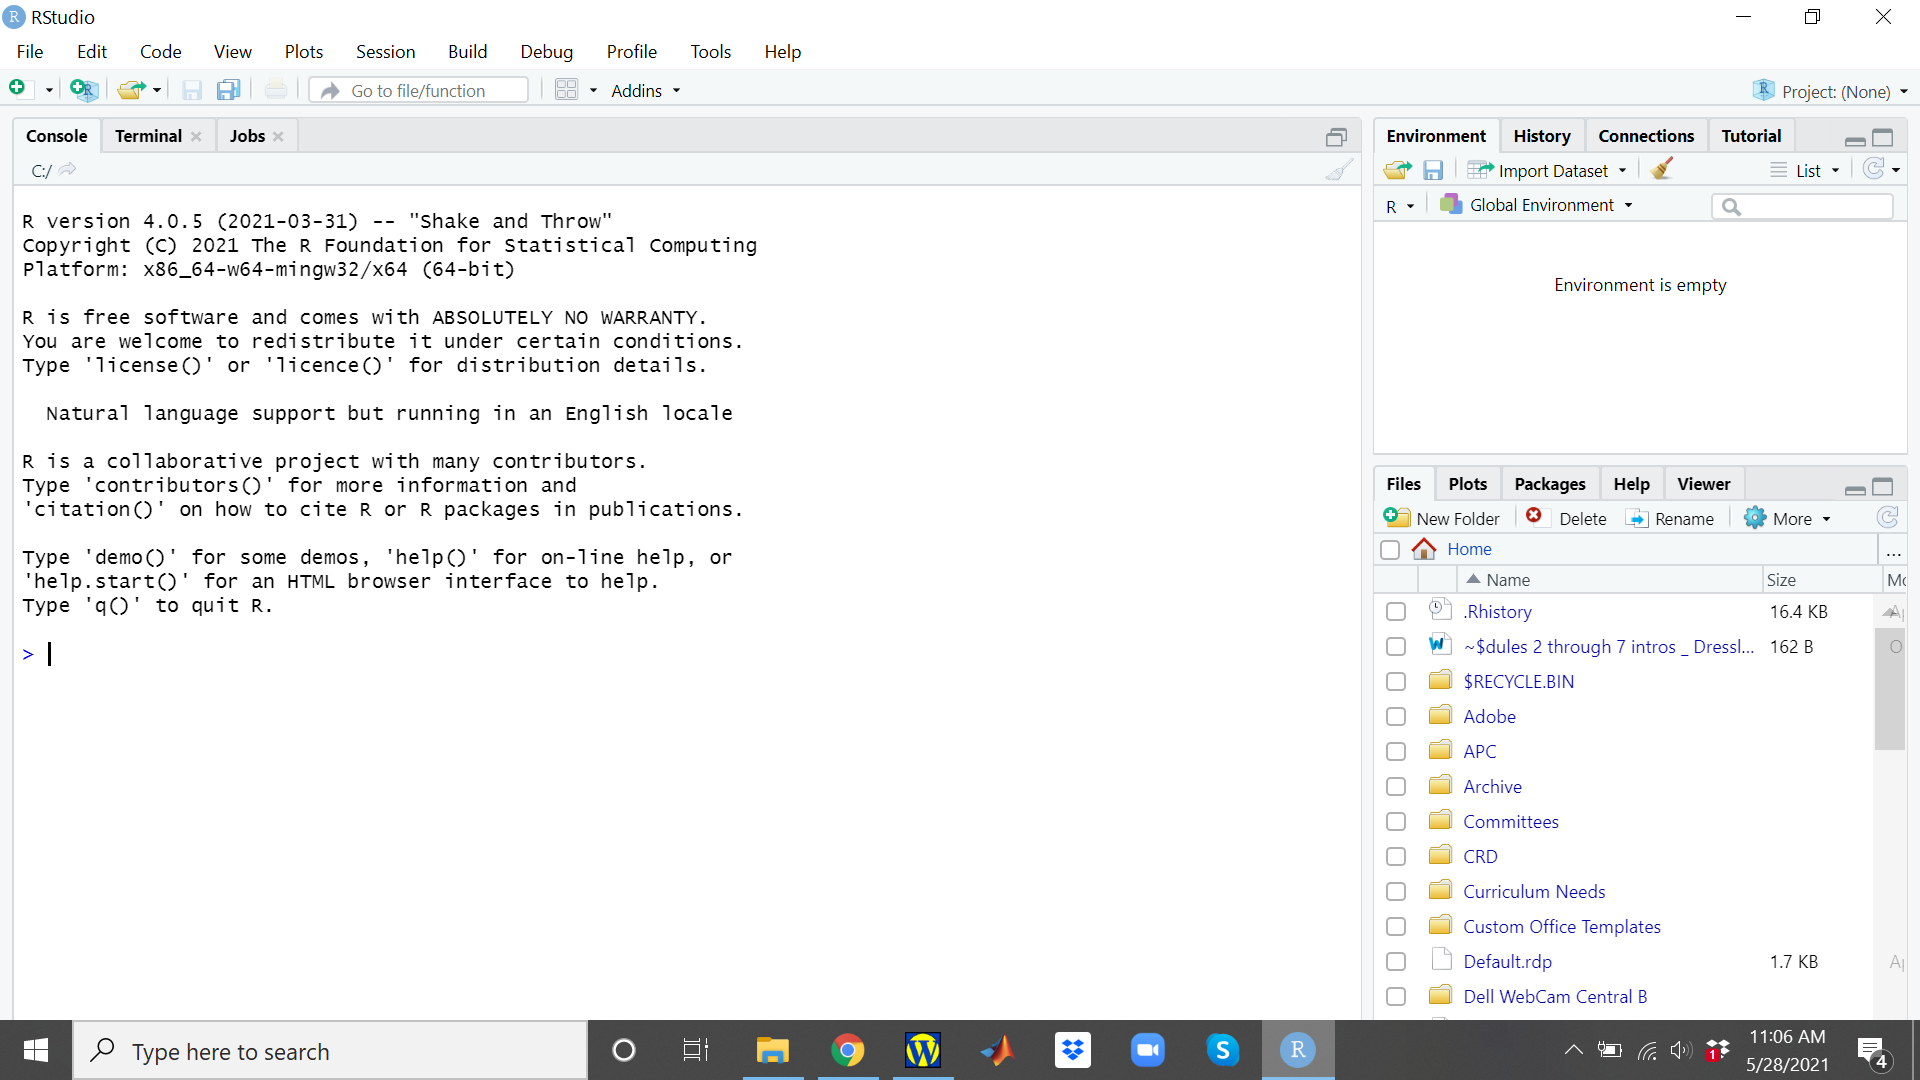
\includegraphics[width=0.75\linewidth]{images/Screenshot1} 

}

\caption{Welcome to R!}\label{fig:unnamed-chunk-29}
\end{figure}

The window on the left is your \emph{Console} which is exactly what you would see if you opened up R instead of Rstudio.\footnote{Note that we will never open R by itself, because it is easier to communicate with R through Rstudio.} The window on the upper-right is your \emph{Global Environment}. It will show you all of the data sets, variables, and result objects that are currently in R and available to you. Note that it is currently empty because we haven't done anything yet. The window on your bottom-right has several useful tabs that let us look at our folder directory (as shown) as well as any figures we generate and R packages at our disposal.

This is the default mode of Rstudio. You can input commands into the console right at the ``\textgreater{}'' and R will execute them line by line. This is fine if you wish to execute one single command, but it becomes tedious if we have a series of commands we need to execute before we arrive at our desired result. We can therefore alter this default mode by adding R-scripts.

\begin{figure}

{\centering 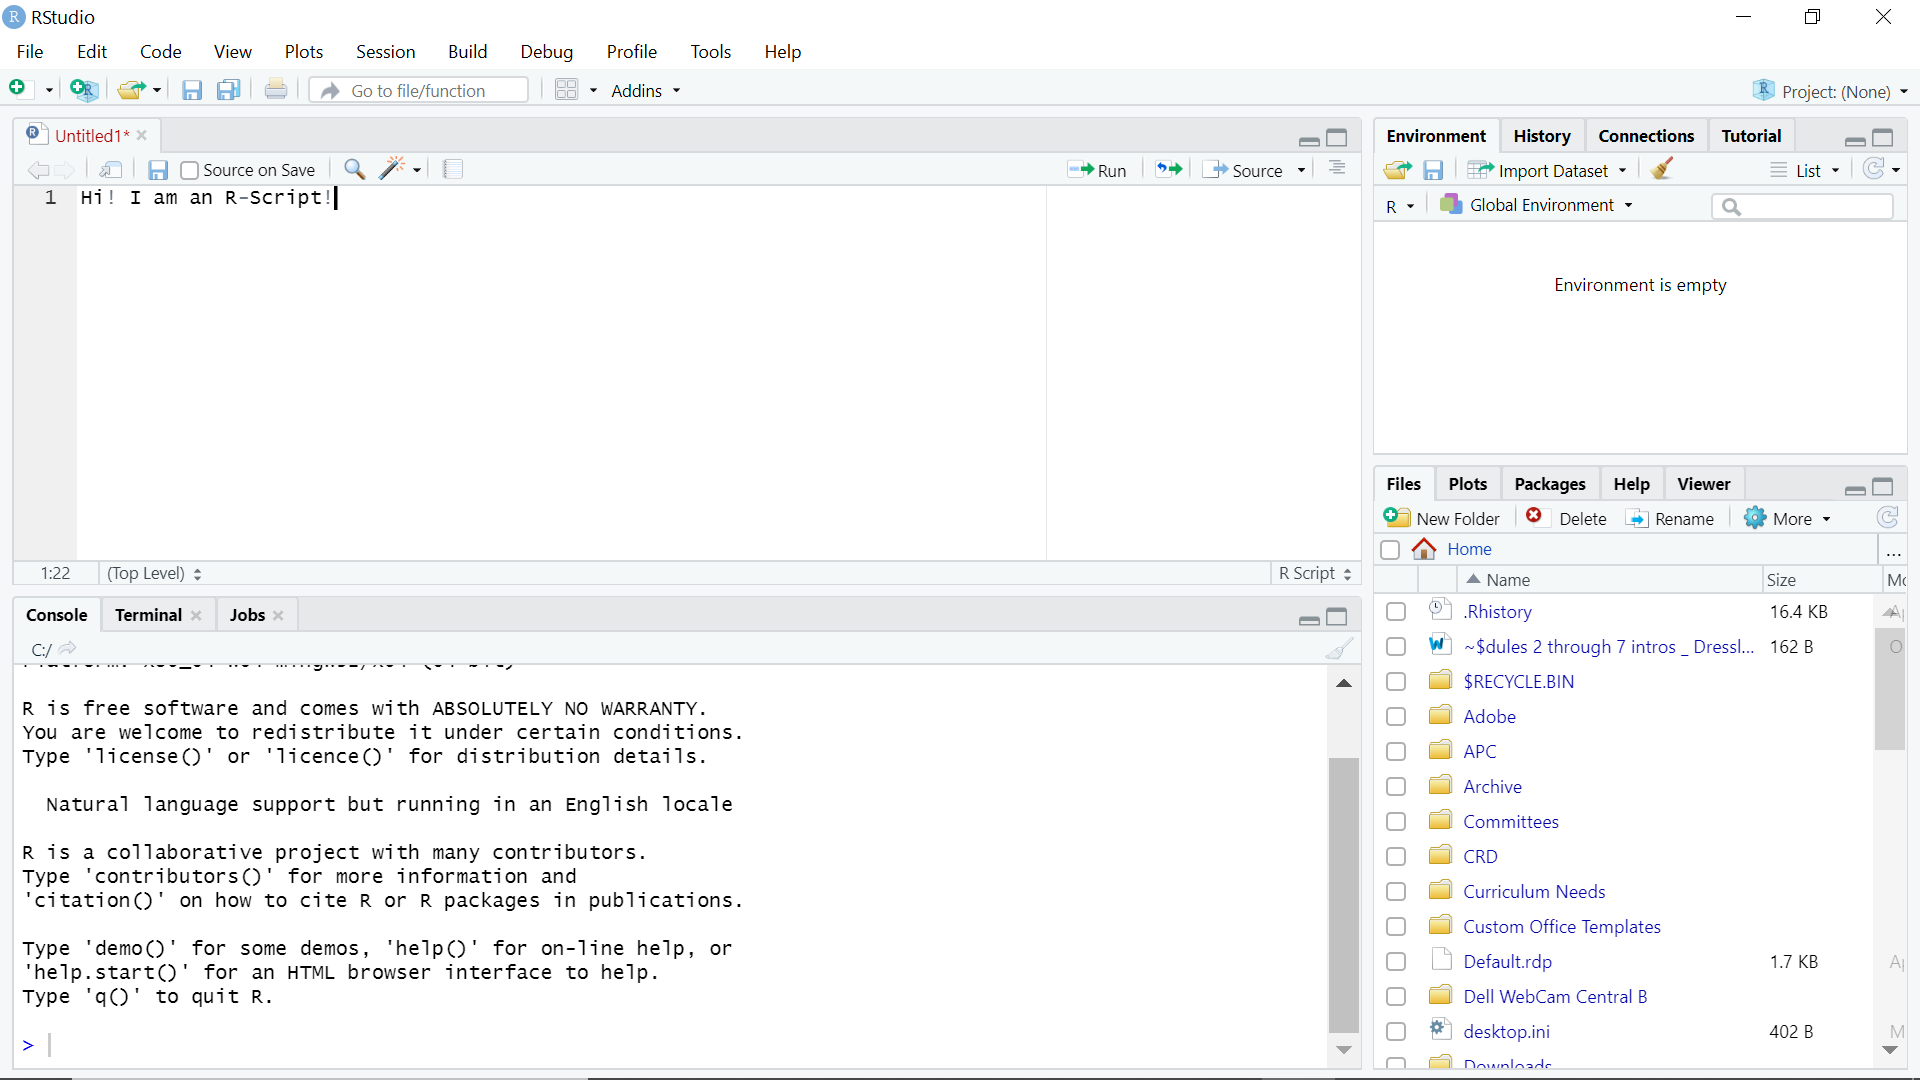
\includegraphics[width=0.75\linewidth]{images/Screenshot2} 

}

\caption{An R-script!}\label{fig:unnamed-chunk-30}
\end{figure}

Clicking on the green plus in the upper left of the screen will give you the option of opening an R-script. An R-script window will now appear and take up half of what was once our console space. An R-script is really nothing more than a text file. We can type several commands in sequence without running them line by line (which we would need to do if we typed them into the console). Once the commands are typed out, we can highlight them all and hit that run button on top. The commands get sent to the console and you're off\ldots{}

\begin{figure}

{\centering 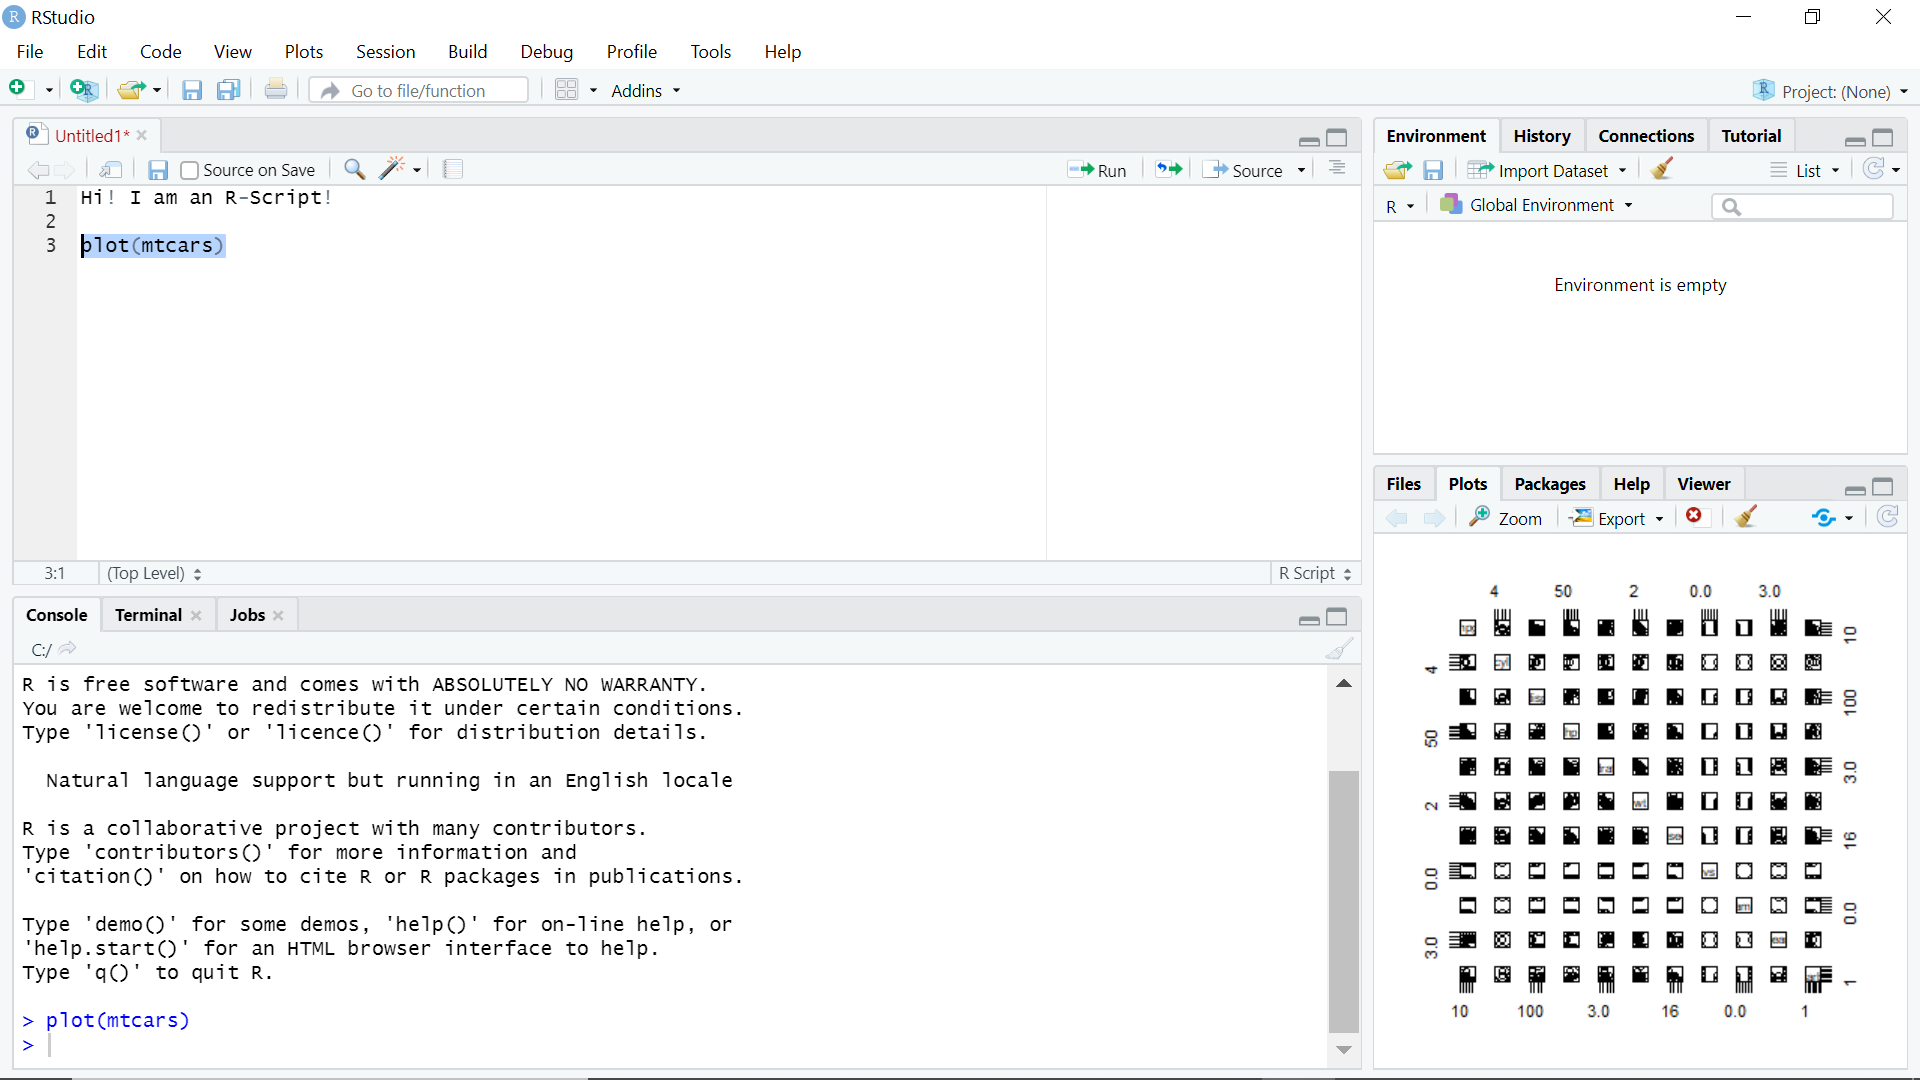
\includegraphics[width=0.75\linewidth]{images/Screenshot3} 

}

\caption{Running Commands from R-scripts!}\label{fig:unnamed-chunk-31}
\end{figure}

The picture above is just a quick example of what an R-script can do. Line 3 tells R to plot all of the variables in a dataset called \emph{mtcars}. Highlighting that line and hitting the run button sends the command to the console below, and the plot figure shows up in the Plots window. That's that!

\hypertarget{installing-packages}{%
\subsection{\texorpdfstring{Installing \emph{Packages}}{Installing Packages}}\label{installing-packages}}

R is essentially a super-powered calculator. In order for it to be able to do some of the sophisticated things we will be doing in the course, we need to install source code called \emph{packages}.

Whenever you need a package, all you need to do is type:

\begin{verbatim}
install.packages("name of package")
\end{verbatim}

Once this is done, the package is installed in your version of R and you will never need to install it again. You will need to \emph{unpack} the packages each time you want to use them by calling a \emph{library} command, but we will get to that later.

The first R-script you will run as part of your first assignment is called \emph{Install\_Packages.R}. The executable portion of the code looks like this:

\begin{verbatim}
install.packages( c("AER", "car", "dplyr", 
"fastDummies", "readxl", "xtable", "vars",
"WDI", "xts", "zoo", "wooldridge") )
\end{verbatim}

This is a simple command that asks R to download 11 packages and install them. Download and import the R-script, highlight the portion above, and hit the \emph{Run} tab at the top of the upper-left window of RStudio. A bunch of notifications will appear on the R console (lower-left window) while the list of packages will be downloaded from the mirror site you selected earlier and installed. This can take some time (about 30 mins) depending on your internet connection, so it is advised to do this when you can leave your computer alone for awhile.

\hypertarget{coding-basics}{%
\section{Coding Basics}\label{coding-basics}}

Now that your software is ready to go, this section introduces you to how R likes to be talked to. Note that the subsequent chapters are full of commands that you will need to learn when the time comes. In the meantime, here are just a few general pointers.

R is what is known as a line command computing language - meaning that it doesn't need to compile code prior to execution. That being said, try the following command at the prompt in your console (\textgreater):

\begin{Shaded}
\begin{Highlighting}[]
\DecValTok{12} \SpecialCharTok{+} \DecValTok{4}
\end{Highlighting}
\end{Shaded}

\begin{verbatim}
## [1] 16
\end{verbatim}

See? Just a big calculator.

\hypertarget{assigning-objects}{%
\subsection{Assigning Objects}\label{assigning-objects}}

We declare variable names and other data objects by \emph{assigning} things names. For example, we can repeat the calculation above by first assigning some variables the same numbers:

\begin{Shaded}
\begin{Highlighting}[]
\NormalTok{BIG }\OtherTok{\textless{}{-}} \DecValTok{12}
\NormalTok{SMALL }\OtherTok{\textless{}{-}} \DecValTok{4}
\NormalTok{(TOTAL }\OtherTok{\textless{}{-}}\NormalTok{ BIG }\SpecialCharTok{+}\NormalTok{ SMALL)}
\end{Highlighting}
\end{Shaded}

\begin{verbatim}
## [1] 16
\end{verbatim}

Notice that all of these variable names should now be in your global environment (upper-right window). The reason why 16 was returned on the console is because we put the last command in parentheses. That is the \emph{print to screen} command.

You might be asking why R simply doesn't use an equal sign in stead of the assign sign. The answer is that we will be assigning names to output objects that contain much more than a single number. Things like regression output is technically \emph{assigned} a name, so we are simple being consistent.

\hypertarget{listing-adding-and-removing}{%
\subsection{Listing, Adding, and Removing}\label{listing-adding-and-removing}}

We can list all objects in our global environment using the list command: ls()

\begin{Shaded}
\begin{Highlighting}[]
\FunctionTok{ls}\NormalTok{()}
\end{Highlighting}
\end{Shaded}

\begin{verbatim}
##   [1] "AL"          "alpha"       "AUTO"        "B1"          "Bhat0"       "Bhat1"       "BIG"        
##   [8] "car"         "CARDATA"     "CARDATA2"    "CARGSP"      "CDdata"      "CGDP"        "CM"         
##  [15] "CREG"        "D"           "DENGSP"      "df"          "DGDP"        "DS"          "DTRND"      
##  [22] "e"           "eps"         "EPS"         "Fcrit"       "fit"         "fitpoints"   "Fstat"      
##  [29] "grid.lines"  "h"           "hprice1"     "i"           "i1"          "i2"          "j"          
##  [36] "k"           "left"        "LEFT"        "LFT"         "Lifetime"    "Lifetime1"   "Lifetime2"  
##  [43] "m"           "M"           "MDAT"        "Mode"        "mtcars"      "mu"          "MULTI2"     
##  [50] "n"           "N"           "P"           "PARK"        "probability" "Pval"        "R"          
##  [57] "R2r"         "R2u"         "Rate"        "REG"         "REG1"        "REG2"        "REG3"       
##  [64] "REG4"        "RES"         "Revenue"     "RHT"         "right"       "RIGHT"       "RREG"       
##  [71] "S"           "SBhat1"      "Sig"         "sigma"       "SMALL"       "t"           "t_values"   
##  [78] "tcrit"       "TOTAL"       "tstat"       "UREG"        "wage1"       "x"           "X"          
##  [85] "x.pred"      "X1"          "X2"          "X3"          "Xbar"        "Xcrap"       "xfit"       
##  [92] "xtick"       "xy"          "Y"           "y.pred"      "Y1"          "Y2"          "Y3"         
##  [99] "yfit"        "Yhat"        "Yz"          "Z"           "z.pred"      "Zcrit"       "Zstat"
\end{verbatim}

As we already showed, we can add new variables by simply assigning names to our calculations.

\begin{Shaded}
\begin{Highlighting}[]
\NormalTok{TOTAL.SQUARED }\OtherTok{\textless{}{-}}\NormalTok{ TOTAL}\SpecialCharTok{\^{}}\DecValTok{2}
\end{Highlighting}
\end{Shaded}

If you ever wanted to remove some variables from your global environment, you can use the remove command: rm(\emph{name of variable})

\begin{Shaded}
\begin{Highlighting}[]
\FunctionTok{rm}\NormalTok{(TOTAL.SQUARED)}
\end{Highlighting}
\end{Shaded}

\hypertarget{loading-data}{%
\subsection{Loading Data}\label{loading-data}}

R can handle data in almost any format imaginable. The main data format we will consider in this class is a trusty old MS Excel file. There are two ways to load data\ldots{}

\textbf{1. The Direct Way}

Once you locate a data file on your computer, you can direct R to import the file and assign it any name you want. The example below imports a dataset of automobile sales called AUTO\_SA.xlsx and names it \emph{CARDATA}.

\begin{Shaded}
\begin{Highlighting}[]
\FunctionTok{library}\NormalTok{(readxl)}
\NormalTok{CARDATA }\OtherTok{\textless{}{-}} \FunctionTok{read\_excel}\NormalTok{(}\StringTok{"data/AUTO\_SA.xlsx"}\NormalTok{)}
\end{Highlighting}
\end{Shaded}

The term \emph{``data/AUTO\_SA.xlsx''} is the exact location on my computer for this data file. It is recommended that you put all of you data files somewhere easy to access. Like a single folder directly on your C drive.

\textbf{2. The Indirect (but easy) Way}

You can also import data directly into R through Rstudio.

\begin{enumerate}
\def\labelenumi{\arabic{enumi}.}
\item
  Use the files tab (bottom-right window) and locate the data file you want to import.
\item
  Left-click on file and select \emph{Import Dataset\ldots{}}
\item
  The import window opens and previews your data.
\item
  If everything looks good, hit \emph{Import} and your done.
\end{enumerate}

Note that the import window in step 3 has a \emph{code preview} section which is actually writing the code needed to import the dataset. It will look exactly like what your code would need to look like in order to import data the direct way. You can refer to that for future reference.

\hypertarget{manipulating-data}{%
\subsection{Manipulating Data}\label{manipulating-data}}

You should now have a dataset named \emph{CARDATA} imported into your global environment. You can examine the names of the variables inside the dataset using the list command - only this time we reference the name of the dataset.

\begin{Shaded}
\begin{Highlighting}[]
\FunctionTok{ls}\NormalTok{(CARDATA)}
\end{Highlighting}
\end{Shaded}

\begin{verbatim}
## [1] "AUTOSALE" "CPI"      "DATE"     "INDEX"    "MONTH"    "YEAR"
\end{verbatim}

When referencing a variable within a dataset, you must reference both the names of the dataset and variable so R knows where to get it. The syntax is:

Dataset\$Variable

For example, if we reference the variable \emph{AUTOSALE} by stating that it is in the CARDATA dataset.

CARDATA\$AUTOSALE

We can now manipulate and store variables within the dataset by creating variables for what ever we need. For example, we can create a variable for real autosales by dividing autosales by the consumer price index (CPI).

\begin{Shaded}
\begin{Highlighting}[]
\NormalTok{CARDATA}\SpecialCharTok{$}\NormalTok{RSALES }\OtherTok{\textless{}{-}}\NormalTok{ CARDATA}\SpecialCharTok{$}\NormalTok{AUTOSALE }\SpecialCharTok{/}\NormalTok{ CARDATA}\SpecialCharTok{$}\NormalTok{CPI}
\FunctionTok{ls}\NormalTok{(CARDATA)}
\end{Highlighting}
\end{Shaded}

\begin{verbatim}
## [1] "AUTOSALE" "CPI"      "DATE"     "INDEX"    "MONTH"    "RSALES"   "YEAR"
\end{verbatim}

\hypertarget{subsetting-data}{%
\subsection{Subsetting Data}\label{subsetting-data}}

Sometimes our dataset will contain more information than we need. Let us narrow down our dataset to see how we can get rid of unwanted data. You should see a little Excel looking icon to the left of the name CARDATA up in the global environment window. If you click on it, you should see the following:

\begin{figure}

{\centering 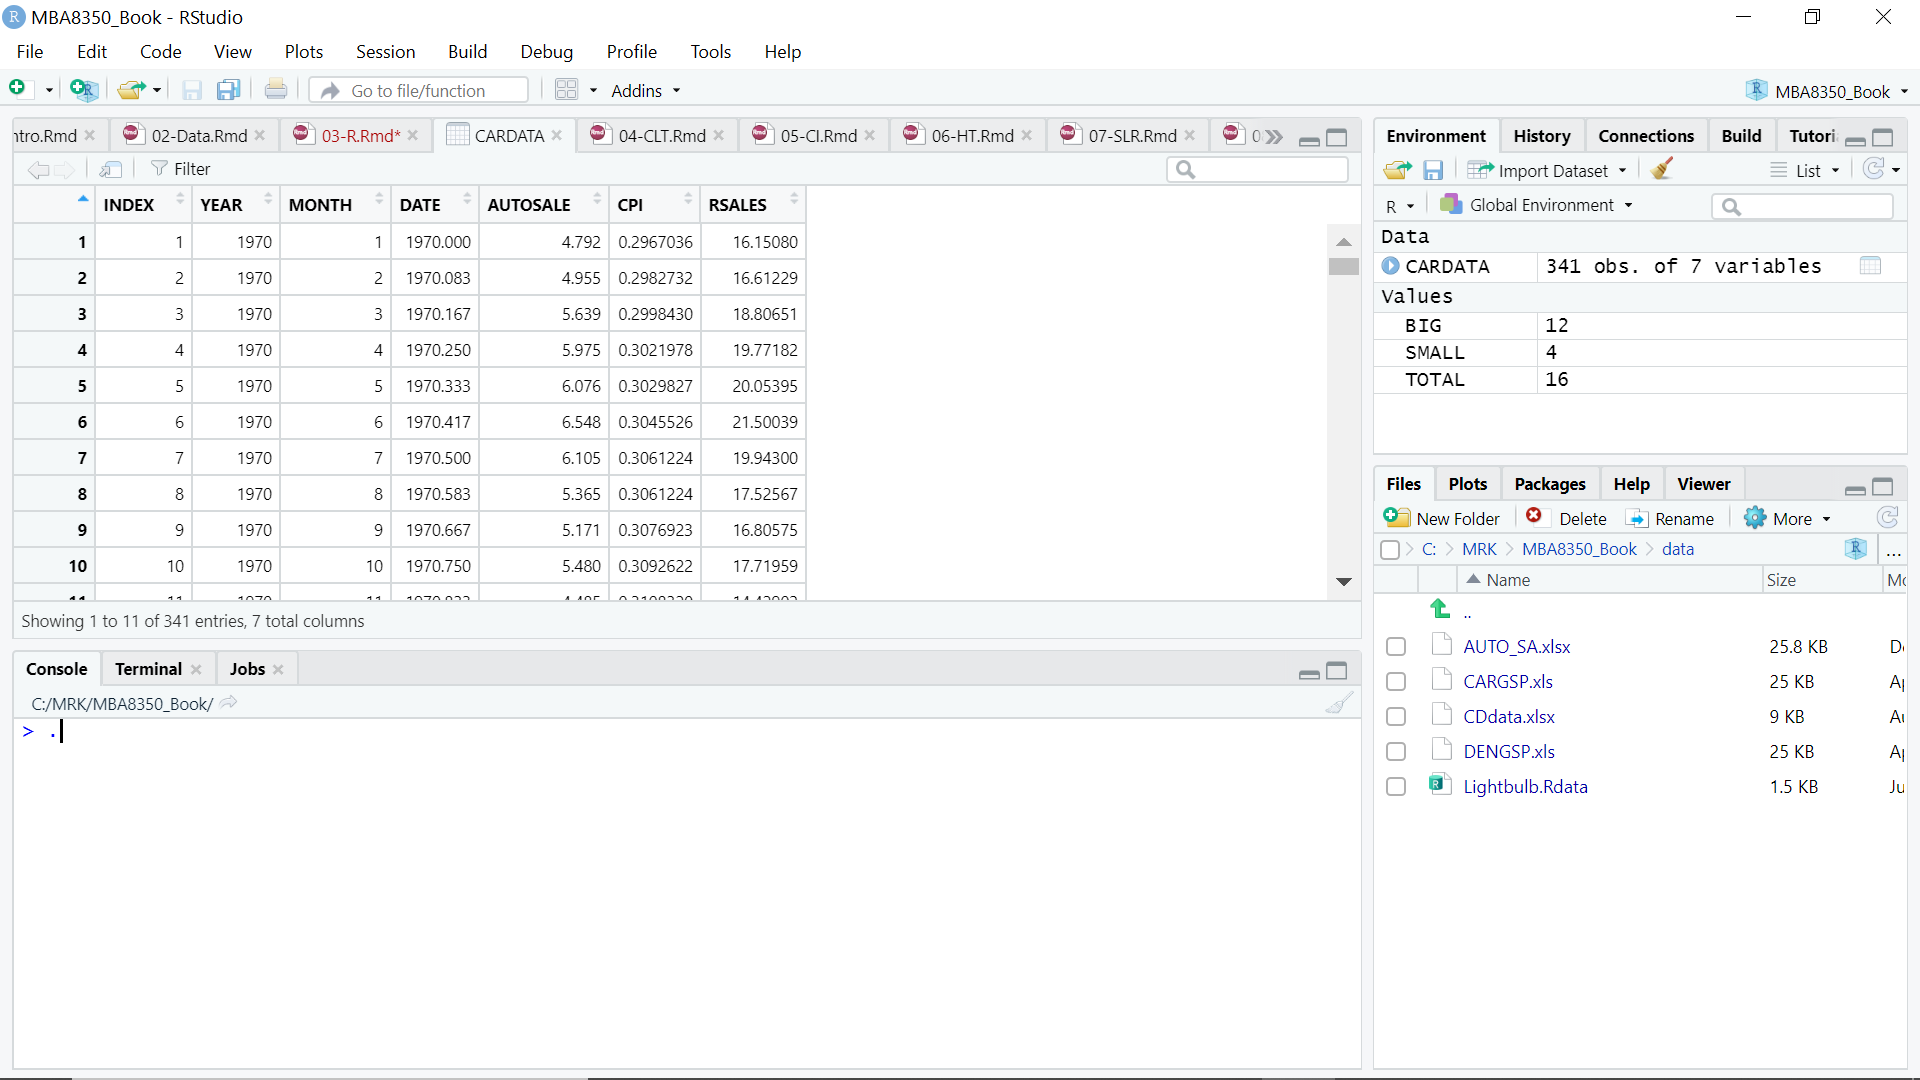
\includegraphics[width=0.75\linewidth]{images/Screenshot4} 

}

\caption{A Dataset in R}\label{fig:unnamed-chunk-40}
\end{figure}

Thinking of the data set as a matrix with 341 rows and 7 columns will help us understand the code needed to select specific portions of this data.

Note that the variable MONTH cycles from 1 to 12 indicating the months of the year. Suppose we only want to analyze the 12th month of each year (i.e., December). We can do this by creating a new dataset that keeps only the rows associated with the 12 month.

\begin{Shaded}
\begin{Highlighting}[]
\NormalTok{CARDATA2 }\OtherTok{\textless{}{-}}\NormalTok{ CARDATA[CARDATA}\SpecialCharTok{$}\NormalTok{MONTH}\SpecialCharTok{==}\DecValTok{12}\NormalTok{,]}
\end{Highlighting}
\end{Shaded}

What the above code does is treat the dataset CARDATA as a matrix and lists it as {[}rows,columns{]}. The rows instruction is to only keep rows where the month is 12. The columns instruction is left blank, because we want to keep all columns.

\hypertarget{data-visualization}{%
\section{Data Visualization}\label{data-visualization}}

R is absolutely brilliant when it comes to data visualization, and this section will only scratch the surface. We will go over some basic data visualizations using the built-in features of R. There are a lot of resources out there that covers a separate R package called ggplot. It's a handy package, but knowing the features discussed here will be sufficient for our course as well as give you some background that will help you push ggplot farther (if need be).

\hypertarget{histograms}{%
\subsection{Histograms}\label{histograms}}

A histogram breaks data observations into bins (or breaks) and shows the frequency distribution of these bins. We will use this to consider probability distributions, but it also helps us get an idea of the distributional properties of any data sample.

Let us continue to analyze the car dataset we created above:

\begin{Shaded}
\begin{Highlighting}[]
\FunctionTok{hist}\NormalTok{(CARDATA}\SpecialCharTok{$}\NormalTok{RSALES)}
\end{Highlighting}
\end{Shaded}

\begin{center}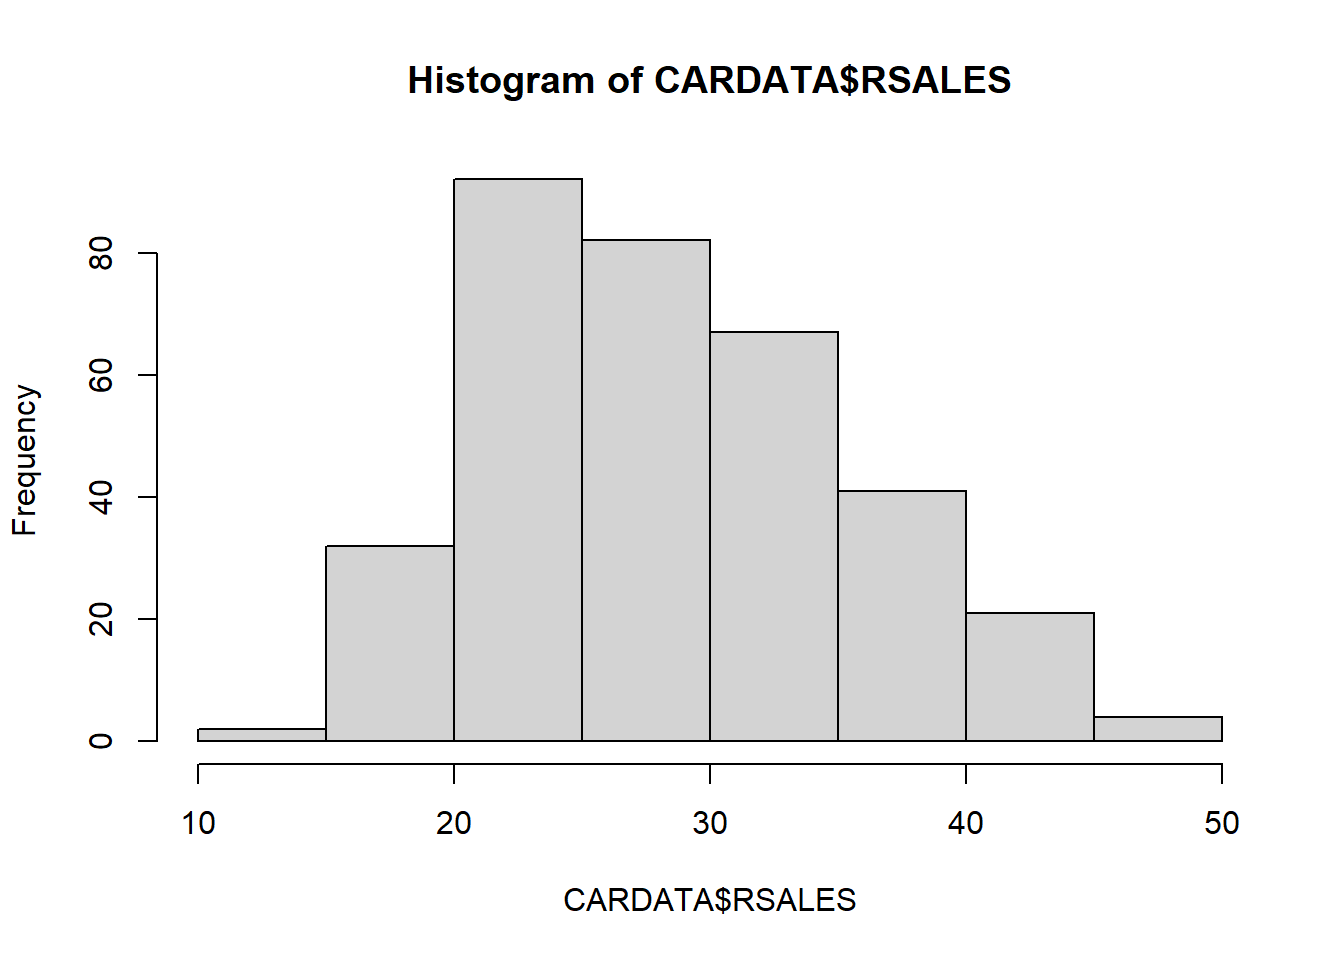
\includegraphics{MBA8350book_files/figure-latex/unnamed-chunk-42-1} \end{center}

We can fancy this up by changing the title (main), labels (xlab), number of bins (breaks), and color (col). We will do this one at a time by creating a 2 by 2 set of figures using the par(mfrow=c(2,2)) command. This command \emph{partitions} the plot window into a 2x2 series of subplots.

\begin{Shaded}
\begin{Highlighting}[]
\FunctionTok{par}\NormalTok{(}\AttributeTok{mfrow=}\FunctionTok{c}\NormalTok{(}\DecValTok{2}\NormalTok{,}\DecValTok{2}\NormalTok{))}
\FunctionTok{hist}\NormalTok{(CARDATA}\SpecialCharTok{$}\NormalTok{RSALES,}\AttributeTok{main =} \StringTok{"Real Auto Sales"}\NormalTok{)}
\FunctionTok{hist}\NormalTok{(CARDATA}\SpecialCharTok{$}\NormalTok{RSALES,}\AttributeTok{main =} \StringTok{"Real Auto Sales"}\NormalTok{,}
     \AttributeTok{xlab =} \StringTok{"Real Sales"}\NormalTok{)}
\FunctionTok{hist}\NormalTok{(CARDATA}\SpecialCharTok{$}\NormalTok{RSALES,}\AttributeTok{main =} \StringTok{"Real Auto Sales"}\NormalTok{,}
     \AttributeTok{xlab =} \StringTok{"Real Sales"}\NormalTok{,}
     \AttributeTok{breaks =} \DecValTok{40}\NormalTok{)}
\FunctionTok{hist}\NormalTok{(CARDATA}\SpecialCharTok{$}\NormalTok{RSALES,}\AttributeTok{main =} \StringTok{"Real Auto Sales"}\NormalTok{,}
     \AttributeTok{xlab =} \StringTok{"Real Sales"}\NormalTok{,}
     \AttributeTok{breaks =} \DecValTok{40}\NormalTok{,}
     \AttributeTok{col =} \StringTok{"pink"}\NormalTok{)}
\end{Highlighting}
\end{Shaded}

\begin{center}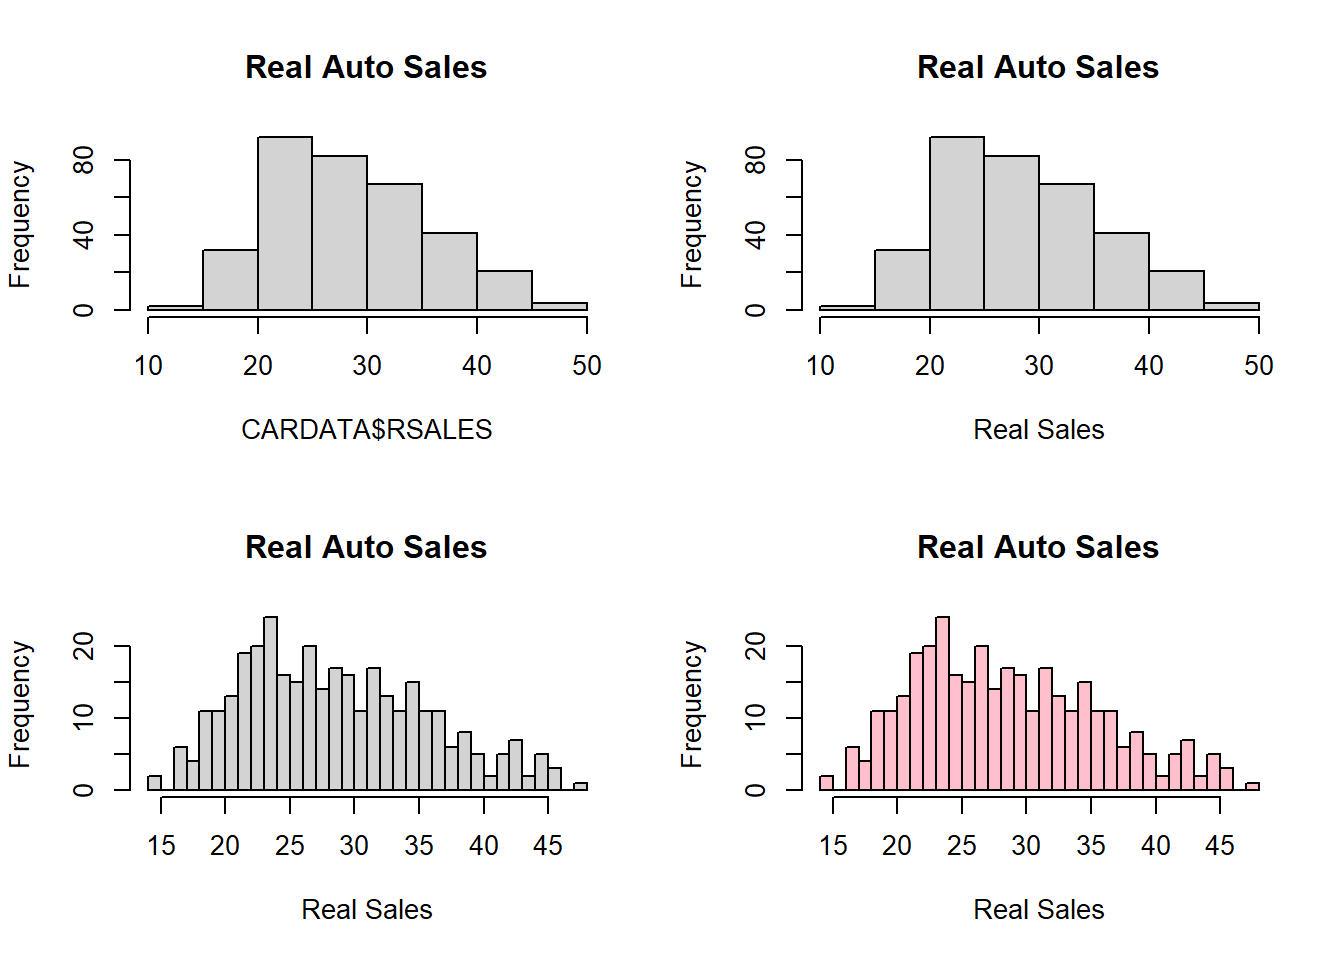
\includegraphics{MBA8350book_files/figure-latex/unnamed-chunk-43-1} \end{center}

\hypertarget{line-bar-and-scatter-plots}{%
\subsection{Line, bar, and Scatter Plots}\label{line-bar-and-scatter-plots}}

The plot command can visualize the relationship between two variables or just one variable in order. The barplot command is similar to a single-variable plot.

We can look at the nominal sales data in a line plot by specifying the type of plot as ``l''. A barplot delivers the same information, but just looks different.

\begin{Shaded}
\begin{Highlighting}[]
\FunctionTok{par}\NormalTok{(}\AttributeTok{mfrow=}\FunctionTok{c}\NormalTok{(}\DecValTok{2}\NormalTok{,}\DecValTok{1}\NormalTok{))}
\FunctionTok{plot}\NormalTok{(CARDATA}\SpecialCharTok{$}\NormalTok{AUTOSALE, }\AttributeTok{type =} \StringTok{"l"}\NormalTok{)}
\FunctionTok{barplot}\NormalTok{(CARDATA}\SpecialCharTok{$}\NormalTok{AUTOSALE)}
\end{Highlighting}
\end{Shaded}

\begin{center}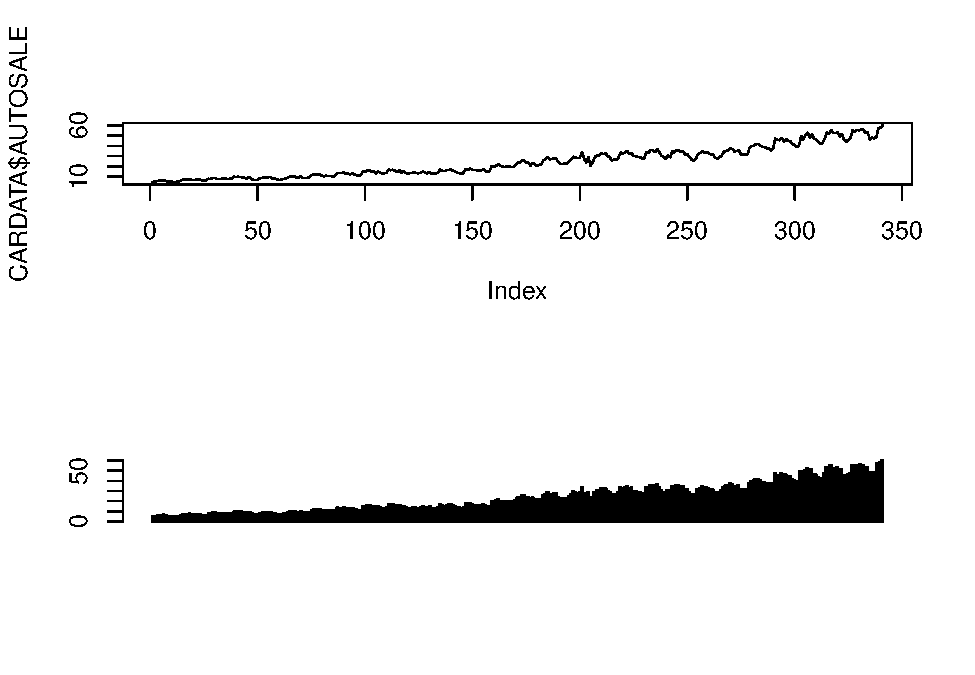
\includegraphics{MBA8350book_files/figure-latex/unnamed-chunk-44-1} \end{center}

We can look at relationships using the default values of the plot command.

\begin{Shaded}
\begin{Highlighting}[]
\FunctionTok{plot}\NormalTok{(CARDATA}\SpecialCharTok{$}\NormalTok{CPI,CARDATA}\SpecialCharTok{$}\NormalTok{AUTOSALE)}
\end{Highlighting}
\end{Shaded}

\begin{center}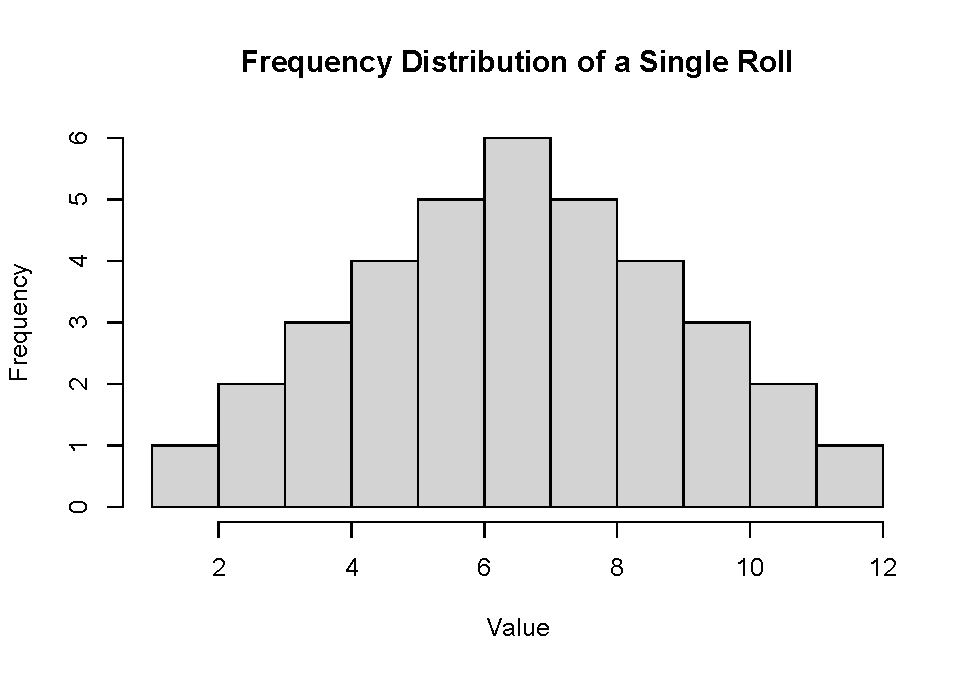
\includegraphics{MBA8350book_files/figure-latex/unnamed-chunk-45-1} \end{center}

You will see plenty of these plots throughout these notes, and they will get increasingly more sophisticated with titles, colors, etc.

\hypertarget{boxplots}{%
\subsection{Boxplots}\label{boxplots}}

Box Plot illustrate the minimum, the 25th, 50th (median), 75th percentiles and the maximum. It is useful for visualizing the spread of the data.

\begin{Shaded}
\begin{Highlighting}[]
\FunctionTok{boxplot}\NormalTok{(CARDATA}\SpecialCharTok{$}\NormalTok{AUTOSALE)}
\end{Highlighting}
\end{Shaded}

\begin{center}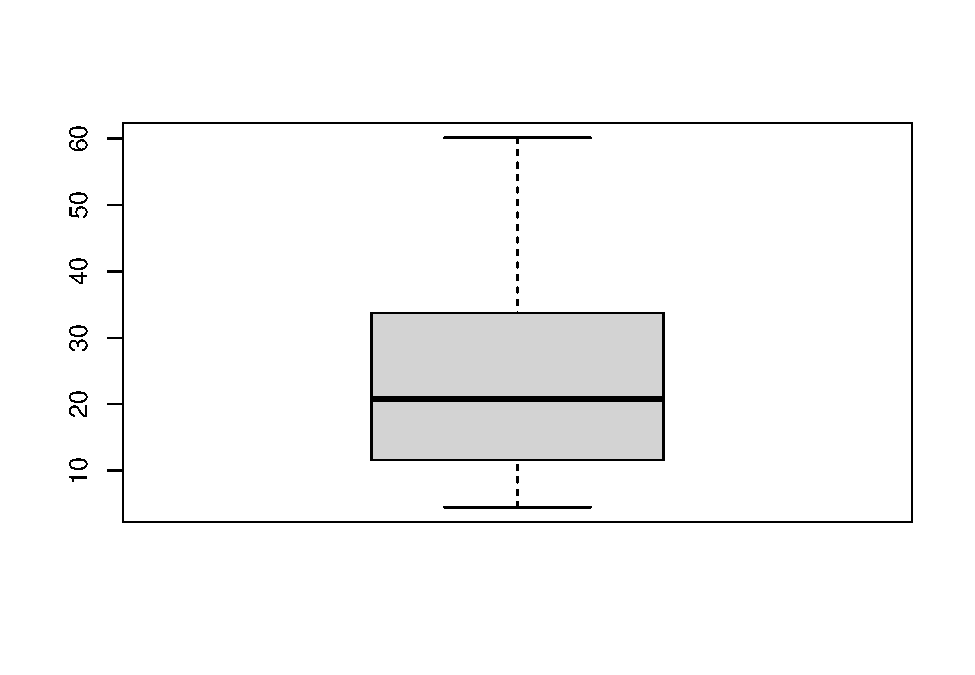
\includegraphics{MBA8350book_files/figure-latex/unnamed-chunk-46-1} \end{center}

We can also examine these five numbers within groups according to some other variable. Lets look at this breakdown of auto sales per month of the year.

\begin{Shaded}
\begin{Highlighting}[]
\FunctionTok{boxplot}\NormalTok{(CARDATA}\SpecialCharTok{$}\NormalTok{AUTOSALE}\SpecialCharTok{\textasciitilde{}}\NormalTok{CARDATA}\SpecialCharTok{$}\NormalTok{MONTH)}
\end{Highlighting}
\end{Shaded}

\begin{center}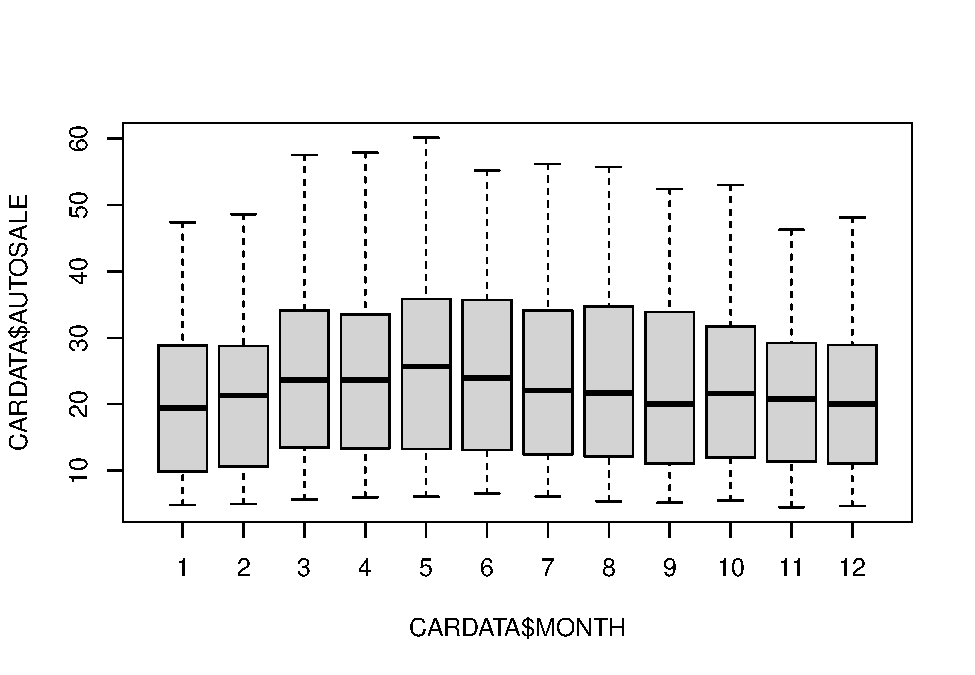
\includegraphics{MBA8350book_files/figure-latex/unnamed-chunk-47-1} \end{center}

\hypertarget{much-more-out-there}{%
\subsection{Much more out there}\label{much-more-out-there}}

While this basically covers most of the plots we will need for the course, there is a ton more out there. The interested reader can consult a \emph{free} book on the matter.

\url{https://rkabacoff.github.io/datavis/}

However deep you want to go, I hope you have seen that data visualization in R is a heck of a lot easier than in Excel.\footnote{For example, a histogram in MS Excel takes about 20 minutes for me to create for each one!}

\hypertarget{CLT}{%
\chapter{The Central Limit Theorem}\label{CLT}}

The \textbf{Central Limit Theorem} (henceforth, CLT) is one of the most important conceptual parts of inferential statistics. It is the essential reason why we can make educated guesses regarding the parameters of a population using information on the statistics of a sample. The CLT will going on in the background of every subsequent chapter of this course companion. Doing statistics without fully understanding the CLT is simply going through the motions. You will not be able to fully appreciate inferential statistics without knowing what is really going on beneath the hood.

\hypertarget{the-clt-formally}{%
\section{The CLT (Formally)}\label{the-clt-formally}}

Recall the concept of sampling distribution from chapter 2. For every randomly selected sample (i.e., a subset of the population), you can calculate a sample mean. If you were to repeatedly collect random samples and record their sample means, then you would be able to construct a \emph{sampling distribution} of the sample mean values. Looking at the frequency of values (i.e., a frequency distribution) would give you an idea of where you think the mean value from the next sample you would randomly draw will be. The statistical properties of this sampling distribution is where the educated guessing is coming from.

So here is the CLT formally\ldots{}

\begin{quote}
The central limit theorem states that if you have a population with mean \(\mu\) and standard deviation \(\sigma\) and take sufficiently large random samples of size \(n\) from the population with replacement, then the distribution of the sample means will be approximately normally distributed.
\end{quote}

There are some finer details to note.

\begin{itemize}
\item
  Given the population parameters \(\mu\) and \(\sigma\), the resulting sampling distribution will be a normal distribution with mean \(\mu\) and standard deviation \(\sigma / \sqrt{n}\).
\item
  This will hold true regardless of whether or not the source population is normal, provided the sample size is sufficiently large (usually \(n > 30\)).
\item
  If the population distribution is normal, then the theorem holds true even for samples smaller than 30.
\item
  This means that we can use the normal probability distribution to quantify uncertainty when making inferences about a population mean based on the sample mean.
\end{itemize}

Now, the CLT can be proven - but I think it's better to illustrate the CLT with a couple of examples.

\hypertarget{application-1-a-sampling-distribution-with-a-known-population}{%
\section{Application 1: A Sampling Distribution with a Known Population}\label{application-1-a-sampling-distribution-with-a-known-population}}

The first application presents sampling distributions for a random process where we know the underlying process of the population: The rolling of two die.

Suppose you worked for a gaming commission and placed in charge of making sure the dice at a casino were fair. \textbf{We know} that the (population) average roll of 2 fair die is 7 while the standard deviation is 2.45.\footnote{The mean of a single dice throw is 3.5,
  \[ 3.5 = (1 + 2 + 3 + 4 + 5 + 6) / 6\]
  and the expected value of two independent dice is the sum of expected values of each die. Standard deviation can be calculated using this mean value and the formula presented earlier.}

It wouldn't be fair for you to test a set of dice by rolling them once because there is a large probability of rolling a number other than 7. In particular, there are 36 possible outcomes of rolling two die and only 6 of those outcomes equal 7. This means that although 7 is the highest probability single outcome, there is a much higher probability of rolling a number other than 7 (\emph{ever play craps?}).

\begin{center}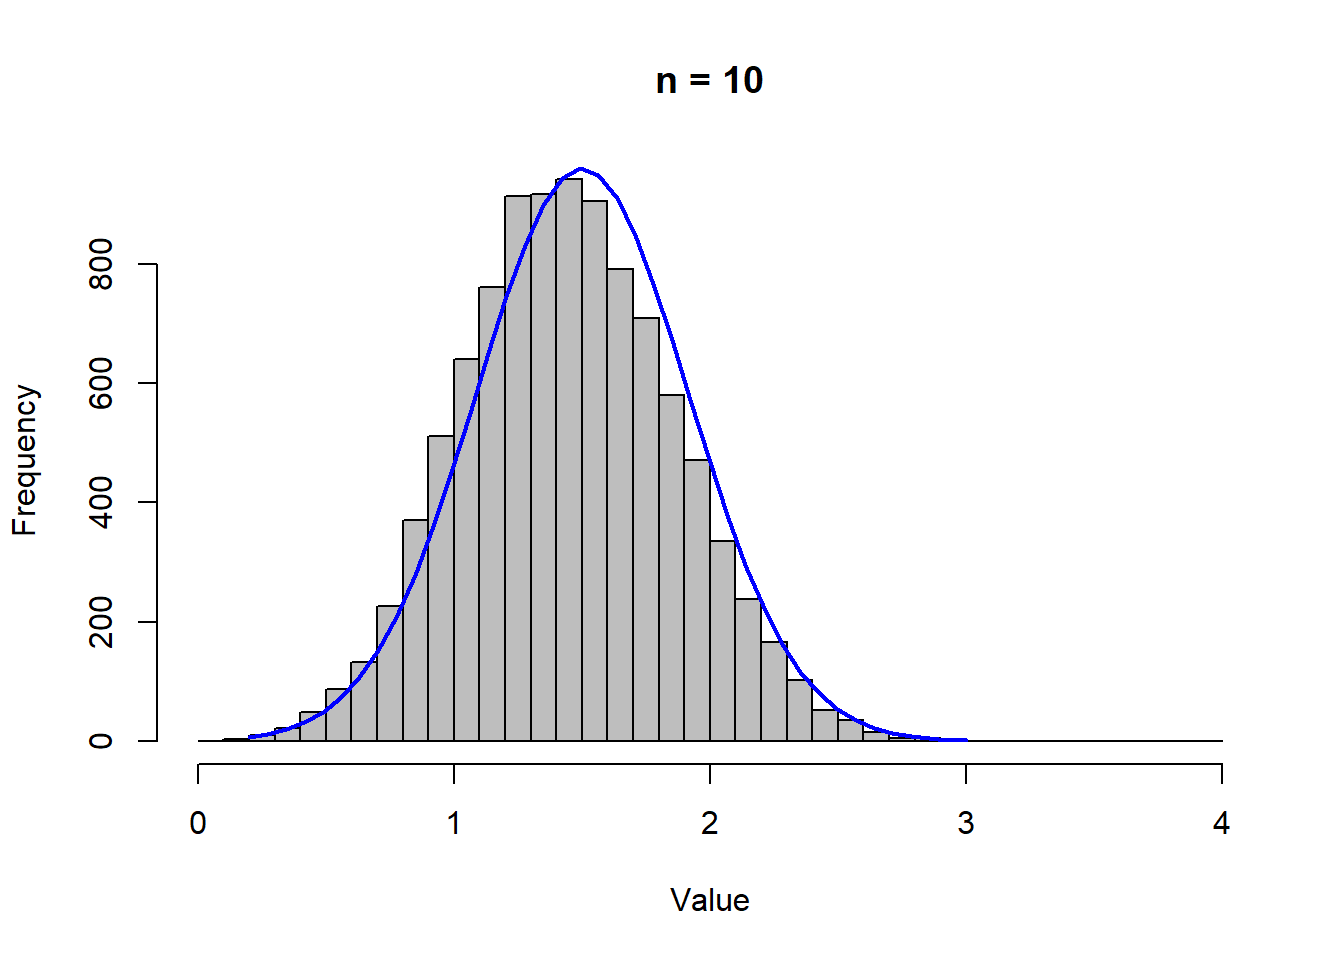
\includegraphics{MBA8350book_files/figure-latex/unnamed-chunk-49-1} \end{center}

The figure above is the population distribution of rolling two die. The average (mean) value is 7, the range of possible outcomes are between 2 and 12, and the standard deviation is a number that represents the dispersion of individual values around the mean. If you were to roll two die, then the outcome of that roll is conceptually a draw from this distribution.

Since we don't want to wrongfully accuse the casino of cheating, we need to roll the dice a few times to get an idea of what the average roll value is. If it is fair dice, then we know they will roll a 7 on average - but that means we would need to roll the dice an \emph{infinite} amount of times to achieve this. To be realistic, lets settle on a number of rolls to be generally given by \(n\). If we choose \(n=5\), then that means we roll the dice 5 times, record the roll each time, and then record the average. This is a sample average of a sample of size 5. We could do this for \(n=10\), \(n=30\), \(n=300\), etc.

\begin{figure}

{\centering 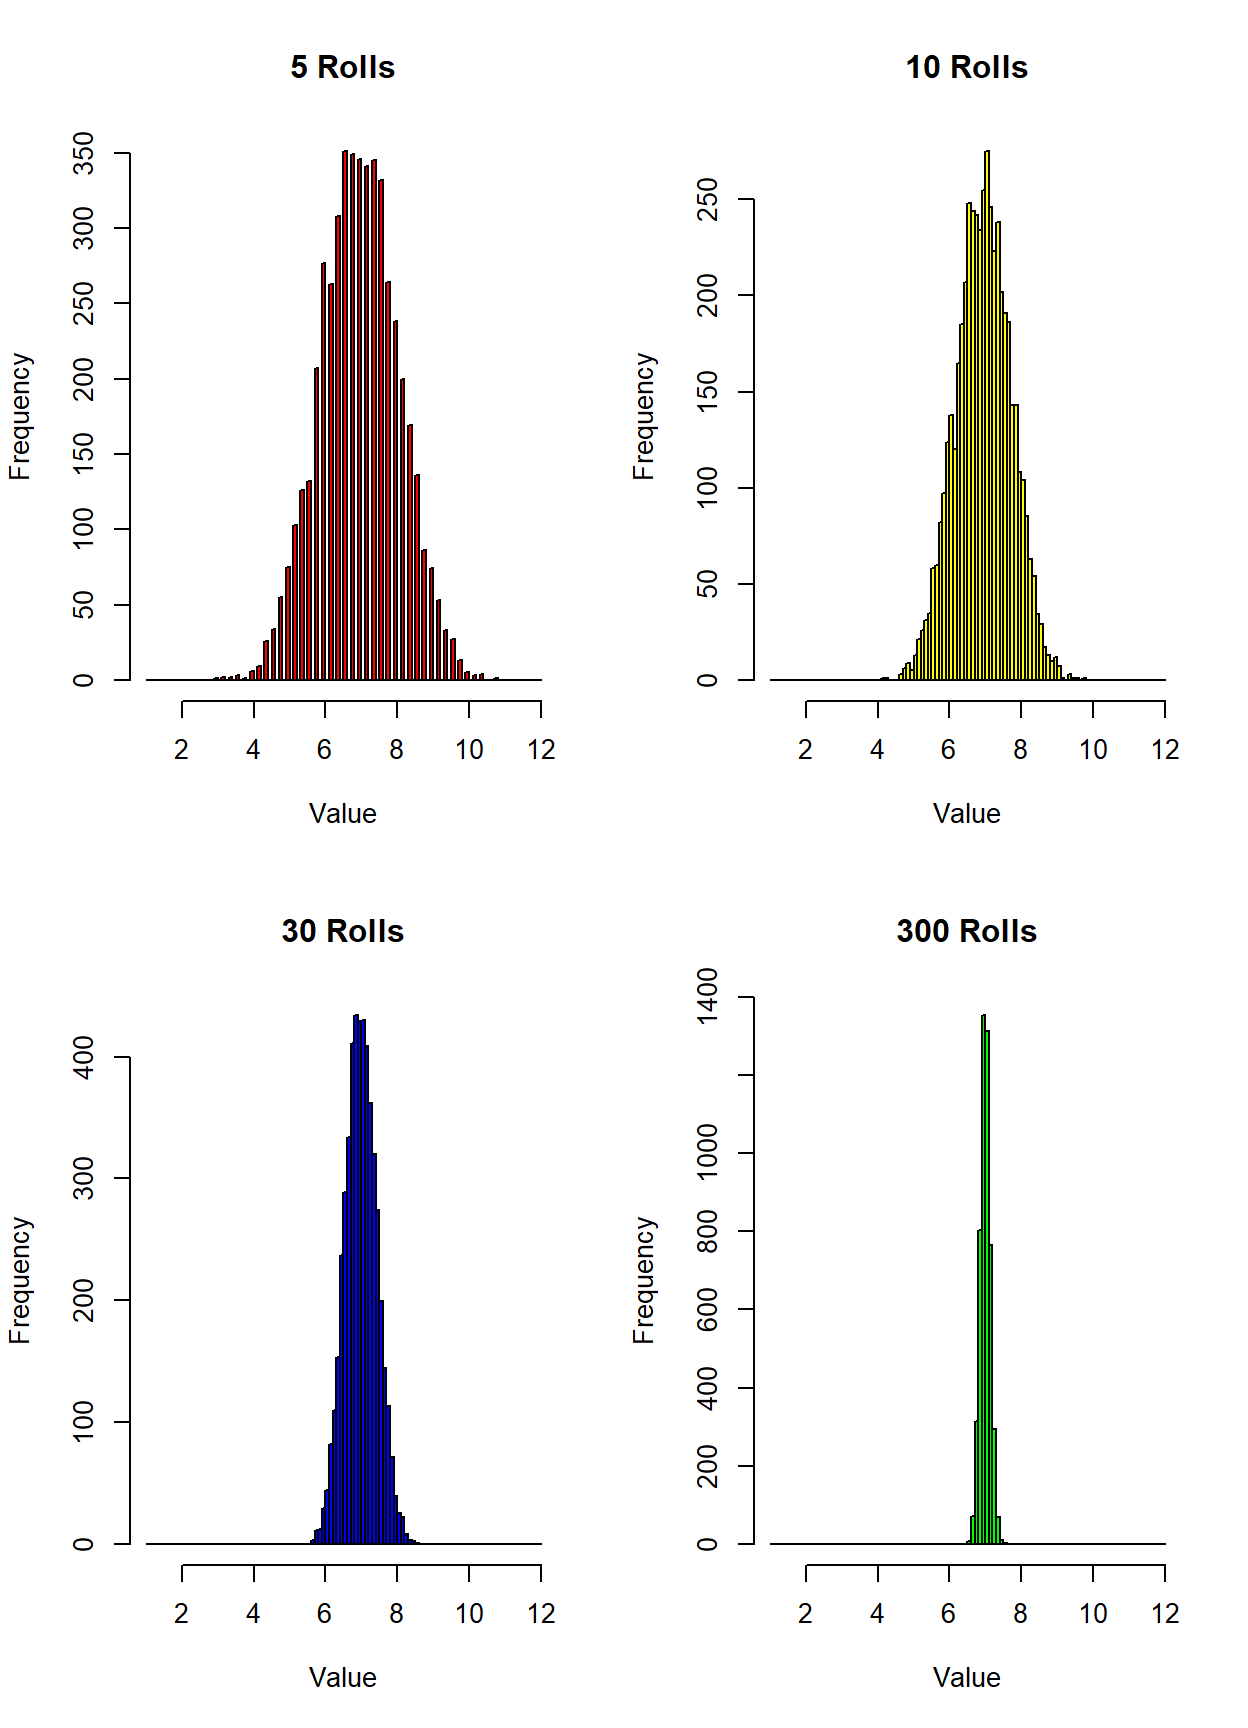
\includegraphics{MBA8350book_files/figure-latex/unnamed-chunk-50-1} 

}

\caption{Sampling Distributions}\label{fig:unnamed-chunk-50}
\end{figure}

The figure is illustrating four potential \emph{sampling distributions}. For example, if you were to collect a sample of 5 rolls, then you would technically be drawing a sample average from the distribution in the upper left. On the other hand, if you decide to roll the dice 300 times, then you are technically drawing a sample average from the distribution in the lower-right.

There are two main takeaways from the above illustration.

\begin{enumerate}
\def\labelenumi{\arabic{enumi}.}
\item
  Sampling distributions \emph{appear} to approximate normal distributions. The normal distribution is the classic \emph{bell-curve} distribution that tends to mysteriously show up in empirical analyses. The CLT is the reason why. Note that even though the original distribution didn't look like a normal distribution at all, you still can construct sampling distributions that appear normal. This holds regardless of the initial population distribution (check out the video about rabbits and dragons on the course website if you don't believe me).
\item
  Sampling distributions become \emph{more} normal and have a lower standard deviation when the sample size gets bigger. Notice that as the sample size goes up, the distributions become narrower. This means that when there is a big sample size there is a very low probability that your going to see sample averages near 2 or 12. This should make sense: If you roll two dice 300 times and take the average, there is no way you are going to record a sample average of 2 unless you roll \emph{snake eyes} 300 times in a row. As the sample size increases, the \emph{extreme} events start getting diluted. This reduces the standard deviation of the sampling distribution.
\item
  The sampling distributions (for \(n \geq 30\)) are distributed normal with mean \(\mu\) and standard deviation \(\sigma / \sqrt{n}\). Technically this means that your random sample will produce a random outcome (a sample mean) which we denote \(\bar{X}\).
\end{enumerate}

\[ \bar{X} \sim N \left( \mu, \frac{\sigma}{\sqrt{n}} \right) \]

You can see these two properties in the four sampling distributions illustrated above. All four sampling distributions are centered around 7, which is the population mean. As sample size gets larger, the sampling distributions get \emph{narrower} around the population mean. This illustrates why a larger sample has a better shot at becoming a better representation of the population.

\hypertarget{application-2-a-sampling-distribution-with-an-unknown-population}{%
\section{Application 2: A Sampling Distribution with an Unknown Population}\label{application-2-a-sampling-distribution-with-an-unknown-population}}

In most applications, we will not be as lucky as in the first application and we will know nothing about the underlying population. We won't know the distributional properties of the population, we won't know any of the population parameters\ldots{} nothing. The beauty of the CLT is that this doesn't matter. We can still apply the CLT to set the stage for statistical inference.

In light of school closings back in 2020, the city of Philadelphia considered sending out \$100 EBT cards to every student registered in public school.

A key question at the beginning of deliberation is how much would this policy cost?

\begin{itemize}
\item
  There are 352,272 families in Philadelphia, and the city has records on how many students are registered in public schools.

  \begin{itemize}
  \tightlist
  \item
    Suppose it is too costly (at the initial stage) to determine the total number of children.
  \end{itemize}
\item
  If we knew the average number of children registered per family, we can get an estimate of the cost of the policy.
\end{itemize}

Suppose we are \emph{omniscient}\ldots{}

\begin{itemize}
\tightlist
\item
  The \textbf{POPULATION} average number of children per family is\ldots{}
  \[\mu = 1.5\]
  \[\sigma = 1.38\]
\end{itemize}

\textbf{NOTE:} We do not know these population parameters. I am simply stating them here so we can refer to them later for verification. In reality, we will \textbf{never} know these population parameters. That's why we need inferential statistics.

\begin{center}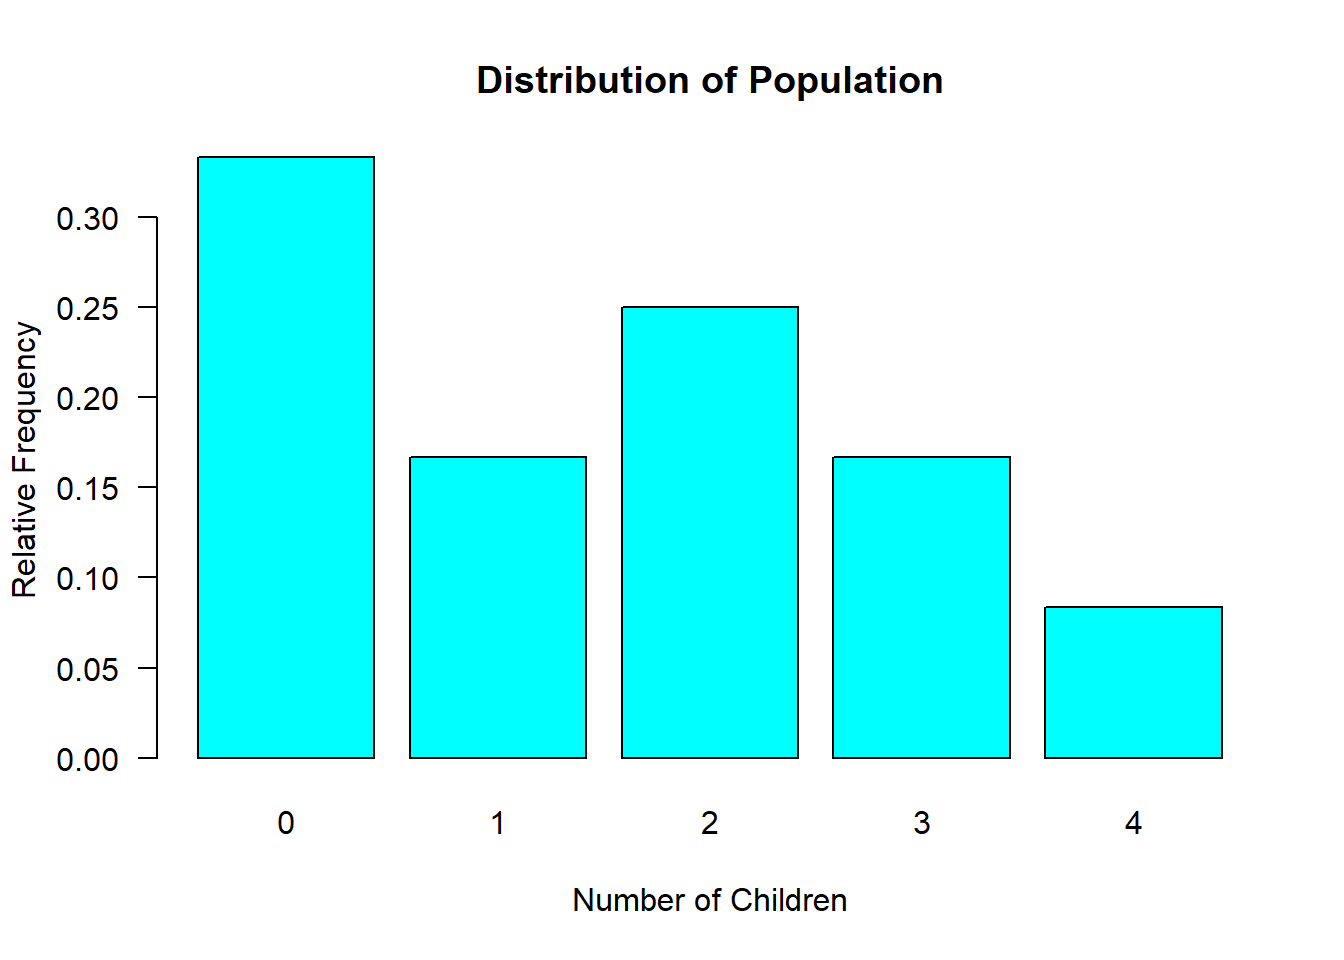
\includegraphics{MBA8350book_files/figure-latex/unnamed-chunk-51-1} \end{center}

\hypertarget{the-sample}{%
\subsection{The Sample}\label{the-sample}}

\begin{itemize}
\item
  Since it is too costly to examine the entire population (at the initial stage), we draw a single sample.
\item
  We use the sample to calculate sample statistics
\item
  Since the sample is randomly drawn from the population, the sample statistics are randomly drawn from a sampling distribution.
\end{itemize}

The characteristics of the sampling distribution depends on the sample size \(n\).

\begin{center}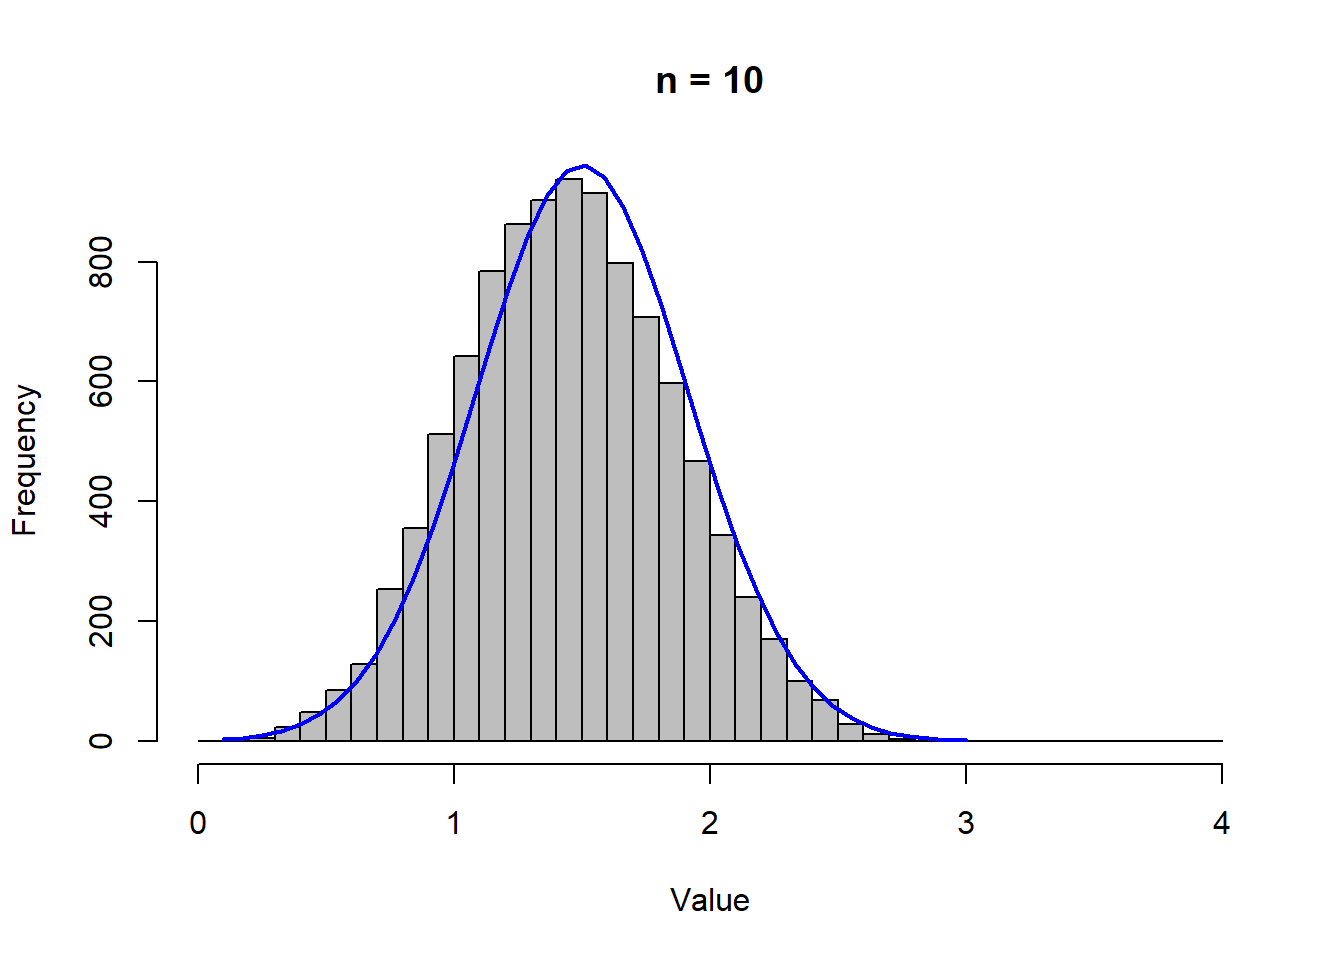
\includegraphics{MBA8350book_files/figure-latex/unnamed-chunk-52-1} \end{center}

\begin{center}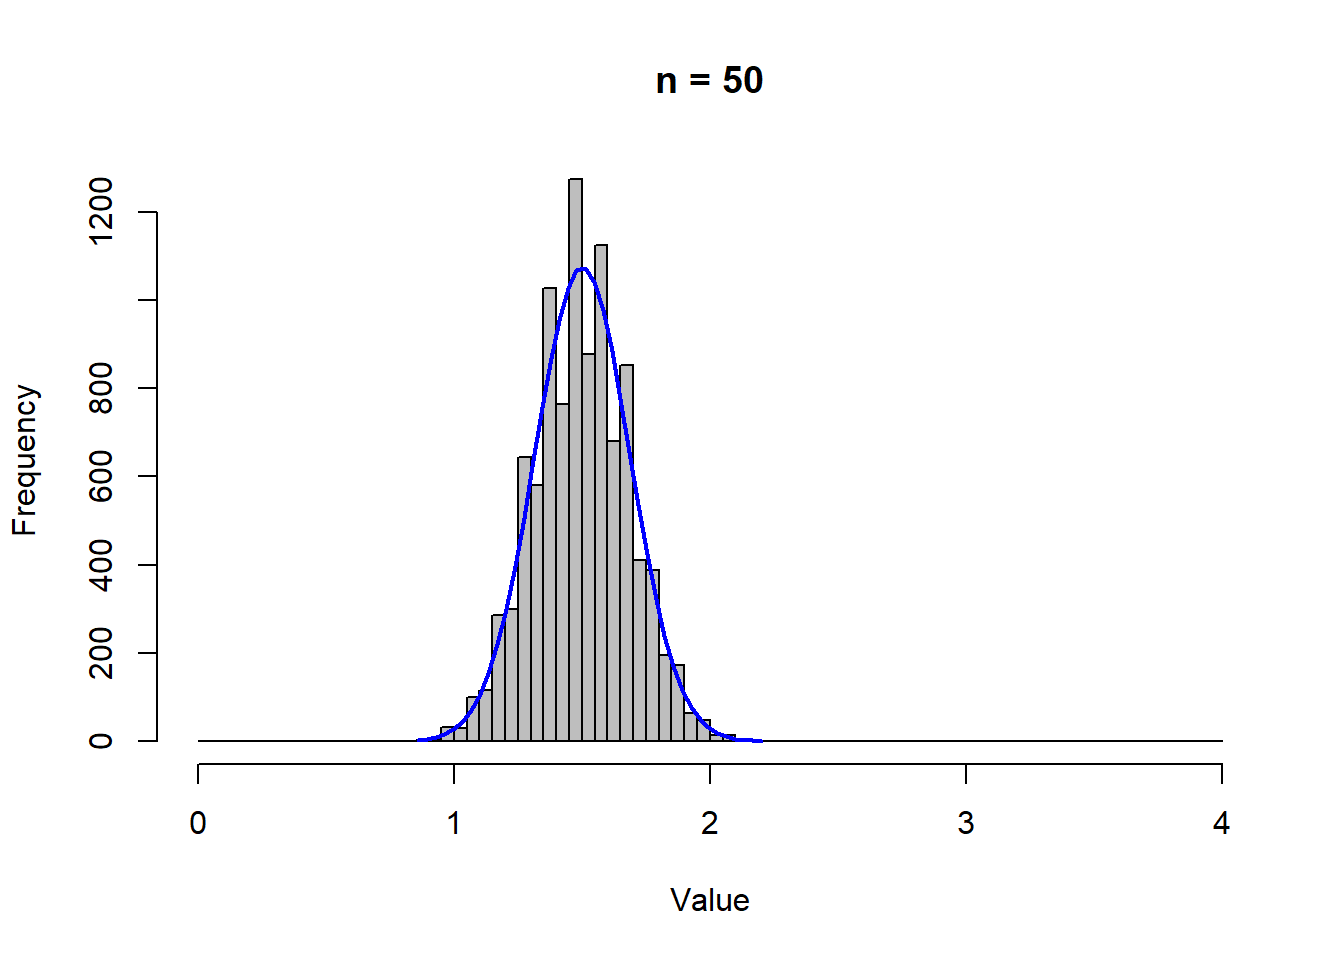
\includegraphics{MBA8350book_files/figure-latex/unnamed-chunk-53-1} \end{center}

\begin{center}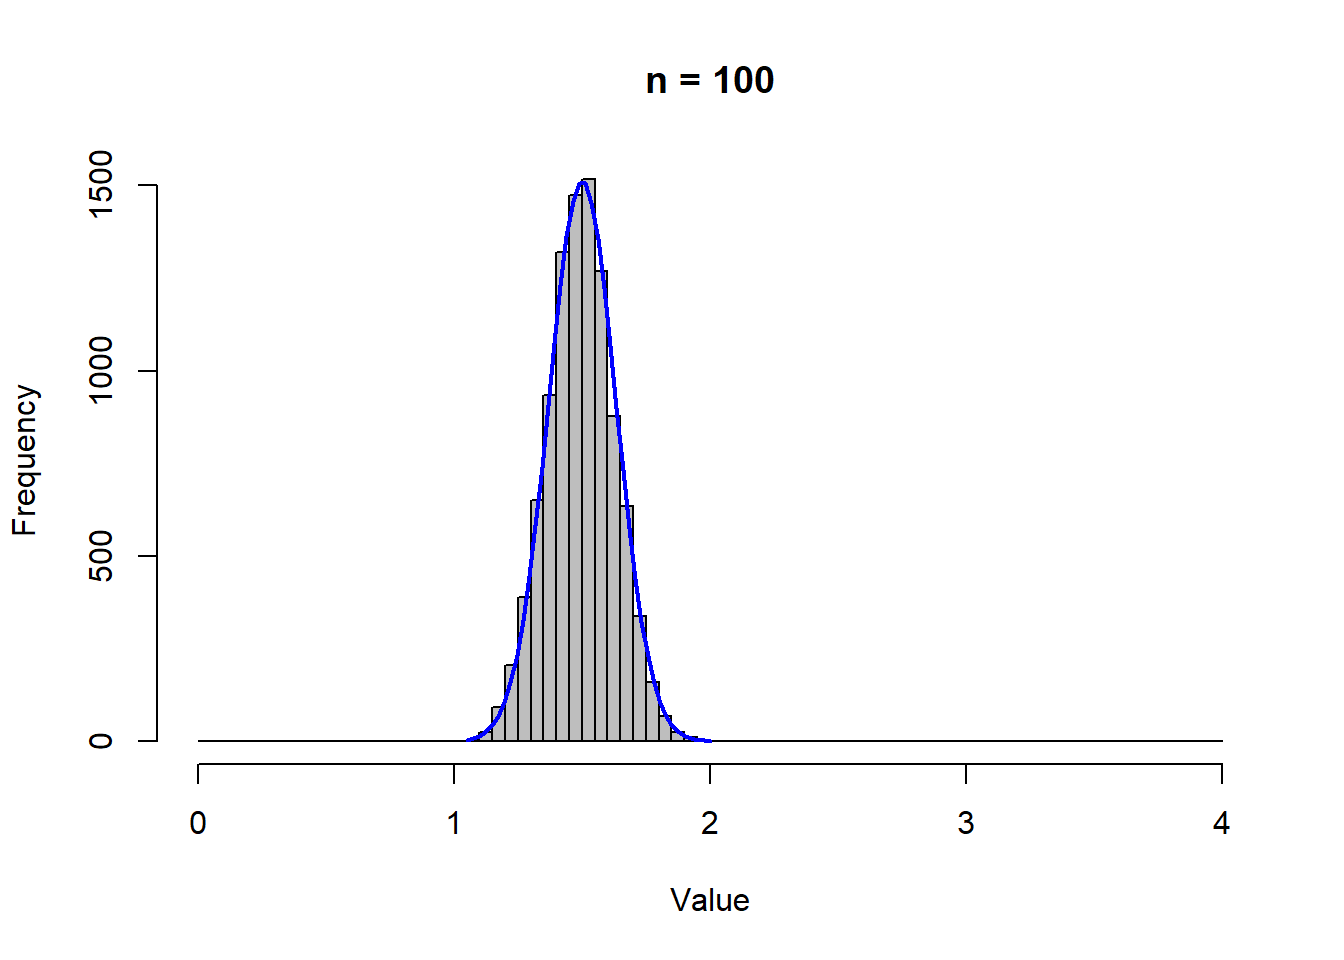
\includegraphics{MBA8350book_files/figure-latex/unnamed-chunk-54-1} \end{center}

The figures above show sampling distributions of various sample sizes. Note that all of these distributions are centered around the same number (of 1.5), and the dispersion around the mean is getting smaller as \(n\) is getting larger. In other words, the standard deviation \(\sigma / \sqrt{n}\) is getting smaller because \(n\) is getting larger (while \(\sigma\) remains unchanged).

\hypertarget{the-punchline-1}{%
\section{The Punchline}\label{the-punchline-1}}

Once you determine a sample size \((n)\), you get \textbf{one random draw} from the appropriate sampling distribution.

\begin{itemize}
\item
  The distribution is approximately \emph{normal}
\item
  The mean is \(\mu\)
\item
  The standard deviation \(\sigma/\sqrt{n}\)
\end{itemize}

What does this buy us? The answer is \emph{everything} if we want to apply any form of \emph{confidence} (i.e., stating a probability of occurring).

The reason is that the normal distribution has a lot of useful properties.

\begin{enumerate}
\def\labelenumi{\arabic{enumi}.}
\item
  The distribution is symmetric. The shape of the distribution to the right of the mean is identical to the shape of the distribution to the left of the mean.
\item
  Approximately 95\% of all possible outcomes are within 2 standard deviations of the mean.
\end{enumerate}

To illustrate these two properties, consider the generic normal distribution illustrated below. You can easily see the symmetry of the distribution, while the shaded area represents 95\% of the distribution. In probability terms, 95\% of the area of the probability distribution means that there is a 95\% chance of drawing a value within this range.

\begin{center}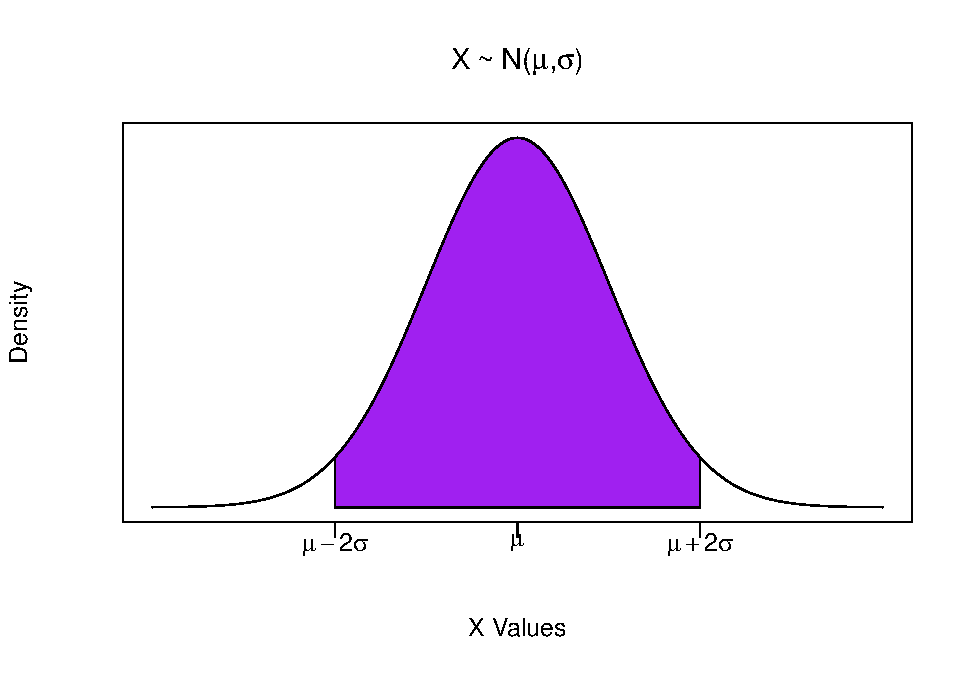
\includegraphics{MBA8350book_files/figure-latex/unnamed-chunk-55-1} \end{center}

So what does this really buy us? Consider the application above about the Philadelphia policy where we would have in reality have no idea what the population parameters \((\mu,\;\sigma)\) are, or what the population distribution even looks like. However, the CLT says that if we decide on a sample size \(n\), then we will draw from a sampling distribution that is a normal distribution with mean \(mu\) and standard deviation \(\sigma / \sqrt{n}\).

\begin{center}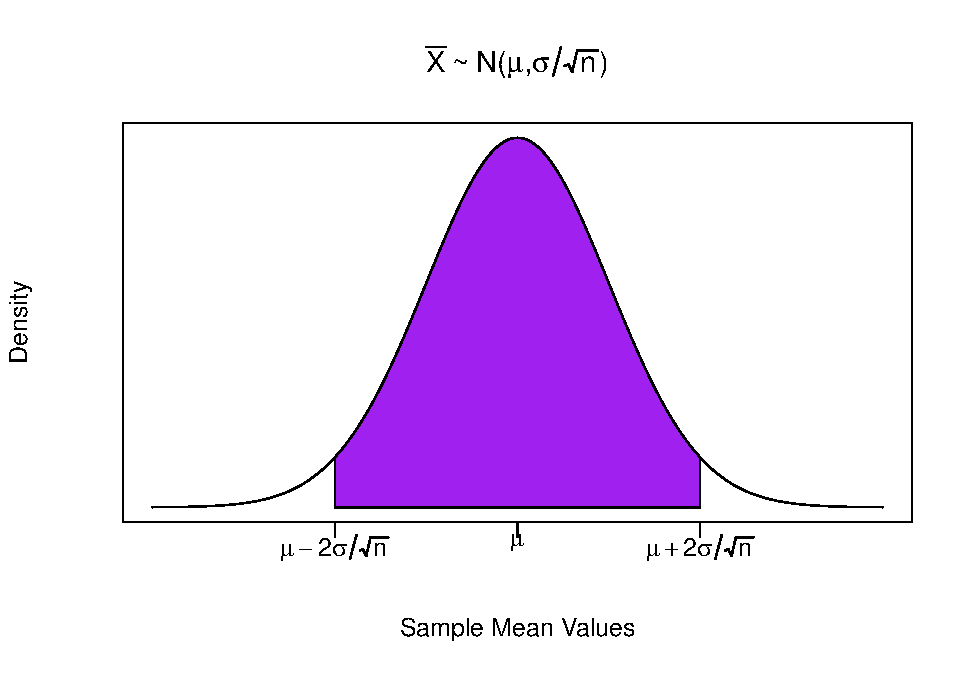
\includegraphics{MBA8350book_files/figure-latex/unnamed-chunk-56-1} \end{center}

So what we know is that once we draw a random sample and construct a sample mean, we can say with 95\% confidence that that sample mean was drawn from the shaded region of the above distribution. We know what the sample mean value is because we just calculated it. What we don't know is what \(/mu\) is. However, we can construct a probabilistic range (a \emph{confidence interval}) around where we think this population parameter lies. This is where we are going next.

\hypertarget{CI}{%
\chapter{Confidence Intervals}\label{CI}}

With the concept of the Central Limit Theorem (CLT) under our belts, we can discuss our first application of statistical inference. The main concept is that when a statistician discusses \emph{confidence}, they are actually saying how likely something is going to happen. In other words, 95\% confidence in a statement means that something is going to happen 95 out of 100 replications. We only get one shot (not 100 replications), so it is the likelihood that it's going to happen in this one shot.

In order for us to get into statistical inference, we need to first have a refresher on probability. Thanks to the CLT, our probability calculations are going to come from the normal probability distribution.

\hypertarget{a-refresher-on-probability}{%
\section{A Refresher on Probability}\label{a-refresher-on-probability}}

Suppose I give you a random variable \((X)\) and tell you that this random variable comprises a normal distribution with an \emph{arbitrary} mean equal to \(\mu\) and an \emph{arbitrary} standard deviation equal to \(\sigma\). We can denote this generally as \(X \sim N(\mu,\sigma)\) and we can draw this generally as

\begin{center}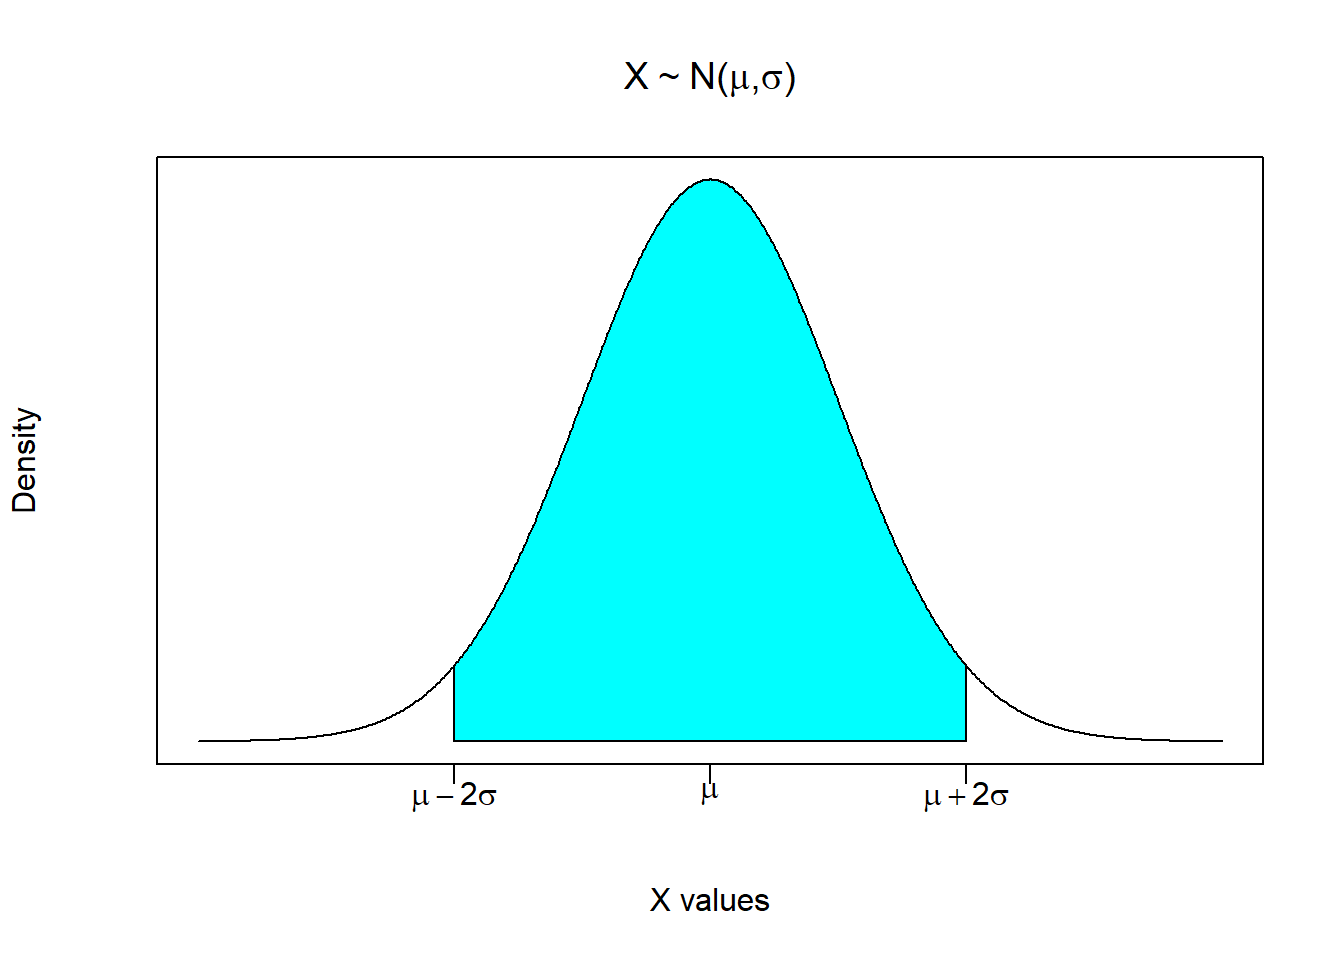
\includegraphics{MBA8350book_files/figure-latex/unnamed-chunk-58-1} \end{center}

This picture is the normal probability density of this random variable. It is very much like a histogram, only we can consider a continuum of possible numbers (i.e., unlimited number of histogram bins). A normal probability density has several useful properties.

\begin{enumerate}
\def\labelenumi{\arabic{enumi}.}
\item
  It is centered at the mean. It is a \textbf{symmetric} distribution with 50\% of the probability being on either side of the mean.
\item
  Like all probability distributions, it must add up to 1 (or 100\%). This is like saying that the probability of reaching into a hat full of numbers and pulling out a number between positive and negative infinity is equal to 100\%.
\item
  A normal distribution has the nice property that approximately 95\% of the density area is between two standard deviation above and below the mean. This is the shaded area in the above figure. It roughly states that if you reached into a bowl full of numbers that comprised this distribution, then you have a 95\% chance of pulling out a number between \(\mu-2\sigma\) and \(\mu+2\sigma\).
\end{enumerate}

This is very useful, but for our purposes we need to take this arbitrary normal distribution and transform it into a \textbf{standard normal distribution}. We do this by applying what is known as a Z-transformation:

\[Z=\frac{X-\mu}{\sigma}\]

The figure below illustrates how this transformation changes an otherwise arbitrary normal distribution. The top figure is the arbitrary random variable with a mean of \(\mu\) and a standard deviation of \(\sigma\) \((X \sim N(\mu,\sigma))\). The second figure shows what happens to the distribution when we subtract the mean from every number in the distribution. This effectively shifts the distribution such that it is now centered around zero, so we now have a normally distributed random variable with a mean of zero and a standard deviation of \(\sigma\) \((X-\mu \sim N(0,\sigma))\). The third figure shows what happens when we divide every number in the distribution by \(\sigma\). Recall that \(\sigma\) is a positive number that can be greater or less than one. If you divide a number by a number less than one then the number gets bigger. If you divide a number by a number greater than one then the number gets smaller. This means that dividing every number by \(\sigma\) will either increase or decrease the dispersion of values such that the standard deviation is equal to one. A normally distributed random variable with a mean of zero and a standard deviation is said to be a standard normal random variable \((Z \sim N(0,1))\).

Note that this transformation shifts the distribution, but \textbf{does not} change its properties. This was done on purpose to get you to see that a standard normal transformation shifts the mean and alters the dispersion, but does not change the facts that the distribution is still symmetric, still adds to one, and still has the property that 95\% of the probability area is between 2 standard deviations to the right and left of the mean.

\begin{center}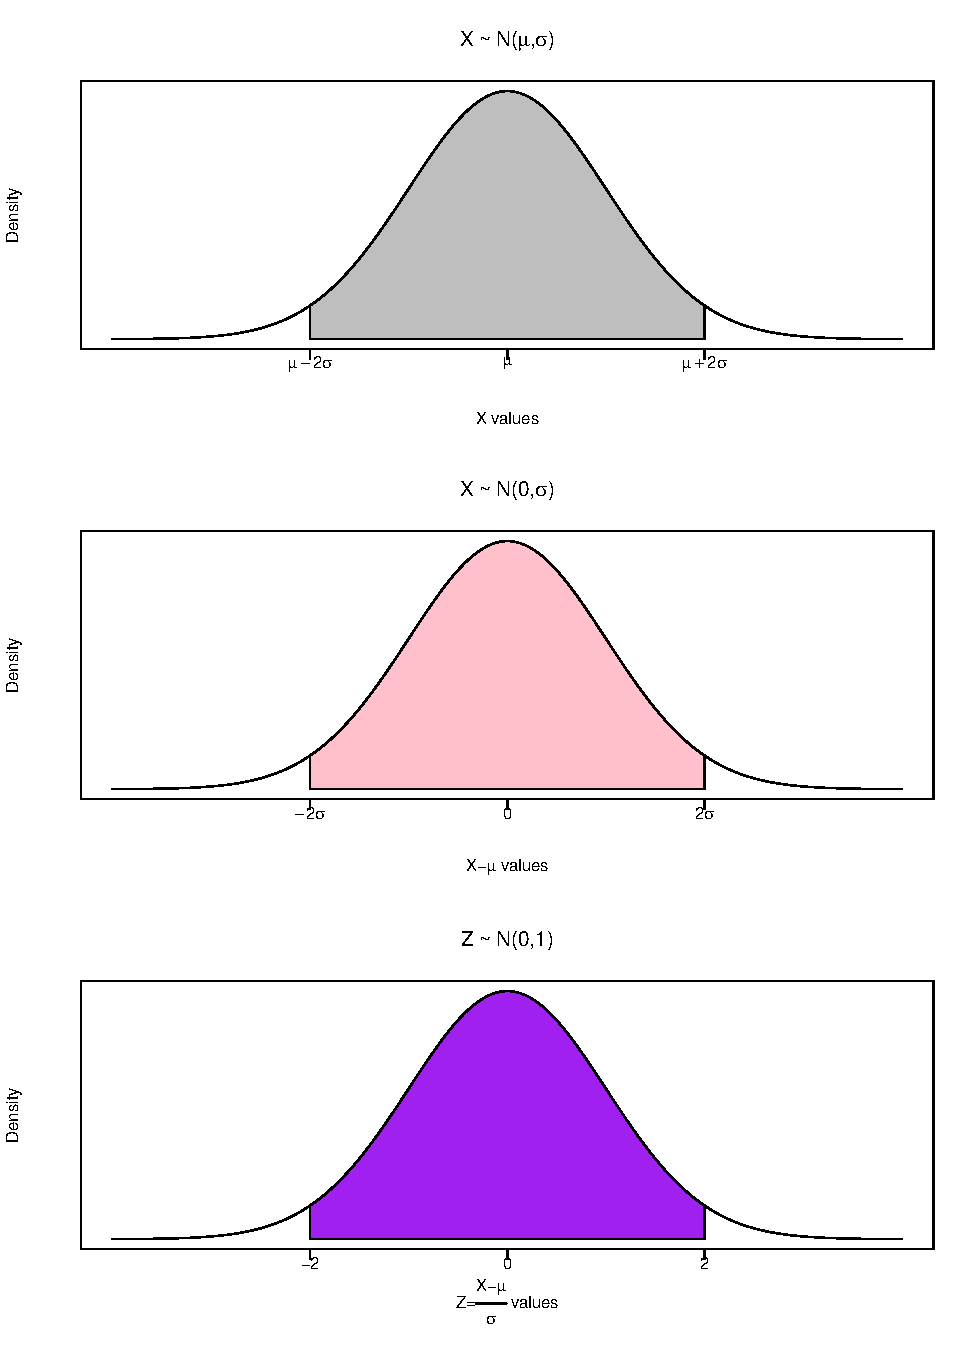
\includegraphics{MBA8350book_files/figure-latex/unnamed-chunk-59-1} \end{center}

\emph{What does this transformation do?} It takes a normally distributed random variable with arbitrary \(\mu\) and \(\sigma\), and transforms the distribution into one with mean 0 and standard deviation 1.

\emph{Why is this useful?} It can easily be used for numerical probability calculations - but this isn't as useful nowadays since we have computers. However, this transformation will be essential to put the normal distribution on the same level as other distributions we will soon encounter.

\hypertarget{application-1}{%
\subsection{Application 1}\label{application-1}}

Suppose there exists a bowl of numbered cards. The numbers on these cards comprises a normal distribution where the mean value is 5, and the standard deviation is 3.
\[X \sim N(5,3)\]

We now have everything we need to calculate the probability of any outcome from this data-generating process. For example, suppose we wanted to determine the probability of reaching into this bowl and picking a number between 2 and 3. In probability terms:

\[Pr(2 \leq x \leq 3)\]

\begin{enumerate}
\def\labelenumi{\arabic{enumi}.}
\tightlist
\item
  First we perform a standard normal transformation \(Z=\frac{X-\mu}{\sigma}=\frac{X-5}{3}\), so our probability question gets transformed as well:
\end{enumerate}

\[Pr(2 \leq x \leq 3)=Pr\left(\frac{2-5}{3} \leq \frac{x-5}{3} \leq \frac{3-5}{3}\right)\]

This delivers the same probability question, only in standard normal terms:

\[Pr(2 \leq x \leq 3)=Pr\left(-1 \leq z \leq -\frac{2}{3}\right)\]

\begin{enumerate}
\def\labelenumi{\arabic{enumi}.}
\setcounter{enumi}{1}
\tightlist
\item
  Next we illustrate exactly what this probability question looks like in our distribution. In other words, indicate what \emph{slice} of the distribution answers the probability question. This slice is illustrated in the figure below by shading in the probability area of the distribution between -1 and \(-\frac{2}{3}\).
\end{enumerate}

\begin{center}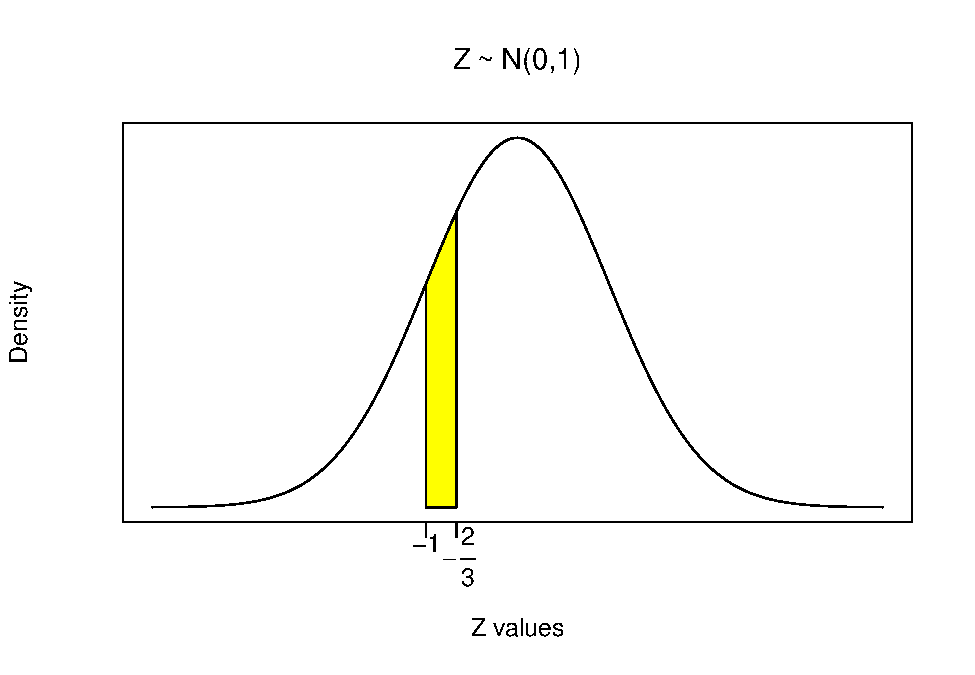
\includegraphics{MBA8350book_files/figure-latex/unnamed-chunk-60-1} \end{center}

\begin{enumerate}
\def\labelenumi{\arabic{enumi}.}
\setcounter{enumi}{2}
\tightlist
\item
  Finally, we calculate the probability in R. Now this is where the illustration above will help get us organized, because we can exploit the distributional properties of symmetry and the distribution summing to one. This is important because we can use R to calculate the same number in several different ways. All of these routes to the answer are acceptable, so we will go through them all here.
\end{enumerate}

First thing to do is introduce you to the R command ``pnorm''

\begin{verbatim}
pnorm(q, mean = 0, sd = 1, lower.tail = TRUE)
\end{verbatim}

The command requires a number (\emph{quantity}) for the variable q. It will then use a normal distribution with a mean of 0 and a standard error of 1 (\emph{by default}) and calculate the area to the \textbf{left of the number q}. Note that this is the default action which is given by ``lower.tail = TRUE''. If you want to turn off this default action, then you need to set ``lower.tail = FALSE'' and the command will calculate the area to the \textbf{right of the number q}. For example, we can calculate \(Pr(z\leq-1)\) or the area to the left of -1.

\begin{Shaded}
\begin{Highlighting}[]
\FunctionTok{pnorm}\NormalTok{(}\SpecialCharTok{{-}}\DecValTok{1}\NormalTok{)}
\end{Highlighting}
\end{Shaded}

\begin{verbatim}
## [1] 0.1586553
\end{verbatim}

We could also calculate \(Pr(z\geq-1)\) or the area to the right of -1.

\begin{Shaded}
\begin{Highlighting}[]
\FunctionTok{pnorm}\NormalTok{(}\SpecialCharTok{{-}}\DecValTok{1}\NormalTok{,}\AttributeTok{lower.tail =} \ConstantTok{FALSE}\NormalTok{)}
\end{Highlighting}
\end{Shaded}

\begin{verbatim}
## [1] 0.8413447
\end{verbatim}

These two probability areas sum to 1 (as they should), and are illustrated below. The left figure illustrates that 15.9\% of the area under the distribution is to the left of -1, so you have a 15.9\% chance of picking a number less than or equal to -1. Conversely, the right figure illustrates that 84.1\% of the area under the distribution is to the right of -1, so you have a 84.1\% chance of picking a number greater than or equal to -1.

\begin{center}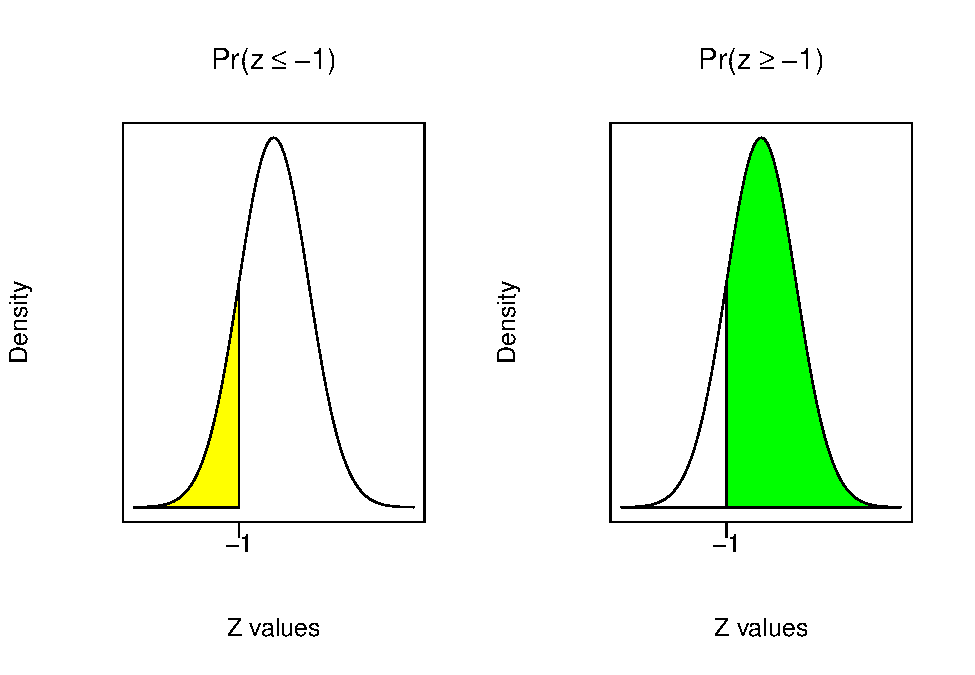
\includegraphics{MBA8350book_files/figure-latex/unnamed-chunk-63-1} \end{center}

Now that we know how R likes to calculate probabilities, we can use it to determine \(Pr(-1 \leq z \leq -\frac{2}{3})\) which is the shaded slice of the distribution in the previous figure.

\begin{enumerate}
\def\labelenumi{\arabic{enumi}.}
\tightlist
\item
  Using the \emph{default} setting: suppose you want to calculate all of the probabilities using the default setting of calculating areas to the left. The shaded slice of the distribution is then the difference between the area to the left of \(-\frac{2}{3}\) and the area to the left of -1.
\end{enumerate}

\[Pr\left(-1 \leq z \leq -\frac{2}{3}\right)=Pr\left(z \leq -\frac{2}{3}\right) - Pr\left(z \leq -1\right)\]

\begin{Shaded}
\begin{Highlighting}[]
\FunctionTok{pnorm}\NormalTok{(}\SpecialCharTok{{-}}\DecValTok{2}\SpecialCharTok{/}\DecValTok{3}\NormalTok{)}\SpecialCharTok{{-}}\FunctionTok{pnorm}\NormalTok{(}\SpecialCharTok{{-}}\DecValTok{1}\NormalTok{)}
\end{Highlighting}
\end{Shaded}

\begin{verbatim}
## [1] 0.09383728
\end{verbatim}

\begin{enumerate}
\def\labelenumi{\arabic{enumi}.}
\setcounter{enumi}{1}
\tightlist
\item
  Removing the \emph{default} setting. If you want to calculate probabilities from the right (which might come in handy), then the same slice of the distribution is the difference between the area to the right of \(-1\) and the area to the right of \(-\frac{2}{3}\).
\end{enumerate}

\[Pr\left(-1 \leq z \leq -\frac{2}{3}\right)=Pr(z \geq -1) - Pr\left(z \geq -\frac{2}{3}\right)\]

\begin{Shaded}
\begin{Highlighting}[]
\FunctionTok{pnorm}\NormalTok{(}\SpecialCharTok{{-}}\DecValTok{1}\NormalTok{,}\AttributeTok{lower.tail =} \ConstantTok{FALSE}\NormalTok{)}\SpecialCharTok{{-}}\FunctionTok{pnorm}\NormalTok{(}\SpecialCharTok{{-}}\DecValTok{2}\SpecialCharTok{/}\DecValTok{3}\NormalTok{,}\AttributeTok{lower.tail =} \ConstantTok{FALSE}\NormalTok{)}
\end{Highlighting}
\end{Shaded}

\begin{verbatim}
## [1] 0.09383728
\end{verbatim}

\begin{enumerate}
\def\labelenumi{\arabic{enumi}.}
\setcounter{enumi}{2}
\tightlist
\item
  Exploiting that the area sums to 1. Yet another way to arrive at the same answer is to calculate the area to the left of \(-1\), the area to the right of \(-\frac{2}{3}\), and arrive at the slice by subtracting these areas from 1.
\end{enumerate}

\[Pr\left(-1 \leq z \leq -\frac{2}{3}\right)=1 - Pr(z \leq -1) - Pr\left(z \geq -\frac{2}{3}\right)\]

\begin{Shaded}
\begin{Highlighting}[]
\DecValTok{1}\SpecialCharTok{{-}}\FunctionTok{pnorm}\NormalTok{(}\SpecialCharTok{{-}}\DecValTok{1}\NormalTok{)}\SpecialCharTok{{-}}\FunctionTok{pnorm}\NormalTok{(}\SpecialCharTok{{-}}\DecValTok{2}\SpecialCharTok{/}\DecValTok{3}\NormalTok{,}\AttributeTok{lower.tail =} \ConstantTok{FALSE}\NormalTok{)}
\end{Highlighting}
\end{Shaded}

\begin{verbatim}
## [1] 0.09383728
\end{verbatim}

As you can see, each procedure delivers the same answer - you have a 9.4\% chance of picking a number from a standard normal distribution between -1 and \(-\frac{2}{3}\).

Note that this is the same answer to the original question (before we transformed the distribution). The take away from this exercise is that there are plenty of straightforward ways of calculating probabilities in R, and we will be making a fair amount of use of them.

\[Pr\left(-1 \leq z \leq -\frac{2}{3}\right)=0.094\]

\hypertarget{application-2}{%
\subsection{Application 2}\label{application-2}}

Let us look deeper into our dice example. In particular, if I were to roll two fair dice a \(n\) number of times and calculated the average, what range of values should I expect to see?

Recall that the distribution of the population has a mean of 7 and a standard deviation of 2.45. This means that for \(n \geq 30\), the \emph{sampling distribution} is normal and given by

\[\bar{X} \sim N \left( 7, \; \frac{2.45}{\sqrt{n}} \right)\]

Recall that in this (rare) example, we \emph{know} the population parameters. Therefore, we can build a range where we expect sample averages to reside.

\begin{Shaded}
\begin{Highlighting}[]
\NormalTok{X }\OtherTok{\textless{}{-}} \FunctionTok{seq}\NormalTok{(}\SpecialCharTok{{-}}\DecValTok{4}\NormalTok{,}\DecValTok{4}\NormalTok{,}\FloatTok{0.01}\NormalTok{)}
\NormalTok{Y }\OtherTok{\textless{}{-}} \FunctionTok{dnorm}\NormalTok{(X)}

\FunctionTok{plot}\NormalTok{(X,Y,}\AttributeTok{type=}\StringTok{"n"}\NormalTok{,}\AttributeTok{xlab=}\StringTok{"Average Values"}\NormalTok{,}\AttributeTok{ylab =} \StringTok{"Density"}\NormalTok{,}
     \AttributeTok{yaxt =} \StringTok{"n"}\NormalTok{, }\AttributeTok{xaxt =} \StringTok{"n"}\NormalTok{, }\AttributeTok{main =}  \FunctionTok{TeX}\NormalTok{(}\StringTok{\textquotesingle{}$X }\SpecialCharTok{\textbackslash{}\textbackslash{}}\StringTok{sim N(7,2.45 / }\SpecialCharTok{\textbackslash{}\textbackslash{}}\StringTok{sqrt\{n\})\textquotesingle{}}\NormalTok{))}
\NormalTok{xtick}\OtherTok{\textless{}{-}}\FunctionTok{seq}\NormalTok{(}\SpecialCharTok{{-}}\DecValTok{2}\NormalTok{, }\DecValTok{2}\NormalTok{, }\AttributeTok{by=}\DecValTok{2}\NormalTok{)}
\FunctionTok{axis}\NormalTok{(}\AttributeTok{side=}\DecValTok{1}\NormalTok{, }\AttributeTok{at=}\NormalTok{xtick, }\AttributeTok{labels =} \ConstantTok{FALSE}\NormalTok{)}
\FunctionTok{text}\NormalTok{(}\AttributeTok{x=}\NormalTok{xtick, }\FunctionTok{par}\NormalTok{(}\StringTok{"usr"}\NormalTok{)[}\DecValTok{3}\NormalTok{],  }
     \AttributeTok{labels =} \FunctionTok{c}\NormalTok{(}\FunctionTok{TeX}\NormalTok{(}\StringTok{\textquotesingle{}$7{-}1.96}\SpecialCharTok{\textbackslash{}\textbackslash{}}\StringTok{frac\{2.45\}\{}\SpecialCharTok{\textbackslash{}\textbackslash{}}\StringTok{sqrt\{n\}\}$\textquotesingle{}}\NormalTok{),}\DecValTok{7}\NormalTok{, }
                \FunctionTok{TeX}\NormalTok{(}\StringTok{\textquotesingle{}$7+1.96}\SpecialCharTok{\textbackslash{}\textbackslash{}}\StringTok{frac\{2.45\}\{}\SpecialCharTok{\textbackslash{}\textbackslash{}}\StringTok{sqrt\{n\}\}$\textquotesingle{}}\NormalTok{)), }
     \AttributeTok{pos =} \DecValTok{1}\NormalTok{, }\AttributeTok{xpd =} \ConstantTok{TRUE}\NormalTok{)}
\NormalTok{i }\OtherTok{\textless{}{-}}\NormalTok{ X }\SpecialCharTok{\textgreater{}=} \SpecialCharTok{{-}}\DecValTok{2} \SpecialCharTok{\&}\NormalTok{ X }\SpecialCharTok{\textless{}=} \DecValTok{2}
\FunctionTok{lines}\NormalTok{(X, Y)}
\FunctionTok{polygon}\NormalTok{(}\FunctionTok{c}\NormalTok{(}\SpecialCharTok{{-}}\DecValTok{2}\NormalTok{,X[i],}\DecValTok{2}\NormalTok{), }\FunctionTok{c}\NormalTok{(}\DecValTok{0}\NormalTok{,Y[i],}\DecValTok{0}\NormalTok{), }\AttributeTok{col=}\StringTok{"purple"}\NormalTok{)}
\end{Highlighting}
\end{Shaded}

\begin{center}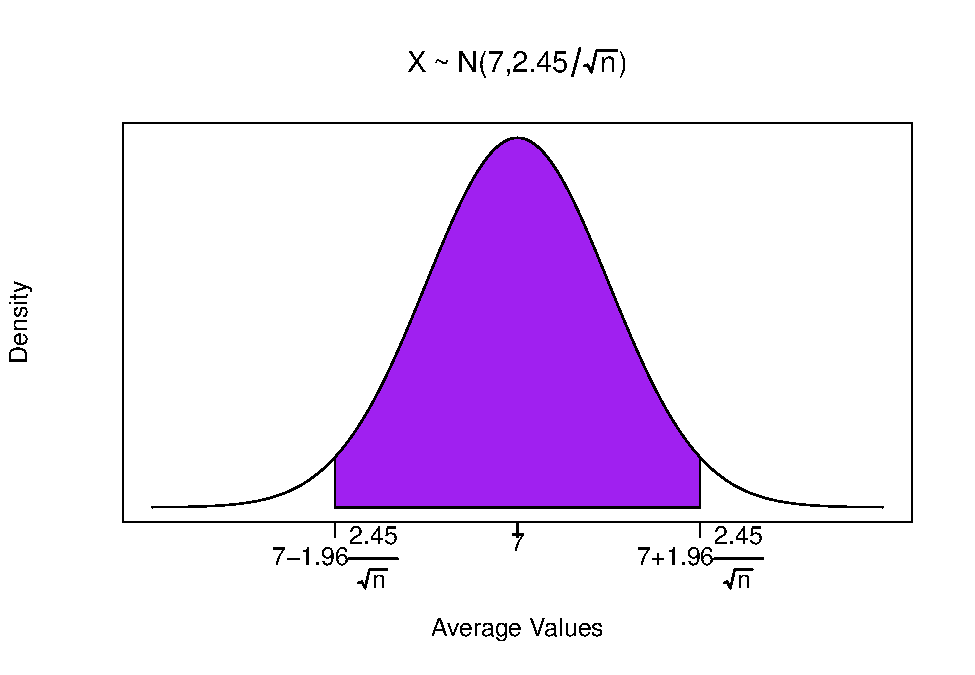
\includegraphics{MBA8350book_files/figure-latex/unnamed-chunk-67-1} \end{center}

So if we collected a sample on \(n=100\), meaning we rolled two dice 100 times, recorded the total each time, and calculated the mean value, then\ldots{}

\[Pr\left( 7-1.96 \frac{2.45}{\sqrt{100}} \leq \bar{X} \leq 7-1.96 \frac{2.45}{\sqrt{100}} \right) = 0.95\]

\begin{Shaded}
\begin{Highlighting}[]
\NormalTok{Z }\OtherTok{=} \FunctionTok{qnorm}\NormalTok{(}\FloatTok{0.975}\NormalTok{,}\AttributeTok{lower.tail =} \ConstantTok{FALSE}\NormalTok{)}
\NormalTok{n }\OtherTok{=} \DecValTok{100}
\NormalTok{mu }\OtherTok{=} \DecValTok{7}
\NormalTok{sigma }\OtherTok{=} \FloatTok{2.45}

\NormalTok{(}\AttributeTok{LFT =}\NormalTok{ mu }\SpecialCharTok{{-}}\NormalTok{ Z }\SpecialCharTok{*}\NormalTok{ sigma }\SpecialCharTok{/} \FunctionTok{sqrt}\NormalTok{(n))}
\end{Highlighting}
\end{Shaded}

\begin{verbatim}
## [1] 7.480191
\end{verbatim}

\begin{Shaded}
\begin{Highlighting}[]
\NormalTok{(}\AttributeTok{RHT =}\NormalTok{ mu }\SpecialCharTok{+}\NormalTok{ Z }\SpecialCharTok{*}\NormalTok{ sigma }\SpecialCharTok{/} \FunctionTok{sqrt}\NormalTok{(n))}
\end{Highlighting}
\end{Shaded}

\begin{verbatim}
## [1] 6.519809
\end{verbatim}

\[Pr(6.52 \leq \bar{X} \leq 7.48) = 0.95\]

This means that with 95\% confidence, the single outcome from your \emph{experiment} will be within 6.52 and 7.48 if the die you are rolling are in fact fair.\footnote{Note that the code used a command called \emph{qnorm}. This gets described further below.}

As stated earlier, this example is rare because we know the population parameters. When we don't, we reverse engineer the probability statement so we can take what we know (the sample statistics) and use them to say something about what we don't. This is known as a confidence interval.

\hypertarget{deriving-a-confidence-interval}{%
\section{Deriving a Confidence Interval}\label{deriving-a-confidence-interval}}

Recall when we randomly draw a sample from a sampling distribution and use it to calculate a sample mean \((\bar{X})\), we essentially state that a sample mean is a random variable. Since the CLT states that the sampling distribution is a normal distribution, then this further states that the sample mean is a normally distributed random variable with a mean of \(\mu\) and a standard deviation of \(\frac{\sigma}{\sqrt{n}}\).

\[\bar{X} \sim N\left(\mu,\frac{\sigma}{\sqrt{n}}\right)\]

We can apply our standardization trick so we have

\[Z=\frac{\bar{X}-\mu}{(\sigma/\sqrt{n})}\]

Suppose we have a sample of size \(n\), calculated a sample mean \(\bar{X}\), and that we \emph{know} the population standard deviation \(\sigma\) (more on this later). If we know these values, then we can use the standard normal distribution as well as the normalization above to draw statistical inference on the population parameter \(\mu\).

\emph{What can we say about} \(\mu\)?

\begin{itemize}
\item
  Since our sample has the same characteristics as the population, we would like to say \(\mu = \bar{X}\) (i.e., \(Z=0\)), but this is not likely. Recall the dice example discussed earlier, while 7 (the population mean) is the most likely average of a sample, there is a larger likelihood of a sample average \emph{close} to, but not exactly equal to the population mean.
\item
  Since \(\bar{X}\) is a single draw from a normal distribution, we can construct a \emph{probabilistic} range around \(\mu\). This range requires an arbitrary level of confidence \((1-\alpha)\) - which provides bounds for the Z distribution (i.e., it gives us the area under the curve).
\end{itemize}

We therefore start with a probabilistic statement using a standard normal distribution:

\[Pr\left(-Z \leq \frac{\bar{X}-\mu}{(\sigma/\sqrt{n})} \leq Z\right)=1-\alpha\]

This states (in general terms) that the probability of realizing a value of \(\frac{\bar{X}-\mu}{(\sigma/\sqrt{n})}\) drawn from a standard normal distributed random variable to be between the values -Z and Z is equal to \(1-\alpha\). To put this into context, suppose I set \(\alpha=0.05\) so \(1-\alpha=0.95\) implies that I am looking for something that will occur with 95\% probability. Recall the normal distribution has the nice property that 95\% of the probability space is approximately between two standard deviations above and below the mean. By approximately, I mean it is actually 1.96 and not 2.\footnote{This explains the 1.96 used in the dice application above.}

Finding these numbers requires another R command: qnorm.

\begin{verbatim}
qnorm(p, mean = 0, sd = 1, lower.tail = TRUE)
\end{verbatim}

Just like how pnorm takes a quantity and returns a probability, qnorm takes a probability and returns a quantity.

\begin{Shaded}
\begin{Highlighting}[]
\FunctionTok{qnorm}\NormalTok{(}\FloatTok{0.025}\NormalTok{)}
\end{Highlighting}
\end{Shaded}

\begin{verbatim}
## [1] -1.959964
\end{verbatim}

\begin{Shaded}
\begin{Highlighting}[]
\FunctionTok{qnorm}\NormalTok{(}\FloatTok{0.975}\NormalTok{,}\AttributeTok{lower.tail=}\ConstantTok{FALSE}\NormalTok{)}
\end{Highlighting}
\end{Shaded}

\begin{verbatim}
## [1] -1.959964
\end{verbatim}

\[Pr\left(-1.96 \leq \frac{\bar{X}-\mu}{(\sigma/\sqrt{n})} \leq 1.96\right)=0.95\]

Now back to our statement for a general \(\alpha\) and \(Z\):

\[Pr\left(-Z \leq \frac{\bar{X}-\mu}{(\sigma/\sqrt{n})} \leq Z\right)=1-\alpha\]

Given that the only thing we \textbf{do not} know is the population parameter \(\mu\), we can rearrange the inequalities inside the probability statement to deliver a probabilistic range where we think this parameter will reside.

\[Pr\left(-Z \leq \frac{\bar{X}-\mu}{(\sigma/\sqrt{n})} \leq Z\right)=1-\alpha\]

\[Pr\left(-Z\frac{\sigma}{\sqrt{n}} \leq \bar{X}-\mu \leq Z\frac{\sigma}{\sqrt{n}}\right)=1-\alpha\]

\[Pr\left(-\bar{X}-Z\frac{\sigma}{\sqrt{n}} \leq -\mu \leq -\bar{X}+Z\frac{\sigma}{\sqrt{n}}\right)=1-\alpha\]

\[Pr\left(\bar{X}-Z\frac{\sigma}{\sqrt{n}} \leq \mu \leq \bar{X}+Z\frac{\sigma}{\sqrt{n}}\right)=1-\alpha\]

This statement is a \textbf{confidence interval}, which can be written concisely as

\[\bar{X}-Z_{\frac{\alpha}{2}}\frac{\sigma}{\sqrt{n}} \leq \mu \leq \bar{X}+Z_{\frac{\alpha}{2}}\frac{\sigma}{\sqrt{n}}\]

or

\[\bar{X} \pm Z_{\frac{\alpha}{2}}\frac{\sigma}{\sqrt{n}}\]

It explicitly states that given the characteristics of the sample \((\bar{X},n,\sigma)\) and an arbitrary level of confidence that gives us the probability limits from the standard normal distribution \((Z_{\frac{\sigma}{2}})\), then we can build a range of values where we can state with \((1-\alpha)*100%
\) confidence that the population parameter resides within.

Welcome to statistical inference!

\hypertarget{application-3}{%
\subsection{Application 3}\label{application-3}}

A paper manufacturer produces paper expected to have a mean length of 11 inches, and a known standard deviation of 0.02 inch. A sample of 100 sheets is selected to determine if the production process is still adhering to this length. If it isn't, then the machine needs to go through the costs of being taken off line and recalibrated. The sample was calculated to have a average value of 10.998 inches.

\[\bar{X} = 10.998, \quad n = 100, \quad \sigma = 0.02\]

Construct a 95\% confidence interval around the average length of a sheet of paper in the population.

\begin{enumerate}
\def\labelenumi{\arabic{enumi}.}
\tightlist
\item
  Since we want 95\% confidence, we know that \(\alpha = 0.05\) and we need the critical values from a standard normal distribution such that 95\% of the probability distribution is between them. These critical values were calculated previously to -1.959964 and 1.959964 and are illustrated below. Note that since the shaded region is 95\% of the \emph{central} area of the distribution, we are chopping of 5\% of the \emph{total} area from both tails combined. That means 2.5\% is chopped off of each tail.
\end{enumerate}

\begin{center}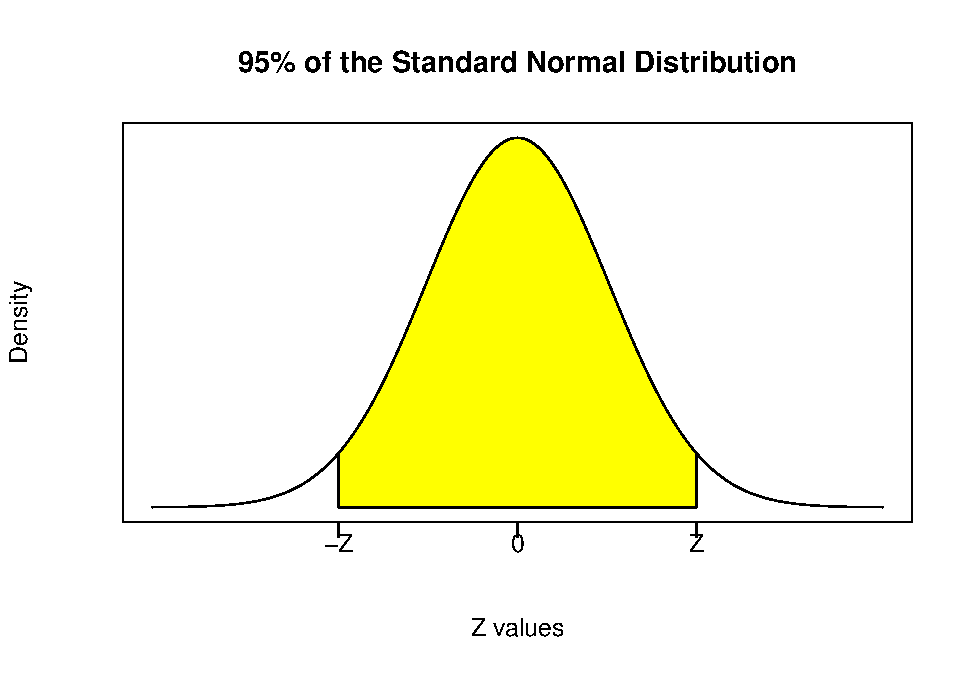
\includegraphics{MBA8350book_files/figure-latex/unnamed-chunk-70-1} \end{center}

\begin{enumerate}
\def\labelenumi{\arabic{enumi}.}
\setcounter{enumi}{1}
\tightlist
\item
  Now using the \emph{positive} critical Z value in our confidence interval equation, we have:
\end{enumerate}

\[\bar{X} \pm Z_{\frac{\alpha}{2}}\frac{\sigma}{\sqrt{n}}\]

\[10.998 \pm 1.96\frac{0.02}{\sqrt{100}}\]

Using R for the calculations:

\begin{Shaded}
\begin{Highlighting}[]
\NormalTok{Xbar }\OtherTok{=} \FloatTok{10.998}
\NormalTok{n }\OtherTok{=} \DecValTok{100}
\NormalTok{Sig }\OtherTok{=} \FloatTok{0.02}
\NormalTok{alpha }\OtherTok{=} \FloatTok{0.05}
\NormalTok{Z }\OtherTok{=} \FunctionTok{qnorm}\NormalTok{(alpha}\SpecialCharTok{/}\DecValTok{2}\NormalTok{,}\AttributeTok{lower.tail =} \ConstantTok{FALSE}\NormalTok{)}
\NormalTok{(}\AttributeTok{left =}\NormalTok{ Xbar }\SpecialCharTok{{-}}\NormalTok{ Z }\SpecialCharTok{*}\NormalTok{ Sig }\SpecialCharTok{/} \FunctionTok{sqrt}\NormalTok{(n))}
\end{Highlighting}
\end{Shaded}

\begin{verbatim}
## [1] 10.99408
\end{verbatim}

\begin{Shaded}
\begin{Highlighting}[]
\NormalTok{(}\AttributeTok{right =}\NormalTok{ Xbar }\SpecialCharTok{+}\NormalTok{ Z }\SpecialCharTok{*}\NormalTok{ Sig }\SpecialCharTok{/} \FunctionTok{sqrt}\NormalTok{(n))}
\end{Highlighting}
\end{Shaded}

\begin{verbatim}
## [1] 11.00192
\end{verbatim}

\[ 10.99408 \leq \mu \leq 11.00192 \]

Conclusion: I am 95\% confident that the mean paper length in the population is somewhere between 10.99408 and 11.00192 inches.

Note that any value within this range is equally likely!

\hypertarget{what-if-we-want-to-change-confidence}{%
\subsection{What if we want to change confidence?}\label{what-if-we-want-to-change-confidence}}

If we want to increase the confidence of our statement to 99\% or lower it 90\%, then we change \(\alpha\) and calculate a new critical Z value. Everything else stays the same.

\begin{Shaded}
\begin{Highlighting}[]
\NormalTok{alpha }\OtherTok{=} \FloatTok{0.01} \CommentTok{\# increase confidence to 99\%}
\NormalTok{Z }\OtherTok{=} \FunctionTok{qnorm}\NormalTok{(alpha}\SpecialCharTok{/}\DecValTok{2}\NormalTok{,}\AttributeTok{lower.tail =} \ConstantTok{FALSE}\NormalTok{)}
\NormalTok{(}\AttributeTok{left =}\NormalTok{ Xbar }\SpecialCharTok{{-}}\NormalTok{ Z }\SpecialCharTok{*}\NormalTok{ Sig }\SpecialCharTok{/} \FunctionTok{sqrt}\NormalTok{(n))}
\end{Highlighting}
\end{Shaded}

\begin{verbatim}
## [1] 10.99285
\end{verbatim}

\begin{Shaded}
\begin{Highlighting}[]
\NormalTok{(}\AttributeTok{right =}\NormalTok{ Xbar }\SpecialCharTok{+}\NormalTok{ Z }\SpecialCharTok{*}\NormalTok{ Sig }\SpecialCharTok{/} \FunctionTok{sqrt}\NormalTok{(n))}
\end{Highlighting}
\end{Shaded}

\begin{verbatim}
## [1] 11.00315
\end{verbatim}

\begin{Shaded}
\begin{Highlighting}[]
\NormalTok{alpha }\OtherTok{=} \FloatTok{0.10} \CommentTok{\# decrease confidence to 90\%}
\NormalTok{Z }\OtherTok{=} \FunctionTok{qnorm}\NormalTok{(alpha}\SpecialCharTok{/}\DecValTok{2}\NormalTok{,}\AttributeTok{lower.tail =} \ConstantTok{FALSE}\NormalTok{)}
\NormalTok{(}\AttributeTok{left =}\NormalTok{ Xbar }\SpecialCharTok{{-}}\NormalTok{ Z }\SpecialCharTok{*}\NormalTok{ Sig }\SpecialCharTok{/} \FunctionTok{sqrt}\NormalTok{(n))}
\end{Highlighting}
\end{Shaded}

\begin{verbatim}
## [1] 10.99471
\end{verbatim}

\begin{Shaded}
\begin{Highlighting}[]
\NormalTok{(}\AttributeTok{right =}\NormalTok{ Xbar }\SpecialCharTok{+}\NormalTok{ Z }\SpecialCharTok{*}\NormalTok{ Sig }\SpecialCharTok{/} \FunctionTok{sqrt}\NormalTok{(n))}
\end{Highlighting}
\end{Shaded}

\begin{verbatim}
## [1] 11.00129
\end{verbatim}

What happens to the size of the confidence interval when we increase our \emph{confidence}?

\hypertarget{what-to-do-when-we-do-not-know-sigma}{%
\section{\texorpdfstring{What to do when we do not know \(\sigma\)}{What to do when we do not know \textbackslash sigma}}\label{what-to-do-when-we-do-not-know-sigma}}

In most instances, if we know nothing about the population parameter \(\mu\) then we know nothing about any of the other parameters (like \(\sigma\)). In this case, we are forced to use our best guess of \(\sigma\). Since we are assuming that our sample has the same characteristics of the population, then our best guess for \(\sigma\) is the sample standard deviation \(S\).

Put plainly, we substitute the statistic (\(S\)) for the population parameter (\(\sigma\)). Because \(S\) is an estimate of \(\sigma\), this will slightly change our probability distribution. In particular, If \(\bar{X}\) is normally distributed as per the CLT, then a standardization using \(S\) instead of \(\sigma\) is said to have a t distribution with \(n-1\) degrees of freedom

\[t=\frac{\bar{X}-\mu}{(S/\sqrt{n})}\]

Note that this looks almost exactly like our Z transformation, only with \(S\) replaced for \(\sigma\). However, this statistic is said to be drawn from a distribution with \(n-1\) degrees of freedom. We mentioned degrees of freedom before, and we stated that we lose a degree of freedom when we build statistics on top of each other. In other words, we lose a degree of freedom for every statistic we use to calculate another statistic. Consider the standard deviation equation needed to calculate \(S\).

\[S = \sqrt{\frac{1}{n-1} \sum_{i=1}^n(X_i-\bar{X})^2}\]

The equation states that the sample mean \((\bar{X})\) is used to calculate the sample standard deviation. This means one statistic is used to calculate a subsequent statistic\ldots{} and that is why we lose one degree of freedom.

\hypertarget{t-distribution-versus-z-distribution}{%
\subsection{t distribution versus Z distribution\ldots{}}\label{t-distribution-versus-z-distribution}}

A t distribution and Z distribution have very much in common: they are both symmetric, both centered at a mean of 0, and both sum to one (because they are both probability distributions). The main difference is that a t-distribution has \emph{fatter tails} than a Z distribution, and the fatness of the tails depends on the degrees of freedom (which in turn depends on the sample size).

The figure below compares the standard normal (Z) distribution with several t distributions that differ in degrees of freedom. Notice that tail thickness of the t distributions are inversely related to sample size. As the the degrees of freedom get larger (i.e., the larger the sample size), the closer the t distribution gets to the Z distribution. This is because as n gets larger, \(S\) becomes a better estimate of \(\sigma\).

\begin{center}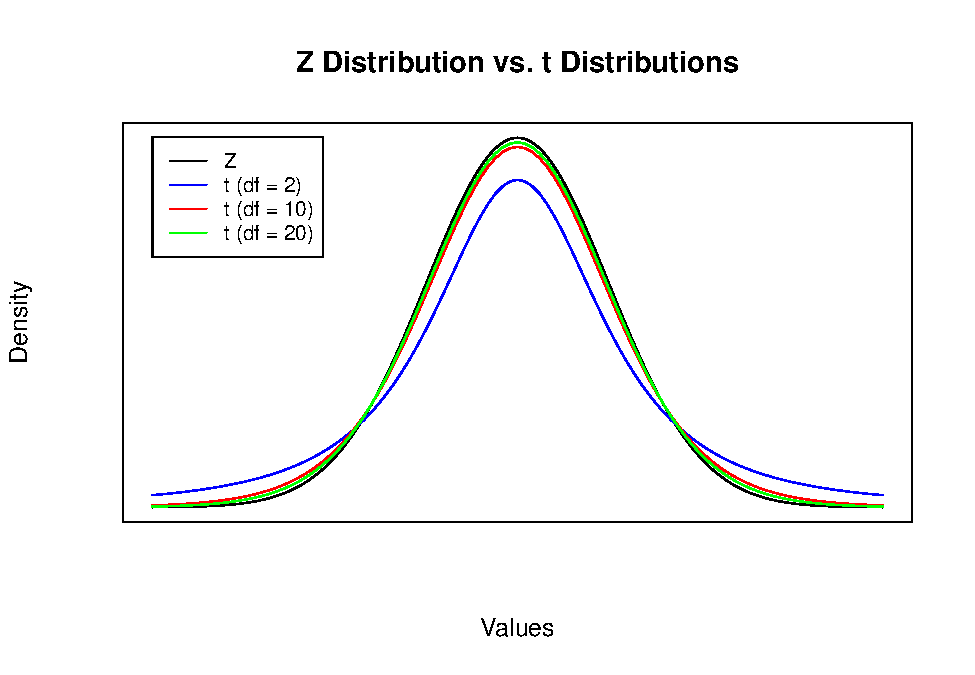
\includegraphics{MBA8350book_files/figure-latex/unnamed-chunk-73-1} \end{center}

\[\bar{X}-Z_{\frac{\alpha}{2}}\frac{\sigma}{\sqrt{n}} \leq \mu \leq \bar{X}+Z_{\frac{\alpha}{2}}\frac{\sigma}{\sqrt{n}}\]

\[\bar{X}-t_{(\frac{\alpha}{2},df=n-1)}\frac{S}{\sqrt{n}} \leq \mu \leq \bar{X}+t_{(\frac{\alpha}{2},df=n-1)}\frac{S}{\sqrt{n}}\]

In a nutshell, the only difference encountered when not knowing \(\sigma\) is that we have a slightly different probability distribution (which requires knowing the degrees of freedom and uses a different R command). The new R commands are \texttt{qt} and \texttt{pt} which requires degrees of freedom but otherwise has all of the same properties of \texttt{qnorm} and \texttt{pnorm} discussed above.

\begin{verbatim}
pt(q, df, lower.tail = TRUE)
qt(p, df, lower.tail = TRUE)
\end{verbatim}

\hypertarget{application-4}{%
\subsection{Application 4}\label{application-4}}

Suppose you manage a call center and just received a call from Quality Control asking for the \emph{average call length} at your facility. They are asking for the average call length in the population, so the best you can do is provide a confidence interval around this population parameter. You select a random sample of 50 calls from your facility and calculate a sample average of 5.8 minutes and a \textbf{sample standard deviation} of 2.815 minutes.

\[\bar{X}=5.8, \quad n=50, \quad S=2.815\]

Calculate a 95\% confidence interval around the population average call length.

\begin{Shaded}
\begin{Highlighting}[]
\NormalTok{Xbar }\OtherTok{=} \FloatTok{5.8}
\NormalTok{n }\OtherTok{=} \DecValTok{50}
\NormalTok{df }\OtherTok{=}\NormalTok{ n}\DecValTok{{-}1}
\NormalTok{S }\OtherTok{=} \FloatTok{2.815}
\NormalTok{alpha }\OtherTok{=} \FloatTok{0.05}
\NormalTok{t }\OtherTok{=} \FunctionTok{qt}\NormalTok{(alpha}\SpecialCharTok{/}\DecValTok{2}\NormalTok{,df,}\AttributeTok{lower.tail =} \ConstantTok{FALSE}\NormalTok{)}
\NormalTok{(}\AttributeTok{left =}\NormalTok{ Xbar }\SpecialCharTok{{-}}\NormalTok{ t }\SpecialCharTok{*}\NormalTok{ S }\SpecialCharTok{/} \FunctionTok{sqrt}\NormalTok{(n))}
\end{Highlighting}
\end{Shaded}

\begin{verbatim}
## [1] 4.999986
\end{verbatim}

\begin{Shaded}
\begin{Highlighting}[]
\NormalTok{(}\AttributeTok{right =}\NormalTok{ Xbar }\SpecialCharTok{+}\NormalTok{ t }\SpecialCharTok{*}\NormalTok{ S }\SpecialCharTok{/} \FunctionTok{sqrt}\NormalTok{(n))}
\end{Highlighting}
\end{Shaded}

\begin{verbatim}
## [1] 6.600014
\end{verbatim}

\emph{With 95\% confidence, the population average call length is between 5 minutes and 6.6 minutes.}

As before, if we want to change our level of confidence then we change \(\alpha\) and recalculate the t statistic. Notice that the relationship remains that a lower confidence level delivers a narrower confidence interval.

\begin{Shaded}
\begin{Highlighting}[]
\NormalTok{alpha }\OtherTok{=} \FloatTok{0.01} \CommentTok{\# increase confidence to 99\%}
\NormalTok{t }\OtherTok{=} \FunctionTok{qt}\NormalTok{(alpha}\SpecialCharTok{/}\DecValTok{2}\NormalTok{,df,}\AttributeTok{lower.tail =} \ConstantTok{FALSE}\NormalTok{)}
\NormalTok{(}\AttributeTok{left =}\NormalTok{ Xbar }\SpecialCharTok{{-}}\NormalTok{ t }\SpecialCharTok{*}\NormalTok{ S }\SpecialCharTok{/} \FunctionTok{sqrt}\NormalTok{(n))}
\end{Highlighting}
\end{Shaded}

\begin{verbatim}
## [1] 4.733108
\end{verbatim}

\begin{Shaded}
\begin{Highlighting}[]
\NormalTok{(}\AttributeTok{right =}\NormalTok{ Xbar }\SpecialCharTok{+}\NormalTok{ t }\SpecialCharTok{*}\NormalTok{ S }\SpecialCharTok{/} \FunctionTok{sqrt}\NormalTok{(n))}
\end{Highlighting}
\end{Shaded}

\begin{verbatim}
## [1] 6.866892
\end{verbatim}

\begin{Shaded}
\begin{Highlighting}[]
\NormalTok{alpha }\OtherTok{=} \FloatTok{0.10} \CommentTok{\# decrease confidence to 90\%}
\NormalTok{t }\OtherTok{=} \FunctionTok{qt}\NormalTok{(alpha}\SpecialCharTok{/}\DecValTok{2}\NormalTok{,df,}\AttributeTok{lower.tail =} \ConstantTok{FALSE}\NormalTok{)}
\NormalTok{(}\AttributeTok{left =}\NormalTok{ Xbar }\SpecialCharTok{{-}}\NormalTok{ t }\SpecialCharTok{*}\NormalTok{ S }\SpecialCharTok{/} \FunctionTok{sqrt}\NormalTok{(n))}
\end{Highlighting}
\end{Shaded}

\begin{verbatim}
## [1] 5.132563
\end{verbatim}

\begin{Shaded}
\begin{Highlighting}[]
\NormalTok{(}\AttributeTok{right =}\NormalTok{ Xbar }\SpecialCharTok{+}\NormalTok{ t }\SpecialCharTok{*}\NormalTok{ S }\SpecialCharTok{/} \FunctionTok{sqrt}\NormalTok{(n))}
\end{Highlighting}
\end{Shaded}

\begin{verbatim}
## [1] 6.467437
\end{verbatim}

\hypertarget{determining-sample-size}{%
\section{Determining Sample Size}\label{determining-sample-size}}

It was previously stated that the sample size should always be as big as possible in order to deliver the most \emph{precise} conclusions. This isn't always a satisfactory answer, because collecting observations might be possible (but costly).

How big should \(n\) be?

Selecting an appropriate sample size could be determined by many constraints

\begin{itemize}
\item
  budget, time, \ldots{} (things that cannot really be dealt with statistically)
\item
  \emph{acceptable} sampling error (we can deal with this)
\end{itemize}

Recall our confidence interval equation:

\[\bar{X}-Z_{\frac{\alpha}{2}}\frac{\sigma}{\sqrt{n}} \leq \mu \leq \bar{X}+Z_{\frac{\alpha}{2}}\frac{\sigma}{\sqrt{n}}\]

or

\[\bar{X} \pm Z_{\frac{\alpha}{2}}\frac{\sigma}{\sqrt{n}}\]

The term \(Z_{\frac{\alpha}{2}}\frac{\sigma}{\sqrt{n}}\) is one-half the width of the confidence interval. This is called the \emph{sampling error} (or \emph{margin of error}).

\[e = \pm Z_{\frac{\alpha}{2}}\frac{\sigma}{\sqrt{n}}\]

In our previous exercises, we were given a sample size \((n)\) and used our calculations to determine the width of the confidence interval \((2e)\). If we instead wanted to fix the margin of error, then we can let the above identify determine how big our sample size needs to be.

\[n = \left( \frac{Z_{\frac{\alpha}{2}}\sigma}{e}\right)^2\]

Going back to our call center example, suppose that quality control demanded a 95\% confidence interval with a 15 second (0.25 minute) margin of error. This means that the 95\% confidence interval can only be 0.5 minutes wide. How many calls need to be in the sample?

\begin{Shaded}
\begin{Highlighting}[]
\NormalTok{alpha }\OtherTok{=} \FloatTok{0.05}
\NormalTok{Z }\OtherTok{=} \FunctionTok{qnorm}\NormalTok{(alpha}\SpecialCharTok{/}\DecValTok{2}\NormalTok{,}\AttributeTok{lower.tail =} \ConstantTok{FALSE}\NormalTok{)}
\NormalTok{Xbar }\OtherTok{=} \FloatTok{5.8}
\NormalTok{Sig }\OtherTok{=} \FloatTok{2.815}
\NormalTok{e }\OtherTok{=} \FloatTok{0.25}

\NormalTok{(}\AttributeTok{n =}\NormalTok{ (Z}\SpecialCharTok{*}\NormalTok{Sig}\SpecialCharTok{/}\NormalTok{e)}\SpecialCharTok{\^{}}\DecValTok{2}\NormalTok{)}
\end{Highlighting}
\end{Shaded}

\begin{verbatim}
## [1] 487.0493
\end{verbatim}

\begin{Shaded}
\begin{Highlighting}[]
\CommentTok{\# Round up since you can\textquotesingle{}t have a fraction of an observation}
\FunctionTok{ceiling}\NormalTok{(n)}
\end{Highlighting}
\end{Shaded}

\begin{verbatim}
## [1] 488
\end{verbatim}

Our analysis indicates that if you want this particular a margin of error, then you will need to collect a sample of 488 calls.

You might have noticed that we did something a bit incorrect in the last exercise. We specified a Z distribution and called the sample standard deviation \(\sigma\). Note that only in these sort of applications that determine a sample size is this permissible. The reason is because a sample standard deviation obviously depends on the sample in question. We therefore need to assume that the standard deviation is fixed when calculating the sample size (even though this isn't the case). Once you determine a sample size, then you collect a sample, calculate the sample standard deviation, and calculate the appropriate confidence interval. The margin of error should be reasonably close to what was required.

\hypertarget{concluding-applications}{%
\section{Concluding Applications}\label{concluding-applications}}

\hypertarget{light-bulbs-last-time}{%
\subsection{Light Bulbs (Last Time)}\label{light-bulbs-last-time}}

Let's go back one last time to our light bulb example

\begin{Shaded}
\begin{Highlighting}[]
\FunctionTok{load}\NormalTok{(}\StringTok{"C:/Data/MBA8350/Lightbulb.Rdata"}\NormalTok{)}
\NormalTok{(}\AttributeTok{n =} \FunctionTok{length}\NormalTok{(Lifetime))}
\end{Highlighting}
\end{Shaded}

\begin{verbatim}
## [1] 60
\end{verbatim}

\begin{Shaded}
\begin{Highlighting}[]
\NormalTok{(}\AttributeTok{Xbar =} \FunctionTok{mean}\NormalTok{(Lifetime))}
\end{Highlighting}
\end{Shaded}

\begin{verbatim}
## [1] 907.5552
\end{verbatim}

\begin{Shaded}
\begin{Highlighting}[]
\NormalTok{(}\AttributeTok{S =} \FunctionTok{sd}\NormalTok{(Lifetime))}
\end{Highlighting}
\end{Shaded}

\begin{verbatim}
## [1] 78.96741
\end{verbatim}

We have the following information from our sample:

\[\bar{X}=907.6, \quad n = 60, \quad S = 78.967\]

Use the above information to calculate a 95\% confidence interval around the population average lifespan of the light bulbs you have left to sell. You can put this on information on the box!

\begin{Shaded}
\begin{Highlighting}[]
\NormalTok{alpha }\OtherTok{=} \FloatTok{0.05}
\NormalTok{df }\OtherTok{=}\NormalTok{ n}\DecValTok{{-}1}
\NormalTok{t }\OtherTok{=} \SpecialCharTok{{-}}\FunctionTok{qt}\NormalTok{(alpha}\SpecialCharTok{/}\DecValTok{2}\NormalTok{,df)}

\NormalTok{(}\AttributeTok{left =}\NormalTok{ Xbar }\SpecialCharTok{{-}}\NormalTok{ t }\SpecialCharTok{*}\NormalTok{ S }\SpecialCharTok{/} \FunctionTok{sqrt}\NormalTok{(n))}
\end{Highlighting}
\end{Shaded}

\begin{verbatim}
## [1] 887.1557
\end{verbatim}

\begin{Shaded}
\begin{Highlighting}[]
\NormalTok{(}\AttributeTok{right =}\NormalTok{ Xbar }\SpecialCharTok{+}\NormalTok{ t }\SpecialCharTok{*}\NormalTok{ S }\SpecialCharTok{/} \FunctionTok{sqrt}\NormalTok{(n))}
\end{Highlighting}
\end{Shaded}

\begin{verbatim}
## [1] 927.9546
\end{verbatim}

\hypertarget{returning-to-the-philadelphia-school-policy-application}{%
\subsection{Returning to the Philadelphia School Policy Application}\label{returning-to-the-philadelphia-school-policy-application}}

Let us return to the Philadelphia school policy example to provide one final discussion of a confidence interval. This application may appear redundant, but it is intended to provide an alternative approach to the confidence interval concept. It has helped students in the past, so it might do some good.

In early February 2020, the city of Philadelphia considered sending out \$100 EBT cards to every student registered in public school due to the school closings brought on by the pandemic.

\emph{How much would this policy cost?}

\hypertarget{the-frame}{%
\subsubsection*{The Frame}\label{the-frame}}
\addcontentsline{toc}{subsubsection}{The Frame}

There are 352,272 families in Philadelphia, and the city has records on how many students are registered in public schools.

However, suppose it is too costly (at this stage) to determine the total number of children registered in public schools. If we knew the average number of children registered per family, we can get an estimate of the cost of the policy.

Since it is too costly to examine the entire population (at the moment), we draw a single sample and use the sample to calculate sample statistics. Since the sample is randomly drawn from the population, the sample statistics are randomly drawn from a sampling distribution.

\begin{center}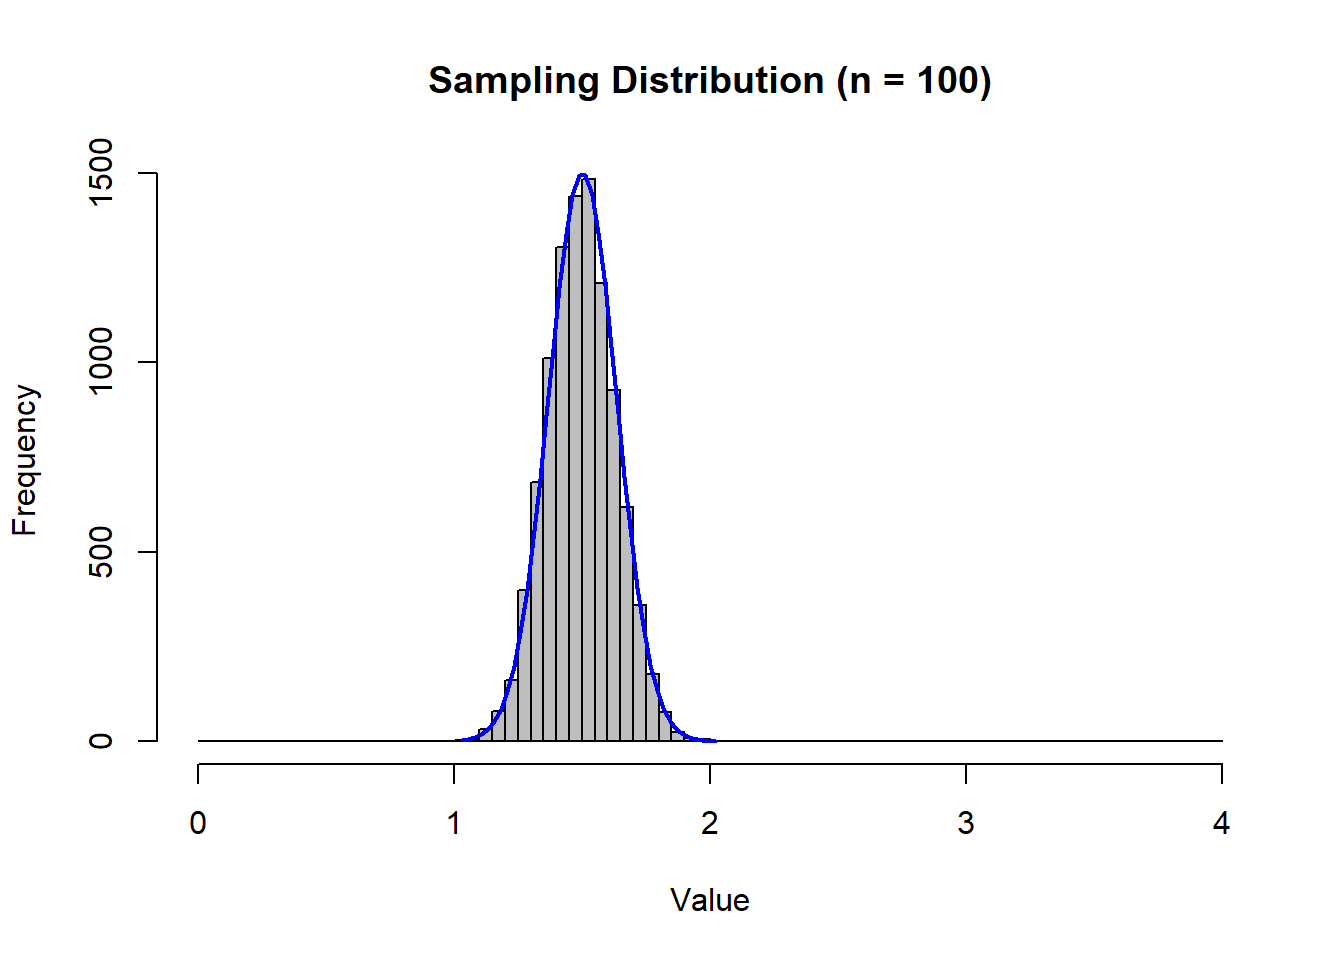
\includegraphics{MBA8350book_files/figure-latex/unnamed-chunk-80-1} \end{center}

\hypertarget{your-sample}{%
\subsubsection*{Your Sample}\label{your-sample}}
\addcontentsline{toc}{subsubsection}{Your Sample}

Once you determine a sample size \((n)\), you get \textbf{one random draw} from the appropriate sampling distribution.

\begin{itemize}
\item
  The distribution is approximately \emph{normal}
\item
  The mean is \(\mu\)
\item
  The standard deviation \(\sigma/\sqrt{n}\)
\end{itemize}

We use this information and our sample characteristics to say something about the population parameters\ldots{}

Suppose you select a sample of \(n=100\) families and calculate

\[Xbar = 1.7\]

\[S = 1.5\]

Since we have an \emph{estimate} of the population standard deviation from our sample, our sampling distribution is now a t distribution with \(n-1 = 99\) degrees of freedom.

\[ t = \frac{\bar{X}-\mu}{S/\sqrt{n}}=\frac{1.7-\mu}{1.5/\sqrt{100}}\]

\begin{center}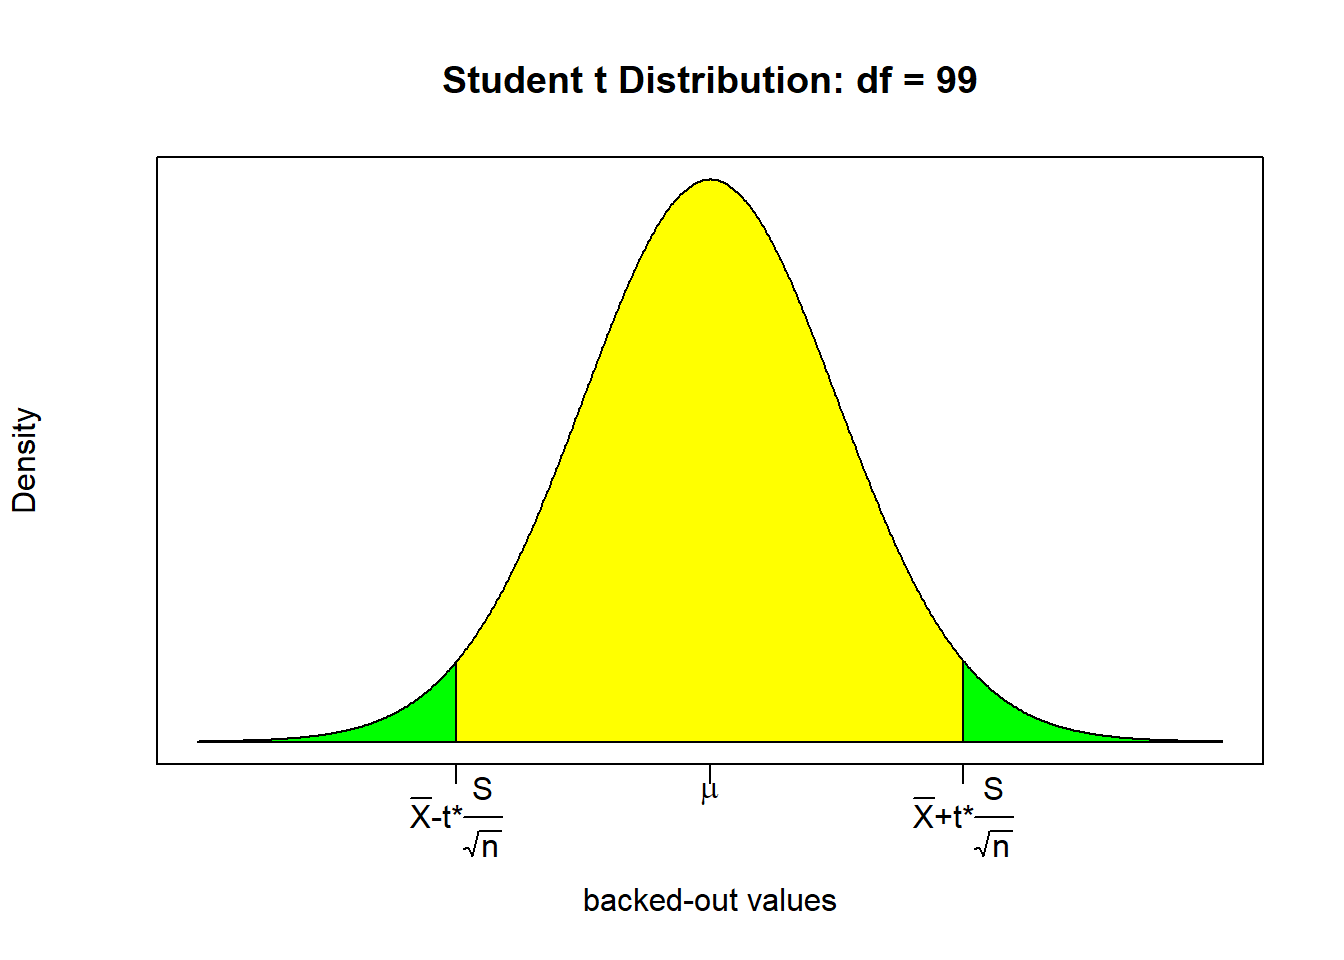
\includegraphics{MBA8350book_files/figure-latex/unnamed-chunk-81-1} \end{center}

\hypertarget{what-we-know}{%
\subsubsection*{What we know\ldots{}}\label{what-we-know}}
\addcontentsline{toc}{subsubsection}{What we know\ldots{}}

\begin{itemize}
\item
  CLT: the true population average is the central point of our sampling distribution
\item
  We can choose an \emph{arbitrary} level of confidence \((1-\alpha)\) to limit where we think our statistic from a single draw will fall.
\end{itemize}

\[Pr(-t^* \leq \frac{1.7-\mu}{1.5/\sqrt{100}} \leq t^*) = 1-\alpha\]

Suppose we want 95\% confidence \((\alpha = 0.05)\)

\begin{Shaded}
\begin{Highlighting}[]
\NormalTok{(tcrit }\OtherTok{\textless{}{-}} \FunctionTok{qt}\NormalTok{(}\FloatTok{0.05}\SpecialCharTok{/}\DecValTok{2}\NormalTok{,}\DecValTok{99}\NormalTok{))}
\end{Highlighting}
\end{Shaded}

\begin{verbatim}
## [1] -1.984217
\end{verbatim}

\begin{center}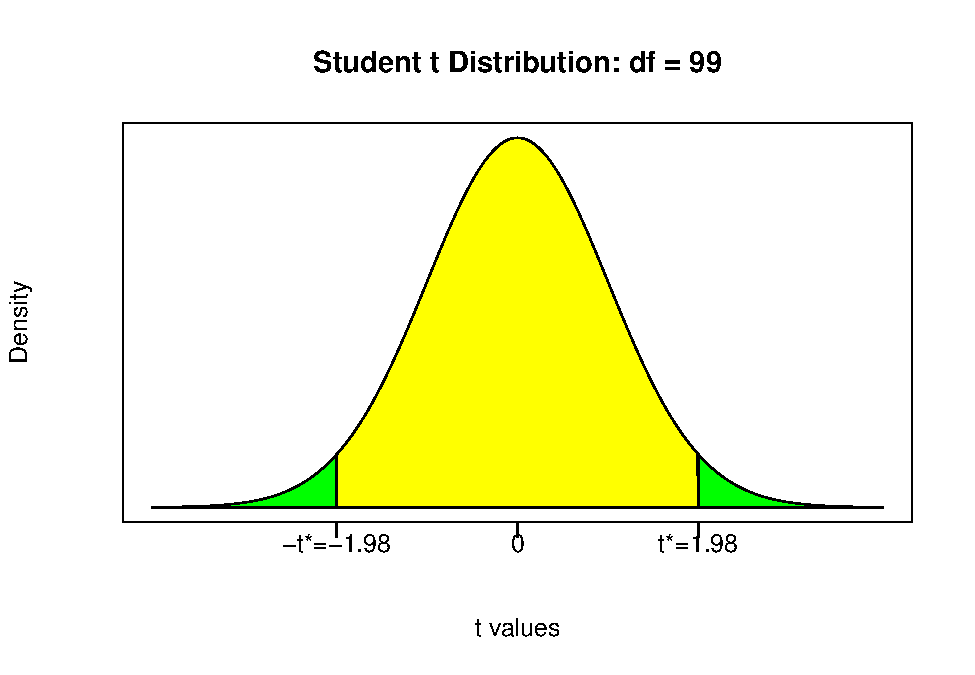
\includegraphics{MBA8350book_files/figure-latex/unnamed-chunk-83-1} \end{center}

\hypertarget{what-we-dont-know}{%
\subsubsection*{What we DON'T know\ldots{}}\label{what-we-dont-know}}
\addcontentsline{toc}{subsubsection}{What we DON'T know\ldots{}}

\begin{itemize}
\item
  We don't know the numerical value of \(\mu\)\ldots{}
\item
  We don't know where our value of \(\bar{X}\) falls in relation to \(\mu\)

  \begin{itemize}
  \item
    \(\bar{X}=\mu\)?
  \item
    \(\bar{X}>\mu\)?
  \item
    \(\bar{X}<\mu\)?
  \end{itemize}
\end{itemize}

The fact that we don't know where \(\bar{X}\) is in relation to \(\mu\) is why we end up with an \emph{interval} around where we think the population parameter resides.

\[Pr(\bar{X}-t^* \frac{S}{\sqrt{n}} \leq \mu \leq \bar{X}+t^* \frac{S}{\sqrt{n}}) = 1-\alpha\]

\[Pr(1.7-1.98 \frac{1.5}{\sqrt{100}} \leq \mu \leq 1.7+1.98 \frac{1.5}{\sqrt{100}}) = 0.95\]

\begin{center}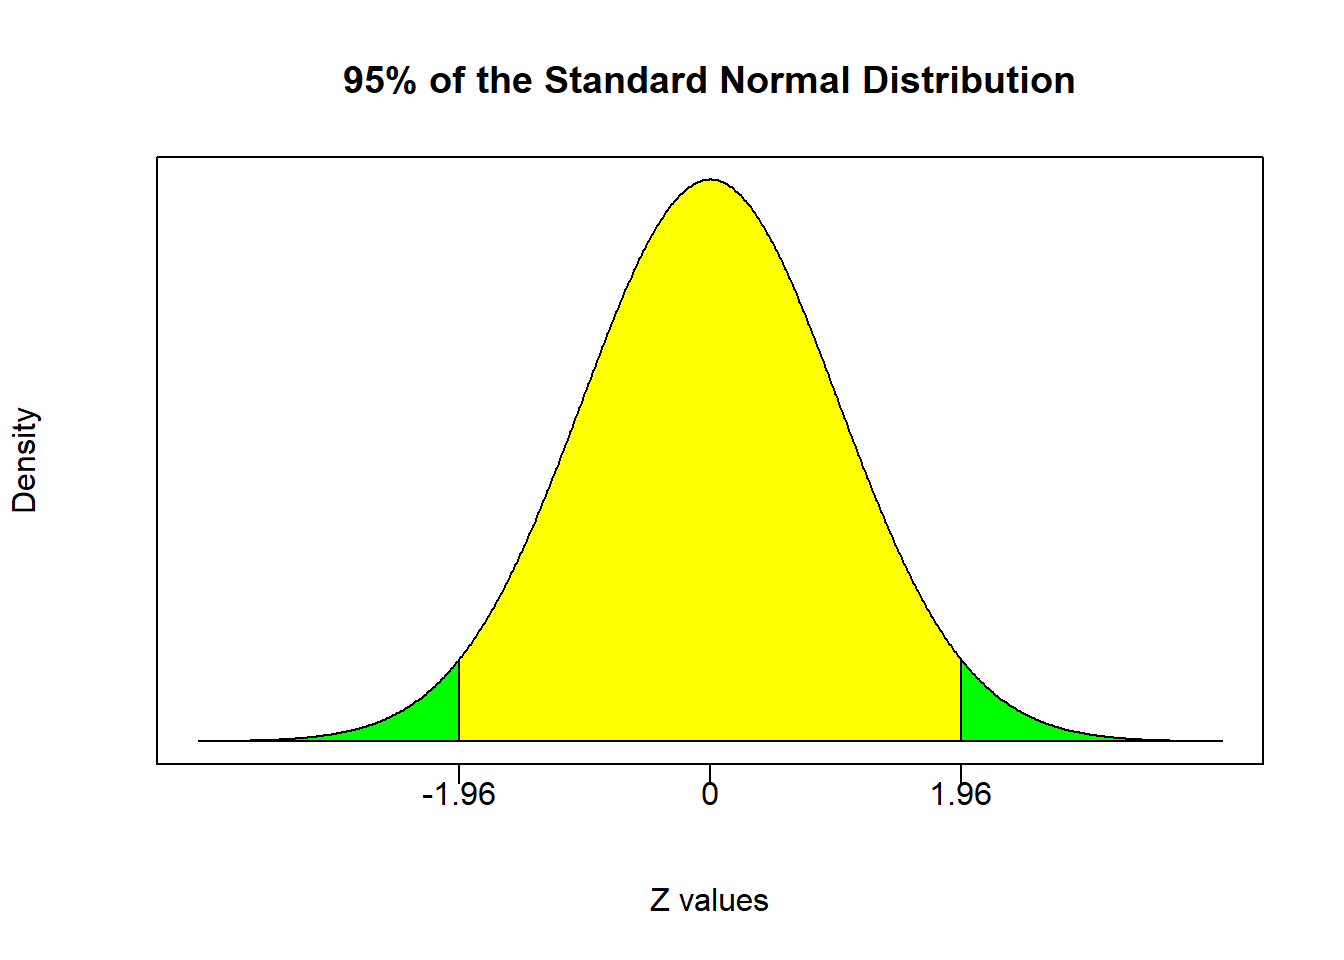
\includegraphics{MBA8350book_files/figure-latex/unnamed-chunk-84-1} \end{center}

\begin{center}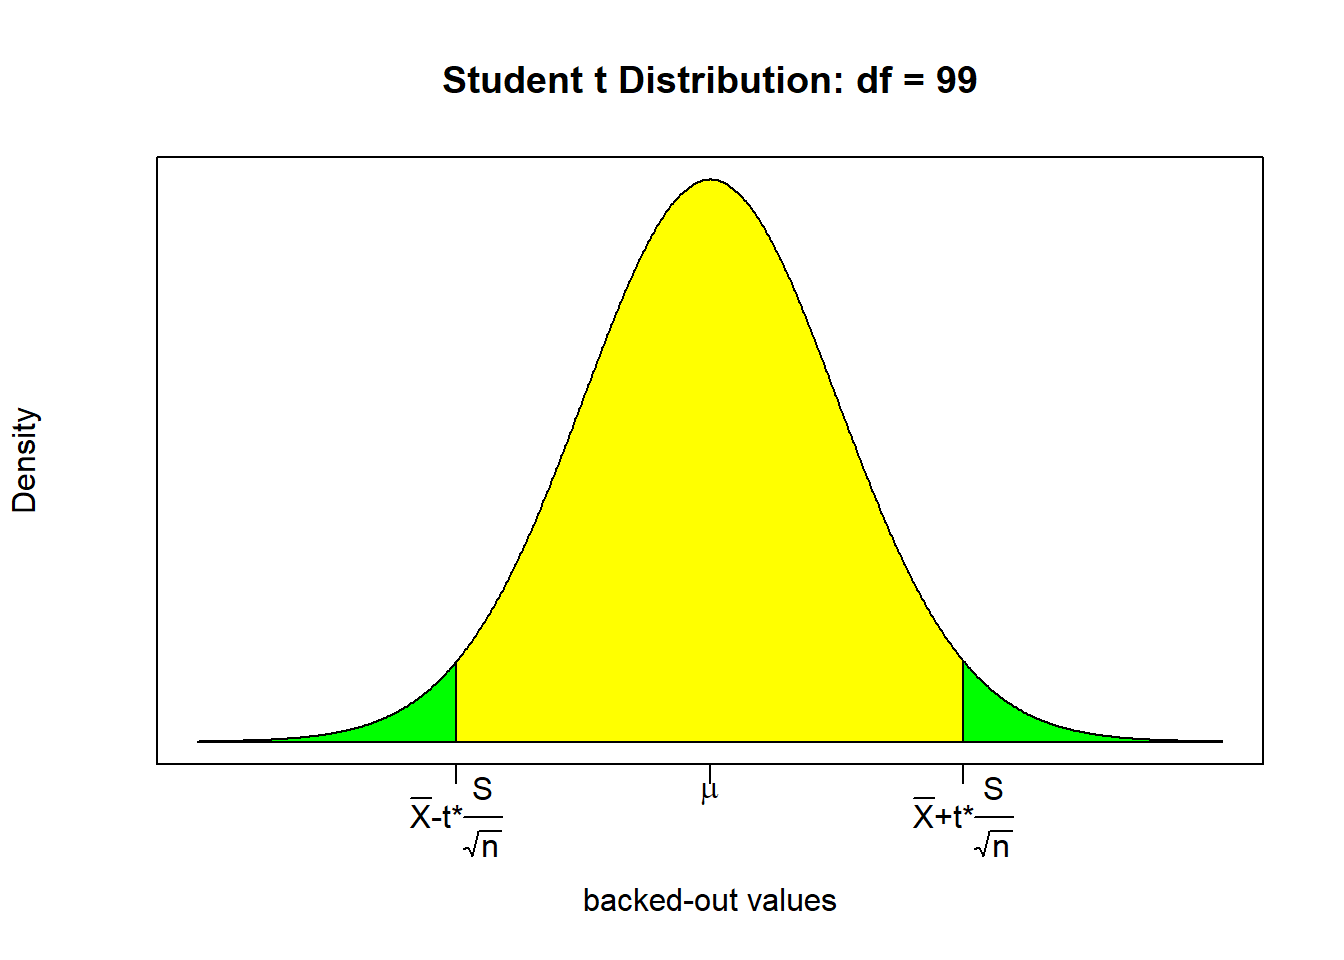
\includegraphics{MBA8350book_files/figure-latex/unnamed-chunk-85-1} \end{center}

\begin{Shaded}
\begin{Highlighting}[]
\NormalTok{Xbar }\OtherTok{=} \FloatTok{1.7}\NormalTok{; S }\OtherTok{=} \FloatTok{1.5}\NormalTok{; n }\OtherTok{=} \DecValTok{100}\NormalTok{; AL }\OtherTok{=} \FloatTok{0.05}
\NormalTok{tcrit }\OtherTok{\textless{}{-}} \SpecialCharTok{{-}}\FunctionTok{qt}\NormalTok{(AL}\SpecialCharTok{/}\DecValTok{2}\NormalTok{,n}\DecValTok{{-}1}\NormalTok{)}

\NormalTok{(LFT }\OtherTok{\textless{}{-}}\NormalTok{ Xbar }\SpecialCharTok{{-}}\NormalTok{ tcrit }\SpecialCharTok{*}\NormalTok{ S }\SpecialCharTok{/} \FunctionTok{sqrt}\NormalTok{(n))}
\end{Highlighting}
\end{Shaded}

\begin{verbatim}
## [1] 1.402367
\end{verbatim}

\begin{Shaded}
\begin{Highlighting}[]
\NormalTok{(RHT }\OtherTok{\textless{}{-}}\NormalTok{ Xbar }\SpecialCharTok{+}\NormalTok{ tcrit }\SpecialCharTok{*}\NormalTok{ S }\SpecialCharTok{/} \FunctionTok{sqrt}\NormalTok{(n))}
\end{Highlighting}
\end{Shaded}

\begin{verbatim}
## [1] 1.997633
\end{verbatim}

\[Pr(1.40 \leq \mu \leq 2.00) = 0.95\]

With 95\% confidence, the average number of children per family is between 1.4 and 2.

\emph{Total cost is between\ldots{}}

\[1.4 * \$100 * 352,272 = \$49,318,080\]

and

\[2 * \$100 * 352,272 = \$70,454,400\]

\hypertarget{HT}{%
\chapter{Hypothesis Tests}\label{HT}}

Confidence intervals determine a range where our population mean resides given the characteristics of a sample and a desired level of confidence. Recall that the population parameter can be \emph{anywhere} within the range dictated by a confidence interval.

\textbf{Hypothesis testing} is a similar inferential method, but it approaches the problem from the opposite direction.

\begin{enumerate}
\def\labelenumi{\arabic{enumi}.}
\item
  You start with an \emph{unambiguous claim} on the value of the population parameter. This claim is nonarbitrary, and dictated from either theory or a past observation.
\item
  You test to see if the sample statistics are consistent with the claim (or refute it)
\end{enumerate}

The general idea is that you begin with some \emph{nonarbitrary} statement on what value you believe (or do not believe) the population parameter to be. You then test if the characteristics of your sample suggest that it is likely or not that a population with your proposed parameter values generated a sample similar to the one you currently have.

If this seems a bit vague at the moment, it will hopefully be more concrete soon. The main thing to keep in mind is that hypothesis tests are quite simple and structured. Once you learn how to perform one hypothesis test - you can essentially perform them all. This chapter guides you through some basic steps that once mastered - you'll have a powerful tool of statistical inference under your belt.

\hypertarget{anatomy-of-a-hypothesis-test}{%
\section{Anatomy of a Hypothesis Test}\label{anatomy-of-a-hypothesis-test}}

A hypothesis test begins with a claim about the value of particular a population parameter.

This statement takes the form of a \textbf{null hypothesis}
\[H_0 : \mu = x\]

This statement gets contrasted against an \textbf{alternative hypothesis}

\[H_1 : \mu \neq x\]

The null hypothesis \((H_0)\) represents a belief of a population parameter that you would like to \emph{disprove}, while the alternative hypothesis \((H_1)\) is the opposite of the null and represents a claim you would like to show.

A hypothesis test uses the characteristics of the sample to determine if the statement about the population parameter in the null appears consistent (or inconsistent) with the characteristics of the sample. Recall that we are still under the assumption that the characteristics of the sample are similar to the \textbf{true} characteristics of the population. Therefore, if the sample characteristics are inconsistent with the statement in the null hypothesis, then you are likely to \textbf{reject the null hypothesis}. This means that the null hypothesis does not capture the \textbf{true} characteristics of the population (because the sample does). If the sample characteristics are \emph{similar} to those stated in the null hypothesis, then you do not have evidence to reject the null and you conclude to \textbf{not reject the null hypothesis}.

In other words, if you \emph{reject the null}, you have statistical evidence that \(H_1\) is correct (and the null hypothesis cannot be correct). If you \emph{do not reject the null}, you have failed to prove the alternative hypothesis. Note that failure to prove the alternative does NOT mean that you have proven the null. In other words, there IS a difference between \emph{do not reject} and \emph{accept}!

This distinction between \emph{do not reject} and \emph{accept} cannot be emphasized enough. First, if anyone concludes that they accept the null in this class - you will get marked incorrect. If you conclude to accept the null outside of this class - then people will suspect that you don't fully understand what you are talking about. Second, we can never say accept the null because it is simply too strong of a statement to make regarding a population parameter.

Suppose we believe that the population mean life span of our light bulbs is \(x\) hours. A hypothesis test will give us a specific way of testing this belief, and allows us to conclude whether or not this statement is consistent with our sample.

\[H_0:\mu=x \quad versus \quad H_1:\mu\neq x\]

We will discuss how to formally conduct a hypothesis tests in a bit. For now, lets compare these hypotheses with the confidence interval we calculated in the previous section.

\[887 \leq \mu \leq 928\]

Recall that our confidence interval states that with 95\% confidence, the population average life span of the light bulbs is \emph{somewhere} between 887 hours and 928 hours - meaning that any value within this range is equally likely. It also states that there is only a 5\% chance that the population parameter lies outside of this range.

If we were to test that the population average lifespan was 1000 hours,

\[H_0:\mu=1000 \quad versus \quad H_1:\mu\neq 1000\]

then our confidence interval would give us evidence to \textbf{reject} the null because there would be less than a 5\% chance for the null to be true. The sample characteristics and the statement in the null hypothesis are therefore inconsistent.

If we were to test that the population average lifespan was 900 hours, then we will reach a different conclusion.

\[H_0:\mu=900 \quad versus \quad H_1:\mu\neq 900\]

Since 900 is a value \emph{inside} our confidence interval, then we would not have evidence to reject the null and we therefore conclude \textbf{do not reject} the null. The reason why we never say accept is that while 900 is within the confidence interval, there are also a \emph{continuum} of other values in there. The true population mean might be 901, 900.0001, 910, etc. If you were to \emph{accept} the null, then you are explicitly stating that the population parameter is exactly 900 - we do not have enough evidence for this.

Note that while we are seeing a clear connection between hypothesis tests and confidence intervals, hypothesis tests can get more sophisticated than this. It is therefore worthwhile to consider a formal solution methodology.

\hypertarget{two-methods-for-conducting-a-hypothesis-test-when-sigma-is-known}{%
\section{\texorpdfstring{Two methods for conducting a hypothesis test (when \(\sigma\) is known)}{Two methods for conducting a hypothesis test (when \textbackslash sigma is known)}}\label{two-methods-for-conducting-a-hypothesis-test-when-sigma-is-known}}

We will consider two equivalent methods for conducting a hypothesis test. The first is called the \emph{rejection region} method and is very similar to confidence intervals. The second is the \emph{p-value} method and delivers some very useful results that we will be using for the rest of the course. We will consider these methods in turn.

\hypertarget{rejection-region-method}{%
\subsection{Rejection Region Method}\label{rejection-region-method}}

All hypothesis tests start with a statement of the null and alternative hypotheses. The null makes an explicit statement regarding the value of a population parameter \((\mu)\). Once this value of \(\mu\) is established under the null, all hypothesis tests construct a \emph{test statistic under the null}. In particular, assuming we know the population standard deviation \(\sigma\), we can construct a \emph{Z statistic under the null} using our familiar z-transformation:

\[Z = \frac{\bar{X}-\mu}{\left(\sigma / \sqrt{n} \right)}\]

Note that we already know values from the sample \((\bar{X},\;n,\;\sigma)\) and we have a \emph{hypothesized} value of \(\mu\) from the null hypothesis. We can therefore directly calculate this Z-value \emph{under the null}. This would be the value of a Z-statistic given our sample characteristics under the \emph{assumption} that our null hypothesis is correct.

The rejection region method takes this Z-statistic under the null and sees where it falls in a standard normal sampling distribution. The sampling distribution of a test statistic is first divided into two regions\ldots{}

\begin{enumerate}
\def\labelenumi{\arabic{enumi}.}
\item
  A region of rejection (a.k.a., critical region) - values of the test statistic that are unlikely to occur \textbf{if the null hypothesis is true}.
\item
  A region of nonrejection - values of the test statistic that are likely to occur if the null hypothesis is true, so they are \emph{consistent with the null hypothesis}.
\end{enumerate}

The regions of rejection and nonrejection are identified by determining \emph{critical values} of the test statistic. These are particular values of the sampling distribution that divides the entire distribution into rejection and nonrejection regions. This is why some people refer to the \emph{rejection region} approach as the \emph{critical value} approach.

Once the different regions are established, then you simply see where the calculated test statistic under the null falls. If it falls inside the rejection region, then you \textbf{reject the null} because the characteristics of the sample are \emph{too inconsistent} with the population parameter stated inside the null hypothesis. If it falls inside the nonrejection region, then you \textbf{do not reject the null} because the characteristics of the sample are such that the population parameter stated inside the null is \emph{possible} (but we can't say if it's necessarily true).

\hypertarget{the-steps-of-a-hypothesis-test-rejection-region-method}{%
\subsubsection*{The Steps of a Hypothesis Test (Rejection Region Method)}\label{the-steps-of-a-hypothesis-test-rejection-region-method}}
\addcontentsline{toc}{subsubsection}{The Steps of a Hypothesis Test (Rejection Region Method)}

\begin{enumerate}
\def\labelenumi{\arabic{enumi}.}
\item
  State the null and alternative hypotheses
\item
  Calculate a test statistic under the null
\item
  Determine the rejection and nonrejection regions of a standardized sampling distribution
\item
  Conclude (reject or do not reject)
\end{enumerate}

\hypertarget{application-1-1}{%
\subsubsection*{Application 1}\label{application-1-1}}
\addcontentsline{toc}{subsubsection}{Application 1}

Suppose a fast-food manager wants to determine whether the waiting time to place an order has changed from the previous mean of 4.5 minutes. We want to see if our sample characteristics are consistent with an average of 4.5 minutes or not. We start with a statement of the two hypotheses.

\[H_0:\mu=4.5 \quad versus \quad H_1:\mu\neq 4.5\]

The null explicitly states that \(\mu=4.5\), so we can use this value to construct a test statistic using the information from our sample. Suppose that a sample of \(n=25\) observations delivered a sample mean of \(\bar{X}=5.1\) minutes. Suppose further that we know the population standard deviation of the wait time process to be \(\sigma=1.2\). We can calculate a test statistic under the null.

\begin{Shaded}
\begin{Highlighting}[]
\NormalTok{mu }\OtherTok{=} \FloatTok{4.5}
\NormalTok{Xbar }\OtherTok{=} \FloatTok{5.1}
\NormalTok{Sig }\OtherTok{=} \FloatTok{1.2}
\NormalTok{n }\OtherTok{=} \DecValTok{25}

\NormalTok{(}\AttributeTok{Zstat =}\NormalTok{ (Xbar }\SpecialCharTok{{-}}\NormalTok{ mu)}\SpecialCharTok{/}\NormalTok{(Sig}\SpecialCharTok{/}\FunctionTok{sqrt}\NormalTok{(n)))}
\end{Highlighting}
\end{Shaded}

\begin{verbatim}
## [1] 2.5
\end{verbatim}

\[ Z = \frac{\bar{X}-\mu}{\left(\sigma / \sqrt{n} \right)} = \frac{5.1-4.5}{\left(1.2 / \sqrt{25} \right)} = 2.5\]

The next step involves taking a standard normal sampling distribution and breaking it up into regions of rejection and nonrejection. Before we do this, lets take a step back and think about what it means for a sample to be consistent or inconsistent with the null hypothesis. If you had a sample average \((\bar{X})\) that was the same value as the parameter value stated in the null hypothesis \((\mu)\) then you could state that the value of \(\mu\) in the null hypothesis is \emph{very consistent} with the characteristics of the sample. In fact, you can't be more consistent than having \(\bar{X}\) and \(\mu\) being the exact same number. Furthermore, a test statistic under the null would be equal to zero because \((\bar{X}-\mu)\) is in the numerator. This implies that a test statistic under the null equal to zero is very consistent with the null hypothesis, and you will therefore \emph{not reject} the null hypothesis. However, the farther away the test statistic under the null gets from zero, the farther away it gets from the center of the \emph{do not reject region} and the closer it gets to one of the \emph{rejection regions}.

Lets illustrate this supposing that we want to test the hypothesis at the 95\% confidence level \((\alpha=0.05)\). The central 95\% of a standard normal distribution is given by

\[Pr(-1.96 \leq Z \leq 1.96) = 0.95\]

This means that if you reached into a bowl of numbers comprising a standard normal distribution, then 95\% of the time you will draw a number between -1.96 and 1.96. The remaining numbers outside of this range will show up only 5\% of the time. These regions are the bases for confidence intervals and also the bases for the nonrejection and rejection regions.

\begin{center}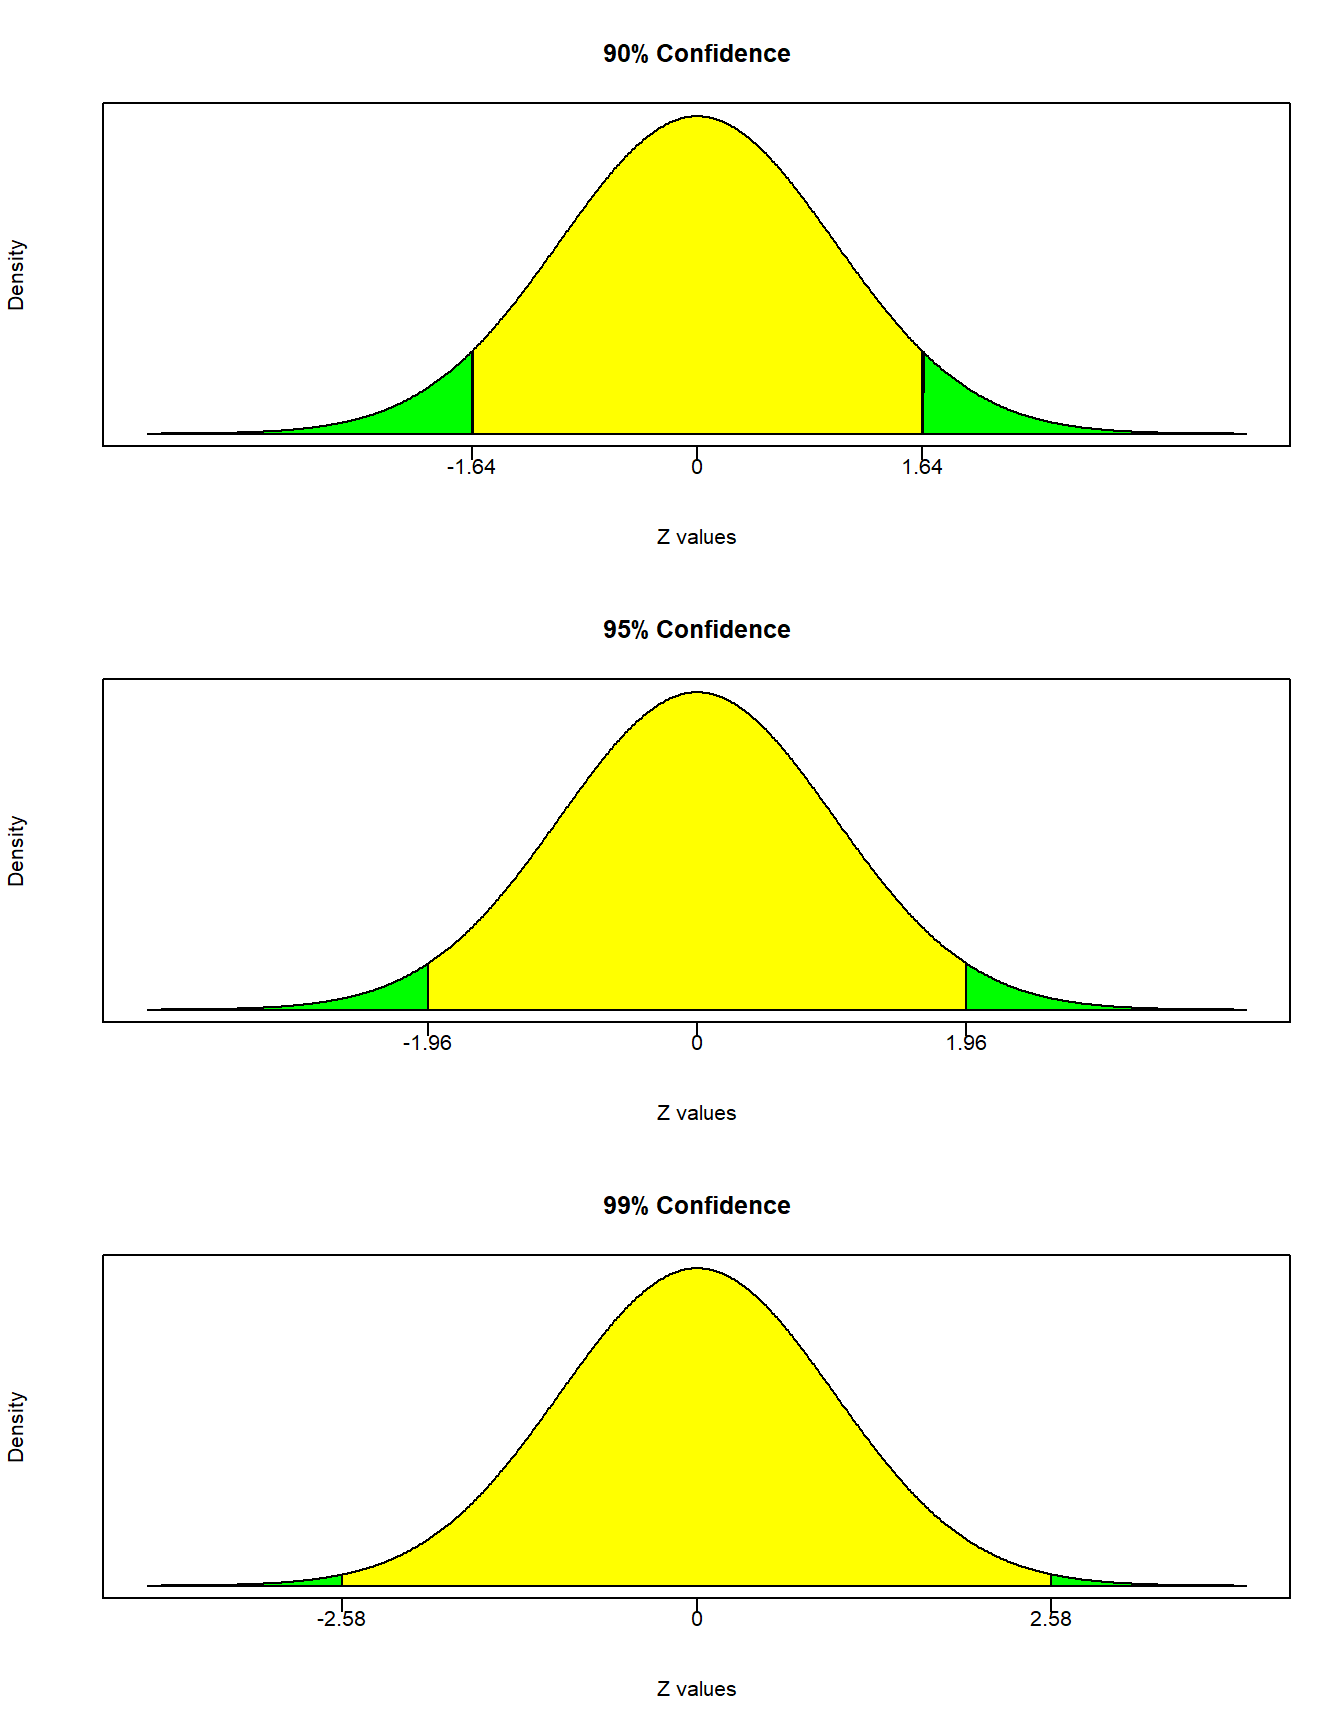
\includegraphics{MBA8350book_files/figure-latex/unnamed-chunk-89-1} \end{center}

The yellow-shaded region is centered on zero and represents the \emph{nonrejection region}. It tells you that if you calculate a test statistic under the null to be between -1.96 and 1.96, then you do not have enough evidence to reject the null. However, the green-shaded regions are the \emph{rejection regions}. It tells you that if you calculate a test statistic under the null that is greater than 1.96 or less than -1.96, then you have enough evidence to reject the null (with 95\% confidence). In other words, it is so unlikely to have the null be correct while simultaneously randomly selecting a sample with the observed sample characteristics, so we conclude that the statement in the null cannot be true. In the fast food example above, the test statistic under the null of 2.5 falls in the rejection region. This means that we can \emph{reject} the null hypothesis of \(\mu=4.5\) minutes with 95\% confidence. In other words, we are 95\% confident that the population mean is some number other than 4.5 minutes.

\textbf{Changing the level of confidence \((\alpha)\)}

The hypothesis test above was concluded under a specified 95\% confidence level \((\alpha=0.05)\). This level of confidence effectively delivered our rejection and nonrejection regions. So\ldots{} what happens when we change \(\alpha\)?

The first thing to understand is that the level of confidence does not impact the hypotheses or the test statistic under the null. The \textbf{only} thing the level of confidence impacts is the shaded regions in the sampling distribution. The figure below illustrates rejection and nonrejection regions for \(\alpha\) values of 0.10, 0.05, and 0.01. Note that as \(\alpha\) gets smaller, the size of the nonrejection region gets larger. This means that \emph{do not reject} is becoming a more likely conclusion. This should make sense because \emph{do not reject} is a wishy-washy conclusion, while \emph{reject} is definitive. Do not reject states that the null may or may not be true - it's a punt! Therefore, if you are placing more confidence on your conclusion, the more likely you are to make the wishy-washy conclusion.

The fast food example had a test statistic under the null of 2.5. This test statistic falls in the rejection region for both 90\% and 95\% levels of confidence. This suggests that if you can reject a null hypothesis with a certain level of confidence, then you can automatically reject at all lower levels of confidence. However, the do not reject region under 99\% confidence is given by
\[Pr(-2.58 \leq Z \leq 2.58)=0.99\]
and our test statistic of 2.5 falls inside it. We therefore conclude that we \emph{do NOT reject} the null with 99\% confidence. In other words, we do not have enough evidence to say that the null hypothesis is incorrect at 99\% confidence, so we conclude that it \emph{may or may not} be true (i.e., we punt).

\begin{center}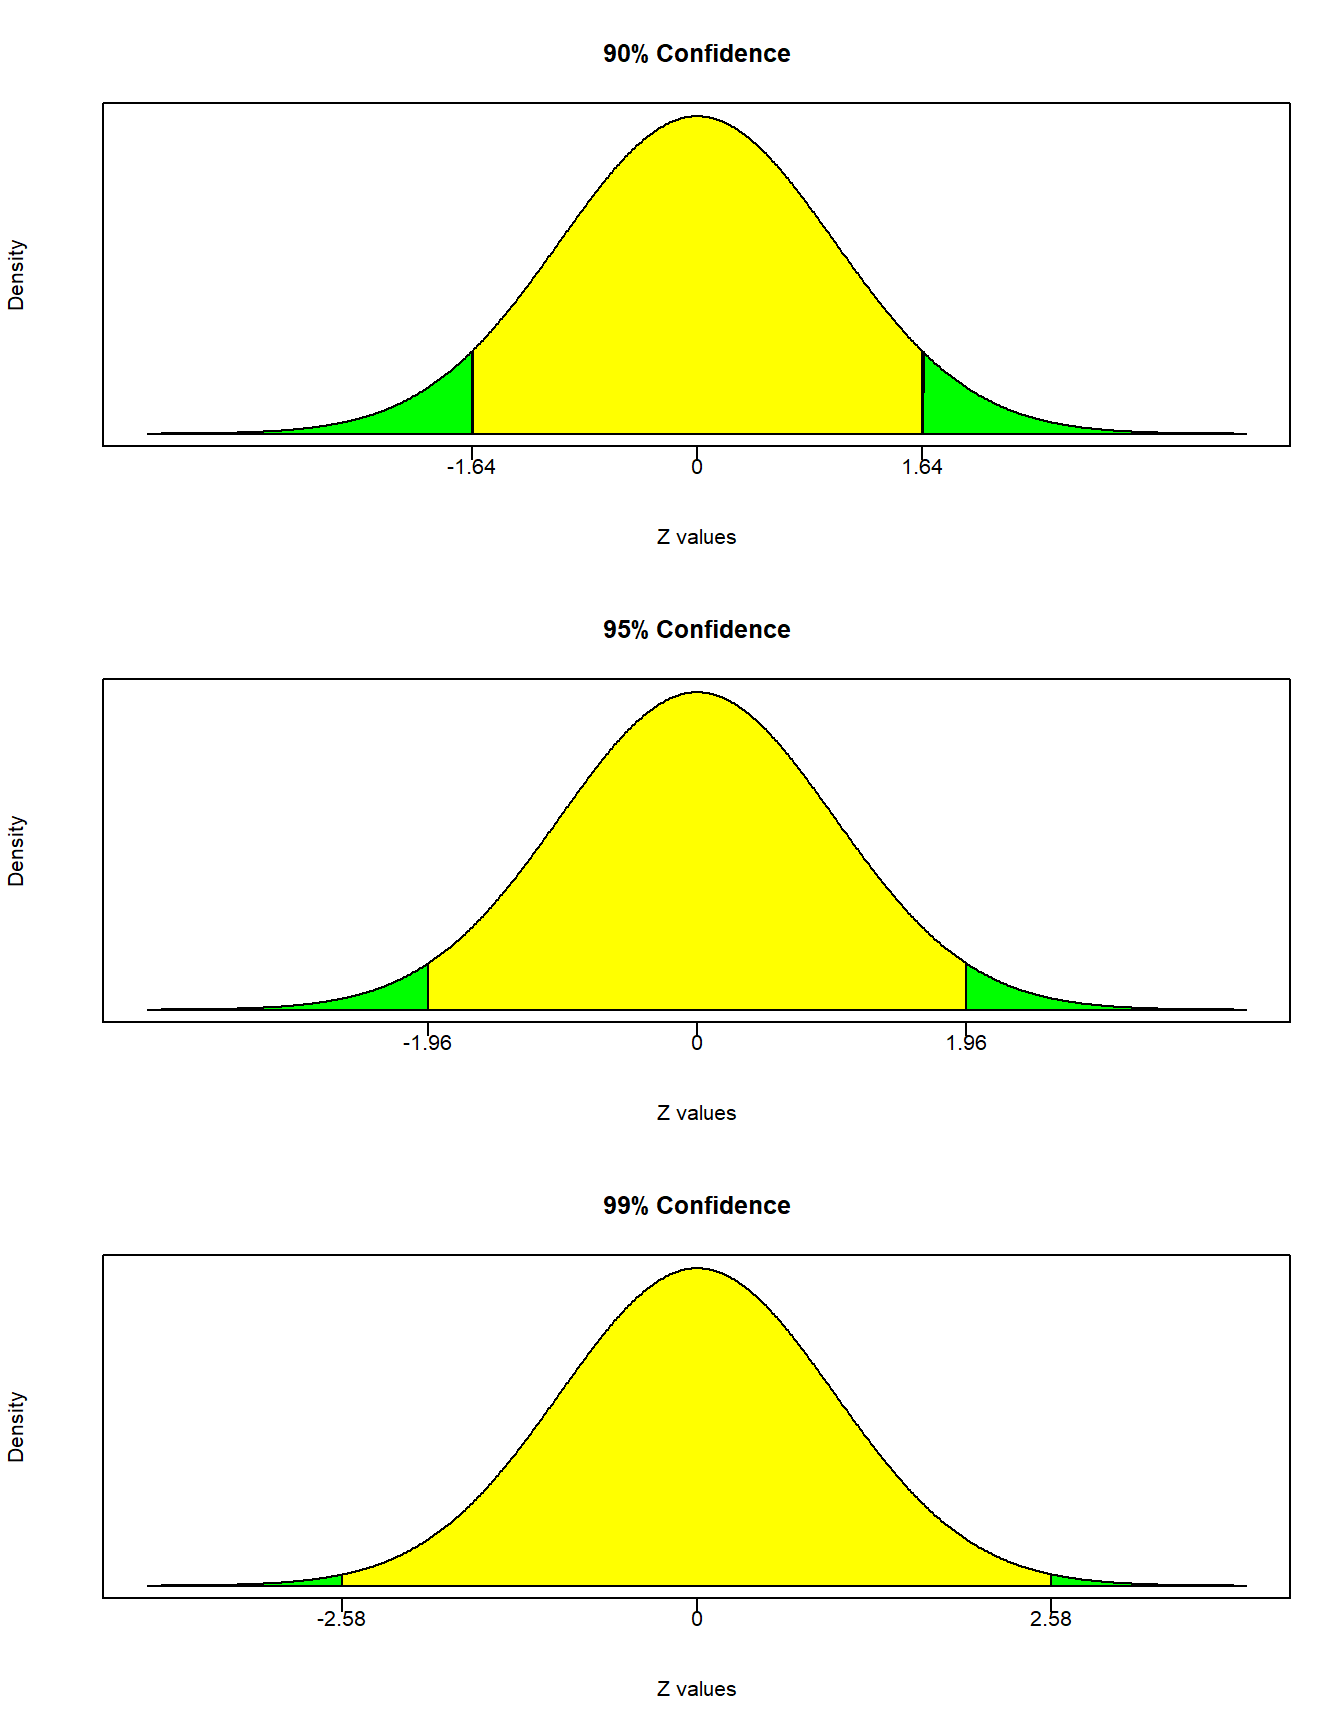
\includegraphics{MBA8350book_files/figure-latex/unnamed-chunk-90-1} \end{center}

Using the rejection region method, we were able to reject the null with 95\% confidence \((\alpha=0.05)\) but unable to reject with 99\% confidence \((\alpha=0.01)\). This begs the question as to the highest confidence level at which we can reject the null. We know it is some confidence level between 95\% and 99\%, but what is it exactly? We can use the rejection region approach multiple times by choosing various values of \(\alpha\) and narrow things down, or we can conduct the hypothesis test using the \emph{p-value} approach.

\hypertarget{p-value-approach}{%
\subsection{P-value Approach}\label{p-value-approach}}

The P-value is an extremely useful and often misunderstood number. I therefore have THREE equivalent ways of explaining it. Each one works - so just stick with the one that works for you. Before we get to those, lets talk explicitly about what we mean when we make statements based on confidence.

When using a sample statistic to draw conclusions about a population parameter, there is always the risk of reaching an incorrect conclusion. In other words, you can make an \textbf{error}.

When making a conclusion about a hypothesis test, one can either reject a null hypothesis or not. Therefore, there are two possible types of errors to be made.

\begin{enumerate}
\def\labelenumi{\arabic{enumi}.}
\item
  A \textbf{Type I error} occurs when a researcher incorrectly rejects a true hypothesis. (\emph{You rejected something that shouldn't have been rejected.})
\item
  A \textbf{Type II error} occurs when a researcher incorrectly fails to reject a false hypothesis. (\emph{You did not reject something that should have been rejected.})
\end{enumerate}

The \textbf{acceptable} probability of committing either one of these errors depends upon an arbitrary confidence level \(\alpha\). To be precise, when you reject a hypothesis with 95\% confidence, then you are implicitly stating that you are accepting a 5\% chance of being wrong. That is where \(\alpha=0.05\) (or 5\% comes from). If you decrease \(\alpha\) to 0.01 (or 1\%), then you can reject a hypothesis with 99\% confidence and implicitly accept a 1\% chance of being wrong. The kicker is that the more you decrease the probability of committing a type I error, the more you increase the chance of not rejecting a hypothesis that you should be rejecting (a type II error). For example, if you want a conclusion with 100\% confidence, then you will \emph{never} reject a hypothesis no matter how wrong it actually is.\footnote{This point touches on the idea of confidence in statistics. If you want me to make a statement with 100\% confidence, then I'll simply say \emph{anything can happen} because it is a statement that has zero chance of being wrong.}

The main take away from the previous statement is that \(\alpha\) states the \emph{acceptable} probability of committing a type one error. Recall in our fast food example that we rejected the null hypothesis with 95\% confidence (i.e., a 5\% acceptable probability of being wrong ), but we did not reject the null hypothesis with 99\% confidence (i.e., a 1\% acceptable probability of being wrong ). This means that the \emph{actual} probability of committing a type one error is somewhere in between 0.05 and 0.01 (i.e., 5\% and 1\%). This actual probability of committing a type I error is called the \textbf{p-value}.

\begin{Shaded}
\begin{Highlighting}[]
\CommentTok{\# Fast Food Example Revisited}
\NormalTok{mu }\OtherTok{=} \FloatTok{4.5}
\NormalTok{Xbar }\OtherTok{=} \FloatTok{5.1}
\NormalTok{Sig }\OtherTok{=} \FloatTok{1.2}
\NormalTok{n }\OtherTok{=} \DecValTok{25}

\NormalTok{(}\AttributeTok{Zstat =}\NormalTok{ (Xbar }\SpecialCharTok{{-}}\NormalTok{ mu)}\SpecialCharTok{/}\NormalTok{(Sig}\SpecialCharTok{/}\FunctionTok{sqrt}\NormalTok{(n)))}
\end{Highlighting}
\end{Shaded}

\begin{verbatim}
## [1] 2.5
\end{verbatim}

\begin{Shaded}
\begin{Highlighting}[]
\CommentTok{\# 95\% confidence:}
\NormalTok{alpha }\OtherTok{=} \FloatTok{0.05}
\NormalTok{(}\AttributeTok{Zcrit =} \FunctionTok{qnorm}\NormalTok{(alpha}\SpecialCharTok{/}\DecValTok{2}\NormalTok{,}\AttributeTok{lower.tail =} \ConstantTok{FALSE}\NormalTok{))}
\end{Highlighting}
\end{Shaded}

\begin{verbatim}
## [1] 1.959964
\end{verbatim}

\begin{Shaded}
\begin{Highlighting}[]
\CommentTok{\# 99\% confidence:}
\NormalTok{alpha }\OtherTok{=} \FloatTok{0.01}
\NormalTok{(}\AttributeTok{Zcrit =} \FunctionTok{qnorm}\NormalTok{(alpha}\SpecialCharTok{/}\DecValTok{2}\NormalTok{,}\AttributeTok{lower.tail =} \ConstantTok{FALSE}\NormalTok{))}
\end{Highlighting}
\end{Shaded}

\begin{verbatim}
## [1] 2.575829
\end{verbatim}

\begin{Shaded}
\begin{Highlighting}[]
\CommentTok{\# p{-}value:}
\NormalTok{(}\AttributeTok{Pval =} \FunctionTok{pnorm}\NormalTok{(Zstat,}\AttributeTok{lower.tail =} \ConstantTok{FALSE}\NormalTok{)}\SpecialCharTok{*}\DecValTok{2}\NormalTok{)}
\end{Highlighting}
\end{Shaded}

\begin{verbatim}
## [1] 0.01241933
\end{verbatim}

\begin{Shaded}
\begin{Highlighting}[]
\CommentTok{\# Actual confidence level:}
\NormalTok{((}\DecValTok{1}\SpecialCharTok{{-}}\NormalTok{Pval)}\SpecialCharTok{*}\DecValTok{100}\NormalTok{)}
\end{Highlighting}
\end{Shaded}

\begin{verbatim}
## [1] 98.75807
\end{verbatim}

The calculations regarding the fast food example were repeated and continued to include a p-value. Recall that the null hypothesis stated that the population mean was equal to 4.5, and the test statistic under the null is equal to 2.5. The critical values marking the boundaries between the do not reject region and the reject regions was \(\pm 1.96\) for \(\alpha=0.05\) and \(\pm 2.58\) for \(\alpha=0.01\). Our test statistic falls inside the rejection region for \(\alpha=0.05\) and inside the nonrejection region for \(\alpha=0.01\). Our test statistic falls \emph{right on the boundary} of a rejection and nonrejection region when \(p=0.0124\). This is the p-value of the problem. It states that you can reject the null hypothesis with \emph{at most} 98.76\% confidence and you will incur a 1.24\% chance of being wrong. As expected, it is between 5\% and 1\% and gives you a tailor-made confidence interval for the hypothesis test at hand.

\hypertarget{the-definitions-of-a-p-value}{%
\subsubsection*{The definitions of a P-value}\label{the-definitions-of-a-p-value}}
\addcontentsline{toc}{subsubsection}{The definitions of a P-value}

\begin{quote}
The p-value is the probability of getting a test statistic equal to or more extreme than the sample result, given that the null hypothesis \((H_0)\) is true.
\end{quote}

While this is the technical definition of a p-value, it is a bit vague. There are some roughly equivalent definitions that might be easier to digest.

\begin{enumerate}
\def\labelenumi{\arabic{enumi}.}
\item
  The p-value is the probability of committing a Type I error. If the p-value is greater than some arbitrarily given \(\alpha\), then you cannot reject the null.
\item
  The p-value is the probability that your null hypothesis is \emph{correct}. The HIGHEST level of confidence at which you can reject the null is therefore \(1-p\).
\end{enumerate}

\begin{center}\rule{0.5\linewidth}{0.5pt}\end{center}

\hypertarget{two-sided-vs-one-sided-test}{%
\section{Two-sided vs One-sided Test}\label{two-sided-vs-one-sided-test}}

\[H_0:\mu=4.5 \quad versus \quad H_1:\mu\neq 4.5\]

The hypothesis test considered above is known as a \textbf{two-sided} test because the null gets rejected if the mean of the sample is either significantly greater than or less than the value stated in the null hypothesis. If you notice from the illustrations above, a two-sided test has \textbf{TWO} rejection regions - one in each tail (hence the name). Note that this is also why we calculated critical values using half of the value of \(\alpha\) and doubled the calculated probability value in order to arrive at a p-value.

In the fast food example above, suppose we want to show that the service time \emph{increased}. In other words, we want statistical evidence that the wait time actually increased from a previous time of 4.5 minutes. We can provide statistical evidence by rejecting a null hypothesis that the new population average wait time is 4.5 minutes \emph{or less}. This scenario delivers us a \textbf{one-sided hypothesis test}.

\[H_0:\mu \leq 4.5 \quad versus \quad H_1:\mu> 4.5\]

As the name implies, a one-sided hypothesis test only has one rejection region. This means that the entire value of \(\alpha\) is grouped into either the right or left tail. The tail containing the rejection region depends upon the exact specification of the hypothesis test.

The hypothesis test above is called a \emph{right-tailed} test because the rejection region is in the right tail. To see this, consider several hypothetical sample averages and see if they are consistent with the null \(\mu \leq 4.5\).

\begin{itemize}
\item
  Suppose you observe \(\bar{X}=4\). Is this sample average consistent with \(\mu \leq 4.5\)?
\item
  What about \(\bar{X}=2\)?
\item
  What about \(\bar{X}=1\)?
\end{itemize}

Your answer should be yes to all of these sample averages. In fact, \emph{any} sample average less than or equal to 4.5 is consistent with \(\mu \leq 4.5\).

Next, recall the test statistic under the null:

\[ Z = \frac{\bar{X}-4.5}{\left(\sigma / \sqrt{n} \right)}\]

For any of the hypothetical values considered above (4, 2, or 1), the test statistic would be a negative number. Since we said that all of these sample averages are consistent with the null being true, then we would never reject the null in any of these instances. Therefore, the rejection region cannot be in the left tail because that is where the negative values of the distribution reside. The rejection region must therefore be in the right tail. Only when a sample average is sufficiently greater than 4.5 is when we can consider rejecting the null.

Now that we already have the null and alternative hypotheses down as well as the test statistic under the null, the next step is to determine the critical value that divides the distribution into rejection and nonrejection regions.

\begin{Shaded}
\begin{Highlighting}[]
\CommentTok{\# Fast Food Example Revisited}
\NormalTok{mu }\OtherTok{=} \FloatTok{4.5}
\NormalTok{Xbar }\OtherTok{=} \FloatTok{5.1}
\NormalTok{Sig }\OtherTok{=} \FloatTok{1.2}
\NormalTok{n }\OtherTok{=} \DecValTok{25}

\NormalTok{(}\AttributeTok{Zstat =}\NormalTok{ (Xbar }\SpecialCharTok{{-}}\NormalTok{ mu)}\SpecialCharTok{/}\NormalTok{(Sig}\SpecialCharTok{/}\FunctionTok{sqrt}\NormalTok{(n)))}
\end{Highlighting}
\end{Shaded}

\begin{verbatim}
## [1] 2.5
\end{verbatim}

\begin{Shaded}
\begin{Highlighting}[]
\CommentTok{\# 95\% confidence:}
\NormalTok{alpha }\OtherTok{=} \FloatTok{0.05}
\NormalTok{(}\AttributeTok{Zcrit =} \FunctionTok{qnorm}\NormalTok{(alpha,}\AttributeTok{lower.tail=}\ConstantTok{FALSE}\NormalTok{))}
\end{Highlighting}
\end{Shaded}

\begin{verbatim}
## [1] 1.644854
\end{verbatim}

\begin{Shaded}
\begin{Highlighting}[]
\CommentTok{\# P{-}value:}
\NormalTok{(}\AttributeTok{Pval =} \FunctionTok{pnorm}\NormalTok{(Zstat,}\AttributeTok{lower.tail=}\ConstantTok{FALSE}\NormalTok{))}
\end{Highlighting}
\end{Shaded}

\begin{verbatim}
## [1] 0.006209665
\end{verbatim}

\begin{Shaded}
\begin{Highlighting}[]
\CommentTok{\# highest Confidence Level for rejection:}
\NormalTok{((}\DecValTok{1}\SpecialCharTok{{-}}\NormalTok{Pval)}\SpecialCharTok{*}\DecValTok{100}\NormalTok{)}
\end{Highlighting}
\end{Shaded}

\begin{verbatim}
## [1] 99.37903
\end{verbatim}

\begin{center}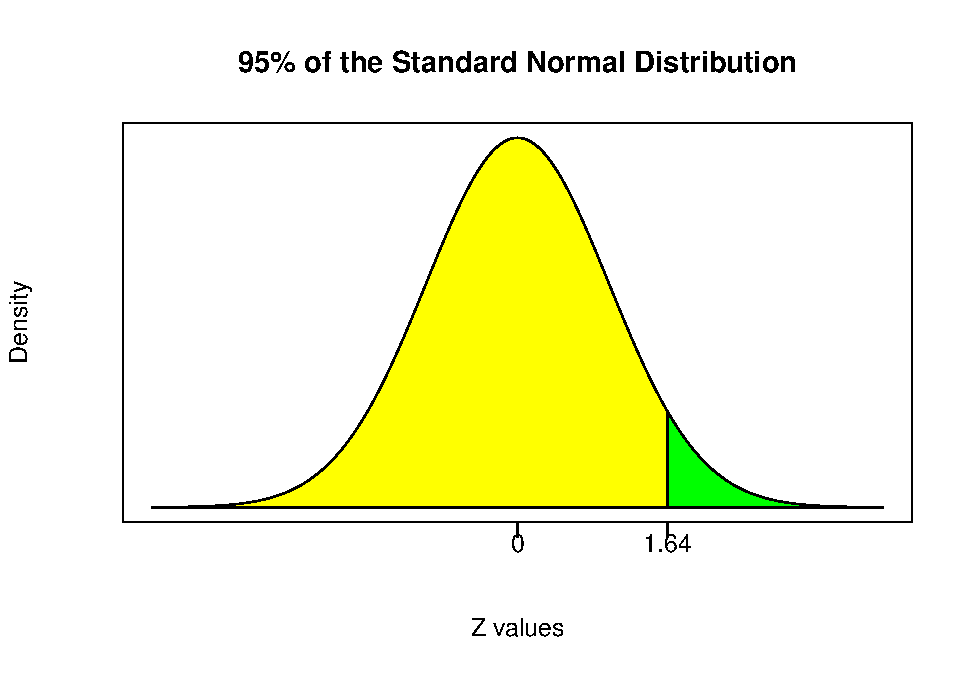
\includegraphics{MBA8350book_files/figure-latex/unnamed-chunk-93-1} \end{center}

If we conducted this hypothesis test at the 95\% confidence level (\$\alpha=0.05), you will see that the rejection region is the 5\% of the curve in the right tail. That means you reject all test statistics greater than or equal to 1.64. Since our test statistic is 2.5, we can reject with 95\% confidence. We can also conduct this hypothesis test using the p-value approach which delivers a p-value of 0.0062. This means that if we reject the null, we only incur a 0.62\% chance of being wrong. This equivalently means that we can reject the null with up to 99.38\% confidence.

\hypertarget{conducting-a-hypothesis-test-when-sigma-is-unknown}{%
\section{\texorpdfstring{Conducting a hypothesis test (when \(\sigma\) is unknown)}{Conducting a hypothesis test (when \textbackslash sigma is unknown)}}\label{conducting-a-hypothesis-test-when-sigma-is-unknown}}

When the population standard deviation \((\sigma)\) is unknown, it must be estimated. Just like with confidence intervals, When you replace \(\sigma\) with it's estimate \(S\), you change the distribution from Z to t (and need to mind the degrees of freedom).

\textbf{That's the only difference}

Let's go through some applications when \(\sigma\) is unknown. You will see that the only difference is that we use a t distribution with \(n-1\) degrees of freedom to calculate rejection / nonrejection regions and p-values.

\hypertarget{application-2-1}{%
\subsubsection*{Application 2}\label{application-2-1}}
\addcontentsline{toc}{subsubsection}{Application 2}

The Saxon Home Improvement Co.~has had a mean per sales invoice of \$120 over the last 5 years and would like to know if the mean amount per sales invoice has significantly changed. This is enough information to state our hypotheses for a two-sided test.\footnote{Note the language - \emph{significantly changed} means that the value could have either gone up or down. This is why it is a two-sided test.}

\[H_0:\mu=120 \quad versus \quad H_0:\mu \neq 120\]

You collected a sample of 12 observations, and concluded that the sample mean was \$112.85 and the sample standard deviation was \$20.80.

\[\bar{X}=112.85, \quad n=12, \quad S=20.80\]

This information allows us to calculate a t-test statistic under the null. The only difference is that we now have a sample standard deviation \((S)\) were we once had a population standard deviation \((\sigma)\).

\begin{Shaded}
\begin{Highlighting}[]
\NormalTok{Xbar }\OtherTok{=} \FloatTok{112.85}
\NormalTok{n }\OtherTok{=} \DecValTok{12}
\NormalTok{S }\OtherTok{=} \FloatTok{20.80}
\NormalTok{mu }\OtherTok{=} \DecValTok{120}

\NormalTok{(}\AttributeTok{t =}\NormalTok{ (Xbar }\SpecialCharTok{{-}}\NormalTok{ mu) }\SpecialCharTok{/}\NormalTok{ (S}\SpecialCharTok{/}\FunctionTok{sqrt}\NormalTok{(n)))}
\end{Highlighting}
\end{Shaded}

\begin{verbatim}
## [1] -1.190785
\end{verbatim}

\[ t = \frac{\bar{X}-\mu}{\left(S / \sqrt{n} \right)}=\frac{112.85-120}{\left(20.80 / \sqrt{12} \right)}=-1.19\]

Now that we have our test statistic, we need to determine if it falls into our nonrejection or rejection regions. The important thing to realize is that these regions are now part of a t distribution with 11 \((n-1)\) degrees of freedom. If we consider 95\% confidence\ldots{}

\begin{Shaded}
\begin{Highlighting}[]
\NormalTok{alpha }\OtherTok{=} \FloatTok{0.05}
\NormalTok{(}\AttributeTok{tcrit =} \FunctionTok{qt}\NormalTok{(alpha}\SpecialCharTok{/}\DecValTok{2}\NormalTok{,n}\DecValTok{{-}1}\NormalTok{,}\AttributeTok{lower.tail=}\ConstantTok{FALSE}\NormalTok{))}
\end{Highlighting}
\end{Shaded}

\begin{verbatim}
## [1] 2.200985
\end{verbatim}

The calculations suggest that the nonrejection region is between \(\pm 2.2\). Since our test statistic falls within this region, we do not reject the null. This implies that we do not have evidence that the population average sales invoice has significantly changed from \$120 with 95\% confidence. The conclusion is therefore \emph{do not reject}.

We could also calculate a p-value for the test:

\begin{Shaded}
\begin{Highlighting}[]
\NormalTok{(}\AttributeTok{Pval =} \FunctionTok{pt}\NormalTok{(t,n}\DecValTok{{-}1}\NormalTok{)}\SpecialCharTok{*}\DecValTok{2}\NormalTok{)}
\end{Highlighting}
\end{Shaded}

\begin{verbatim}
## [1] 0.2588003
\end{verbatim}

\begin{Shaded}
\begin{Highlighting}[]
\CommentTok{\# Highest confidence interval for rejection:}
\NormalTok{((}\DecValTok{1}\SpecialCharTok{{-}}\NormalTok{Pval)}\SpecialCharTok{*}\DecValTok{100}\NormalTok{)}
\end{Highlighting}
\end{Shaded}

\begin{verbatim}
## [1] 74.11997
\end{verbatim}

Notice here that the p-value states that if we were to reject the null, then we would incur a 25.88\% chance of being wrong. This means that we could only reject the null with 74.12\% confidence.

Note that the calculations uses a new R command: \texttt{pt(q,df)}. This command calculates the probability under a t distribution the same way the \texttt{pnorm(q)} command calculates the probability under a standard normal distribution. In addition, I again encourage you to always visualize the distribution and explicitly draw the rejection and nonrejection regions. This is extremely helpful when first getting started. Below you will also see a note I wrote for a previous class reinforcing how R likes to calculate probabilities. It is for reference if needed.

\hypertarget{appendix-a-note-on-calculating-p-values}{%
\section{Appendix: A note on calculating P-values}\label{appendix-a-note-on-calculating-p-values}}

\hypertarget{the-problem}{%
\subsection{The Problem}\label{the-problem}}

Suppose you were performing a right-tailed hypothesis test (using a t distribution) and you arrived at a test statistic under the null of \(1.57\). This means that the rejection region is in the right tail, and if you wished to calculate the p-value, then it would be the area of the curve to the right of \(1.57\).

If you have a sample of \(n = 50\), then you would use a t-distribution with \(49\) or \((n-1)\) degrees of freedom.

An illustration is below:

\begin{center}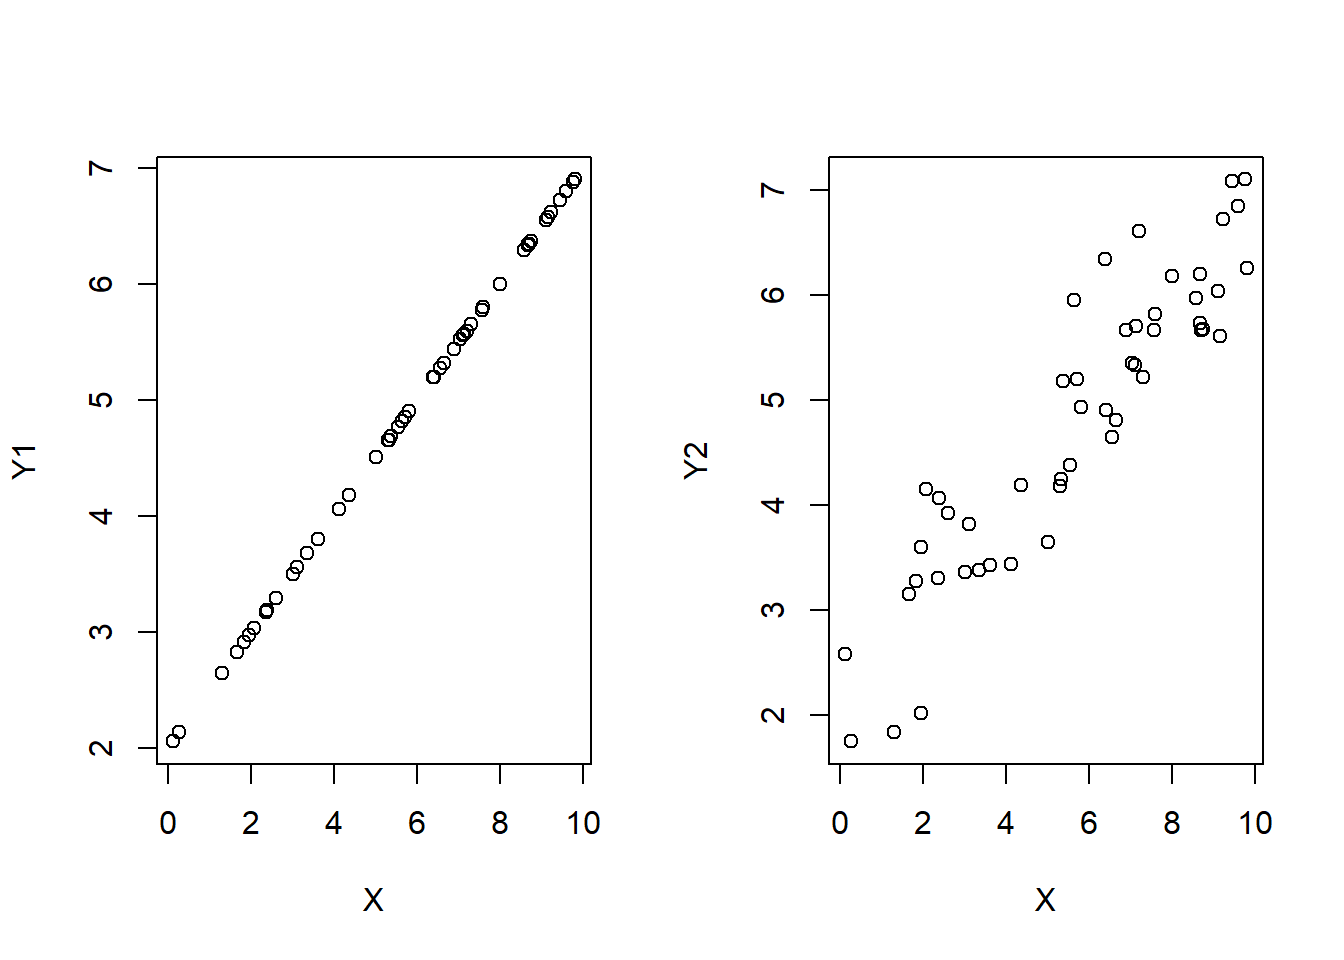
\includegraphics{MBA8350book_files/figure-latex/unnamed-chunk-98-1} \end{center}

\hypertarget{how-to-calculate-p-values}{%
\subsection{How to calculate p-values}\label{how-to-calculate-p-values}}

In case you haven't noticed by now, R has a default way of calculating probability areas\ldots{}

\emph{IT ALWAYS CALCULATES AREAS FROM THE LEFT!}

In other words, the default is to give you the area to the left of a number\ldots{}

\begin{Shaded}
\begin{Highlighting}[]
\NormalTok{(}\AttributeTok{Pval =} \FunctionTok{pt}\NormalTok{(}\FloatTok{1.57}\NormalTok{,}\DecValTok{49}\NormalTok{))}
\end{Highlighting}
\end{Shaded}

\begin{verbatim}
## [1] 0.9385746
\end{verbatim}

Don't be annoyed about this, because all software does this (including Excel).

We can use this default to calculate the p-value (i.e.~the area to the right of 1.57) in THREE different ways by relying on two properties of our probability distributions.

\textbf{Property 1:} The distribution is centered at zero and symmetric.

This means that the area to the right of 1.57 is the same as the area to the left of -1.57. So we can use the pt function with the default setting to this effect:

\begin{Shaded}
\begin{Highlighting}[]
\NormalTok{(}\AttributeTok{Pval =} \FunctionTok{pt}\NormalTok{(}\SpecialCharTok{{-}}\FloatTok{1.57}\NormalTok{,}\DecValTok{49}\NormalTok{))}
\end{Highlighting}
\end{Shaded}

\begin{verbatim}
## [1] 0.06142544
\end{verbatim}

\textbf{Property 2:} The distribution always adds up to one.

This means that you have a 100\% chance of pulling a number between negative and positive infinity. So if you use 1.57 and the default setting which gives you the area to the left, then subtract that number from 1 to get the area to the right:

\begin{Shaded}
\begin{Highlighting}[]
\NormalTok{(}\AttributeTok{Pval =} \DecValTok{1}\SpecialCharTok{{-}}\FunctionTok{pt}\NormalTok{(}\FloatTok{1.57}\NormalTok{,}\DecValTok{49}\NormalTok{))}
\end{Highlighting}
\end{Shaded}

\begin{verbatim}
## [1] 0.06142544
\end{verbatim}

\textbf{Final Option: Undo the default setting\ldots{}}

The full command for calculating a p-value from a t-distribution (for our purposes) is as follows:

pt(q, df, lower.tail = TRUE)

Note that \(q\) is the \emph{quantity}, and \(df\) is the \emph{degrees of freedom}. All other entries (if not specified) go to their default values. This is where \(lower.tail\) comes in. It is set to \emph{TRUE} by default, meaning that whatever number you input for q, you will get the area to the left. If you change this entry to \emph{FALSE}, then the default is switched off and you will calculate the area to the right.

\begin{Shaded}
\begin{Highlighting}[]
\NormalTok{(}\AttributeTok{Pval =} \FunctionTok{pt}\NormalTok{(}\FloatTok{1.57}\NormalTok{,}\DecValTok{49}\NormalTok{,}\AttributeTok{lower.tail =} \ConstantTok{FALSE}\NormalTok{))}
\end{Highlighting}
\end{Shaded}

\begin{verbatim}
## [1] 0.06142544
\end{verbatim}

Notice that all three ways of calculating a p-value give you the exact same result. Therefore, you do not need to master all three - just pick whichever method works best for you.

\hypertarget{SLR}{%
\chapter{Simple Linear Regression}\label{SLR}}

Suppose you have two homes that are the same in \emph{every way} except for size. Our intuition would suggest that bigger homes cost more (\emph{all else equal}) so we would expect that there is a positive relationship between house size and house price.

Saying \emph{bigger homes cost more} is a \textbf{qualitative} statement because all we are saying is that the relationship between house size and house price is positive. What if we want to make a \textbf{quantitative} statement? In other words, while we are fairly confident that the actual house price (say, in dollars) will increase for every unit increase in house size (say, an additional square foot) - we want to know exactly what this \emph{average-price-per-square-foot} is.

A \textbf{Regression} can measure the relationship between the mean value of one variable and corresponding values of other variables. In other words, it is a statistical technique used to explain average movements of one (dependent) variable, as a function of movements in a set of other (independent) variables.

This chapter will discuss the estimation, interpretation, and statistical inference of a \emph{simple} linear regression model, which means that we will attempt to explain the movements in a dependent variable by considering \textbf{one} independent variable. This is the simplest regression model we can consider in order to understand what is going on under the hood of a regression. The next chapter will extend this analysis to \emph{multiple} regression models where the only real difference is that the number of independent variables are greater than one.

\hypertarget{a-simple-linear-regression-model}{%
\section{A Simple Linear Regression Model}\label{a-simple-linear-regression-model}}

A Linear Regression model is a line equation.

The simplest example of a line equation is:

\[Y_i=\beta_0+\beta_1X_i\]

The \emph{betas}, \(\beta_0\) and \(\beta_1\) are called line coefficients.

\begin{itemize}
\item
  \(\beta_0\) is the \emph{constant} or \emph{intercept term}
\item
  \(\beta_1\) is the \emph{slope} term - it determines the change in Y given a change in X
\end{itemize}

\[\beta_1=\frac{Rise}{Run}=\frac{\Delta Y_i}{\Delta X_i}\]

\hypertarget{what-does-a-regression-model-imply}{%
\subsection{What does a regression model imply?}\label{what-does-a-regression-model-imply}}

\[Y_i=\beta_0+\beta_1X_i\]

When we write down a model like this, we are imposing a huge amount of assumptions on how we believe the world works.

First, there is the \textbf{Direction of causality}. A regression implicitly assumes that changes in the independent variable (X) \emph{causes} changes in the dependent variable (Y). This is the ONLY direction of causality we can handle, otherwise our analysis would be confounded (\textbf{what causes what}) and not useful.

Second, The equation assumes that information on the independent variable (X) is all the information you need to explain the dependent variable (Y). In other words, if we were to look at pairs of observations of X and Y on a plot, then the above equation assumes that all observations (data points) line up exactly on the regression line.

This would be great if the observations look like the figure on the left, but not if they look like the figure on the right.

\begin{center}\includegraphics{MBA8350book_files/figure-latex/unnamed-chunk-104-1} \end{center}

It would be extremely rare for the linear model (as detailed above) to account for all there is to know about the dependent variable Y\ldots{}

\begin{enumerate}
\def\labelenumi{\arabic{enumi}.}
\item
  There might be other independent variables that explain different parts of the dependent variable (i.e., multiple dimensions). \emph{(more on this next chapter)}
\item
  There might be measurement error in the recording of the variables.
\item
  There might be an incorrect functional form - meaning that the relationship between the dependent and independent variable might be more sophisticated than a straight line. \emph{(more on this next chapter)}
\item
  There might be purely random and therefore totally unpredictable variation in the dependent variable.
\end{enumerate}

This last item can be easily dealt with!

Adding a stochastic error term (\(\varepsilon_i\)) to the model will effectively take care of all sources of variation in the dependent variable (Y) that is not explicitly captured by information contained in the independent variable (X).

\hypertarget{the-real-simple-linear-regression-model}{%
\subsection{\texorpdfstring{The \emph{REAL} Simple Linear Regression Model}{The REAL Simple Linear Regression Model}}\label{the-real-simple-linear-regression-model}}

\[Y_i=\beta_0+\beta_1X_i+\varepsilon_i\]

The Linear Regression Model now explicitly states that the explanation of the dependent variable \((Y_i)\) can be broken down into two components:

\begin{itemize}
\item
  A \textbf{Deterministic} Component: \(\beta_0+\beta_1X_i\)
\item
  A \textbf{Random / Stochastic / Explainable} Component: \(\varepsilon_i\)
\end{itemize}

Lets address these two components in turn.

\hypertarget{the-deterministic-component}{%
\subsubsection*{The Deterministic Component}\label{the-deterministic-component}}
\addcontentsline{toc}{subsubsection}{The Deterministic Component}

\[\hat{Y}_i=\beta_0+\beta_1X_i\]

The deterministic component delivers the expected (or \emph{average}) value of the dependent variable (Y) given a values for the coefficients (\(\beta_0\) and \(\beta_1\)) and a value of the dependent variable (X).

Since X is given, it is considered \emph{deterministic} (i.e., non-stochastic)

In other words, the deterministic component determines the mean value of Y associated with a particular value of X. This should make sense, because the average value of Y is the best guess.

Technically speaking, the deterministic component delivers the \emph{expected value of Y conditional on a value of X} (i.e., a conditional expectation).

\[\hat{Y}_i=\beta_0+\beta_1X_i=E[Y_i|X_i]\]

\hypertarget{the-unexpected-garbage-can-component}{%
\subsubsection*{\texorpdfstring{The Unexpected (\emph{Garbage Can}) Component}{The Unexpected (Garbage Can) Component}}\label{the-unexpected-garbage-can-component}}
\addcontentsline{toc}{subsubsection}{The Unexpected (\emph{Garbage Can}) Component}

\[\varepsilon_i=Y_i-\hat{Y}_i\]

Once we obtain the coefficients, we can compare the observed values of \(Y_i\) with the expected value of \(Y_i\) conditional on the values of \(X_i\).

The difference between the true value \((Y_i)\) and the expected value \((\hat{Y}_i)\) is by definition\ldots{} \emph{unexpected!}

This unexpected discrepancy is your \textbf{prediction error} - and everything your deterministic component cannot explain is deemed \emph{random} and \emph{unexplainable}.

If a portion of the dependent variable is considered random and unexplainable - then it gets thrown away into the \emph{garbage can} (\(\varepsilon_i\)).

This is a subtle but crucial part of regression modeling\ldots{}

\begin{itemize}
\item
  Your choice of the independent variable(s) dictate what you believe to be important in explaining the dependent variable.
\item
  The unimportant (or random) changes in the dependent variable that your independent variables cannot explain end up in the garbage can \emph{by design}.
\item
  Therefore, \textbf{the researcher} essentially chooses what is important, and what gets thrown away into the garbage can.
\end{itemize}

\textbf{YOU are the researcher}, so \textbf{YOU} determine what goes into the garbage can!

\hypertarget{application-predicting-house-price-based-on-house-size}{%
\section{Application: Predicting House Price Based on House Size}\label{application-predicting-house-price-based-on-house-size}}

Let's consider an application where we attempt to explain the price of a house (in thousand US\$) by the size of a house (in square feet). We start by establishing the theory and relating it to our statistical terminology.

\textbf{The Population Regression Function:}

\[Price_i = \beta_0 + \beta_i Size_i + \varepsilon_i\]

\begin{itemize}
\item
  \(Price_i\) is the dependent variable (\(Y_i\))
\item
  \(Size_i\) is the independent variable (\(X_i\))
\item
  The equation above is the true (but unknown), population regression function.
\item
  The coefficients (\(\beta_0\) and \(\beta_1\)) are the population regression coefficients!

  \begin{itemize}
  \item
    They are the coefficients you would obtain if you had \emph{every} possible observation (i.e., the population)
  \item
    This ain't gonna happen\ldots{}
  \end{itemize}
\item
  We need to obtain the estimated, sample regression coefficients. To do this, we need to collect a sample of observations.
\end{itemize}

\textbf{The Sample}

In order to obtain \emph{sample estimates} of our regression model above, we must obtain a sample of observations. We collect a (random) sample of size \(n\). This is where the subscript i comes in - indicating that in general, each individual observation can be identified as \(i=1,...,n\). The sample estimates are based on the sample.

Hypothetically, we can obtain different estimated coefficients for every different sample\ldots{} but we will address that later.

To facilitate this application, we will use a data set internal to R, called \emph{hprice1}.

\begin{Shaded}
\begin{Highlighting}[]
\FunctionTok{data}\NormalTok{(hprice1,}\AttributeTok{package=}\StringTok{\textquotesingle{}wooldridge\textquotesingle{}}\NormalTok{)}
\FunctionTok{ls}\NormalTok{(hprice1)}
\end{Highlighting}
\end{Shaded}

\begin{verbatim}
##  [1] "assess"   "bdrms"    "colonial" "lassess"  "llotsize" "lotsize"  "lprice"   "lsqrft"   "price"   
## [10] "sqrft"
\end{verbatim}

This data set contains 88 observations of homes where each home has 10 pieces of information called \emph{variables}. We are only concerned with two variables at the moment - the house price (\emph{price}) and the house size (\emph{sqrft}).

\begin{Shaded}
\begin{Highlighting}[]
\FunctionTok{summary}\NormalTok{(hprice1}\SpecialCharTok{$}\NormalTok{price)}
\end{Highlighting}
\end{Shaded}

\begin{verbatim}
##    Min. 1st Qu.  Median    Mean 3rd Qu.    Max. 
##   111.0   230.0   265.5   293.5   326.2   725.0
\end{verbatim}

\begin{Shaded}
\begin{Highlighting}[]
\FunctionTok{summary}\NormalTok{(hprice1}\SpecialCharTok{$}\NormalTok{sqrft)}
\end{Highlighting}
\end{Shaded}

\begin{verbatim}
##    Min. 1st Qu.  Median    Mean 3rd Qu.    Max. 
##    1171    1660    1845    2014    2227    3880
\end{verbatim}

We know that:

\begin{enumerate}
\def\labelenumi{\arabic{enumi}.}
\item
  the average house price is \$293,500
\item
  50\% of the observations are between the 1st and 3rd quartiles of \$230,000 and \$326,200
\item
  the minimum house price in the sample is \$111,000
\item
  the maximum house price in the sample is \$725,000. You can look at the summary output for the size variable and make similar statements.
\end{enumerate}

\textbf{The Sample Regression Function}

We combine our Population Regression Function (PRF) and our data sample to estimate a \emph{Sample Regression Function} (SRF).

\[Price_i=\hat{\beta}_0+\hat{\beta}_1Size_i+e_i\]

The difference between the SRF and the PRF are very important.

\begin{enumerate}
\def\labelenumi{\arabic{enumi}.}
\item
  The PRF coefficients are \emph{population parameters} while the SRF coefficients are \emph{sample statistics}. In other words, the SRF coefficients are actual numbers that correspond to our sample, and we use them to draw inference on the things we really want to talk about - the PRF coefficients.
\item
  The difference between the SRF residual \((e_i)\) and the PRF residual \((\varepsilon_i)\) is along the same lines as the difference between the SRF and PRF coefficients. The SRF residual contains the unexplained variability of the dependent variable in the sample while the PRF residual theoretically contains the unexplained variability in the population.
\end{enumerate}

We will get into the details about how these regression estimates can be obtained later. Right now, lets just arrive at our estimates and shed light on the big picture.

\begin{Shaded}
\begin{Highlighting}[]
\NormalTok{Y }\OtherTok{\textless{}{-}}\NormalTok{ hprice1}\SpecialCharTok{$}\NormalTok{price}
\NormalTok{X }\OtherTok{\textless{}{-}}\NormalTok{ hprice1}\SpecialCharTok{$}\NormalTok{sqrft}

\NormalTok{REG }\OtherTok{\textless{}{-}} \FunctionTok{lm}\NormalTok{(Y}\SpecialCharTok{\textasciitilde{}}\NormalTok{X)}
\FunctionTok{coef}\NormalTok{(REG)}
\end{Highlighting}
\end{Shaded}

\begin{verbatim}
## (Intercept)           X 
##   11.204145    0.140211
\end{verbatim}

Our regression estimates are \(\hat{\beta}_0=11.2\) and \(\hat{\beta}_1=0.14\). This delivers a prediction equation from our SRF as:

\[\hat{Price}_i=11.2+0.14Size_i\]

Where \(\hat{Y}_i=\hat{Price}_i\) is the expected house price conditional on a particular size.

We can illustrate the results of the regression as follows:

\begin{Shaded}
\begin{Highlighting}[]
\FunctionTok{par}\NormalTok{(}\AttributeTok{mfrow =} \FunctionTok{c}\NormalTok{(}\DecValTok{1}\NormalTok{,}\DecValTok{2}\NormalTok{))}
\FunctionTok{plot}\NormalTok{(X, Y, }
     \AttributeTok{xlab =} \StringTok{"Size (Sq. Ft.)"}\NormalTok{,}
     \AttributeTok{ylab =} \StringTok{"Price (1000$)"}\NormalTok{)}
\FunctionTok{lines}\NormalTok{(X,}\FunctionTok{fitted}\NormalTok{(REG),}\AttributeTok{col =} \StringTok{\textquotesingle{}blue\textquotesingle{}}\NormalTok{)}
\FunctionTok{plot}\NormalTok{(X,}\FunctionTok{residuals}\NormalTok{(REG),}
     \AttributeTok{xlab =} \StringTok{"Size (Sq. Ft.)"}\NormalTok{,}
     \AttributeTok{ylab =} \StringTok{"Residuals"}\NormalTok{)}
\FunctionTok{abline}\NormalTok{(}\AttributeTok{h =} \DecValTok{0}\NormalTok{)}
\end{Highlighting}
\end{Shaded}

\begin{center}\includegraphics{MBA8350book_files/figure-latex/unnamed-chunk-108-1} \end{center}

In the left figure, the \emph{dots} are a scatter-plot of the actual observations of house price (Y) and house size (X) while the blue line is our estimated regression which delivers the expected house price for each observation of house size. Note that every time an actual house price is different than the expected value from the regression - then that difference is considered \emph{unexpected} and ends up in the \emph{garbage can} (residual). The residual values are in the right figure. Note that the residual values are centered around the zero line - this means that the unexpected component of house price is equal to zero \emph{on average}.

\textbf{Analysis of the SRF}

We can get plenty of mileage out of our estimated SRF.

\begin{enumerate}
\def\labelenumi{\arabic{enumi}.}
\tightlist
\item
  We can interpret the estimated coefficients (one at a time) to get a sense of how house size influences house price.
\end{enumerate}

\begin{itemize}
\item
  \(\hat{\beta}_0=11.2\) is the estimated intercept term. Mathematically, it is the expected value of the dependent variable conditional on the independent variable being 0 \((E[Y_i|X_i=0]=11.2)\). In the context of this problem, we are saying that the \emph{expected price of a house that has 0 square feet in size is 11.2 thousand dollars}. If that sounds funny to you\ldots{} it should. The take away is that an intercept term always has a mathematical interpretation, but it might not always make sense. The key is if an independent value of zero (i.e., \(X=0\)) makes sense.
\item
  \(\hat{\beta}_1=0.14\) is the estimated slope term. Mathematically, it is the expected change in value of the dependent variable given a unit-increase in the independent variable \((\Delta Y_i/\Delta X_i=0.14)\). In the context of this problem, we are saying that the \emph{expected price of a house will increase by 0.14 thousand dollars (\$140) for every (square-foot) increase in house size}. If you were a realtor, you can now state that somebody looking for a home would be paying \$140 per square foot of house size \emph{on average}.
\end{itemize}

\begin{enumerate}
\def\labelenumi{\arabic{enumi}.}
\setcounter{enumi}{1}
\tightlist
\item
  We can use the model for forecasting purposes.
\end{enumerate}

To illustrate a forecast, suppose you came across a 1,800 square-foot house with a selling price of \$250,000. Does this seem like a fair price? In order to answer this question with our estimated results, we simply plug 1800 square-feet as a value for our independent variable and arrive at an expected price conditional on this house size.

\[\hat{Price}_i=11.2+0.14(1800)=263.6\]

\begin{Shaded}
\begin{Highlighting}[]
\NormalTok{Bhat0 }\OtherTok{\textless{}{-}} \FunctionTok{summary}\NormalTok{(REG)}\SpecialCharTok{$}\NormalTok{coef[}\DecValTok{1}\NormalTok{,}\DecValTok{1}\NormalTok{]}
\NormalTok{Bhat1 }\OtherTok{\textless{}{-}} \FunctionTok{summary}\NormalTok{(REG)}\SpecialCharTok{$}\NormalTok{coef[}\DecValTok{2}\NormalTok{,}\DecValTok{1}\NormalTok{]}

\NormalTok{(}\AttributeTok{Yhat =}\NormalTok{ Bhat0 }\SpecialCharTok{+}\NormalTok{ Bhat1 }\SpecialCharTok{*} \DecValTok{1800}\NormalTok{)}
\end{Highlighting}
\end{Shaded}

\begin{verbatim}
## [1] 263.5839
\end{verbatim}

Our regression forecast states that an 1,800 square-foot house should have an \emph{average} price of \$263,000. Since this is more than the \$250,000 of the house in question, then the regression model suggests that this is a fair price.

\textbf{Discussion}

While our model appears pretty useful, we must always be mindful of the limitations of our model. Namely, our regression \textbf{assumes} that house size is the \textbf{only} thing that matters when predicting house price. Our candidate house is more than \$10,000 below the average 1,800 square-foot house price in the sample, but this might be due to very relevant things that our model considers \emph{unpredictable}.

\begin{itemize}
\tightlist
\item
  Is the house located next to the town dump?
\item
  Is the house built on top of an ancient burial ground?
\item
  Does it have a really ugly kitchen?
\item
  Does the roof leak?
\end{itemize}

The bottom line is that one should always view our regression estimates within the lens of its limitations. This isn't to say that the estimates are \emph{incorrect} or \emph{wrong}, because they are actually quite useful. However, understanding how far one can take regression results is important.

\hypertarget{ordinary-least-squares-ols}{%
\section{Ordinary Least Squares (OLS)}\label{ordinary-least-squares-ols}}

\textbf{Ordinary Least Squares} (OLS, for short) is a popular method for estimating the unknown parameters in a linear regression model. OLS chooses the parameters of a linear function by minimizing the sum of the squared differences between the observed dependent variable (values of the variable being observed) in the given data set and those predicted by the linear function.

To illustrate this, consider a sample of observations and a PRF:

\[Y_i=\beta_0+\beta_1X_i+\varepsilon_i\]

\begin{center}\includegraphics{MBA8350book_files/figure-latex/unnamed-chunk-110-1} \end{center}

Look at the figure and try to imagine the \emph{best fitting} straight line that goes through all observations in the scatter plot. This line has two features: and intercept term \((\hat{\beta}_0)\) and a slope term \((\hat{\beta}_1)\). Which values would you assign?

We can go about this a little more formally. First, if we had values for \(\hat{\beta}_0\) and \(\hat{\beta}_1\), then we can determine the residual (error) for each pair of \(Y_i\) and \(X_i\).

\[e_i = Y_i - (\hat{\beta}_0 + \hat{\beta}_1X_i)\]

We can sum across all observations to get the \emph{total error}

\[\sum_{i}e_i = \sum_{i}(Y_i - \hat{\beta}_0 - \hat{\beta}_1X_i)\]

The problem we face now is that error terms can be both positive and negative. That means they will start to wash each other out when we sum them up and we therefore get an incomplete measure of the total error. To prevent the positive and negative error terms from washing each other out, we square each of the terms. This makes the negative errors positive, while the positive errors stay positive.\footnote{Note: this is where the \emph{sum of squared errors} comes in.}

\[\sum_{i}e^2_i = \sum_{i}(Y_i - \hat{\beta}_0 - \hat{\beta}_1X_i)^2\]

Notice that this function now states that we can calculate the sum of squared errors for any given values of \(\hat{\beta}_0\) and \(\hat{\beta}_1\). We can therefore find the \emph{best} values of \(\hat{\beta}_0\) and \(\hat{\beta}_1\) that deliver the \emph{lowest} sum of squared errors. The line that delivers the lowest squared errors is what we mean by the best line.

\[min\sum_{i}e^2_i = min_{(\hat{\beta}_0,\hat{\beta}_1)}\sum_{i}(Y_i - \hat{\beta}_0 - \hat{\beta}_1X_i)^2\]

This function is called an \emph{objective function}, and we can minimize the sum of squared errors by taking first-order conditions (i.e., the derivative of the objective function with respect to \(\hat{\beta}_0\) and \(\hat{\beta}_0\)).

\[\hat{\beta}_1=\frac{\sum_i (X_i-\bar{X})(Y_i-\bar{Y})}{\sum_i(X_i-\bar{X})^2}=\frac{cov(X,Y)}{var(X)}\]

\[\hat{\beta}_0=\bar{Y}-\hat{\beta}_1\bar{X}\]

Where a `bar' term over a variable represents the mean of that variable (i.e., \(\bar{X}=\frac{1}{n}\sum_iX_i\))

These two equations are important. The first equation states that the slope of the line equation \((\hat{\beta}_1)\) is equal to the ratio between the covariance of Y and X and the variance of X. Remember that a covariance measures how two variables systematically move together. If they tend to go up at the same time, then they have a positive covariance. If they tend to go down - a negative covariance. If they do not tend to move together in any systematic way, then they have zero covariance. This systematic movement is precisely what helps determine the slope term. The second equation states that with \(\hat{\beta}_1\) determined, we can determine \(\hat{\beta}_0\) such that the regression line goes through the means of the dependent and independent variables.

Lets see what these estimates and the resulting regression line look like.

\begin{Shaded}
\begin{Highlighting}[]
\NormalTok{REG }\OtherTok{\textless{}{-}} \FunctionTok{lm}\NormalTok{(Y}\SpecialCharTok{\textasciitilde{}}\NormalTok{X)}
\FunctionTok{coef}\NormalTok{(REG)}
\end{Highlighting}
\end{Shaded}

\begin{verbatim}
## (Intercept)           X 
##   37.285126   -5.344472
\end{verbatim}

\begin{Shaded}
\begin{Highlighting}[]
\FunctionTok{plot}\NormalTok{(X,Y,}
     \AttributeTok{xlab =} \StringTok{"Weight (Tons)"}\NormalTok{,}
     \AttributeTok{ylab =} \StringTok{"Fuel Efficiency (MPG)"}\NormalTok{)}
\FunctionTok{lines}\NormalTok{(X,}\FunctionTok{fitted}\NormalTok{(REG),}\AttributeTok{col=}\StringTok{\textquotesingle{}blue\textquotesingle{}}\NormalTok{)}
\end{Highlighting}
\end{Shaded}

\begin{center}\includegraphics{MBA8350book_files/figure-latex/unnamed-chunk-111-1} \end{center}

Now you probably imagined a line that looked kinda like this, but we know that this line (with these coefficients) is the absolute best line that minimizes the total difference between the observations (the \emph{dots}) and the predictions (the \emph{line}). Any other line we could draw would have a larger sum of squared errors. We can see what this difference looks like by looking at the residuals.

\begin{Shaded}
\begin{Highlighting}[]
\FunctionTok{plot}\NormalTok{(X,}\FunctionTok{residuals}\NormalTok{(REG),}
     \AttributeTok{xlab =} \StringTok{"Weight (Tons)"}\NormalTok{,}
     \AttributeTok{ylab =} \StringTok{"Residuals"}\NormalTok{)}
\FunctionTok{abline}\NormalTok{(}\AttributeTok{h =} \DecValTok{0}\NormalTok{,}\AttributeTok{col=}\StringTok{"blue"}\NormalTok{)}
\end{Highlighting}
\end{Shaded}

\begin{center}\includegraphics{MBA8350book_files/figure-latex/unnamed-chunk-112-1} \end{center}

Notice that these residual values are distributed both above and below the zero line. If you were to sum them all up - then you get zero ALWAYS. It is what the mathematical problem is designed to do!

\[\sum_ie_i=0\]

This mathematical outcome is actually important. First, if the residuals or \emph{forecast errors} sum up to zero, then that means that they have a \emph{mean} that is also 0 \((\bar{e}=0)\). This means that they are zero \emph{on average}, so the \emph{expected value} is zero!

\[E[e_i]=0\]

If the expected value of the forecast error is zero, then this means that our regression line is correct \emph{on average}. If we think about it, this is the best we can ask for out of a regression function.

\hypertarget{b.l.u.e.}{%
\subsection{B.L.U.E.}\label{b.l.u.e.}}

OLS is a powerful estimation method that delivers estimates with the following properties.

\begin{enumerate}
\def\labelenumi{\arabic{enumi}.}
\item
  They are the \textbf{BEST} in a minimized mean-squared error sense. We just showed this.
\item
  They are \textbf{LINEAR} insofar as the OLS method can be quickly used when the regression model is a linear equation.
\item
  They are \textbf{UNBIASED} meaning that the sample estimates are true estimates of the population parameters.
\end{enumerate}

Therefore, \textbf{BEST}, \textbf{LINEAR}, \textbf{UNBIASED}, \textbf{ESTIMATES} is why the output of an OLS method is said to be \textbf{B.L.U.E.}

\hypertarget{decomposition-of-variance}{%
\section{Decomposition of Variance}\label{decomposition-of-variance}}

Using our regression estimates and sample information, we can construct one of the most popular (and most abused) measures of \emph{goodness of fit} for a regression. We will construct this measure in pieces.

First, the \textbf{total sum of squares} (or TSS) can be calculated to measure the total variation in the dependent variable:

\[TSS = \sum^{N}_{i=1}(Y_i - \bar{Y})^2\]

This expression is similar to a variance equation (without averaging), and since the movements in the dependent variable are ultimately what we are after, this measure delivers \emph{the total variation in the dependent variable that we would like our model to explain}.

Next, we can use our regression estimates to calculate an \textbf{estimated sum or squares} (or ESS) which measures the total variation in the dependent variable that our model \emph{actually} explained:

\[ESS = \sum^{N}_{i=1}(\hat{Y}_i - \bar{Y})^2\]

Note that this measure uses our conditional forecasts from our regression model in place of the actual observations of the dependent variable.

\[\hat{Y}_i = \hat{\beta}_0 + \hat{\beta}_1 X_i\]

Finally, we can use our regression estimates to also calculate a \textbf{residual sum or squares} (or RSS) which measures the total variation in the dependent variable that our model \emph{cannot} explain:

\[RSS = \sum^{N}_{i=1}(Y_i - \hat{Y}_i)^2 = \sum^{N}_{i=1}e_i^2\]

Note that this is a measure of the variation in the garbage can, and the garage can is where all of the variation in the dependent variable that your model cannot explain ends up.

\hypertarget{the-r2}{%
\subsection{\texorpdfstring{The \(R^2\)}{The R\^{}2}}\label{the-r2}}

Our regression breaks the variation in \(Y_i\) (the TSS) into what can be explained (the ESS) and what cannot be explained (the RSS). This essentially means \(TSS=ESS+RSS\). Furthermore, our OLS estimates attempt to maximize the ESS and minimize the RSS. This delivers our first measure of how well our model explains the movements in the dependent variable or \emph{goodness of fit}

\[R^2 = \frac{ESS}{TSS} = 1 - \frac{RSS}{TSS}\]

This \textbf{coefficient of determination} or \(R^2\) should be an intuitive measure. First, it is bounded between 0 and 1. If the measure is 0 then the model explains \textbf{NOTHING} and all variation is in the garbage can. If the measure is 1 then the model explains \textbf{EVERYTHING} and the garbage can is empty. Any number in between is simply the proportion of the variation in the dependent variable explained by the model.

\begin{Shaded}
\begin{Highlighting}[]
\NormalTok{REG3 }\OtherTok{\textless{}{-}} \FunctionTok{lm}\NormalTok{(price }\SpecialCharTok{\textasciitilde{}}\NormalTok{ sqrft, }\AttributeTok{data =}\NormalTok{ hprice1)}
\FunctionTok{summary}\NormalTok{(REG3)}\SpecialCharTok{$}\NormalTok{r.squared}
\end{Highlighting}
\end{Shaded}

\begin{verbatim}
## [1] 0.6207967
\end{verbatim}

\begin{Shaded}
\begin{Highlighting}[]
\FunctionTok{pander}\NormalTok{(}\FunctionTok{summary}\NormalTok{(REG3))}
\end{Highlighting}
\end{Shaded}

\begin{longtable}[]{@{}ccccc@{}}
\toprule
\begin{minipage}[b]{(\columnwidth - 4\tabcolsep) * \real{0.25}}\centering
~\strut
\end{minipage} & \begin{minipage}[b]{(\columnwidth - 4\tabcolsep) * \real{0.15}}\centering
Estimate\strut
\end{minipage} & \begin{minipage}[b]{(\columnwidth - 4\tabcolsep) * \real{0.18}}\centering
Std. Error\strut
\end{minipage} & \begin{minipage}[b]{(\columnwidth - 4\tabcolsep) * \real{0.14}}\centering
t value\strut
\end{minipage} & \begin{minipage}[b]{(\columnwidth - 4\tabcolsep) * \real{0.15}}\centering
Pr(\textgreater\textbar t\textbar)\strut
\end{minipage}\tabularnewline
\midrule
\endhead
\begin{minipage}[t]{(\columnwidth - 4\tabcolsep) * \real{0.25}}\centering
\textbf{(Intercept)}\strut
\end{minipage} & \begin{minipage}[t]{(\columnwidth - 4\tabcolsep) * \real{0.15}}\centering
11.2\strut
\end{minipage} & \begin{minipage}[t]{(\columnwidth - 4\tabcolsep) * \real{0.18}}\centering
24.74\strut
\end{minipage} & \begin{minipage}[t]{(\columnwidth - 4\tabcolsep) * \real{0.14}}\centering
0.45\strut
\end{minipage} & \begin{minipage}[t]{(\columnwidth - 4\tabcolsep) * \real{0.15}}\centering
0.65\strut
\end{minipage}\tabularnewline
\begin{minipage}[t]{(\columnwidth - 4\tabcolsep) * \real{0.25}}\centering
\textbf{sqrft}\strut
\end{minipage} & \begin{minipage}[t]{(\columnwidth - 4\tabcolsep) * \real{0.15}}\centering
0.14\strut
\end{minipage} & \begin{minipage}[t]{(\columnwidth - 4\tabcolsep) * \real{0.18}}\centering
0.01\strut
\end{minipage} & \begin{minipage}[t]{(\columnwidth - 4\tabcolsep) * \real{0.14}}\centering
11.87\strut
\end{minipage} & \begin{minipage}[t]{(\columnwidth - 4\tabcolsep) * \real{0.15}}\centering
0\strut
\end{minipage}\tabularnewline
\bottomrule
\end{longtable}

\begin{longtable}[]{@{}cccc@{}}
\caption{Fitting linear model: price \textasciitilde{} sqrft}\tabularnewline
\toprule
\begin{minipage}[b]{(\columnwidth - 3\tabcolsep) * \real{0.21}}\centering
Observations\strut
\end{minipage} & \begin{minipage}[b]{(\columnwidth - 3\tabcolsep) * \real{0.31}}\centering
Residual Std. Error\strut
\end{minipage} & \begin{minipage}[b]{(\columnwidth - 3\tabcolsep) * \real{0.11}}\centering
\(R^2\)\strut
\end{minipage} & \begin{minipage}[b]{(\columnwidth - 3\tabcolsep) * \real{0.24}}\centering
Adjusted \(R^2\)\strut
\end{minipage}\tabularnewline
\midrule
\endfirsthead
\toprule
\begin{minipage}[b]{(\columnwidth - 3\tabcolsep) * \real{0.21}}\centering
Observations\strut
\end{minipage} & \begin{minipage}[b]{(\columnwidth - 3\tabcolsep) * \real{0.31}}\centering
Residual Std. Error\strut
\end{minipage} & \begin{minipage}[b]{(\columnwidth - 3\tabcolsep) * \real{0.11}}\centering
\(R^2\)\strut
\end{minipage} & \begin{minipage}[b]{(\columnwidth - 3\tabcolsep) * \real{0.24}}\centering
Adjusted \(R^2\)\strut
\end{minipage}\tabularnewline
\midrule
\endhead
\begin{minipage}[t]{(\columnwidth - 3\tabcolsep) * \real{0.21}}\centering
88\strut
\end{minipage} & \begin{minipage}[t]{(\columnwidth - 3\tabcolsep) * \real{0.31}}\centering
63.62\strut
\end{minipage} & \begin{minipage}[t]{(\columnwidth - 3\tabcolsep) * \real{0.11}}\centering
0.62\strut
\end{minipage} & \begin{minipage}[t]{(\columnwidth - 3\tabcolsep) * \real{0.24}}\centering
0.62\strut
\end{minipage}\tabularnewline
\bottomrule
\end{longtable}

Returning to our house price application above, you can see that our coefficient of determination \((R^2)\) is 0.62.\footnote{Note that this number is sometimes called the \emph{multiple} \(R^2\)} This states that approximately 62 percent of the variation in the prices of homes in our sample is explained by the size of the house (in square feet), while the remaining 38 percent is \emph{unexplained} by our model and shoved into the garbage can. That is all it says\ldots{} no more and no less.

\hypertarget{what-is-a-good-r2}{%
\subsection{\texorpdfstring{What is a \emph{good} \(R^2\)?}{What is a good R\^{}2?}}\label{what-is-a-good-r2}}

Is explaining 62 percent of the variation in house prices \emph{good}? The answer depends on what you want the model to explain. We know that the house size explains a majority of the variation in house prices while \emph{all other} potential independent variables will explain at most the remaining 38 percent. If you want to explain everything there is to know about house prices, then an \(R^2\) of 0.62 leaves something to be desired. If you only care to understand the impact of size, then the \(R^2\) tells you how much of the variation in house prices it explains. There really isn't much more to it than that.

\hypertarget{standard-error-of-the-estimate}{%
\subsection{Standard Error of the Estimate}\label{standard-error-of-the-estimate}}

\[S_{YX} = \sqrt{\frac{RSS}{n-2}} = \sqrt{\frac{\sum^{N}_{i=1}e_i^2}{n-2}}\]

The standard error of the estimate is much like a standard deviation equation. However, while the standard deviation measures the variability around a mean, the standard error of the estimate measures the variability around the prediction line.

Note that the denominator of this measure is \(n-2\). The reason that we are \emph{averaging} the sum of squared errors by \(n-2\) is because we lost \textbf{two degrees of freedom}. Recall that we lose a degree of freedom whenever we need to estimate something based on other estimates. When we consider how we calculated the residuals in the first place,

\[ e_i = Y_i - \hat{Y}_i = Y_i - \hat{\beta}_0 - \hat{\beta}_1 \; X_i\]

you will see that we had to estimate \textbf{two} line coefficients before we can determine what the prediction error is. That is why we deduct two degrees of freedom.\footnote{NOTE: this line of reasoning implies that we will lose more degrees of freedom when we estimate models with more independent variables\ldots{} later.}

\hypertarget{assumptions-of-the-linear-regression-model}{%
\section{Assumptions of the Linear Regression Model}\label{assumptions-of-the-linear-regression-model}}

An empirical regression analysis always begins with a statement of the population regression function (PRF). The PRF explicitly states exactly how you (the researcher) believes the independent variable is related to the dependent variable. One thing to be clear about when stating a PRF is that you are imposing a great deal of assumptions on how the world works. If your assumptions are correct, then the PRF is a reasonable depiction of reality and OLS will uncover accurate estimates of the PRF parameters. If your assumptions are incorrect, then the estimates are highly unreliable and might actually be misleading.

Verifying the assumptions of a linear regression model is a majority of the work involved with an empirical analysis, and we will be doing this for the rest of the course. Before getting into the details of \emph{how} to verify the assumptions, we first need to know what they are.

One should note that these are not assumption of our model, because these assumption are actually imposed on our model. These assumptions are made on reality - at least on the relationship between the dependent and independent variables that actually occurs in the world.

The main assumptions of a linear regression model that we will focus on are as follows.

\begin{enumerate}
\def\labelenumi{\arabic{enumi}.}
\item
  Linearity: the true relationship (in the world) is in fact linear. This assumption must hold because you are estimating a linear model (hence the assumption is imposed).
\item
  Independence of Errors: the forecast errors \((e_i)\) are not correlated with each other
\item
  Equal Variance (\emph{homoskedasticity}): the variance of the error term is constant
\item
  Normality of Errors: the forecast errors comprise a normal distribution
\end{enumerate}

\hypertarget{linearity}{%
\subsection{Linearity}\label{linearity}}

If we write down the following PRF:

\[Y_i = \beta_0 + \beta_1X_{1i}+\varepsilon_i\]

we are explicitly assuming that this accurately captures the real world. In particular,

\begin{itemize}
\item
  The relationship between \(Y_i\) and \(X_1i\) is in fact linear. This means that the a straight-line (i.e., a constant slope) fits the relationships between the dependent variable and independent variables better than a nonlinear relationship.
\item
  The error term (i.e., the garbage can) is additive, meaning that the forecast errors are separable from the forecasts.
\end{itemize}

If these assumptions differ from the relationship that is going on in reality, then our model will suffer from \emph{bias}. The SRF estimates will not be good representations of the PRF parameters, and they should not be interpreted as such.

There is an entire section devoted to relaxing the linearity assumption later on, but consider a stark example to illustrate a violation of this assumption. In particular, suppose you consider a simple linear regression model to uncover the relationship between a dependent variable and an independent variable.

\[Y_i=\beta_0+\beta_1X_i+\varepsilon_i\]

However, suppose the true relationship (shown in the figure) is clearly nonlinear, and the blue line in the figure is the estimated (linear) SRF. As the line suggests, it is horizontal suggesting that the linear relationship between Y and X is \emph{zero}. This doesn't mean that there is no relationship - because there clearly is. However, our assumption of this relationship being linear is incorrect because the results tell us that there is no \emph{linear} relationship.

\begin{center}\includegraphics{MBA8350book_files/figure-latex/unnamed-chunk-114-1} \end{center}

\hypertarget{independence-of-errors}{%
\subsection{Independence of Errors}\label{independence-of-errors}}

Serial correlation exists when an observation of the error term is correlated with past values of itself. This means that the errors are not independent of each other.

\[\varepsilon_t=\rho \varepsilon_{t-1}+\nu_t\]

If this is the case, the model violates the idea that the errors are completely unpredictable. If we would be able to view our past mistakes and improve upon our predictions - why wouldn't we?\footnote{Note that serial correlation is potentially a problem in time-series data (i.e., data that must be in chronological order).}

\hypertarget{equal-variance}{%
\subsection{Equal Variance}\label{equal-variance}}

The error term must have a constant variance throughout the range of each independent variable because we will soon see that the confidence we place in our estimates are partially determined by this variance. We are unable to change our confidence in the estimates throughout the observed range of independent values - it is one size fits all. Therefore, the size of the errors (i.e., the dispersion in the garbage can) must be constant throughout.

\begin{center}\includegraphics{MBA8350book_files/figure-latex/unnamed-chunk-115-1} \end{center}

Suppose you wanted to estimate how much of an additional dollar of income the population would spend on consumption.\footnote{In economics this is called the \emph{Marginal Propensity to Consume} and is an important measure for considering who should and should not get hit with a tax.} Your data set has 50 household observations from each of three annual income levels: \$10,000, \$75,000, and \$150,000 as well as their annual consumption expenditures. As the figure illustrates, households earning around \$10,000 a year all have roughly the same consumption level (because they all save very little). As income levels increase, you see more \emph{dispersion} in consumption expenditures because more income is paired with more options. Households earning \$150,000 annually could choose to save a majority of it or even go into debt (i.e., spend more than \$150,000). This data could be used to estimate a regression line (illustrated in black), but you can see that the model looks like it does a poorer and poorer job of predicting consumption expenditures as the income levels increase. This means that the forecast errors are increasing as income levels increase, and this is \emph{heteroskedasticity}. We will briefly come back to potential solutions to this later in the advanced topics section.

\hypertarget{normality-of-errors}{%
\subsection{Normality of Errors}\label{normality-of-errors}}

We know that OLS will produce forecast errors that have a mean of zero as well as a variance that is as low as possible by finding the \emph{best fitting} straight line. The assumption that these are now the two moments that can be used to describe a normal distribution comes directly from the Central Limit Theorem and the concept of a sampling distribution. Recall that the \emph{population} error term is zero on average and has some nonzero variance. A random sample of these error terms should have similar characteristics, as well as comprising a normal distribution.

\hypertarget{statistical-inference}{%
\section{Statistical Inference}\label{statistical-inference}}

Once the assumptions of the regression model have been verified, we are able to perform statistical inference. Since we are now dealing with a regression model, not only are we able to calculate confidence intervals and conduct hypothesis tests on the population coefficients, but we are able to perform statistical inference on the forecasts of the model as well.

\hypertarget{confidence-intervals-around-population-parameters}{%
\subsection{Confidence Intervals (around population parameters)}\label{confidence-intervals-around-population-parameters}}

Recall our earlier formula for calculating a confidence interval in a single-variable context:

\[Pr\left(\bar{X}-t_{(\frac{\alpha}{2},df=n-1)}\frac{S}{\sqrt{n}} \leq \mu \leq \bar{X}+t_{(\frac{\alpha}{2},df=n-1)}\frac{S}{\sqrt{n}}\right)=1-\alpha\]

We used the CLT to ultimately state that \(\bar{X}\) was drawn from a normal distribution with a mean of \(\mu\) and standard deviation \(\sigma/\sqrt{n}\) (but we only have \(S\) which makes this a t distribution). This line of reasoning is \emph{very} similar to what we have with regression analyses.

First, \(\hat{\beta}\) is an estimate of \(\beta\) just like \(\bar{X}\) is an estimate of \(\mu\). However, the standard error of the sampling distribution of \(\hat{\beta}\) is derived from the standard deviation of the residuals.

\[S_\beta=\frac{S_{YX}}{\sum{(X_i-\bar{X})^2}}\]

This means that we construct a \emph{standardized} random variable from a t distribution with \(n-2\) degrees of freedom.

\[t=\frac{\hat{\beta}-\beta}{S_\beta}\]

We have already derived a confidence interval before, so we can skip to the punchline.

\[Pr\left(\hat{\beta}-t_{(\frac{\alpha}{2},df=n-2)}S_\beta \leq \beta \leq \hat{\beta}+t_{(\frac{\alpha}{2},df=n-2)}S_\beta\right)=1-\alpha\]

This is the formula for a confidence interval around the \emph{population} slope coefficient \(\beta\) given the estimate \(\hat{beta}\) and the regression characteristics. It can also be written compactly as before.

\[\hat{\beta} \pm t_{(\frac{\alpha}{2},df=n-2)} S_b\]

Recall our regression explaining differences in house prices given information on house sizes.

\begin{Shaded}
\begin{Highlighting}[]
\FunctionTok{pander}\NormalTok{(}\FunctionTok{summary}\NormalTok{(REG3))}
\end{Highlighting}
\end{Shaded}

\begin{longtable}[]{@{}ccccc@{}}
\toprule
\begin{minipage}[b]{(\columnwidth - 4\tabcolsep) * \real{0.25}}\centering
~\strut
\end{minipage} & \begin{minipage}[b]{(\columnwidth - 4\tabcolsep) * \real{0.15}}\centering
Estimate\strut
\end{minipage} & \begin{minipage}[b]{(\columnwidth - 4\tabcolsep) * \real{0.18}}\centering
Std. Error\strut
\end{minipage} & \begin{minipage}[b]{(\columnwidth - 4\tabcolsep) * \real{0.14}}\centering
t value\strut
\end{minipage} & \begin{minipage}[b]{(\columnwidth - 4\tabcolsep) * \real{0.15}}\centering
Pr(\textgreater\textbar t\textbar)\strut
\end{minipage}\tabularnewline
\midrule
\endhead
\begin{minipage}[t]{(\columnwidth - 4\tabcolsep) * \real{0.25}}\centering
\textbf{(Intercept)}\strut
\end{minipage} & \begin{minipage}[t]{(\columnwidth - 4\tabcolsep) * \real{0.15}}\centering
11.2\strut
\end{minipage} & \begin{minipage}[t]{(\columnwidth - 4\tabcolsep) * \real{0.18}}\centering
24.74\strut
\end{minipage} & \begin{minipage}[t]{(\columnwidth - 4\tabcolsep) * \real{0.14}}\centering
0.45\strut
\end{minipage} & \begin{minipage}[t]{(\columnwidth - 4\tabcolsep) * \real{0.15}}\centering
0.65\strut
\end{minipage}\tabularnewline
\begin{minipage}[t]{(\columnwidth - 4\tabcolsep) * \real{0.25}}\centering
\textbf{sqrft}\strut
\end{minipage} & \begin{minipage}[t]{(\columnwidth - 4\tabcolsep) * \real{0.15}}\centering
0.14\strut
\end{minipage} & \begin{minipage}[t]{(\columnwidth - 4\tabcolsep) * \real{0.18}}\centering
0.01\strut
\end{minipage} & \begin{minipage}[t]{(\columnwidth - 4\tabcolsep) * \real{0.14}}\centering
11.87\strut
\end{minipage} & \begin{minipage}[t]{(\columnwidth - 4\tabcolsep) * \real{0.15}}\centering
0\strut
\end{minipage}\tabularnewline
\bottomrule
\end{longtable}

\begin{longtable}[]{@{}cccc@{}}
\caption{Fitting linear model: price \textasciitilde{} sqrft}\tabularnewline
\toprule
\begin{minipage}[b]{(\columnwidth - 3\tabcolsep) * \real{0.21}}\centering
Observations\strut
\end{minipage} & \begin{minipage}[b]{(\columnwidth - 3\tabcolsep) * \real{0.31}}\centering
Residual Std. Error\strut
\end{minipage} & \begin{minipage}[b]{(\columnwidth - 3\tabcolsep) * \real{0.11}}\centering
\(R^2\)\strut
\end{minipage} & \begin{minipage}[b]{(\columnwidth - 3\tabcolsep) * \real{0.24}}\centering
Adjusted \(R^2\)\strut
\end{minipage}\tabularnewline
\midrule
\endfirsthead
\toprule
\begin{minipage}[b]{(\columnwidth - 3\tabcolsep) * \real{0.21}}\centering
Observations\strut
\end{minipage} & \begin{minipage}[b]{(\columnwidth - 3\tabcolsep) * \real{0.31}}\centering
Residual Std. Error\strut
\end{minipage} & \begin{minipage}[b]{(\columnwidth - 3\tabcolsep) * \real{0.11}}\centering
\(R^2\)\strut
\end{minipage} & \begin{minipage}[b]{(\columnwidth - 3\tabcolsep) * \real{0.24}}\centering
Adjusted \(R^2\)\strut
\end{minipage}\tabularnewline
\midrule
\endhead
\begin{minipage}[t]{(\columnwidth - 3\tabcolsep) * \real{0.21}}\centering
88\strut
\end{minipage} & \begin{minipage}[t]{(\columnwidth - 3\tabcolsep) * \real{0.31}}\centering
63.62\strut
\end{minipage} & \begin{minipage}[t]{(\columnwidth - 3\tabcolsep) * \real{0.11}}\centering
0.62\strut
\end{minipage} & \begin{minipage}[t]{(\columnwidth - 3\tabcolsep) * \real{0.24}}\centering
0.62\strut
\end{minipage}\tabularnewline
\bottomrule
\end{longtable}

The information included in the regression summary is all that is needed for us to construct a 95 percent \((\alpha=0.05)\) confidence interval around the \emph{population} slope coefficient \(\beta_1\).

\begin{Shaded}
\begin{Highlighting}[]
\CommentTok{\# Back out all of the needed information:}

\NormalTok{Bhat1 }\OtherTok{\textless{}{-}} \FunctionTok{summary}\NormalTok{(REG3)}\SpecialCharTok{$}\NormalTok{coef[}\DecValTok{2}\NormalTok{,}\DecValTok{1}\NormalTok{]}
\NormalTok{SBhat1 }\OtherTok{\textless{}{-}} \FunctionTok{summary}\NormalTok{(REG3)}\SpecialCharTok{$}\NormalTok{coef[}\DecValTok{2}\NormalTok{,}\DecValTok{2}\NormalTok{]}
\NormalTok{N }\OtherTok{\textless{}{-}} \FunctionTok{length}\NormalTok{(}\FunctionTok{residuals}\NormalTok{(REG3))}

\CommentTok{\# Find the critical t{-}distribution values... same as before}

\NormalTok{AL }\OtherTok{\textless{}{-}} \FloatTok{0.05}
\NormalTok{df }\OtherTok{\textless{}{-}}\NormalTok{ N}\DecValTok{{-}2}
\NormalTok{tcrit }\OtherTok{\textless{}{-}} \FunctionTok{qt}\NormalTok{(AL}\SpecialCharTok{/}\DecValTok{2}\NormalTok{,df,}\AttributeTok{lower.tail =} \ConstantTok{FALSE}\NormalTok{)}

\CommentTok{\# Use the formula... same as before}

\NormalTok{(LEFT }\OtherTok{\textless{}{-}}\NormalTok{ Bhat1 }\SpecialCharTok{{-}}\NormalTok{ tcrit }\SpecialCharTok{*}\NormalTok{ SBhat1)}
\end{Highlighting}
\end{Shaded}

\begin{verbatim}
## [1] 0.1167203
\end{verbatim}

\begin{Shaded}
\begin{Highlighting}[]
\NormalTok{(RIGHT }\OtherTok{\textless{}{-}}\NormalTok{ Bhat1 }\SpecialCharTok{+}\NormalTok{ tcrit }\SpecialCharTok{*}\NormalTok{ SBhat1)}
\end{Highlighting}
\end{Shaded}

\begin{verbatim}
## [1] 0.1637017
\end{verbatim}

\[Pr(0.1167 \leq \beta_1 \leq 0.1637)=0.95\]

This states that while an increase in house size by one square foot will increase the house price by \$140 \((\hat{\beta_1})\) on average in the sample, we can also state that an increase in house size by one square foot will increase the house price \emph{in the population} somewhere between \$116.70 and \$163.70 with 95\% confidence.

While the code above showed you how to calculate a confidence interval from scratch as we did before, there is an easier (one-line) way in R:

\begin{Shaded}
\begin{Highlighting}[]
\FunctionTok{confint}\NormalTok{(REG3)}
\end{Highlighting}
\end{Shaded}

\begin{verbatim}
##                   2.5 %     97.5 %
## (Intercept) -37.9825309 60.3908210
## sqrft         0.1167203  0.1637017
\end{verbatim}

\hypertarget{hypothesis-tests}{%
\subsection{Hypothesis Tests}\label{hypothesis-tests}}

We are able to conduct hypothesis tests regarding the values of the population regression coefficients. For example:

\[H_0:\beta_1 = 0 \quad vs. \quad H_1:\beta_1 \neq 0\]

In the context of our house price application, this null hypothesis states that the population slope between house price and size is zero\ldots{} meaning that there is \emph{no} relationship between the two variables.

Given the null hypothesis above, we follow the remaining steps laid out previously: we calculate a test statistic under the null, calculate a p-value, and conclude.

The test statistic under the null is given by

\[t=\frac{\hat{\beta}_1 - \beta_1}{S_{\beta_1}}\]

and this test statistic is drawn from a t distribution with \(n-2\) degrees of freedom. Concluding this test is no more difficult that what we've done previously.

\begin{Shaded}
\begin{Highlighting}[]
\NormalTok{B1 }\OtherTok{=} \DecValTok{0}
\NormalTok{(tstat }\OtherTok{\textless{}{-}}\NormalTok{ (Bhat1 }\SpecialCharTok{{-}}\NormalTok{ B1)}\SpecialCharTok{/}\NormalTok{SBhat1)}
\end{Highlighting}
\end{Shaded}

\begin{verbatim}
## [1] 11.86555
\end{verbatim}

\begin{Shaded}
\begin{Highlighting}[]
\NormalTok{(Pval }\OtherTok{\textless{}{-}} \FunctionTok{pt}\NormalTok{(tstat,N}\DecValTok{{-}2}\NormalTok{,}\AttributeTok{lower.tail=}\ConstantTok{FALSE}\NormalTok{)}\SpecialCharTok{*}\DecValTok{2}\NormalTok{)}
\end{Highlighting}
\end{Shaded}

\begin{verbatim}
## [1] 8.423405e-20
\end{verbatim}

\begin{Shaded}
\begin{Highlighting}[]
\NormalTok{(}\DecValTok{1}\SpecialCharTok{{-}}\NormalTok{Pval)}
\end{Highlighting}
\end{Shaded}

\begin{verbatim}
## [1] 1
\end{verbatim}

Our results state that we can reject this null hypothesis with approximately 100\% confidence, meaning that there is a statistically significant relationship between house prices and house sizes.

As with the confidence interval exercise above, we actually do not need to conduct hypothesis tests where the null sets the population parameter to zero because R does this automatically. If you look again at columns to the right of the estimated coefficient \(\hat{\beta}_1\), you will see a t value that is exactly what we calculated above and a p value that is essentially zero. This implies that a test with the null hypothesis set to zero is always done for you.

\begin{Shaded}
\begin{Highlighting}[]
\FunctionTok{summary}\NormalTok{(REG3)}
\end{Highlighting}
\end{Shaded}

\begin{verbatim}
## 
## Call:
## lm(formula = price ~ sqrft, data = hprice1)
## 
## Residuals:
##      Min       1Q   Median       3Q      Max 
## -117.112  -36.348   -6.503   31.701  235.253 
## 
## Coefficients:
##             Estimate Std. Error t value Pr(>|t|)    
## (Intercept) 11.20415   24.74261   0.453    0.652    
## sqrft        0.14021    0.01182  11.866   <2e-16 ***
## ---
## Signif. codes:  0 '***' 0.001 '**' 0.01 '*' 0.05 '.' 0.1 ' ' 1
## 
## Residual standard error: 63.62 on 86 degrees of freedom
## Multiple R-squared:  0.6208, Adjusted R-squared:  0.6164 
## F-statistic: 140.8 on 1 and 86 DF,  p-value: < 2.2e-16
\end{verbatim}

This isn't to say that all hypothesis tests are automatically done for you. Suppose a realtor believes that homes sell for \$150 per square foot. This delivers the following hypotheses, followed by a test statistic, p-value, and conclusion.

\[H_0:\beta_1=0.150 \quad vs. \quad H_1:\beta_1\neq0.150\]

\begin{Shaded}
\begin{Highlighting}[]
\NormalTok{B1 }\OtherTok{=} \FloatTok{0.150}
\NormalTok{(tstat }\OtherTok{\textless{}{-}}\NormalTok{ (Bhat1 }\SpecialCharTok{{-}}\NormalTok{ B1)}\SpecialCharTok{/}\NormalTok{SBhat1)}
\end{Highlighting}
\end{Shaded}

\begin{verbatim}
## [1] -0.8284098
\end{verbatim}

\begin{Shaded}
\begin{Highlighting}[]
\NormalTok{(Pval }\OtherTok{\textless{}{-}} \FunctionTok{pt}\NormalTok{(tstat,N}\DecValTok{{-}2}\NormalTok{)}\SpecialCharTok{*}\DecValTok{2}\NormalTok{)}
\end{Highlighting}
\end{Shaded}

\begin{verbatim}
## [1] 0.4097316
\end{verbatim}

\begin{Shaded}
\begin{Highlighting}[]
\NormalTok{(}\DecValTok{1}\SpecialCharTok{{-}}\NormalTok{Pval)}
\end{Highlighting}
\end{Shaded}

\begin{verbatim}
## [1] 0.5902684
\end{verbatim}

Our p-value of 0.41 implies that there is a 41\% chance of being wrong if we reject the null hypothesis. We therefore do not have evidence that the population slope is different from 0.150\ldots{} so we do not reject.

One-sided tests are also like before. Suppose a realtor believes that homes sell \emph{more than} \$160 per square foot. This delivers the following hypotheses, followed by a test statistic, p-value, and conclusion.

\[H_0:\beta_1\leq0.160 \quad vs. \quad H_1:\beta_1>0.160\]

\begin{Shaded}
\begin{Highlighting}[]
\NormalTok{B1 }\OtherTok{=} \FloatTok{0.160}
\NormalTok{(tstat }\OtherTok{\textless{}{-}}\NormalTok{ (Bhat1 }\SpecialCharTok{{-}}\NormalTok{ B1)}\SpecialCharTok{/}\NormalTok{SBhat1)}
\end{Highlighting}
\end{Shaded}

\begin{verbatim}
## [1] -1.674674
\end{verbatim}

\begin{Shaded}
\begin{Highlighting}[]
\NormalTok{(Pval }\OtherTok{\textless{}{-}} \FunctionTok{pt}\NormalTok{(tstat,N}\DecValTok{{-}2}\NormalTok{))}
\end{Highlighting}
\end{Shaded}

\begin{verbatim}
## [1] 0.04881561
\end{verbatim}

\begin{Shaded}
\begin{Highlighting}[]
\NormalTok{(}\DecValTok{1}\SpecialCharTok{{-}}\NormalTok{Pval)}
\end{Highlighting}
\end{Shaded}

\begin{verbatim}
## [1] 0.9511844
\end{verbatim}

Our test concludes that we can reject the null with at most 95.11\% confidence.

\hypertarget{confidence-intervals-around-forecasts}{%
\subsection{Confidence Intervals (around forecasts)}\label{confidence-intervals-around-forecasts}}

A regression can also build confidence intervals around the conditional expectations (i.e., forecasts) of the dependent variable.

Suppose you want to use our model to predict the price of a 1000 square foot house. The conditional expectation is calculated by using our regression coefficients, a value of house size of 1000, and setting our forecast error to zero.

\begin{Shaded}
\begin{Highlighting}[]
\NormalTok{X }\OtherTok{=} \DecValTok{1000}
\NormalTok{Bhat0 }\OtherTok{=} \FunctionTok{summary}\NormalTok{(REG3)}\SpecialCharTok{$}\NormalTok{coef[}\DecValTok{1}\NormalTok{,}\DecValTok{1}\NormalTok{]}
\NormalTok{Bhat1 }\OtherTok{=} \FunctionTok{summary}\NormalTok{(REG3)}\SpecialCharTok{$}\NormalTok{coef[}\DecValTok{2}\NormalTok{,}\DecValTok{1}\NormalTok{]}

\NormalTok{(}\AttributeTok{Yhat =}\NormalTok{ Bhat0 }\SpecialCharTok{+}\NormalTok{ Bhat1 }\SpecialCharTok{*}\NormalTok{ X)}
\end{Highlighting}
\end{Shaded}

\begin{verbatim}
## [1] 151.4151
\end{verbatim}

Another way to calculate this forecast is using the predict command in R. This command creates a new data frame that includes only the value for the independent variable you want to make a prediction with. The rest is done for you.

\begin{Shaded}
\begin{Highlighting}[]
\FunctionTok{predict}\NormalTok{(REG3,}\FunctionTok{data.frame}\NormalTok{(}\AttributeTok{sqrft =} \DecValTok{1000}\NormalTok{))}
\end{Highlighting}
\end{Shaded}

\begin{verbatim}
##        1 
## 151.4151
\end{verbatim}

Our model predicts that a 1,000 square foot house will sell for \$151,415 on average. While this is an expected value based on the sample, what is the prediction in the population? We are able to build a confidence interval around this forecast in a number of ways.

\begin{itemize}
\item
  A confidence interval for the mean response
\item
  A confidence interval for an individual response
\end{itemize}

\hypertarget{the-mean-response-a-confidence-interval}{%
\subsubsection*{The mean response: a confidence interval}\label{the-mean-response-a-confidence-interval}}
\addcontentsline{toc}{subsubsection}{The mean response: a confidence interval}

Suppose you want to build a confidence interval around the mean price for a 1000 square foot house in the population. This is a conditional mean. In other words, we want the average house price but \emph{only} for homes with a particular size. This conditional mean is generally given by \(\mu_{Y|X=X_i}\) and in this case by \(\mu_{Y|X=1000}\). Building a confidence interval for the mean response is given by

\[ \hat{Y}_{X=X_i} \pm t_{(\frac{\alpha}{2},df=n-2)}S_{YX} \sqrt{h_i}\]
or

\[ \hat{Y}_{X=X_i} - t_{(\frac{\alpha}{2},df=n-2)}S_{YX} \sqrt{h_i} \leq \mu_{Y|X=X_i} \leq \hat{Y}_{X=X_i} + t_{(\frac{\alpha}{2},df=n-2)}S_{YX} \sqrt{h_i}\]

where

\begin{itemize}
\item
  \(\hat{Y}_{X=X_i}\) is the expectation of the dependent variable conditional on the desired value of \(X_i\).
\item
  \(S_{YX}\) is the standard error of the estimate (calculated previously)
\item
  \(t_{(\frac{\alpha}{2},df=n-2)}\) is the critical t statistic (calculate previously)
\item
  \(h_i = \frac{1}{n}+\frac{(X_i - \bar{X})^2}{\sum_{i=1}^n(X_i - \bar{X})^2}\)
\end{itemize}

This last variable \(h_i\) is what is new to us and increases the size of the confidence interval when the desired value of \(X_i\) is farther away from the average value of the observations \(\bar{X}\). This variable can sometimes be difficult to calculate, but R again does it for you. In R, a confidence interval around the population mean is simply called a \emph{confidence} interval.

\begin{Shaded}
\begin{Highlighting}[]
\FunctionTok{predict}\NormalTok{(REG3,}
        \FunctionTok{data.frame}\NormalTok{(}\AttributeTok{sqrft =} \DecValTok{1000}\NormalTok{), }
        \AttributeTok{interval =} \StringTok{"confidence"}\NormalTok{,}
        \AttributeTok{level =} \FloatTok{0.95}\NormalTok{)}
\end{Highlighting}
\end{Shaded}

\begin{verbatim}
##        fit      lwr      upr
## 1 151.4151 124.0513 178.7789
\end{verbatim}

\[Pr(124.05\leq\mu_{Y|X=1000}\leq178.78)=0.95\]

We can now state with 95\% confidence that the \emph{population mean house price} of all 1000 square-foot houses is somewhere between \$124,050 and \$178,780. Note that the confidence interval around the mean response is centered at our conditional expectation \((\hat{Y})\) just like all confidence intervals are centered around its estimate.

\hypertarget{an-individual-response-a-prediction-interval}{%
\subsubsection*{An individual response: a prediction interval}\label{an-individual-response-a-prediction-interval}}
\addcontentsline{toc}{subsubsection}{An individual response: a prediction interval}

Suppose that instead of building a confidence interval around the conditional average in the population, we want to determine the range within which we are confident to draw a \emph{single} home value. This calculation is almost identical to the mean response above, but with one slight difference.

\[ \hat{Y}_{X=X_i} \pm t_{(\frac{\alpha}{2},df=n-2)}S_{YX} \sqrt{1+h_i}\]
or

\[ \hat{Y}_{X=X_i} - t_{(\frac{\alpha}{2},df=n-2)}S_{YX} \sqrt{1+h_i} \leq Y_{X=X_i} \leq \hat{Y}_{X=X_i} + t_{(\frac{\alpha}{2},df=n-2)}S_{YX} \sqrt{1+h_i}\]

where

\begin{itemize}
\item
  \(\hat{Y}_{X=X_i}\) is the expectation of the dependent variable conditional on the desired value of \(X_i\).
\item
  \(S_{YX}\) is the standard error of the estimate (calculated previously)
\item
  \(t_{(\frac{\alpha}{2},df=n-2)}\) is the critical t statistic (calculate previously)
\item
  \(h_i = \frac{1}{n}+\frac{(X_i - \bar{X})^2}{\sum_{i=1}^n(X_i - \bar{X})^2}\)
\end{itemize}

The only difference is that we replace \(\sqrt{h_i}\) with \(\sqrt{1+h_i}\). Conceptually, we inserted the one in the formula because we are selecting a \emph{single} home with a specified size out of the population. This is very different from building a confidence interval around a population mean, but in R it is simply the change of one word.

\begin{Shaded}
\begin{Highlighting}[]
\FunctionTok{predict}\NormalTok{(REG3,}
        \FunctionTok{data.frame}\NormalTok{(}\AttributeTok{sqrft =} \DecValTok{1000}\NormalTok{), }
        \AttributeTok{interval =} \StringTok{"prediction"}\NormalTok{,}
        \AttributeTok{level =} \FloatTok{0.95}\NormalTok{)}
\end{Highlighting}
\end{Shaded}

\begin{verbatim}
##        fit      lwr      upr
## 1 151.4151 22.02204 280.8082
\end{verbatim}

\[Pr(22.02\leq Y_{X=1000} \leq 280.81)=0.95\]

We can now state with 95\% confidence that \emph{a single draw of a house price} from the population of all 1000 square-foot houses will be somewhere between \$22,020 and \$280,810. Note that the prediction interval is also centered at our conditional expectation \((\hat{Y})\), but now the interval is much wider than in the previous calculation. This should make sense, because when you are selecting a single home then you have a positive probability of selecting either very cheap homes or very expensive homes. A mean would wash these extreme values out.

\hypertarget{up-next}{%
\section{Up Next\ldots{}}\label{up-next}}

This chapter covered the basics of a simple linear regression model. The next step is to turn to \textbf{multiple} linear regression models where we get to explain the dependent variable by using more than one independent variable. This will allow us to make more sophisticated models that have a better chance of capturing the relationships that are actually going on in the real world. The thing to keep in mind is that \textbf{ALL} of the information laid out in this chapter will still apply.

\hypertarget{MLR}{%
\chapter{Multiple Linear Regression}\label{MLR}}

\emph{Sometimes one independent variable just doesn't cut it.}

\[PRF:\;Y_i=\beta_0+\beta_1X_{1i}+\beta_2X_{2i}+...+\beta_kX_{ki}+\varepsilon_i\]

\[SRF:\;Y_i=\hat{\beta}_0+\hat{\beta}_1X_{1i}+\hat{\beta}_2X_{2i}+...+\hat{\beta}_kX_{ki}+e_i\]

A \textbf{Multiple Regression Model} is a direct extension of the \textbf{Simple Regression Model} by adding additional independent variables. Adding additional independent variables allows the regression to use more information when trying to explain movements in the single dependent variable. In other words, multiple independent variables can explain changes in the dependent variable along different \emph{dimensions}.

The multiple regression model has a lot in common with the simple regression model.

\begin{enumerate}
\def\labelenumi{\arabic{enumi}.}
\item
  It is still solved via OLS. The first-order conditions are a bit more complicated than those stemming from a simple regression, but they are conceptually the same.
\item
  It still contains an intercept term and a residual term.
\item
  This is still a \emph{line} equation - only it is a multi-dimensional line equation (i.e., a plane in the case of two dimensions).
\end{enumerate}

The only significant change we need to make is with respect to interpretation of the slope coefficients. These slope coefficients still deliver the \emph{expected or average change in the dependent variable} given a unit change in an independent variable. However, since we are looking at multiple independent variables simultaneously, we need to be \textbf{explicit} that we are examining these relationships \emph{one independent variable at a time}. In other words, when we examine the relationship between the dependent variable and a particular independent variable, we need to explicitly state that we are holding all other independent variables \emph{constant}.

\[\beta_k=\frac{\Delta Y_i}{\Delta X_{ki}}\]

\begin{quote}
In the population: a PRF slope coefficient indicates the EXPECTED or AVERAGE change in the dependent variable associated with a one-unit increase in the explanatory variable holding the other explanatory variables constant.
\end{quote}

\[\hat{\beta}_k=\frac{\Delta Y_i}{\Delta X_{ki}}\]

\begin{quote}
In the sample: a SRF slope coefficient indicates the expected or average change in the dependent variable associated with a one-unit increase in the explanatory variable holding the other explanatory variables constant.
\end{quote}

\hypertarget{application-explaining-house-price-in-a-multiple-regression}{%
\section{Application: Explaining house price in a multiple regression}\label{application-explaining-house-price-in-a-multiple-regression}}

Let us revisit the relationship between house price and house size, but extend the regression model to include the number of bedrooms as a second independent variable.

Our PRF becomes:

\[Price_i=\beta_0+\beta_1Size_i+\beta_2Rooms_i+\varepsilon_i\]

Our SRF becomes:

\[Price_i=\hat{\beta}_0+\hat{\beta}_1Size_i+\hat{\beta}_2Rooms_i+e_i\]

To visualize what we are about to do, lets start with scatter plots looking at the relationships between the dependent variable and each independent variable.

The figure on the left is the scatter plot between the House Price and House Size. This positive relationship is exactly what we have looked at previously. The figure on the right is the scatter plot between the same House Price but the number of bedrooms each house has. This figure illustrates that the houses in our sample have between 2 and 7 bedrooms (with no half-rooms), and homes with more bedrooms generally have higher prices (as expected). Note that we are looking at the same dependent variable along different \emph{dimensions}. We can combine these dimensions into a singe (3-Dimensional) figure to see how the relationships between the dependent variable and each independent variable appear simultaneously.

\begin{Shaded}
\begin{Highlighting}[]
\FunctionTok{data}\NormalTok{(hprice1,}\AttributeTok{package=}\StringTok{\textquotesingle{}wooldridge\textquotesingle{}}\NormalTok{)}
\NormalTok{Y }\OtherTok{\textless{}{-}}\NormalTok{ hprice1}\SpecialCharTok{$}\NormalTok{price}
\NormalTok{X1 }\OtherTok{\textless{}{-}}\NormalTok{ hprice1}\SpecialCharTok{$}\NormalTok{sqrft}
\NormalTok{X2 }\OtherTok{\textless{}{-}}\NormalTok{ hprice1}\SpecialCharTok{$}\NormalTok{bdrms}

\FunctionTok{par}\NormalTok{(}\AttributeTok{mfrow =} \FunctionTok{c}\NormalTok{(}\DecValTok{1}\NormalTok{,}\DecValTok{2}\NormalTok{))}
\FunctionTok{plot}\NormalTok{(X1,Y, }\AttributeTok{col =} \StringTok{"blue"}\NormalTok{,}
          \AttributeTok{pch =} \DecValTok{19}\NormalTok{, }\AttributeTok{cex =} \DecValTok{1}\NormalTok{,}
          \AttributeTok{xlab =} \StringTok{"House Size"}\NormalTok{, }\AttributeTok{ylab =} \StringTok{"House Price"}\NormalTok{)}
\FunctionTok{plot}\NormalTok{(X2,Y, }\AttributeTok{col =} \StringTok{"red"}\NormalTok{,}
          \AttributeTok{pch =} \DecValTok{19}\NormalTok{, }\AttributeTok{cex =} \DecValTok{1}\NormalTok{,}
          \AttributeTok{xlab =} \StringTok{"Bedrooms"}\NormalTok{, }\AttributeTok{ylab =} \StringTok{"House Price"}\NormalTok{)}
\end{Highlighting}
\end{Shaded}

\begin{center}\includegraphics{MBA8350book_files/figure-latex/unnamed-chunk-128-1} \end{center}

\begin{Shaded}
\begin{Highlighting}[]
\FunctionTok{scatter3D}\NormalTok{(X1, X2, Y, }\AttributeTok{pch =} \DecValTok{19}\NormalTok{, }\AttributeTok{cex =} \DecValTok{1}\NormalTok{, }\AttributeTok{phi =} \DecValTok{0}\NormalTok{,}
          \AttributeTok{colkey=}\ConstantTok{FALSE}\NormalTok{, }\AttributeTok{ticktype =} \StringTok{"detailed"}\NormalTok{,}
          \AttributeTok{xlab =} \StringTok{"House Size"}\NormalTok{, }\AttributeTok{ylab =} \StringTok{"Bedrooms"}\NormalTok{,}
          \AttributeTok{zlab =} \StringTok{"House Price"}\NormalTok{, }\AttributeTok{main =} \StringTok{"3D Scatterplot"}\NormalTok{)}
\end{Highlighting}
\end{Shaded}

\begin{center}\includegraphics{MBA8350book_files/figure-latex/unnamed-chunk-129-1} \end{center}

For comparison, suppose that we consider these independent variables one at a time in a simple regression. In particular, we can examine one simple regression model where House Size is the only independent variable, and another simple regression model where Bedrooms is the only independent variable.

\begin{Shaded}
\begin{Highlighting}[]
\NormalTok{REG1 }\OtherTok{\textless{}{-}} \FunctionTok{lm}\NormalTok{(hprice1}\SpecialCharTok{$}\NormalTok{price }\SpecialCharTok{\textasciitilde{}}\NormalTok{ hprice1}\SpecialCharTok{$}\NormalTok{sqrft)}
\FunctionTok{coef}\NormalTok{(REG1)}
\end{Highlighting}
\end{Shaded}

\begin{verbatim}
##   (Intercept) hprice1$sqrft 
##     11.204145      0.140211
\end{verbatim}

\begin{Shaded}
\begin{Highlighting}[]
\NormalTok{REG2 }\OtherTok{\textless{}{-}} \FunctionTok{lm}\NormalTok{(hprice1}\SpecialCharTok{$}\NormalTok{price }\SpecialCharTok{\textasciitilde{}}\NormalTok{ hprice1}\SpecialCharTok{$}\NormalTok{bdrms)}
\FunctionTok{coef}\NormalTok{(REG2)}
\end{Highlighting}
\end{Shaded}

\begin{verbatim}
##   (Intercept) hprice1$bdrms 
##      72.23111      62.02456
\end{verbatim}

The regression that only considers house size has a slope coefficient of 0.14. Remember that since house price was denoted in thousands of dollars and house size was denoted in square feet, this slope coefficient states that an additional square foot of house size will increase the average house price by \$140.

The regression that only considers number of bedrooms has a slope coefficient of 62. This slope coefficient states that an additional bedroom will increase the average house price by \$62,000.

While the results from these two simple regressions make sense, we need to realize that a simple regression model only considers a single independent variable to be important (and throws all of the other information into the garbage can). This means that the first regression takes no notice of the number of rooms a house has, while the second regression takes no notice of the size of the home. Since it is reasonable to assume that bigger homes have more bedrooms, then a regression model that is only given one of these pieces of information might be overstating the quantitative impact of the single independent variable.

To illustrate this, let us run a multiple regression model where both house size and number of bedrooms are considered.

\begin{Shaded}
\begin{Highlighting}[]
\NormalTok{REG3 }\OtherTok{\textless{}{-}} \FunctionTok{lm}\NormalTok{(hprice1}\SpecialCharTok{$}\NormalTok{price }\SpecialCharTok{\textasciitilde{}} 
\NormalTok{             hprice1}\SpecialCharTok{$}\NormalTok{sqrft }\SpecialCharTok{+}\NormalTok{ hprice1}\SpecialCharTok{$}\NormalTok{bdrms)}
\FunctionTok{coef}\NormalTok{(REG3)}
\end{Highlighting}
\end{Shaded}

\begin{verbatim}
##   (Intercept) hprice1$sqrft hprice1$bdrms 
##   -19.3149958     0.1284362    15.1981910
\end{verbatim}

The slope with respect to house size is now 0.128 (down from 0.14) while the slope with respect to number of bedrooms is now 15.2 (down from 62). In order to make sense of these changes, let us explicitly interpret these slope coefficients within the context of a multiple regression model (where we can hold all other independent variables constant).

\begin{quote}
Holding number of bedrooms constant, an additional square foot of house size will increase a house price by \$128, on average.
\end{quote}

\begin{quote}
Holding house size constant, an additional bedroom will increase a house price by \$15,200, on average.
\end{quote}

The power of a multiple regression comes through when you look at the second slope interpretation. Multiple regression allows us to consider two houses that have the same house size but one house has an additional bedroom. In other words, imagine building a wall that turns one bedroom into two smaller bedrooms. This will increase the expected house price by \$15,200, but this is much smaller than the simple regression relationship of \$62,000. This is because the simple regression could not differentiate the impact of a bedroom from the impact of an increase in house size. The multiple regression model can.

The final figure shows the 3-dimensional regression line (i.e., plane) that best fits the sample. You can see that considering multiple dimensions increases the performance of the deterministic component of the model and therefore reduces the amount of information that goes into the garbage can as \emph{unpredictable}. This can be shown in the last picture that only looks at the relationship from the ``Size'' dimension. In the figure on the left, the blue dots are the observations in the data, the black line is the regression line from the simple regression model (without Bedrooms), while the red dots are the model predictions from the multiple regression model with Bedrooms included as an additional independent variable. Notice how this allows the regression predictions to veer off of a straight line. This results in slightly less prediction errors showing up in your garbage can - as illustrated in the figure on the right.

\begin{center}\includegraphics{MBA8350book_files/figure-latex/unnamed-chunk-132-1} \end{center}

\begin{Shaded}
\begin{Highlighting}[]
\FunctionTok{par}\NormalTok{(}\AttributeTok{mfrow =} \FunctionTok{c}\NormalTok{(}\DecValTok{1}\NormalTok{,}\DecValTok{2}\NormalTok{))}
\FunctionTok{plot}\NormalTok{(hprice1}\SpecialCharTok{$}\NormalTok{sqrft,hprice1}\SpecialCharTok{$}\NormalTok{price, }\AttributeTok{col =} \StringTok{"blue"}\NormalTok{,}
          \AttributeTok{pch =} \DecValTok{19}\NormalTok{, }\AttributeTok{cex =} \DecValTok{1}\NormalTok{,}
          \AttributeTok{xlab =} \StringTok{"House Size"}\NormalTok{, }\AttributeTok{ylab =} \StringTok{"House Price"}\NormalTok{)}
\FunctionTok{lines}\NormalTok{(hprice1}\SpecialCharTok{$}\NormalTok{sqrft,}\FunctionTok{fitted}\NormalTok{(REG1))}
\FunctionTok{points}\NormalTok{(hprice1}\SpecialCharTok{$}\NormalTok{sqrft,}\FunctionTok{fitted}\NormalTok{(REG3),}\AttributeTok{col =} \StringTok{"red"}\NormalTok{)}

\FunctionTok{plot}\NormalTok{(hprice1}\SpecialCharTok{$}\NormalTok{sqrft,}\FunctionTok{residuals}\NormalTok{(REG1), }\AttributeTok{col =} \StringTok{"black"}\NormalTok{,}
          \AttributeTok{pch =} \DecValTok{19}\NormalTok{, }\AttributeTok{cex =} \DecValTok{1}\NormalTok{,}
          \AttributeTok{xlab =} \StringTok{"House Size"}\NormalTok{, }\AttributeTok{ylab =} \StringTok{"Residuals"}\NormalTok{)}
\FunctionTok{points}\NormalTok{(hprice1}\SpecialCharTok{$}\NormalTok{sqrft,}\FunctionTok{residuals}\NormalTok{(REG3),}\AttributeTok{col =} \StringTok{"red"}\NormalTok{)}
\FunctionTok{abline}\NormalTok{(}\AttributeTok{h =} \DecValTok{0}\NormalTok{,}\AttributeTok{col=}\StringTok{"blue"}\NormalTok{)}
\end{Highlighting}
\end{Shaded}

\begin{center}\includegraphics{MBA8350book_files/figure-latex/unnamed-chunk-133-1} \end{center}

\hypertarget{the-importance-of-controls}{%
\subsection{The Importance of ``Controls''}\label{the-importance-of-controls}}

One very important item to point out in the last application is exactly why the coefficient on number of bedrooms dropped from \$62,000 to \$15,200 when the size of the house was added to the regression. The reason can be broken up into two categories.

\hypertarget{the-independent-variables-are-correlated}{%
\subsubsection*{1. The independent variables are correlated}\label{the-independent-variables-are-correlated}}
\addcontentsline{toc}{subsubsection}{1. The independent variables are correlated}

It seems reasonable to believe that bigger houses have more bedrooms. This means that the size of a house and the number of bedrooms are correlated with each other.

\hypertarget{all-else-equal-in-a-multiple-regression-is-more-than-just-words}{%
\subsubsection*{2. ``All Else Equal'' in a Multiple Regression is more than just words}\label{all-else-equal-in-a-multiple-regression-is-more-than-just-words}}
\addcontentsline{toc}{subsubsection}{2. ``All Else Equal'' in a Multiple Regression is more than just words}

A multiple regression can separately identify the impact of each independent variable on the dependent variable.

Put together, these two items suggest that when two independent variables are correlated, then they should both appear in the regression model. If not, then the correlation between an included independent variable and an omitted independent variable might lead to \emph{omitted variable bias}. This is what we saw above in the regression with only number of bedrooms as an independent variable. The coefficient of \$62,000 is giving you the combined impact of an additional room \emph{and} a bigger house. When you add house size as another independent variable, you are now able to determine the expected increase in house price for an additional bedroom \emph{holding house size constant}.

Bottom line is that even though you are concerned with the results from a particular independent variable, it is important to try and include all independent variables that might be correlated with the independent variable of interest. This attempts to alleviate omitted variable bias.

\hypertarget{adjusted-r2}{%
\section{\texorpdfstring{Adjusted \(R^2\)}{Adjusted R\^{}2}}\label{adjusted-r2}}

Regardless of the number of independent variables, the variance of a regression model can be decomposed and a \(R^2\) can be calculated.

\[TSS = \sum^{N}_{i=1}(Y_i - \bar{Y})^2\]

\[ESS = \sum^{N}_{i=1}(\hat{Y}_i - \bar{Y})^2\]

\[RSS = \sum^{N}_{i=1}(Y_i - \hat{Y}_i)^2 = \sum^{N}_{i=1}e_i^2\]

\[R^2 = \frac{ESS}{TSS} = 1 - \frac{RSS}{TSS}\]

The \(R^2\) still delivers the proportion of the variation in the dependent variable explained by the model, only now the model is comprised of multiple independent variables.

An \(R^2\) is a very intuitive calculation, but it sometimes might be misleading.

\hypertarget{abusing-an-r2}{%
\subsection{\texorpdfstring{Abusing an \(R^2\)}{Abusing an R\^{}2}}\label{abusing-an-r2}}

No matter how hard I try to downplay the importance of an \(R^2\), students always have the tendency to shoot for that measure to be as close to 1 as possible. The problem with this goal is that an \(R^2\) equal to 1 in not necessarily a good thing.

Consider a previous regression where we explained house prices with only the number of bedrooms.

\begin{Shaded}
\begin{Highlighting}[]
\NormalTok{REG1 }\OtherTok{\textless{}{-}} \FunctionTok{lm}\NormalTok{(price }\SpecialCharTok{\textasciitilde{}}\NormalTok{ bdrms, }\AttributeTok{data =}\NormalTok{ hprice1)}
\FunctionTok{summary}\NormalTok{(REG1)}\SpecialCharTok{$}\NormalTok{r.squared}
\end{Highlighting}
\end{Shaded}

\begin{verbatim}
## [1] 0.2581489
\end{verbatim}

The coefficient of determination states that the number of bedrooms explains slightly over 25 percent of the variation in house prices. If we include the size of the house in the regression,

\begin{Shaded}
\begin{Highlighting}[]
\NormalTok{REG2 }\OtherTok{\textless{}{-}} \FunctionTok{lm}\NormalTok{(price }\SpecialCharTok{\textasciitilde{}}\NormalTok{ bdrms }\SpecialCharTok{+}\NormalTok{ sqrft, }\AttributeTok{data =}\NormalTok{ hprice1)}
\FunctionTok{summary}\NormalTok{(REG2)}\SpecialCharTok{$}\NormalTok{r.squared}
\end{Highlighting}
\end{Shaded}

\begin{verbatim}
## [1] 0.6319184
\end{verbatim}

we see that the \(R^2\) increases to 0.63 as before. If we include yet another variable such as the size of the property,

\begin{Shaded}
\begin{Highlighting}[]
\NormalTok{REG3 }\OtherTok{\textless{}{-}} \FunctionTok{lm}\NormalTok{(price }\SpecialCharTok{\textasciitilde{}}\NormalTok{ bdrms }\SpecialCharTok{+}\NormalTok{ sqrft }\SpecialCharTok{+}\NormalTok{ lotsize, }\AttributeTok{data =}\NormalTok{ hprice1)}
\FunctionTok{summary}\NormalTok{(REG3)}\SpecialCharTok{$}\NormalTok{r.squared}
\end{Highlighting}
\end{Shaded}

\begin{verbatim}
## [1] 0.6723622
\end{verbatim}

we see that the regression now explains over 67 percent of the variation in house prices.

What we are seeing is that the more variables you add the higher the \(R^2\) is getting. While this might lead you to believe that we are adding \emph{important} independent variables to the regression, the problem is that the \(R^2\) will go up \textbf{no matter what variable you add}. The increase might be slight, but the \(R^2\) will never go down.

\begin{Shaded}
\begin{Highlighting}[]
\NormalTok{Xcrap }\OtherTok{\textless{}{-}} \FunctionTok{rnorm}\NormalTok{(}\DecValTok{88}\NormalTok{)}
\end{Highlighting}
\end{Shaded}

\begin{Shaded}
\begin{Highlighting}[]
\NormalTok{REG4 }\OtherTok{\textless{}{-}} \FunctionTok{lm}\NormalTok{(price }\SpecialCharTok{\textasciitilde{}}\NormalTok{ bdrms }\SpecialCharTok{+}\NormalTok{ sqrft }\SpecialCharTok{+}\NormalTok{ lotsize }\SpecialCharTok{+}\NormalTok{ Xcrap, }\AttributeTok{data =}\NormalTok{ hprice1)}
\FunctionTok{summary}\NormalTok{(REG3)}\SpecialCharTok{$}\NormalTok{r.squared}
\end{Highlighting}
\end{Shaded}

\begin{verbatim}
## [1] 0.6723622
\end{verbatim}

\begin{Shaded}
\begin{Highlighting}[]
\FunctionTok{summary}\NormalTok{(REG4)}\SpecialCharTok{$}\NormalTok{r.squared}
\end{Highlighting}
\end{Shaded}

\begin{verbatim}
## [1] 0.6727403
\end{verbatim}

The exercise above adds a completely random variable as a fourth independent variable. It should have nothing to do with explaining house prices. However, if you generate \emph{the correct} random variables, then you might get an increase in the \(R^2\) by as much as an entire percentage point. Does this say that the random variable actually helps explain variations in house prices? Of course not. What it does show is that sometimes we can abuse the \(R^2\), so we need an additional measure of goodness of fit.

\hypertarget{an-adjusted-r2}{%
\subsection{\texorpdfstring{An \emph{Adjusted} \(R^2\)}{An Adjusted R\^{}2}}\label{an-adjusted-r2}}

The problem with an \(R^2\) is that it will increase no matter what independent variable you throw into the regression. If you think about it, if a regression with two independent variables explains 63 percent of the variation in the dependent variable, then adding a third variable (no matter how silly) will deliver a regression that will explain \emph{no less} than 63 percent of the variation. We therefore cannot use the \(R^2\) as a measure for whether or not we should include an independent variable because we don't know how \emph{big} an increase in \(R^2\) needs to be. We therefore need a goodness of fit measure that not only has the potential to increase when the added variable is deemed important, but has the potential to decrease when the variable is unimportant. This is called an \emph{adjusted} \(R^2\).

\[\bar{R}^2 = 1 - \frac{RSS/(N-k-1)}{TSS/(N-1)}\]

The main difference between the adjusted \(R^2\) and it's unadjusted measure are the degrees of freedom in the numerator. When you add an additional independent variable, \(k\) goes up by one but \(N\) stays constant. Also, when adding an additional independent variable, the RSS goes down (which is what delivers an increase in the standard \(R^2\)). What you have in the numerator is a cost / benefit analysis. In other words, if the decrease in RSS is greater - then the \(\bar{R}^2\) increases and the independent variable of question \emph{might be somewhat important}. However, if the decrease in \(N-k-1\) is greater, then the \(\bar{R}^2\) decreases and the independent variable of question is \emph{not important}.

\hypertarget{conclusion-for-informal-use-only}{%
\subsubsection*{Conclusion: for informal use only!}\label{conclusion-for-informal-use-only}}
\addcontentsline{toc}{subsubsection}{Conclusion: for informal use only!}

While the \(R^2\) and adjusted \(R^2\) are two common measures of goodness of fit, they are informal at best. One can interpret them along the lines of how we did above, but there will more formal measures of whether or not an independent variable improves the forecasts of the regression model. Bottom line: these measures can give some insight to the results of a regression model, but they aren't anything worth hanging your final conclusions on.

\hypertarget{statistical-inference-1}{%
\section{Statistical Inference}\label{statistical-inference-1}}

With respect to statistical inference, confidence intervals and \emph{simple} hypothesis tests are performed in multiple regression models exactly the same way as in simple regression models. The \emph{only} difference is that a simple regression model calculated probabilities using \(n-2\) degrees of freedom, while a multiple regression calculates probabilities using \(n-k-1\) degrees of freedom, where \(k\) is the number of independent variables in the model. Note that the degrees of freedom are consistent across models - it's just that a simple regression model has \(k=1\) by default.

\hypertarget{hypothesis-tests-1}{%
\subsection{Hypothesis Tests}\label{hypothesis-tests-1}}

Let us show this by continuing our analysis into explaining the price of a house using it's house size (\emph{sqrft}), number of bedrooms (\emph{bdrms}), and lot size (\emph{lotsize}).

\[Price_i=\beta_0+\beta_1\;sqrft_i+\beta_2\;bdrms_i+ \beta_3 \; lotsize_i + \varepsilon_i\]
Our estimated results are as follows:

\begin{longtable}[]{@{}ccccc@{}}
\toprule
\begin{minipage}[b]{(\columnwidth - 4\tabcolsep) * \real{0.25}}\centering
~\strut
\end{minipage} & \begin{minipage}[b]{(\columnwidth - 4\tabcolsep) * \real{0.15}}\centering
Estimate\strut
\end{minipage} & \begin{minipage}[b]{(\columnwidth - 4\tabcolsep) * \real{0.18}}\centering
Std. Error\strut
\end{minipage} & \begin{minipage}[b]{(\columnwidth - 4\tabcolsep) * \real{0.14}}\centering
t value\strut
\end{minipage} & \begin{minipage}[b]{(\columnwidth - 4\tabcolsep) * \real{0.15}}\centering
Pr(\textgreater\textbar t\textbar)\strut
\end{minipage}\tabularnewline
\midrule
\endhead
\begin{minipage}[t]{(\columnwidth - 4\tabcolsep) * \real{0.25}}\centering
\textbf{(Intercept)}\strut
\end{minipage} & \begin{minipage}[t]{(\columnwidth - 4\tabcolsep) * \real{0.15}}\centering
-21.77\strut
\end{minipage} & \begin{minipage}[t]{(\columnwidth - 4\tabcolsep) * \real{0.18}}\centering
29.48\strut
\end{minipage} & \begin{minipage}[t]{(\columnwidth - 4\tabcolsep) * \real{0.14}}\centering
-0.74\strut
\end{minipage} & \begin{minipage}[t]{(\columnwidth - 4\tabcolsep) * \real{0.15}}\centering
0.46\strut
\end{minipage}\tabularnewline
\begin{minipage}[t]{(\columnwidth - 4\tabcolsep) * \real{0.25}}\centering
\textbf{sqrft}\strut
\end{minipage} & \begin{minipage}[t]{(\columnwidth - 4\tabcolsep) * \real{0.15}}\centering
0.12\strut
\end{minipage} & \begin{minipage}[t]{(\columnwidth - 4\tabcolsep) * \real{0.18}}\centering
0.01\strut
\end{minipage} & \begin{minipage}[t]{(\columnwidth - 4\tabcolsep) * \real{0.14}}\centering
9.28\strut
\end{minipage} & \begin{minipage}[t]{(\columnwidth - 4\tabcolsep) * \real{0.15}}\centering
0\strut
\end{minipage}\tabularnewline
\begin{minipage}[t]{(\columnwidth - 4\tabcolsep) * \real{0.25}}\centering
\textbf{bdrms}\strut
\end{minipage} & \begin{minipage}[t]{(\columnwidth - 4\tabcolsep) * \real{0.15}}\centering
13.85\strut
\end{minipage} & \begin{minipage}[t]{(\columnwidth - 4\tabcolsep) * \real{0.18}}\centering
9.01\strut
\end{minipage} & \begin{minipage}[t]{(\columnwidth - 4\tabcolsep) * \real{0.14}}\centering
1.54\strut
\end{minipage} & \begin{minipage}[t]{(\columnwidth - 4\tabcolsep) * \real{0.15}}\centering
0.13\strut
\end{minipage}\tabularnewline
\begin{minipage}[t]{(\columnwidth - 4\tabcolsep) * \real{0.25}}\centering
\textbf{lotsize}\strut
\end{minipage} & \begin{minipage}[t]{(\columnwidth - 4\tabcolsep) * \real{0.15}}\centering
0\strut
\end{minipage} & \begin{minipage}[t]{(\columnwidth - 4\tabcolsep) * \real{0.18}}\centering
0\strut
\end{minipage} & \begin{minipage}[t]{(\columnwidth - 4\tabcolsep) * \real{0.14}}\centering
3.22\strut
\end{minipage} & \begin{minipage}[t]{(\columnwidth - 4\tabcolsep) * \real{0.15}}\centering
0\strut
\end{minipage}\tabularnewline
\bottomrule
\end{longtable}

\begin{longtable}[]{@{}cccc@{}}
\caption{Fitting linear model: price \textasciitilde{} sqrft + bdrms + lotsize}\tabularnewline
\toprule
\begin{minipage}[b]{(\columnwidth - 3\tabcolsep) * \real{0.21}}\centering
Observations\strut
\end{minipage} & \begin{minipage}[b]{(\columnwidth - 3\tabcolsep) * \real{0.31}}\centering
Residual Std. Error\strut
\end{minipage} & \begin{minipage}[b]{(\columnwidth - 3\tabcolsep) * \real{0.11}}\centering
\(R^2\)\strut
\end{minipage} & \begin{minipage}[b]{(\columnwidth - 3\tabcolsep) * \real{0.24}}\centering
Adjusted \(R^2\)\strut
\end{minipage}\tabularnewline
\midrule
\endfirsthead
\toprule
\begin{minipage}[b]{(\columnwidth - 3\tabcolsep) * \real{0.21}}\centering
Observations\strut
\end{minipage} & \begin{minipage}[b]{(\columnwidth - 3\tabcolsep) * \real{0.31}}\centering
Residual Std. Error\strut
\end{minipage} & \begin{minipage}[b]{(\columnwidth - 3\tabcolsep) * \real{0.11}}\centering
\(R^2\)\strut
\end{minipage} & \begin{minipage}[b]{(\columnwidth - 3\tabcolsep) * \real{0.24}}\centering
Adjusted \(R^2\)\strut
\end{minipage}\tabularnewline
\midrule
\endhead
\begin{minipage}[t]{(\columnwidth - 3\tabcolsep) * \real{0.21}}\centering
88\strut
\end{minipage} & \begin{minipage}[t]{(\columnwidth - 3\tabcolsep) * \real{0.31}}\centering
59.83\strut
\end{minipage} & \begin{minipage}[t]{(\columnwidth - 3\tabcolsep) * \real{0.11}}\centering
0.67\strut
\end{minipage} & \begin{minipage}[t]{(\columnwidth - 3\tabcolsep) * \real{0.24}}\centering
0.66\strut
\end{minipage}\tabularnewline
\bottomrule
\end{longtable}

The first thing we can do by way of statistical inference is test if each population coefficient is statistically different from zero. For example,

\[H_0: \beta_1 = 0 \quad versus \quad H_1:\beta_1 \neq 0\]

We can conduct this test the same way we did before (only minding the degrees of freedom).

\begin{Shaded}
\begin{Highlighting}[]
\NormalTok{B1 }\OtherTok{=} \DecValTok{0}
\NormalTok{Bhat1 }\OtherTok{=} \FunctionTok{summary}\NormalTok{(REG2)}\SpecialCharTok{$}\NormalTok{coef[}\DecValTok{2}\NormalTok{,}\DecValTok{1}\NormalTok{]}
\NormalTok{SBhat1 }\OtherTok{=} \FunctionTok{summary}\NormalTok{(REG2)}\SpecialCharTok{$}\NormalTok{coef[}\DecValTok{2}\NormalTok{,}\DecValTok{2}\NormalTok{]}
\NormalTok{N }\OtherTok{=} \FunctionTok{length}\NormalTok{(hprice1}\SpecialCharTok{$}\NormalTok{price)}

\NormalTok{(tstat }\OtherTok{\textless{}{-}}\NormalTok{ (Bhat1 }\SpecialCharTok{{-}}\NormalTok{ B1)}\SpecialCharTok{/}\NormalTok{SBhat1)}
\end{Highlighting}
\end{Shaded}

\begin{verbatim}
## [1] 9.275093
\end{verbatim}

\begin{Shaded}
\begin{Highlighting}[]
\NormalTok{(Pval }\OtherTok{\textless{}{-}} \FunctionTok{pt}\NormalTok{(tstat,N}\DecValTok{{-}4}\NormalTok{,}\AttributeTok{lower.tail=}\ConstantTok{FALSE}\NormalTok{)}\SpecialCharTok{*}\DecValTok{2}\NormalTok{)}
\end{Highlighting}
\end{Shaded}

\begin{verbatim}
## [1] 1.658015e-14
\end{verbatim}

\begin{Shaded}
\begin{Highlighting}[]
\NormalTok{(}\DecValTok{1}\SpecialCharTok{{-}}\NormalTok{Pval)}
\end{Highlighting}
\end{Shaded}

\begin{verbatim}
## [1] 1
\end{verbatim}

You can see that the p-value of this test is essentially zero, meaning you can reject the null with almost 100 percent confidence. Note that the only real difference between this test and the one we did in the previous chapter is that we have \(N-4=84\) degrees of freedom in our t distribution. This is because we had to estimate an intercept and 3 slope coefficients.

Note that also like our simple linear regression case, this test is already done for you in the summary results. You can see that the test statistic under the null and the p-value for this test are already there.\footnote{If you are noticing that the p-values slightly differ at the 15th decimal place, it is due to rounding error and shouldn't be taken too seriously.}

As in our simple linear regression case, all hypothesis tests where the null sets a PRF coefficient to some number other than 0 (and all two-sided hypothesis tests) need to be done by hand. It is again the same steps, but we need to mind the degrees of freedom.

Suppose we want to show that an additional square foot of house size (all else equal) will result in less than a \$125 dollar increase in house price on average.
\[H_0: \beta_1 \geq 0.125 \quad versus \quad H_1:\beta_1 < 0.125\]

This left-tail test is as follows:

\begin{Shaded}
\begin{Highlighting}[]
\NormalTok{B1 }\OtherTok{=} \FloatTok{0.125}

\NormalTok{(tstat }\OtherTok{\textless{}{-}}\NormalTok{ (Bhat1 }\SpecialCharTok{{-}}\NormalTok{ B1)}\SpecialCharTok{/}\NormalTok{SBhat1)}
\end{Highlighting}
\end{Shaded}

\begin{verbatim}
## [1] -0.1678437
\end{verbatim}

\begin{Shaded}
\begin{Highlighting}[]
\NormalTok{(Pval }\OtherTok{\textless{}{-}} \FunctionTok{pt}\NormalTok{(tstat,N}\DecValTok{{-}4}\NormalTok{,}\AttributeTok{lower.tail=}\ConstantTok{TRUE}\NormalTok{))}
\end{Highlighting}
\end{Shaded}

\begin{verbatim}
## [1] 0.4335549
\end{verbatim}

\begin{Shaded}
\begin{Highlighting}[]
\NormalTok{(}\DecValTok{1}\SpecialCharTok{{-}}\NormalTok{Pval)}
\end{Highlighting}
\end{Shaded}

\begin{verbatim}
## [1] 0.5664451
\end{verbatim}

Note that we DO NOT REJECT the null because we can only reject with about 56\% confidence. This means that \(\hat{\beta}_1 < 0.125\) in the sample is not enough to show \(\beta_1 < 0.125\) in the population.

One final item to point out in the results above is that the p-value on the SRF coefficient for number of bedrooms is about 0.13. This implies that we can only reject the hypothesis that this coefficient is significantly different from zero at the 87 percent confidence level! You can confirm this by performing the test by hand, but it is essentially telling you that number of bedrooms is not important for determining house price once we are already accounting for house and lot size.

\hypertarget{confidence-intervals-around-population-parameters-1}{%
\subsection{Confidence Intervals (around population parameters)}\label{confidence-intervals-around-population-parameters-1}}

Fortunately for us, our confidence interval trick in R works for multiple regression models as well so we won't spend any more time on it. Note that these results confirms our earlier result that the PRF coefficient with respect to number of bedrooms has a confidence interval that contains zero.

\begin{Shaded}
\begin{Highlighting}[]
\FunctionTok{confint}\NormalTok{(REG2)}
\end{Highlighting}
\end{Shaded}

\begin{verbatim}
##                     2.5 %       97.5 %
## (Intercept) -80.384661400 36.844045104
## sqrft         0.096454149  0.149102222
## bdrms        -4.065140551 31.770184040
## lotsize       0.000790769  0.003344644
\end{verbatim}

\hypertarget{confidence-intervals-around-forecasts-1}{%
\subsection{Confidence Intervals (around forecasts)}\label{confidence-intervals-around-forecasts-1}}

We can again easily extend the R commands learned for simple regression models to the case where we want to make forecasts of the dependent variable conditional on specific values of the independent variables. Only now there are more than one of them to build a conditional forecast on.

Let us remove the insignificant independent variable from our house price regression to make things cleaner:

\begin{Shaded}
\begin{Highlighting}[]
\NormalTok{REG3 }\OtherTok{\textless{}{-}} \FunctionTok{lm}\NormalTok{(price }\SpecialCharTok{\textasciitilde{}}\NormalTok{ sqrft }\SpecialCharTok{+}\NormalTok{ lotsize, }\AttributeTok{data =}\NormalTok{ hprice1)}
\FunctionTok{summary}\NormalTok{(REG3)}
\end{Highlighting}
\end{Shaded}

\begin{verbatim}
## 
## Call:
## lm(formula = price ~ sqrft + lotsize, data = hprice1)
## 
## Residuals:
##      Min       1Q   Median       3Q      Max 
## -109.995  -36.210   -5.553   27.848  207.081 
## 
## Coefficients:
##              Estimate Std. Error t value Pr(>|t|)    
## (Intercept) 5.932e+00  2.351e+01   0.252  0.80141    
## sqrft       1.334e-01  1.140e-02  11.702  < 2e-16 ***
## lotsize     2.113e-03  6.466e-04   3.269  0.00156 ** 
## ---
## Signif. codes:  0 '***' 0.001 '**' 0.01 '*' 0.05 '.' 0.1 ' ' 1
## 
## Residual standard error: 60.31 on 85 degrees of freedom
## Multiple R-squared:  0.6631, Adjusted R-squared:  0.6552 
## F-statistic: 83.67 on 2 and 85 DF,  p-value: < 2.2e-16
\end{verbatim}

Recall that an expected value of Y conditional on values of X is simply using the SRF and plugging in the relevant numbers. Suppose for example that you want to know the expected price of a home with 2000 sqrft of house size and 5000 sqrft of lot size:

\[\hat{Y} = \hat{\beta}_0 + \hat{\beta}_1 \; 2000 + \hat{\beta}_2 \; 5000\]

In order to do this in R, we need to construct a data set with \(sqrft = 2000\) and \(lotsize = 5000\) and then use the predict command:

\begin{Shaded}
\begin{Highlighting}[]
\FunctionTok{predict}\NormalTok{(REG3,}
        \FunctionTok{data.frame}\NormalTok{(}\AttributeTok{sqrft =} \DecValTok{2000}\NormalTok{, }\AttributeTok{lotsize =} \DecValTok{5000}\NormalTok{))}
\end{Highlighting}
\end{Shaded}

\begin{verbatim}
##        1 
## 283.2239
\end{verbatim}

This result tells us the average house price \emph{in the sample} of a house with 2000 sqrft of house size and 5000 sqrft of lot size will be \$283,224.

We can also construct mean and individual responses just like before. The formulas get a bit more complex, but the concept and the R code stays the same! You can refer to the discussion in the previous chapter on how to interpret these confidence intervals.

\begin{Shaded}
\begin{Highlighting}[]
\FunctionTok{predict}\NormalTok{(REG3,}
        \FunctionTok{data.frame}\NormalTok{(}\AttributeTok{sqrft =} \DecValTok{2000}\NormalTok{, }\AttributeTok{lotsize =} \DecValTok{5000}\NormalTok{),}
        \AttributeTok{interval =} \StringTok{"confidence"}\NormalTok{,}
        \AttributeTok{level =} \FloatTok{0.95}\NormalTok{)}
\end{Highlighting}
\end{Shaded}

\begin{verbatim}
##        fit      lwr      upr
## 1 283.2239 269.4538 296.9941
\end{verbatim}

\begin{Shaded}
\begin{Highlighting}[]
\FunctionTok{predict}\NormalTok{(REG3,}
        \FunctionTok{data.frame}\NormalTok{(}\AttributeTok{sqrft =} \DecValTok{2000}\NormalTok{, }\AttributeTok{lotsize =} \DecValTok{5000}\NormalTok{),}
        \AttributeTok{interval =} \StringTok{"prediction"}\NormalTok{,}
        \AttributeTok{level =} \FloatTok{0.95}\NormalTok{)}
\end{Highlighting}
\end{Shaded}

\begin{verbatim}
##        fit      lwr      upr
## 1 283.2239 162.5204 403.9275
\end{verbatim}

\hypertarget{qualitative-dummy-variables}{%
\section{Qualitative (Dummy) Variables}\label{qualitative-dummy-variables}}

Quantitative variables are easy to model and interpret because they take on numerical values and are readily dealt with by computers. Qualitative variables, however, are variables that do not naturally deliver numerical values. Examples of qualitative variables are:

\begin{itemize}
\item
  Gender (male, female)
\item
  Marital status (yes, no)
\item
  Ethnicity (white, Hispanic, Asian, etc.)
\end{itemize}

Qualitative variables are made operational for regression analysis by creating \textbf{dummy variables}. A dummy variable can only take on two values (i.e., 0 or 1) and should be thought of as a \emph{switch}.

\begin{itemize}
\item
  1 implies the switch is \emph{on}, meaning that the designated trait is present for an individual observation.
\item
  0 implies the switch is \emph{off}, meaning that the trait is absent for an individual observation.
\end{itemize}

We can consider two different types of dummy variables depending on if we model the presence or absence of a trait to impact the intercept of the model or the relationship (or slope) between the dependent variable and other independent variables. We will cover these in turn.

\hypertarget{intercept-dummy-variable}{%
\subsection{Intercept dummy variable}\label{intercept-dummy-variable}}

An intercept dummy variable is a qualitative variable that \emph{stands alone} in a regression just like other quantitative variables we have encountered. Let us illustrate this by adding an intercept dummy variable to a wage analysis.

Suppose you are a consultant hired by a firm to help determine the underlying features of the current wage structure for their employees. You want to understand why some individuals have wage rates that are different from others. Let our dependent variable be \emph{wage} (the hourly wage of an individual employee) and the independent variables be given by\ldots{}

\begin{itemize}
\item
  \emph{educ} is the total years of education of an individual employee
\item
  \emph{exper} is the total years of experience an individual employee had prior to starting with the company
\item
  \emph{tenure} is the number of years an employee has been working with the firm.
\end{itemize}

These independent variables are all \emph{quantitative} because they directly translate to numbers. We can also add a qualitative variable to this list of independent variables to see if gender can help explain why some people earn a higher wage than others. In particular, consider the qualitative variable \emph{female} which equals 1 if the individual is female and 0 if the individual is not (i.e., male).

The Specified model (the PRF) now becomes

\[wage_i=\beta_0+\beta_1educ_i+\beta_2exper_i+\beta_3tenure_i+\beta_4female_i+\varepsilon_i\]

Note that the slope of the three quantitative variables are completely standard. The slope with respect to the dummy variable is similar, but needs to be interpreted in a specific manner. In particular, since we normally interpret slopes with respect to a \emph{unit increase} in the independent variable, and the fact that a dummy variable can only go up one unit (i.e., from 0 to 1), we therefore interpret a dummy variable accordingly.

\[\beta_4 = \frac{\Delta wage}{\Delta female}\]

\begin{quote}
Holding education, tenure, and experience constant, a female earns a \(\beta_4\) difference in wage relative to a male, on average
\end{quote}

Note that the dummy variable is constructed such that males receive a 0 while females receive a 1. This implies that \(\beta_4\) will denote the average change in a female's wage \emph{relative} to a male's wage. If \(\beta_4 < 0\), then this would imply that a female's average wage is less than a male's.

The four independent variables are illustrated in the scatter plots below. Notice that even though the dummy variable takes on only two numbers by design, we can still see how it effectively \emph{splits} the observations into the two groups.

\begin{center}\includegraphics{MBA8350book_files/figure-latex/unnamed-chunk-146-1} \end{center}

There is no difference between estimating quantitative and qualitative variables as far as R in concerned.

\begin{Shaded}
\begin{Highlighting}[]
\NormalTok{REG }\OtherTok{\textless{}{-}} \FunctionTok{lm}\NormalTok{(wage}\SpecialCharTok{\textasciitilde{}}\NormalTok{educ}\SpecialCharTok{+}\NormalTok{exper}\SpecialCharTok{+}\NormalTok{tenure,}\AttributeTok{data=}\NormalTok{wage1)}
\FunctionTok{coef}\NormalTok{(REG)}
\end{Highlighting}
\end{Shaded}

\begin{verbatim}
## (Intercept)        educ       exper      tenure 
## -2.87273482  0.59896507  0.02233952  0.16926865
\end{verbatim}

\begin{Shaded}
\begin{Highlighting}[]
\NormalTok{REG }\OtherTok{\textless{}{-}} \FunctionTok{lm}\NormalTok{(wage}\SpecialCharTok{\textasciitilde{}}\NormalTok{educ}\SpecialCharTok{+}\NormalTok{exper}\SpecialCharTok{+}\NormalTok{tenure}\SpecialCharTok{+}\NormalTok{female,}\AttributeTok{data=}\NormalTok{wage1)}
\FunctionTok{coef}\NormalTok{(REG)}
\end{Highlighting}
\end{Shaded}

\begin{verbatim}
## (Intercept)        educ       exper      tenure      female 
## -1.56793870  0.57150477  0.02539587  0.14100506 -1.81085218
\end{verbatim}

Interpretations of the other independent variables are unchanged. However, \(\hat{\beta}_4 = -1.81\) suggests the following:

\begin{quote}
Holding education, tenure, and experience constant, a female earns \$1.81 less in wages relative to a male, on average
\end{quote}

This states that we can compare two individuals with the same education, experience, and tenure levels but differ in gender and conclude that the male earns more.

Let us examine this further to show exactly why this type of qualitative variable is called an \emph{intercept dummy variable}. Since the dummy variable can only take on the values 1 or 0, we can write down the PRF for both cases. In particular, the PRF for a male has \(female_i = 0\) while the PRF for a female has \(female_i = 1\).

\[Male: wage_i=\beta_0+\beta_1educ_i+\beta_2exper_i+\beta_3tenure_i+\varepsilon_i\]
\[Female: wage_i=(\beta_0+\beta_4)+\beta_1educ_i+\beta_2exper_i+\beta_3tenure_i+\varepsilon_i\]

Notice that \(\beta_4\) does not appear in the PRF for males because the female variable equals 0, while it appears \emph{alone} in the PRF for females because the female variable equals 1. After rearranging a bit, you can see that the intercept term of the PRF for males is \(\beta_0\) while the intercept term of the PRF for females is \((\beta_0+\beta_4)\). This illustrates that if you hold the other three independent variables constant, the difference between the wage rates of a male and female is \(\beta_4\) on average. In other words, if you plug in the same numbers for education, experience, and tenure in the two PRFs above, then the difference in wages between men and women who share these traits will be \(\beta_4\).

\hypertarget{slope-dummy-variable}{%
\subsection{Slope dummy variable}\label{slope-dummy-variable}}

While an intercept dummy variable is a very powerful modeling tool, it makes one glaring assumption. Consider the regression results above, namely the estimated slope coefficient with respect to tenure

\[\hat{\beta}_3 = 0.14\]

The interpretation of this slope coefficient is as follows:

\begin{quote}
Holding education, experience, and gender constant, an individual will receive \$0.14 more in wages for every additional year of tenure, on average.
\end{quote}

In particular, this states that a female receives the same annual raise than a male. This is an \emph{assumption} of the model, because the model is incapable of differentiating the annual wage with respect to gender. We can extend the model to explicitly test this assumption with the use of a \emph{slope dummy variable}.

A slope dummy variable is an example of an \emph{interaction term}. In other words, it is a new variable that arises from taking the product of two variables. In this case, in order for us to examine the gender difference of tenure, we consider the product between female and tenure.

\[\begin{aligned}
wage_i = \;&\beta_0+\beta_1educ_i+\beta_2exper_i+ \beta_3tenure_i+\beta_4female_i+... \\ &\beta_5(tenure_i*female_i)+\varepsilon_i 
\end{aligned}\]

Like our illustration of an intercept dummy, we can see what this PRF looks like for males and females.

\[Male: wage_i=\beta_0+\beta_1educ_i+\beta_2exper_i+\beta_3tenure_i+\varepsilon_i\]
\[Female: wage_i=(\beta_0+\beta_4)+\beta_1educ_i+\beta_2exper_i+(\beta_3+\beta_5)tenure_i+\varepsilon_i\]

For males, the PRF looks \emph{exactly} as it does when we only considered an intercept dummy because both \(\beta_4\) and \(\beta_5\) drop out when \(female_i = 0\). For females, we can see the potential change in the intercept (as before), but we can now see a potential change in the slope with respect to tenure.

\begin{Shaded}
\begin{Highlighting}[]
\NormalTok{REG }\OtherTok{\textless{}{-}} \FunctionTok{lm}\NormalTok{(wage}\SpecialCharTok{\textasciitilde{}}\NormalTok{educ}\SpecialCharTok{+}\NormalTok{exper}\SpecialCharTok{+}\NormalTok{tenure}\SpecialCharTok{+}
\NormalTok{            female}\SpecialCharTok{+}\NormalTok{female}\SpecialCharTok{*}\NormalTok{tenure,}\AttributeTok{data=}\NormalTok{wage1)}
\FunctionTok{coef}\NormalTok{(REG)}
\end{Highlighting}
\end{Shaded}

\begin{verbatim}
##   (Intercept)          educ         exper        tenure        female tenure:female 
##   -2.00229568    0.58279061    0.02834532    0.17780235   -1.17787884   -0.14359567
\end{verbatim}

Our extended model now gives a better picture of the gender impact on wages.
\[\hat{\beta}_4 = -1.18\]

\begin{quote}
Holding all else constant, a female earns \$1.18 less than a male on average.
\end{quote}

When considering the impact of tenure on wages, we could show the difference explicitly:

\[Males: \frac{\Delta wage}{\Delta tenure} = \hat{\beta}_3=0.18\]
\[Females: \frac{\Delta wage}{\Delta tenure} = \hat{\beta}_3+\hat{\beta}_5=0.18-0.14=0.04\]

The regression states that males receive an \$0.18 increase in wages on average for every additional year in tenure (holding all else constant), while females receive only a \$0.04 increase in wages on average.

Note that we could also consider slope dummy variables with respect to education as well as experience. You should do those on your own.

\hypertarget{what-if-there-are-more-than-two-categories}{%
\subsection{What if there are more than two categories?}\label{what-if-there-are-more-than-two-categories}}

Since a dummy variable can take on either a zero or a one, it is perfectly designed to identify two categories. This might be fine for some variables like yes / no or win / lose, but what if a variable has more than two categories? Examples would be direct extensions of the above variables: yes / no / maybe or win / lose / draw.

The rule of thumb (to be explained in detail soon) is:

\textbf{A variable containing \(N\) categories requires \(N-1\) dummy variables.}

This rule actually applies to our standard case, because we can model \(N=2\) categories with \(N-1=1\) dummy variables. In our example above, we wanted to identify 2 categories of gender (male or female) so we needed 1 dummy variable. However, we need to take a little more care and follow additional steps when dealing with more than one category. Suppose we extended our gender characteristics to identify a third gender category (\emph{non-binary}) in order to account for individuals who do not subscribe to one of the two traditional categories. We will use this scenario to illustrate how our model gets extended.

\begin{enumerate}
\def\labelenumi{\arabic{enumi}.}
\tightlist
\item
  Identify a \emph{benchmark} category
\end{enumerate}

A benchmark category is one of the characteristics that the researcher identifies as the category that all other categories get compared against. In our gender example, suppose we choose \emph{male} as our benchmark characteristic. You will find that this choice is arbitrary, but it may have implications.

\begin{enumerate}
\def\labelenumi{\arabic{enumi}.}
\setcounter{enumi}{1}
\tightlist
\item
  Construct appropriate dummy variables
\end{enumerate}

Once the benchmark category has been established as male, we need two dummy variables: one that identifies individuals as \emph{female} and one that identifies individuals as \emph{non-binary}.

\[female_i = 1 \mbox{ if female; }\; 0 \mbox{ if male or non-binary }\]

\[\mbox{non-binary}_i = 1 \mbox{ if other; }\;  0 \mbox{ if male or female }\]

Note that each dummy variable is still a switch that signals the presence or absence of a characteristic. However, when \textbf{BOTH} dummy variables are zero at the same time\ldots{} you have your benchmark category. That is how you can identify three categories with only two dummy variables.

To illustrate, consider the original model restricting attention to intercept dummies.

\[wage_i=\beta_0+\beta_1educ_i+\beta_2exper_i+\beta_3tenure_i+\beta_4female_i +\beta_5(\mbox{non-binary}_i) +\varepsilon_i\]

We can write down what the model looks like for each of our three categories:

\[Male: wage_i=\beta_0+\beta_1educ_i+\beta_2exper_i+\beta_3tenure_i+\varepsilon_i\]

\[Female: wage_i=(\beta_0+\beta_4)+\beta_1educ_i+\beta_2exper_i+\beta_3tenure_i+\varepsilon_i\]

\[\mbox{Non-binary}: wage_i=(\beta_0+\beta_5)+\beta_1educ_i+\beta_2exper_i+\beta_3tenure_i+\varepsilon_i\]

When comparing these three equations, you can hopefully see how the benchmark category comes into play. The first equation is essentially the benchmark equation, indicating that \(\beta_0\) is the intercept term for males. The second equation is for females, and shows how the intercept for females differs from males (given by \(\beta_4\)). The third equation is for those identifying as non-binary, and shows how the intercept for these individuals differs from males (given by \(\beta_5\)). Note that all of the other slopes are \emph{assumed} to be identical here (but we could consider slope dummies like above).

One detail about the application above worthy of mention is that the coefficients \(\beta_4\) and \(\beta_5\) show how each category compares to the benchmark category. We can test if these coefficients are significantly different from zero with standard hypothesis tests. For example:

\[H_0: \; \beta_4 = 0 \quad H_1: \; \beta_4 \neq 0\]

However, if we show that \(\beta_4\) and \(\beta_5\) were significantly different than zero, we can only conclude that females and individuals in the non-binary category are treated differently than males (because it was the benchmark category). We cannot determine if \emph{female} and \emph{non-binary} are significantly different from each other without a joint hypothesis test (examined below) or a choice of a new benchmark category. For example, you can easily change the benchmark category to be female and end up with a formal test of the difference between female and non-binary.

\hypertarget{a-final-application}{%
\subsection{A Final Application}\label{a-final-application}}

Let us consider an in-depth application where dummy variables are essential for making time-series variables ready for analysis by removing a \emph{seasonal cycle}.

Consider the following time series data:

\begin{Shaded}
\begin{Highlighting}[]
\FunctionTok{library}\NormalTok{(readxl)}
\NormalTok{AUTO }\OtherTok{\textless{}{-}} \FunctionTok{read\_excel}\NormalTok{(}\StringTok{"data/AUTO\_SA.xlsx"}\NormalTok{)}

\FunctionTok{plot}\NormalTok{(AUTO}\SpecialCharTok{$}\NormalTok{INDEX,AUTO}\SpecialCharTok{$}\NormalTok{AUTOSALE,}
     \AttributeTok{type =} \StringTok{"l"}\NormalTok{, }\AttributeTok{main =} \StringTok{"U.S. Retail Auto Sales ($bn)"}\NormalTok{,}
     \AttributeTok{col =} \StringTok{"blue"}\NormalTok{, }\AttributeTok{xlab =} \StringTok{"Date"}\NormalTok{, }\AttributeTok{ylab =} \StringTok{"Sales"}\NormalTok{, }\AttributeTok{xaxt =} \StringTok{"n"}\NormalTok{)}
\NormalTok{xtick }\OtherTok{\textless{}{-}} \FunctionTok{seq}\NormalTok{(}\DecValTok{1}\NormalTok{,}\FunctionTok{length}\NormalTok{(AUTO}\SpecialCharTok{$}\NormalTok{INDEX), }\AttributeTok{by =} \DecValTok{36}\NormalTok{)}
\FunctionTok{axis}\NormalTok{(}\AttributeTok{side=}\DecValTok{1}\NormalTok{, }\AttributeTok{at=}\NormalTok{xtick, }\AttributeTok{labels =} \ConstantTok{FALSE}\NormalTok{)}
\FunctionTok{text}\NormalTok{(}\AttributeTok{x=}\NormalTok{xtick, }\FunctionTok{par}\NormalTok{(}\StringTok{"usr"}\NormalTok{)[}\DecValTok{3}\NormalTok{],  }
     \AttributeTok{labels =} \FunctionTok{c}\NormalTok{(}\StringTok{"1970"}\NormalTok{,}\StringTok{"1973"}\NormalTok{,}\StringTok{"1976"}\NormalTok{,}\StringTok{"1979"}\NormalTok{,}\StringTok{"1982"}\NormalTok{,}\StringTok{"1985"}\NormalTok{,}
                \StringTok{"1988"}\NormalTok{,}\StringTok{"1991"}\NormalTok{,}\StringTok{"1994"}\NormalTok{,}\StringTok{"1997"}\NormalTok{), }
     \AttributeTok{pos =} \DecValTok{1}\NormalTok{, }\AttributeTok{xpd =} \ConstantTok{TRUE}\NormalTok{)}
\end{Highlighting}
\end{Shaded}

\begin{center}\includegraphics{MBA8350book_files/figure-latex/unnamed-chunk-149-1} \end{center}

The figure illustrates retail automobile sales, denoted in billions of dollars, for the US between 1970 and 1998. As with most time series, this data is actually a combination of several components.

\begin{itemize}
\item
  \textbf{Trend}: The long-term (i.e., average) increase or decrease in value over time.
\item
  \textbf{Seasonality}: The repeating (i.e., predictable) short-term cycle in the series caused by the seasons or months of the year
\item
  \textbf{Random}: The information in the series that is not due to a long-term trend or a short-term cyclical pattern is what we would actually like to explain.
\end{itemize}

Lets us decompose this series in several steps to not only give us more exposure to dummy variables, but to also learn a bit more about time series data.

\hypertarget{make-a-nominal-series-a-real-series}{%
\subsubsection*{\texorpdfstring{Make a \emph{Nominal} Series a \emph{Real} Series}{Make a Nominal Series a Real Series}}\label{make-a-nominal-series-a-real-series}}
\addcontentsline{toc}{subsubsection}{Make a \emph{Nominal} Series a \emph{Real} Series}

The auto sales series above is known as a \emph{nominal} series because the dollar values for each time period are expressed in the prices of that time period. For example, the data indicates that the US had \$4.79 billion in auto sales in January 1970 and \$47.4 billion in January 1998. We cannot say that auto sales increased by ten times during this time period, because the US also experienced \emph{inflation} during this time period. In particular, \$4.79 billion is denoted in 1970 dollars while \$47.4 billion is denoted in 1998 dollars. In order to remove any inflationary distortions from the data, we need to divide these numbers by some measure of how average prices have evolved. There are many ways of doing this, but a direct method is to use the \emph{consumer price index} or CPI. The CPI tells us how average prices have evolved relative to a benchmark year that is set to 100 (or 1). If the CPI differs in a particular year, then we know how prices have changes relative to the benchmark year.

\begin{Shaded}
\begin{Highlighting}[]
\FunctionTok{plot}\NormalTok{(AUTO}\SpecialCharTok{$}\NormalTok{INDEX,AUTO}\SpecialCharTok{$}\NormalTok{CPI,}
     \AttributeTok{type =} \StringTok{"l"}\NormalTok{, }\AttributeTok{main =} \StringTok{"Consumer Price Index (1990 = 100)"}\NormalTok{,}
     \AttributeTok{col =} \StringTok{"blue"}\NormalTok{, }\AttributeTok{xlab =} \StringTok{"Date"}\NormalTok{, }\AttributeTok{ylab =} \StringTok{"Index"}\NormalTok{, }\AttributeTok{xaxt =} \StringTok{"n"}\NormalTok{)}
\NormalTok{xtick }\OtherTok{\textless{}{-}} \FunctionTok{seq}\NormalTok{(}\DecValTok{1}\NormalTok{,}\FunctionTok{length}\NormalTok{(AUTO}\SpecialCharTok{$}\NormalTok{INDEX), }\AttributeTok{by =} \DecValTok{36}\NormalTok{)}
\FunctionTok{axis}\NormalTok{(}\AttributeTok{side=}\DecValTok{1}\NormalTok{, }\AttributeTok{at=}\NormalTok{xtick, }\AttributeTok{labels =} \ConstantTok{FALSE}\NormalTok{)}
\FunctionTok{text}\NormalTok{(}\AttributeTok{x=}\NormalTok{xtick, }\FunctionTok{par}\NormalTok{(}\StringTok{"usr"}\NormalTok{)[}\DecValTok{3}\NormalTok{],  }
     \AttributeTok{labels =} \FunctionTok{c}\NormalTok{(}\StringTok{"1970"}\NormalTok{,}\StringTok{"1973"}\NormalTok{,}\StringTok{"1976"}\NormalTok{,}\StringTok{"1979"}\NormalTok{,}\StringTok{"1982"}\NormalTok{,}\StringTok{"1985"}\NormalTok{,}
                \StringTok{"1988"}\NormalTok{,}\StringTok{"1991"}\NormalTok{,}\StringTok{"1994"}\NormalTok{,}\StringTok{"1997"}\NormalTok{), }
     \AttributeTok{pos =} \DecValTok{1}\NormalTok{, }\AttributeTok{xpd =} \ConstantTok{TRUE}\NormalTok{)}
\end{Highlighting}
\end{Shaded}

\begin{center}\includegraphics{MBA8350book_files/figure-latex/unnamed-chunk-150-1} \end{center}

The figure above illustrates the CPI where 1990 is denoted as the benchmark year (because it is set to 1). All other time periods now have prices calculated relative to the benchmark. For example, the CPI in January 1970 is \(0.30\) which means that average prices were 70 percent lower than what they were in 1990.

We use the CPI to transform a nominal series into a real series. For example:

\[\mbox{Real Auto Sales} = \frac{\mbox{Nominal Auto Sales}}{\mbox{CPI}}\]

\begin{Shaded}
\begin{Highlighting}[]
\NormalTok{AUTO}\SpecialCharTok{$}\NormalTok{RAUTO }\OtherTok{=}\NormalTok{ AUTO}\SpecialCharTok{$}\NormalTok{AUTOSALE }\SpecialCharTok{/}\NormalTok{ AUTO}\SpecialCharTok{$}\NormalTok{CPI}

\FunctionTok{plot}\NormalTok{(AUTO}\SpecialCharTok{$}\NormalTok{INDEX,AUTO}\SpecialCharTok{$}\NormalTok{RAUTO,}
     \AttributeTok{type =} \StringTok{"l"}\NormalTok{, }\AttributeTok{main =} \StringTok{"U.S. Retail Auto Sales (1990 $bn)"}\NormalTok{,}
     \AttributeTok{col =} \StringTok{"red"}\NormalTok{, }\AttributeTok{xlab =} \StringTok{"Date"}\NormalTok{, }\AttributeTok{ylab =} \StringTok{"Real Sales"}\NormalTok{, }\AttributeTok{xaxt =} \StringTok{"n"}\NormalTok{)}
\NormalTok{xtick }\OtherTok{\textless{}{-}} \FunctionTok{seq}\NormalTok{(}\DecValTok{1}\NormalTok{,}\FunctionTok{length}\NormalTok{(AUTO}\SpecialCharTok{$}\NormalTok{INDEX), }\AttributeTok{by =} \DecValTok{36}\NormalTok{)}
\FunctionTok{axis}\NormalTok{(}\AttributeTok{side=}\DecValTok{1}\NormalTok{, }\AttributeTok{at=}\NormalTok{xtick, }\AttributeTok{labels =} \ConstantTok{FALSE}\NormalTok{)}
\FunctionTok{text}\NormalTok{(}\AttributeTok{x=}\NormalTok{xtick, }\FunctionTok{par}\NormalTok{(}\StringTok{"usr"}\NormalTok{)[}\DecValTok{3}\NormalTok{],  }
     \AttributeTok{labels =} \FunctionTok{c}\NormalTok{(}\StringTok{"1970"}\NormalTok{,}\StringTok{"1973"}\NormalTok{,}\StringTok{"1976"}\NormalTok{,}\StringTok{"1979"}\NormalTok{,}\StringTok{"1982"}\NormalTok{,}\StringTok{"1985"}\NormalTok{,}
                \StringTok{"1988"}\NormalTok{,}\StringTok{"1991"}\NormalTok{,}\StringTok{"1994"}\NormalTok{,}\StringTok{"1997"}\NormalTok{), }
     \AttributeTok{pos =} \DecValTok{1}\NormalTok{, }\AttributeTok{xpd =} \ConstantTok{TRUE}\NormalTok{)}
\end{Highlighting}
\end{Shaded}

\begin{center}\includegraphics{MBA8350book_files/figure-latex/unnamed-chunk-151-1} \end{center}

This figure now shows the \emph{Real} US Auto Sales denoted in 1990 prices. For example, January 1970 experienced \$16.15 billion in auto sales while January 1998 experienced \$47.05. Now that these two numbers are both stated using the same price level, we can say that car sales increased by three times (not ten) over the time period.

\hypertarget{remove-a-trend}{%
\subsubsection*{Remove a Trend}\label{remove-a-trend}}
\addcontentsline{toc}{subsubsection}{Remove a Trend}

Our real sales data still shows signs of both a trend and a seasonal cycle that need to be removed. Let us start by removing the trend.

Given that a trend is defined as the average change in a time series, we are technically attempting to identify (and remove) the average change in the series given a one-unit increase in time. Since this data is monthly, we are attempting to identify the average monthly change in the series. We can identify the trend with a regression equation.

\begin{Shaded}
\begin{Highlighting}[]
\NormalTok{AUTO}\SpecialCharTok{$}\NormalTok{TREND }\OtherTok{\textless{}{-}} \FunctionTok{seq}\NormalTok{(}\DecValTok{1}\NormalTok{,}\FunctionTok{length}\NormalTok{(AUTO}\SpecialCharTok{$}\NormalTok{INDEX), }\AttributeTok{by =} \DecValTok{1}\NormalTok{)}

\NormalTok{DTRND }\OtherTok{\textless{}{-}} \FunctionTok{lm}\NormalTok{(AUTO}\SpecialCharTok{$}\NormalTok{RAUTO }\SpecialCharTok{\textasciitilde{}}\NormalTok{ AUTO}\SpecialCharTok{$}\NormalTok{TREND)}
\FunctionTok{coef}\NormalTok{(DTRND)}
\end{Highlighting}
\end{Shaded}

\begin{verbatim}
## (Intercept)  AUTO$TREND 
## 18.37195789  0.05942082
\end{verbatim}

\begin{Shaded}
\begin{Highlighting}[]
\FunctionTok{plot}\NormalTok{(AUTO}\SpecialCharTok{$}\NormalTok{INDEX,AUTO}\SpecialCharTok{$}\NormalTok{RAUTO,}
     \AttributeTok{type =} \StringTok{"l"}\NormalTok{, }\AttributeTok{main =} \StringTok{"U.S. Retail Auto Sales (1990 $bn)"}\NormalTok{,}
     \AttributeTok{col =} \StringTok{"green"}\NormalTok{, }\AttributeTok{xlab =} \StringTok{"Date"}\NormalTok{, }\AttributeTok{ylab =} \StringTok{"Real Sales"}\NormalTok{, }\AttributeTok{xaxt =} \StringTok{"n"}\NormalTok{)}
\NormalTok{xtick }\OtherTok{\textless{}{-}} \FunctionTok{seq}\NormalTok{(}\DecValTok{1}\NormalTok{,}\FunctionTok{length}\NormalTok{(AUTO}\SpecialCharTok{$}\NormalTok{INDEX), }\AttributeTok{by =} \DecValTok{36}\NormalTok{)}
\FunctionTok{axis}\NormalTok{(}\AttributeTok{side=}\DecValTok{1}\NormalTok{, }\AttributeTok{at=}\NormalTok{xtick, }\AttributeTok{labels =} \ConstantTok{FALSE}\NormalTok{)}
\FunctionTok{text}\NormalTok{(}\AttributeTok{x=}\NormalTok{xtick, }\FunctionTok{par}\NormalTok{(}\StringTok{"usr"}\NormalTok{)[}\DecValTok{3}\NormalTok{],  }
     \AttributeTok{labels =} \FunctionTok{c}\NormalTok{(}\StringTok{"1970"}\NormalTok{,}\StringTok{"1973"}\NormalTok{,}\StringTok{"1976"}\NormalTok{,}\StringTok{"1979"}\NormalTok{,}\StringTok{"1982"}\NormalTok{,}\StringTok{"1985"}\NormalTok{,}
                \StringTok{"1988"}\NormalTok{,}\StringTok{"1991"}\NormalTok{,}\StringTok{"1994"}\NormalTok{,}\StringTok{"1997"}\NormalTok{), }
     \AttributeTok{pos =} \DecValTok{1}\NormalTok{, }\AttributeTok{xpd =} \ConstantTok{TRUE}\NormalTok{)}
\FunctionTok{lines}\NormalTok{(AUTO}\SpecialCharTok{$}\NormalTok{INDEX,}\FunctionTok{fitted}\NormalTok{(DTRND), }\AttributeTok{col =} \StringTok{"black"}\NormalTok{)}
\end{Highlighting}
\end{Shaded}

\begin{center}\includegraphics{MBA8350book_files/figure-latex/unnamed-chunk-152-1} \end{center}

The code above does three things. First, it creates a variable called \emph{TREND} which is simply an increasing list of numbers from 1 (the first observation) to 341 (the last observation). Each increase is an additional month. Second, it runs a regression where real auto sales is the dependent variable while trend is the only independent variable.

\[Real\;Sales_t = \beta_0 + \beta_1 \; Trend_t + \varepsilon_t\]

The slope coefficient with respect to the trend is \(0.059\) which means that average auto sales increase by roughly \(0.06\) billion 1990 dollars each month on average. Finally, it plots the real series as well as our calculated trend together. Notice how the \emph{predicted} sales coming from the trend line is straight - indicating how this is only the expected sales for a particular month given information only on the evolution of time.

Comparing these two lines in the figure should give you an idea how the trend gets removed from a time series. If we want to remove the predictable change in a series over time, then we can subtract these numbers from the original series once we estimate the trend. Note however that this is already done for you, because the residual of the above regression is actually the information in auto sales that cannot be explained by the predictable evolution of time.

\begin{Shaded}
\begin{Highlighting}[]
\NormalTok{AUTO}\SpecialCharTok{$}\NormalTok{RAUTO\_DT }\OtherTok{=} \FunctionTok{residuals}\NormalTok{(DTRND)}
\FunctionTok{plot}\NormalTok{(AUTO}\SpecialCharTok{$}\NormalTok{INDEX,AUTO}\SpecialCharTok{$}\NormalTok{RAUTO\_DT,}
     \AttributeTok{type =} \StringTok{"l"}\NormalTok{, }
     \AttributeTok{main =} \StringTok{"U.S. Retail Auto Sales (1990 $bn, Dentrended)"}\NormalTok{,}
     \AttributeTok{col =} \StringTok{"cyan"}\NormalTok{, }\AttributeTok{xlab =} \StringTok{"Date"}\NormalTok{, }
     \AttributeTok{ylab =} \StringTok{"Real, Detrended Sales"}\NormalTok{, }\AttributeTok{xaxt =} \StringTok{"n"}\NormalTok{)}
\NormalTok{xtick }\OtherTok{\textless{}{-}} \FunctionTok{seq}\NormalTok{(}\DecValTok{1}\NormalTok{,}\FunctionTok{length}\NormalTok{(AUTO}\SpecialCharTok{$}\NormalTok{INDEX), }\AttributeTok{by =} \DecValTok{36}\NormalTok{)}
\FunctionTok{axis}\NormalTok{(}\AttributeTok{side=}\DecValTok{1}\NormalTok{, }\AttributeTok{at=}\NormalTok{xtick, }\AttributeTok{labels =} \ConstantTok{FALSE}\NormalTok{)}
\FunctionTok{text}\NormalTok{(}\AttributeTok{x=}\NormalTok{xtick, }\FunctionTok{par}\NormalTok{(}\StringTok{"usr"}\NormalTok{)[}\DecValTok{3}\NormalTok{],  }
     \AttributeTok{labels =} \FunctionTok{c}\NormalTok{(}\StringTok{"1970"}\NormalTok{,}\StringTok{"1973"}\NormalTok{,}\StringTok{"1976"}\NormalTok{,}\StringTok{"1979"}\NormalTok{,}\StringTok{"1982"}\NormalTok{,}\StringTok{"1985"}\NormalTok{,}
                \StringTok{"1988"}\NormalTok{,}\StringTok{"1991"}\NormalTok{,}\StringTok{"1994"}\NormalTok{,}\StringTok{"1997"}\NormalTok{), }
     \AttributeTok{pos =} \DecValTok{1}\NormalTok{, }\AttributeTok{xpd =} \ConstantTok{TRUE}\NormalTok{)}
\end{Highlighting}
\end{Shaded}

\begin{center}\includegraphics{MBA8350book_files/figure-latex/unnamed-chunk-153-1} \end{center}

The above figure illustrates the detrended data, where negative numbers indicate that observations are \emph{below trend} while positive numbers indicate that observations are \emph{above trend}.

\hypertarget{remove-seasonality}{%
\subsubsection*{Remove Seasonality}\label{remove-seasonality}}
\addcontentsline{toc}{subsubsection}{Remove Seasonality}

The figure above still includes a seasonal component which needs to be removed. We will do this using dummy variables.

Identifying seasonality generally refers to the short-run average pattern observed in the series. Since this is monthly data, we would like to observe the average sales in each month. If this were quarterly series, we would like to observe the average sales in each \emph{season} (summer, fall, winter, spring). We can identify these average amounts by using dummy variables to identify if each observation falls into a particular month.

The first step is to establish a benchmark month. This is essentially an arbitrary decision, so lets just go with December (i.e., the twelfth month of the year).

\begin{Shaded}
\begin{Highlighting}[]
\FunctionTok{head}\NormalTok{(AUTO)}
\end{Highlighting}
\end{Shaded}

\begin{verbatim}
## # A tibble: 6 x 9
##   INDEX  YEAR MONTH  DATE AUTOSALE   CPI RAUTO TREND RAUTO_DT
##   <dbl> <dbl> <dbl> <dbl>    <dbl> <dbl> <dbl> <dbl>    <dbl>
## 1     1  1970     1 1970      4.79 0.297  16.2     1   -2.28 
## 2     2  1970     2 1970.     4.96 0.298  16.6     2   -1.88 
## 3     3  1970     3 1970.     5.64 0.300  18.8     3    0.256
## 4     4  1970     4 1970.     5.98 0.302  19.8     4    1.16 
## 5     5  1970     5 1970.     6.08 0.303  20.1     5    1.38 
## 6     6  1970     6 1970.     6.55 0.305  21.5     6    2.77
\end{verbatim}

Note that our dataset already has a variable called month which identifies 1 as January, 2 as February, etc. This will make the creation of dummy variables very easy.

Since we want to break this data into 12 categories, then we will need to construct 11 dummy variables. One dummy variable will deliver a 1 every time the observation is in January (0 elsewhere), one dummy variable will deliver a 1 every time the observation is in February (0 elsewhere), and so on. We can do this by hand (which is tedious), or we can use a new package called \emph{fastDummies}.

If you are using \emph{fastDummies} for the first time, you will want to install it:

\begin{verbatim}
install.packages("fastDummies")
\end{verbatim}

This package is designed to accept a variable and construct dummy variables for however many categories it can identify. For example:

\begin{Shaded}
\begin{Highlighting}[]
\FunctionTok{library}\NormalTok{(fastDummies)}
\NormalTok{AUTO }\OtherTok{\textless{}{-}} \FunctionTok{dummy\_cols}\NormalTok{(AUTO, }\AttributeTok{select\_columns =} \StringTok{\textquotesingle{}MONTH\textquotesingle{}}\NormalTok{)}
\FunctionTok{names}\NormalTok{(AUTO)}
\end{Highlighting}
\end{Shaded}

\begin{verbatim}
##  [1] "INDEX"    "YEAR"     "MONTH"    "DATE"     "AUTOSALE" "CPI"      "RAUTO"    "TREND"    "RAUTO_DT"
## [10] "MONTH_1"  "MONTH_2"  "MONTH_3"  "MONTH_4"  "MONTH_5"  "MONTH_6"  "MONTH_7"  "MONTH_8"  "MONTH_9" 
## [19] "MONTH_10" "MONTH_11" "MONTH_12"
\end{verbatim}

Note how the dataset \emph{AUTO} now contains 21 variables when it previously contained 9. This is because the above lines of code created 12 new variables - a dummy variable for each month of the year (1-12). Since we are considering the 12th month as our benchmark, we simply do not include it in our regression.

\begin{Shaded}
\begin{Highlighting}[]
\NormalTok{DS }\OtherTok{\textless{}{-}} \FunctionTok{lm}\NormalTok{(RAUTO\_DT }\SpecialCharTok{\textasciitilde{}}\NormalTok{ MONTH\_1 }\SpecialCharTok{+}\NormalTok{ MONTH\_2 }\SpecialCharTok{+}\NormalTok{ MONTH\_3 }\SpecialCharTok{+}\NormalTok{ MONTH\_4 }\SpecialCharTok{+}
\NormalTok{           MONTH\_5 }\SpecialCharTok{+}\NormalTok{ MONTH\_6 }\SpecialCharTok{+}\NormalTok{ MONTH\_7 }\SpecialCharTok{+}\NormalTok{ MONTH\_8 }\SpecialCharTok{+}\NormalTok{ MONTH\_9 }\SpecialCharTok{+}
\NormalTok{           MONTH\_10 }\SpecialCharTok{+}\NormalTok{ MONTH\_11, }\AttributeTok{data =}\NormalTok{ AUTO)}

\FunctionTok{summary}\NormalTok{(DS)}
\end{Highlighting}
\end{Shaded}

\begin{verbatim}
## 
## Call:
## lm(formula = RAUTO_DT ~ MONTH_1 + MONTH_2 + MONTH_3 + MONTH_4 + 
##     MONTH_5 + MONTH_6 + MONTH_7 + MONTH_8 + MONTH_9 + MONTH_10 + 
##     MONTH_11, data = AUTO)
## 
## Residuals:
##     Min      1Q  Median      3Q     Max 
## -8.3877 -1.8444  0.4071  2.3868  9.4046 
## 
## Coefficients:
##             Estimate Std. Error t value Pr(>|t|)    
## (Intercept)  -3.2222     0.6231  -5.172 4.04e-07 ***
## MONTH_1      -0.5227     0.8735  -0.598 0.550014    
## MONTH_2       0.5072     0.8735   0.581 0.561902    
## MONTH_3       5.2955     0.8735   6.062 3.68e-09 ***
## MONTH_4       4.9933     0.8735   5.716 2.44e-08 ***
## MONTH_5       6.1152     0.8735   7.001 1.44e-11 ***
## MONTH_6       6.1181     0.8811   6.943 2.05e-11 ***
## MONTH_7       4.8101     0.8811   5.459 9.45e-08 ***
## MONTH_8       4.6222     0.8811   5.246 2.79e-07 ***
## MONTH_9       2.8030     0.8811   3.181 0.001607 ** 
## MONTH_10      3.1100     0.8811   3.530 0.000476 ***
## MONTH_11      0.8048     0.8811   0.913 0.361724    
## ---
## Signif. codes:  0 '***' 0.001 '**' 0.01 '*' 0.05 '.' 0.1 ' ' 1
## 
## Residual standard error: 3.297 on 329 degrees of freedom
## Multiple R-squared:  0.3468, Adjusted R-squared:  0.325 
## F-statistic: 15.88 on 11 and 329 DF,  p-value: < 2.2e-16
\end{verbatim}

The dummy variable coefficients presented above show how the average auto sales for a particular month differ from the benchmark month of December. For example, June sales (\emph{MONTH\_6}) are the largest above December on average with 6.12 billion, while January sales (\emph{MONTH\_1}) are actually lower than December average trend sales by 0.52 billion on average. However, note that the difference between June and December is significantly different from zero, while the difference between January and December is not.

\begin{Shaded}
\begin{Highlighting}[]
\FunctionTok{plot}\NormalTok{(AUTO}\SpecialCharTok{$}\NormalTok{INDEX,AUTO}\SpecialCharTok{$}\NormalTok{RAUTO\_DT,}
     \AttributeTok{type =} \StringTok{"l"}\NormalTok{, }
     \AttributeTok{main =} \StringTok{"U.S. Retail Auto Sales (1990 $bn, Dentrended)"}\NormalTok{,}
     \AttributeTok{col =} \StringTok{"cyan"}\NormalTok{, }\AttributeTok{xlab =} \StringTok{"Date"}\NormalTok{, }
     \AttributeTok{ylab =} \StringTok{"Real, Detrended Sales"}\NormalTok{, }\AttributeTok{xaxt =} \StringTok{"n"}\NormalTok{)}
\NormalTok{xtick }\OtherTok{\textless{}{-}} \FunctionTok{seq}\NormalTok{(}\DecValTok{1}\NormalTok{,}\FunctionTok{length}\NormalTok{(AUTO}\SpecialCharTok{$}\NormalTok{INDEX), }\AttributeTok{by =} \DecValTok{36}\NormalTok{)}
\FunctionTok{axis}\NormalTok{(}\AttributeTok{side=}\DecValTok{1}\NormalTok{, }\AttributeTok{at=}\NormalTok{xtick, }\AttributeTok{labels =} \ConstantTok{FALSE}\NormalTok{)}
\FunctionTok{text}\NormalTok{(}\AttributeTok{x=}\NormalTok{xtick, }\FunctionTok{par}\NormalTok{(}\StringTok{"usr"}\NormalTok{)[}\DecValTok{3}\NormalTok{],  }
     \AttributeTok{labels =} \FunctionTok{c}\NormalTok{(}\StringTok{"1970"}\NormalTok{,}\StringTok{"1973"}\NormalTok{,}\StringTok{"1976"}\NormalTok{,}\StringTok{"1979"}\NormalTok{,}\StringTok{"1982"}\NormalTok{,}\StringTok{"1985"}\NormalTok{,}
                \StringTok{"1988"}\NormalTok{,}\StringTok{"1991"}\NormalTok{,}\StringTok{"1994"}\NormalTok{,}\StringTok{"1997"}\NormalTok{), }
     \AttributeTok{pos =} \DecValTok{1}\NormalTok{, }\AttributeTok{xpd =} \ConstantTok{TRUE}\NormalTok{)}
\FunctionTok{lines}\NormalTok{(AUTO}\SpecialCharTok{$}\NormalTok{INDEX,}\FunctionTok{fitted}\NormalTok{(DS),}\AttributeTok{col =} \StringTok{"gray"}\NormalTok{)}
\end{Highlighting}
\end{Shaded}

\begin{center}\includegraphics{MBA8350book_files/figure-latex/unnamed-chunk-157-1} \end{center}

The figure above compares the actual detrended series (composed of seasonal and random components) and the seasonal component estimated from our use of dummy variables. As with removing the trend, we can now remove the seasonal component by taking the difference between these two series or simply using the residuals of the regression (since this is the part of the series that cannot be explained by the repeating of months).

\begin{Shaded}
\begin{Highlighting}[]
\FunctionTok{plot}\NormalTok{(AUTO}\SpecialCharTok{$}\NormalTok{INDEX,}\FunctionTok{residuals}\NormalTok{(DS),}
     \AttributeTok{type =} \StringTok{"l"}\NormalTok{, }
     \AttributeTok{main =} \StringTok{"U.S. Retail Auto Sales (1990 $bn, Detrended and SA)"}\NormalTok{, }\AttributeTok{col =} \StringTok{"purple"}\NormalTok{,}
     \AttributeTok{xlab =} \StringTok{"Date"}\NormalTok{, }
     \AttributeTok{ylab =} \StringTok{"Real, Detrended, and SA Sales"}\NormalTok{, }\AttributeTok{xaxt =} \StringTok{"n"}\NormalTok{)}
\NormalTok{xtick }\OtherTok{\textless{}{-}} \FunctionTok{seq}\NormalTok{(}\DecValTok{1}\NormalTok{,}\FunctionTok{length}\NormalTok{(AUTO}\SpecialCharTok{$}\NormalTok{INDEX), }\AttributeTok{by =} \DecValTok{36}\NormalTok{)}
\FunctionTok{axis}\NormalTok{(}\AttributeTok{side=}\DecValTok{1}\NormalTok{, }\AttributeTok{at=}\NormalTok{xtick, }\AttributeTok{labels =} \ConstantTok{FALSE}\NormalTok{)}
\FunctionTok{text}\NormalTok{(}\AttributeTok{x=}\NormalTok{xtick, }\FunctionTok{par}\NormalTok{(}\StringTok{"usr"}\NormalTok{)[}\DecValTok{3}\NormalTok{],  }
     \AttributeTok{labels =} \FunctionTok{c}\NormalTok{(}\StringTok{"1970"}\NormalTok{,}\StringTok{"1973"}\NormalTok{,}\StringTok{"1976"}\NormalTok{,}\StringTok{"1979"}\NormalTok{,}\StringTok{"1982"}\NormalTok{,}\StringTok{"1985"}\NormalTok{,}
                \StringTok{"1988"}\NormalTok{,}\StringTok{"1991"}\NormalTok{,}\StringTok{"1994"}\NormalTok{,}\StringTok{"1997"}\NormalTok{), }
     \AttributeTok{pos =} \DecValTok{1}\NormalTok{, }\AttributeTok{xpd =} \ConstantTok{TRUE}\NormalTok{)}
\end{Highlighting}
\end{Shaded}

\begin{center}\includegraphics{MBA8350book_files/figure-latex/unnamed-chunk-158-1} \end{center}

This final figure illustrates the random component of US auto retail sales once we removed price distortions, a long-run trend, and a seasonal cycle. What remains is the component that cannot be explained by these predictable (and uninteresting) things - and this is exactly what analysts what to explain with other more interesting variables (e.g., interest rates, exchange rates, bond prices, etc.). Notice how you can make out the two recessions that occurred during the time frame quite easily.

\hypertarget{joint-hypothesis-tests}{%
\section{Joint Hypothesis Tests}\label{joint-hypothesis-tests}}

\hypertarget{simple-versus-joint-tests}{%
\subsection{Simple versus Joint Tests}\label{simple-versus-joint-tests}}

We have already considered all there is to know about \emph{simple} hypothesis tests.

\[H_0: \beta = 0 \quad \text{versus} \quad H_1: \beta \neq 0\]

With the established (one-sided or two-sided) hypotheses, we were able to calculate a p-value and conclude. There is nothing more to it than that.

A simple hypothesis test follows the same constraints as how we interpret single coefficients: \emph{all else equal}. In particular, when we conduct a simple hypothesis test, we must calculate a test statistic under the null while assuming that all other coefficients are unchanged. This might be fine under some circumstances, but what if we want to test the population values of multiple regression coefficients at the same time? Doing this requires going from simple hypothesis tests to \textbf{joint} hypothesis tests.

Joint hypothesis tests consider a stated null involving multiple PRF coefficients simultaneously. Consider the following general PRF:

\[Y_i = \beta_0 + \beta_1 X_{1i} + \beta_2 X_{2i} + \beta_3 X_{3i} + \varepsilon_i\]

A simple hypothesis test such as

\[H_0: \beta_1 = 0 \quad \text{versus} \quad H_1: \beta_1 \neq 0\]

is conducted under the assumption that \(\beta_2\) and \(\beta_3\) are left to be whatever the data says they should be. In other words, a simple hypothesis test can only address a value for one coefficient at a time while being silent on all others.

A joint hypothesis states a null hypothesis that considers multiple PRF coefficients simultaneously. The statement in the null hypothesis can become quite sophisticated and test some very interesting statements.

For example, we can test if \emph{all} population coefficients are equal to zero - which explicitly states that none of the independent variables are important.

\[H_0: \beta_1 = \beta_2 = \beta_3 = 0 \quad \text{versus} \quad H_1: \beta_1 \neq 0,\; \beta_2 \neq 0,\; \text{or} \; \beta_3 \neq 0\]

We don't have to be so extreme and test that just two of the three coefficients are simultaneously zero.

\[H_0: \beta_1 = \beta_3 = 0 \quad \text{versus} \quad H_1: \beta_1 \neq 0\; \text{or} \; \beta_3 \neq 0\]

If we have a specific theory in mind, we could also test if PRF coefficients are simultaneously equal to specific (nonzero) numbers.

\[H_0: \beta_1 = 1 \; \text{or} \; \beta_3 = 4 \quad \text{versus} \quad H_1: \beta_1 \neq 1\; \text{or} \; \beta_3 \neq 4\]

Finally, we can test if PRF coefficients behave according to some relative measures. Instead of stating in the null that coefficients are equal to some specific number, we can state that they are equal (or opposite) to each other or they behave according to some mathematical condition.

\[H_0: \beta_1 = -\beta_3 \quad \text{versus} \quad H_1: \beta_1 \neq -\beta_3\]

\[H_0: \beta_1 + \beta_3 = 1 \quad \text{versus} \quad H_1: \beta_1 + \beta_3 \neq 1\]

\[H_0: \beta_1 + 5\beta_3 = 3 \quad \text{versus} \quad H_1: \beta_1 + 5\beta_3 \neq 3\]

As long as you can state a hypothesis involving multiple PRF coefficients in a linear expression, then we can test the hypothesis using a joint test. There are an infinite number of possibilities, so it is best to give you a couple of concrete examples to establish just how powerful these tests can be.

\hypertarget{application}{%
\subsubsection*{Application}\label{application}}
\addcontentsline{toc}{subsubsection}{Application}

One chapter of my PhD dissertation concluded with a single joint hypothesis test. The topic I was researching was the \emph{Bank-Lending Channel of Monetary Policy Transmission}, which is a bunch of jargon dealing with how banks respond to changes in monetary policy established by the Federal Reserve. A paper from 1992 written by Ben Bernanke and Alan Blinder established that aggregate bank lending volume responded to changes in monetary policy (identified as movements in the Federal Funds Rate).\footnote{Bernanke, B., \& Blinder, A. (1992). The Federal Funds Rate and the Channels of Monetary Transmission. \emph{The American Economic Review}, 82(4), 901-921.} A simplified version of their model (below) considers the movement in bank lending as the dependent variable and the movement in the Fed Funds Rate (FFR) as the dependent variable.

\[L_i = \beta_0 + \beta_1 FFR_i + \varepsilon_i\]

While this is a simplification of the model actually estimated, you can see that \(\beta_1\) will concisely capture the change in bank lending given an increase in the Fed Funds Rate.

\[\beta_1 = \frac{\Delta L_i}{\Delta FFR_i}\]

Since an increase in the Federal Funds Rate indicates a tightening of monetary policy, the authors proposed a simple hypothesis test to show that an increase in the FFR delivers a decrease in bank lending.

\[H_0:\beta_1 \geq 0 \quad \text{versus} \quad H_1:\beta_1 < 0\]

Their 1992 paper rejects the null hypothesis above, which gave them empirical evidence that bank lending responds to monetary policy changes. The bank lending channel was established!

My dissertation tested an implicit assumption of their model: \emph{symmetry}.

\[\beta_1 = \frac{\Delta L_i}{\Delta FFR_i}\]

The interpretation of the slope of this regression works for both increases and decreases in the Fed Funds Rate. Assuming that \(\beta_1 <0\), a one-unit increase in the FFR will deliver an expected decline of \(\beta_1\) units of lending on average. However, it also states that a one-unit \emph{decrease} in the FFR will deliver an expected \emph{increase} of \(\beta_1\) units of lending on average. This symmetry is baked into the model. The only way we can explicitly test this assumption is to extend the model and perform a joint hypothesis test.

Suppose we separated the FFR variable into increases in the interest rate and decreases in the interest rate.

\[FFR_i^+ = FFR_i >0 \quad \text{(zero otherwise)}\]
\[FFR_i^- = FFR_i <0 \quad \text{(zero otherwise)}\]

If we were to put both of these variables into a similar regression, then we could separate the change in lending from increases and decreases in the interest rate.

\[L_i = \beta_0 + \beta_1 FFR_i^+ + \beta_2 FFR_i^- + \varepsilon_i\]

\[\beta_1 = \frac{\Delta L_i}{\Delta FFR_i^+}, \quad \beta_2 = \frac{\Delta L_i}{\Delta FFR_i^-}\]

Notice that both \(\beta_1\) and \(\beta_2\) are still hypothesized to be negative numbers. However, the first model imposed the assumption that they were the \emph{same} negative number while this model allows them to be different. We can therefore test the hypothesis that they are the same number by performing the following joint hypothesis:

\[H_0: \beta_1=\beta_2 \quad \text{versus} \quad H_1: \beta_1 \neq \beta_2\]

In case you were curious, the null hypothesis get rejected and this provides evidence that the bank lending channel is indeed \emph{asymmetric}. This implies that banks respond more to monetary tightenings than monetary expansions, which should make sense given all of the low amounts of bank lending in the post-global recession of 2008 despite interest rates being at all time lows.

\hypertarget{conducting-a-joint-hypothesis-test}{%
\subsubsection*{Conducting a Joint Hypothesis Test}\label{conducting-a-joint-hypothesis-test}}
\addcontentsline{toc}{subsubsection}{Conducting a Joint Hypothesis Test}

A joint hypothesis test involves four steps:

\begin{enumerate}
\def\labelenumi{\arabic{enumi}.}
\item
  Estimate an \emph{unrestricted} model
\item
  Impose the null hypothesis and estimate a \emph{restricted} model
\item
  Construct a \emph{test statistic under the null}
\item
  Determine a p-value and conclude
\end{enumerate}

\textbf{1. Estimate an Unrestricted Model}

An analysis begins with a regression model that can adequately capture what you are setting out to uncover. In general terms, this is a model that doesn't impose any serious assumptions on the way the world works so you can adequately test these assumptions. Suppose we have a hypothesis that two independent variables impact a dependent variable by the same quantitative degree. In that case, we need a model that does not impose this hypothesis.

\[Y_i = \beta_0 + \beta_1 X_{1i} + \beta_2 X_{2i} + \varepsilon_i\]

The model above allows for the two independent variables to impact the dependent variable in whatever way the data sees fit. Since there is no imposition of the hypothesis on the model, or no restriction that the hypothesis be obeyed, then this model is called the \emph{unrestricted} model.

\textbf{2. Estimate a Restricted Model}

A restricted model involves both the unrestricted model and the null hypothesis. If we wanted to test if the two slope hypotheses were the same, then our joint hypothesis is just like the one in the previous example:

\[H_0:\beta_1=\beta_2 \quad \text{versus} \quad H_1:\beta_1 \neq \beta_2\]

With the null hypothesis established, we now need to construct a \emph{restricted} model which results from imposing the null hypothesis on the unrestricted model. In particular, staring with the unrestricted model and substituting the null, we get the following:

\[Y_i = \beta_0 + \beta_1 X_{1i} + \beta_2 X_{2i} + \varepsilon_i\]

\[Y_i = \beta_0 + \beta_2 X_{1i} + \beta_2 X_{2i} + \varepsilon_i\]

\[Y_i = \beta_0 + \beta_2 (X_{1i} + X_{2i}) + \varepsilon_i\]

\[Y_i = \beta_0 + \beta_2 \tilde{X}_{i} + \varepsilon_i \quad \text{where} \quad \tilde{X}_{i} = X_{1i} + X_{2i}\]

Imposing the null hypothesis restricts the two slope coefficients to be identical. If we construct the new variable \(\tilde{X}_i\) according to how the model dictates, then we can use the new variable to estimate the \emph{restricted} model.

\textbf{3. Construct a test statistic under the null}

Now that we have our unrestricted and restricted models estimated, the only two things we need from them are the \(R^2\) values from each. We will denote the \(R^2\) from the unrestricted model as the \emph{unrestricted} \(R^2\) or \(R^2_u\), and the \(R^2\) from the restricted model as the \emph{restricted} \(R^2\) or \(R^2_r\).

These two pieces of information are used with \emph{two} degrees of freedom measures to construct a test statistic under the null - which is conceptually similar to how we perform simple hypothesis tests. However, while simple hypothesis tests are performed assuming a Student's t distribution, joint hypothesis tests are performed assuming an entirely new distribution: An F distribution.

Roughly speaking, an F distribution arises from taking the square of a t distribution. Since simple hypothesis tests deal with t distributions, and the joint hypothesis deals with \(R^2\) values, you get the general idea. An F-statistic under the null is given by

\[F=\frac{(R^2_u - R^2_r)/m}{(1-R^2_u)/(n-k-1)} \sim F_{m,\;n-k-1}\]

where

\begin{itemize}
\item
  \(R^2_u\) is the unrestricted \(R^2\) - the \(R^2\) from the unrestricted model.
\item
  \(R^2_r\) is the restricted \(R^2\) - the \(R^2\) from the restricted model.
\item
  \(m\) is the numerator degrees of freedom - the number of restrictions imposed on the restricted model. In other words, count up the number of equal signs in the null hypothesis.
\item
  \(n-k-1\) is the denominator degrees of freedom - this is the degrees of freedom for a simple hypothesis test performed on the \emph{unrestricted} model.
\end{itemize}

In simple hypothesis tests, we constructed a t-statistic that is presumably drawn from a t-distribution. We are essentially doing the same thing here by constructing a F-statistic that is presumably drawn from a F-distribution.

\begin{center}\includegraphics{MBA8350book_files/figure-latex/unnamed-chunk-159-1} \end{center}

The F-distribution has a few conceptual properties we should discuss.

\textbf{An F statistic is restricted to be non-negative.}

This should make sense because the expressions in both the numerator and denominator of our F-statistic calculation are both going to be non-negative. The numerator is always going to be non-negative because \(R^2_u \geq R^2_r\). In other words, the unrestricted model will always explain more or at least as much of the variation in the dependent variable as the restricted model does. When the two models explain the same amount of variation, then the \(R^2\) values are the same and the numerator is zero. When the two models explain different amounts of variation, then this means that the restriction prevents the model from explaining as much of the variation in the dependent variable it otherwise would when not being restricted.

\textbf{The Rejection Region is Always in the Right Tail}

If we have \(R^2_u = R^2_r\), then this implies that the restricted model and the unrestricted model are explaining the same amount of variation in the dependent variable. Think hard about what this is saying. If both models have the same \(R^2\), then they are essentially \emph{the same model}. One model is unrestricted meaning it can choose any values for coefficients it sees fit. The other model is restricted meaning we are forcing it to follow whatever is specified in the null. If these two models are the same, then the \emph{restriction doesn't matter}. In other words, the model is choosing the values under the null whether or not we are imposing the null. If that is the case, then the f-statistic will be equal to or close to zero.

If we have \(R^2_u > R^2_r\), then this implies that the restriction imposed by the null hypothesis is hampering the model from explaining as much of the volatility in the dependent variable than it otherwise would have. The more \(R^2_u > R^2_r\), the more \(F>0\). Once this F-statistic under the null becomes large enough, we reject the null. This means that the difference between the unrestricted and restricted models is so large that we have evidence to state that the null hypothesis is simply not going on in the data. This implies that the rejection region is \emph{always} in the right tail, and the p-value is always calculated from the right as well.

\textbf{4. Determine a P-value and Conclude}

Again, we establish a confidence level \(\alpha\) as we would with any hypothesis test. This delivers an acceptable probability of a type I error and breaks the distribution into a rejection region and a non-rejection region.

For example, suppose you set \(\alpha = 0.05\) and have \(m=2\) and \(n-k-1 = 100\). This means that the non-rejection region will take up 95\% of the area of the F-distribution with 2 and 100 degrees of freedom.

\begin{Shaded}
\begin{Highlighting}[]
\NormalTok{(Fcrit }\OtherTok{\textless{}{-}} \FunctionTok{qf}\NormalTok{(}\FloatTok{0.95}\NormalTok{,}\DecValTok{2}\NormalTok{,}\DecValTok{100}\NormalTok{))}
\end{Highlighting}
\end{Shaded}

\begin{verbatim}
## [1] 3.087296
\end{verbatim}

If an F-statistic is greater than 3.09 then we can reject the null of the joint hypothesis with at least 95\% confidence.

\begin{center}\includegraphics{MBA8350book_files/figure-latex/unnamed-chunk-161-1} \end{center}

As in any hypothesis test, we can also calculate a p-value. This will deliver the maximum confidence level at which we can reject the null.

\begin{verbatim}
pf(q, df1, df2, lower.tail = TRUE)
\end{verbatim}

Notice that since the probability is calculated from the left by default (like the other commands), we can use the above code to automatically calculate \(1-p\).

\hypertarget{applications}{%
\subsection{Applications}\label{applications}}

Lets consider two applications. The first application is not terribly interesting, but it will illustrate a joint hypothesis test that is \emph{always} provided to you free of charge with any set of regression results. The second application is more involved and delivers the true importance of joint tests.

\hypertarget{application-1-a-wage-application}{%
\subsubsection*{Application 1: A wage application}\label{application-1-a-wage-application}}
\addcontentsline{toc}{subsubsection}{Application 1: A wage application}

This is the same scenario we considered for the dummy variable section, only without gender as a variable.

Suppose you are a consultant hired by a firm to help determine the underlying features of the current wage structure for their employees. You want to understand why some wage rates are different from others. Let our dependent variable be \emph{wage} (the hourly wage of an individual employee) and the independent variables be given by\ldots{}

\begin{itemize}
\item
  \emph{educ} be the total years of education of an individual employee
\item
  \emph{exper} be the total years of experience an individual employee had prior to starting with the company
\item
  \emph{tenure} is the number of years an employee has been working with the firm.
\end{itemize}

The resulting PRF is given by\ldots{}

\[wage_i=\beta_0+\beta_1educ_i+\beta_2exper_i+\beta_3tenure_i+\varepsilon_i\]

Suppose we wanted to test that none of these independent variables help explain movements in wages, so the resulting joint hypothesis would be

\[H_0: \beta_1 = \beta_2 = \beta_3 = 0 \quad \text{versus} \quad H_1: \beta_1 \neq 0, \; \beta_2 \neq 0, \; \text{or} \; \beta_3 \neq 0\]

The unrestricted model is one where each of the coefficients can be whatever number the data wants them to be.

\begin{Shaded}
\begin{Highlighting}[]
\FunctionTok{data}\NormalTok{(wage1, }\AttributeTok{package =} \StringTok{"wooldridge"}\NormalTok{)}
\NormalTok{UREG }\OtherTok{\textless{}{-}} \FunctionTok{lm}\NormalTok{(wage}\SpecialCharTok{\textasciitilde{}}\NormalTok{educ}\SpecialCharTok{+}\NormalTok{exper}\SpecialCharTok{+}\NormalTok{tenure,}\AttributeTok{data=}\NormalTok{wage1)}
\NormalTok{(R2u }\OtherTok{\textless{}{-}} \FunctionTok{summary}\NormalTok{(UREG)}\SpecialCharTok{$}\NormalTok{r.squared)}
\end{Highlighting}
\end{Shaded}

\begin{verbatim}
## [1] 0.3064224
\end{verbatim}

Our unrestricted model can explain roughly 30\% of the variation in wages.

The next step is to estimate the restricted model - the model with the null hypothesis imposed. In this case you will notice that setting all slope coefficients to zero results in a rather strange looking model:

\[wage_i=\beta_0+\varepsilon_i\]

This model contains no independent variables. If you were to estimate this model, then the intercept term would return the average wage in the data and the error term will simply be every deviation from the individual wage observations with it's average value. Since it is impossible for the deterministic component of this model to explain \emph{any} of the variation in wages, then this implies that the restricted \(R^2\) is zero by definition. Note that this is only a special case because of what the restricted model looks like. There will be more interesting cases where the restricted \(R^2\) will need to be determined by estimating a restricted model.

\begin{Shaded}
\begin{Highlighting}[]
\NormalTok{R2r }\OtherTok{\textless{}{-}} \DecValTok{0} \CommentTok{\# By definition}
\end{Highlighting}
\end{Shaded}

Now that we have the restricted and unrestricted \(R^2\), we need the degrees of freedom to calculate an F-statistic under the null. The numerator degrees of freedom \((m)\) denotes how many restrictions we placed on the restricted model. Since the null hypothesis sets all three slope coefficients to zero, we consider this to be 3 restrictions. The denominator degrees of freedom \((n-k-1)\) is taken directly from the unrestricted model. Since \(n=526\) and we originally had 3 independent variables (\(k=3\)), the denominator degrees of freedom is \(n-k-1=522\). We can now calculate our F statistic under the null as well as our p-value.

\begin{Shaded}
\begin{Highlighting}[]
\NormalTok{m }\OtherTok{=} \DecValTok{3}\NormalTok{; n }\OtherTok{=} \DecValTok{526}\NormalTok{; k }\OtherTok{=} \DecValTok{3}

\NormalTok{(Fstat }\OtherTok{\textless{}{-}}\NormalTok{ ((R2u }\SpecialCharTok{{-}}\NormalTok{ R2r)}\SpecialCharTok{/}\NormalTok{m)}\SpecialCharTok{/}\NormalTok{((}\DecValTok{1}\SpecialCharTok{{-}}\NormalTok{R2u)}\SpecialCharTok{/}\NormalTok{(n}\SpecialCharTok{{-}}\NormalTok{k}\DecValTok{{-}1}\NormalTok{)))}
\end{Highlighting}
\end{Shaded}

\begin{verbatim}
## [1] 76.87317
\end{verbatim}

\begin{Shaded}
\begin{Highlighting}[]
\NormalTok{(Pval }\OtherTok{\textless{}{-}} \FunctionTok{pf}\NormalTok{(Fstat,m,n}\SpecialCharTok{{-}}\NormalTok{k}\DecValTok{{-}1}\NormalTok{,}\AttributeTok{lower.tail =} \ConstantTok{FALSE}\NormalTok{))}
\end{Highlighting}
\end{Shaded}

\begin{verbatim}
## [1] 3.405862e-41
\end{verbatim}

\begin{Shaded}
\begin{Highlighting}[]
\NormalTok{(}\DecValTok{1}\SpecialCharTok{{-}}\NormalTok{Pval)}
\end{Highlighting}
\end{Shaded}

\begin{verbatim}
## [1] 1
\end{verbatim}

Note that since our F-statistic is far from 0, we can reject the null with approximately 100\% confidence (i.e.~the p-value is essentially zero).

\hypertarget{what-can-we-conclude-from-this}{%
\paragraph*{What can we conclude from this?}\label{what-can-we-conclude-from-this}}
\addcontentsline{toc}{paragraph}{What can we conclude from this?}

Since we rejected the null hypothesis, that means we have statistical evidence that the alternative hypothesis is true. However, take a look at the what the alternative hypothesis actually says. It says that \emph{at least one} of the population coefficients are statistically different from zero. It doesn't say which ones. It doesn't say how many. That's it\ldots{}

\textbf{Is there a short cut?}

Remember that all regression results provide the simple hypothesis that each slope coefficient is equal to zero.

\[H_0: \beta=0 \quad \text{versus} \quad H_1: \beta \neq 0\]

All regression results also provide the joint hypothesis that all slope coefficients are equal to zero. You can see the result at the bottom of the summary page. The last line delivers the same F-statistic we calculated above as well as a p-value that is essentially zero.

Note that while this uninteresting joint hypothesis test is done by default. Other joint tests require a bit more work.

\begin{Shaded}
\begin{Highlighting}[]
\FunctionTok{summary}\NormalTok{(UREG)}
\end{Highlighting}
\end{Shaded}

\begin{verbatim}
## 
## Call:
## lm(formula = wage ~ educ + exper + tenure, data = wage1)
## 
## Residuals:
##     Min      1Q  Median      3Q     Max 
## -7.6068 -1.7747 -0.6279  1.1969 14.6536 
## 
## Coefficients:
##             Estimate Std. Error t value Pr(>|t|)    
## (Intercept) -2.87273    0.72896  -3.941 9.22e-05 ***
## educ         0.59897    0.05128  11.679  < 2e-16 ***
## exper        0.02234    0.01206   1.853   0.0645 .  
## tenure       0.16927    0.02164   7.820 2.93e-14 ***
## ---
## Signif. codes:  0 '***' 0.001 '**' 0.01 '*' 0.05 '.' 0.1 ' ' 1
## 
## Residual standard error: 3.084 on 522 degrees of freedom
## Multiple R-squared:  0.3064, Adjusted R-squared:  0.3024 
## F-statistic: 76.87 on 3 and 522 DF,  p-value: < 2.2e-16
\end{verbatim}

\hypertarget{application-2-constant-returns-to-scale}{%
\subsubsection*{Application 2: Constant Returns to Scale}\label{application-2-constant-returns-to-scale}}
\addcontentsline{toc}{subsubsection}{Application 2: Constant Returns to Scale}

Suppose you have data on the Gross Domestic Product (GDP) of a country as well as observations on two aggregate inputs of production: the nation's capital stock (K) and aggregate labor supply (L). One popular regression to run in growth economics is to see if a nation's aggregate production function possesses \emph{constant returns to scale}. If it does, then if you scale up a nation's inputs by a particular percentage, then you will get the exact same percentage increase in output (i.e., double the inputs results in double the outputs). This has implications for what the size an economy should be, but we won't get into those details now.

The PRF is given by

\[lnGDP_i = \beta_0 + \beta_K \;lnK_i + \beta_L \;lnL_i + \varepsilon_i\]

where

\begin{itemize}
\item
  \(lnGDP_i\) is an observation of total output
\item
  \(lnK_i\) is an observation of total capital stock
\item
  \(lnL_i\) is an observation of total labor stock.
\end{itemize}

These variables are actually in \emph{logs}, but we will ignore that for now.

If we are testing for constant returns to scale, then we want to show that increasing all of the inputs by a certain amount will result in the same increase in output. Technical issues aside, this results in the following null hypothesis for a joint test:

\[H_0: \beta_K + \beta_L = 1 \quad \text{versus} \quad H_1: \beta_K + \beta_L \neq 1\]

We now have all we need to test for CRS:

\begin{Shaded}
\begin{Highlighting}[]
\CommentTok{\# Load data...}

\FunctionTok{library}\NormalTok{(readxl)}
\NormalTok{CDdata }\OtherTok{\textless{}{-}} \FunctionTok{read\_excel}\NormalTok{(}\StringTok{"data/CDdata.xlsx"}\NormalTok{)}

\CommentTok{\# Run unrestricted model, get R\^{}2...}

\NormalTok{UREG }\OtherTok{\textless{}{-}} \FunctionTok{lm}\NormalTok{(lnGDP }\SpecialCharTok{\textasciitilde{}}\NormalTok{ lnK }\SpecialCharTok{+}\NormalTok{ lnL, }\AttributeTok{data =}\NormalTok{ CDdata)}
\NormalTok{(R2u }\OtherTok{\textless{}{-}} \FunctionTok{summary}\NormalTok{(UREG)}\SpecialCharTok{$}\NormalTok{r.squared)}
\end{Highlighting}
\end{Shaded}

\begin{verbatim}
## [1] 0.9574247
\end{verbatim}

The unrestricted model can explain around 96\% of the variation in the dependent variable. For us to determine how much the restricted model can explain, we first need to see exactly what the restriction does to our model. Starting from the unrestricted model, imposing the restriction delivers the following:

\[lnGDP_i = \beta_0 + \beta_K \; lnK_i + \beta_L \; lnL_i + \varepsilon_i\]
\[lnGDP_i = \beta_0 + (1 - \beta_L) \; lnK_i + \beta_L \; lnL_i + \varepsilon_i\]

\[(lnGDP_i - lnK_i) = \beta_0 + \beta_L \; (lnL_i - lnK_i) + \varepsilon_i\]
\[\tilde{Y}_i = \beta_0 + \beta_L \; \tilde{X}_i + \varepsilon_i\]
where
\[\tilde{Y}_i=lnGDP_i - lnK_i \quad \text{and} \quad \tilde{X}_i=lnL_i - lnK_i\]

Notice how these derivations deliver exactly how the variables of the model need to be transformed and what the restricted model needs to be estimated.

\begin{Shaded}
\begin{Highlighting}[]
\NormalTok{Y }\OtherTok{=}\NormalTok{ CDdata}\SpecialCharTok{$}\NormalTok{lnGDP }\SpecialCharTok{{-}}\NormalTok{ CDdata}\SpecialCharTok{$}\NormalTok{lnK}
\NormalTok{X }\OtherTok{=}\NormalTok{ CDdata}\SpecialCharTok{$}\NormalTok{lnL }\SpecialCharTok{{-}}\NormalTok{ CDdata}\SpecialCharTok{$}\NormalTok{lnK}

\NormalTok{RREG }\OtherTok{\textless{}{-}} \FunctionTok{lm}\NormalTok{(Y}\SpecialCharTok{\textasciitilde{}}\NormalTok{X)}
\NormalTok{(R2r }\OtherTok{\textless{}{-}} \FunctionTok{summary}\NormalTok{(RREG)}\SpecialCharTok{$}\NormalTok{r.squared)}
\end{Highlighting}
\end{Shaded}

\begin{verbatim}
## [1] 0.9370283
\end{verbatim}

The restricted model can explain roughly 94\% of the variation in the dependent variable. To see if this reduction in \(R^2\) is enough to reject the null hypothesis, we need to calculate an F-statistic. The numerator degrees of freedom is \(m=1\) because there is technically only one restriction in the null. The denominator degrees of freedom uses \(n=24\) and \(k=2\).

\begin{Shaded}
\begin{Highlighting}[]
\NormalTok{m }\OtherTok{=} \DecValTok{1}\NormalTok{; n }\OtherTok{=} \DecValTok{24}\NormalTok{; k }\OtherTok{=} \DecValTok{2}

\NormalTok{(Fstat }\OtherTok{\textless{}{-}}\NormalTok{ ((R2u }\SpecialCharTok{{-}}\NormalTok{ R2r)}\SpecialCharTok{/}\NormalTok{m)}\SpecialCharTok{/}\NormalTok{((}\DecValTok{1}\SpecialCharTok{{-}}\NormalTok{R2u)}\SpecialCharTok{/}\NormalTok{(n}\SpecialCharTok{{-}}\NormalTok{k}\DecValTok{{-}1}\NormalTok{)))}
\end{Highlighting}
\end{Shaded}

\begin{verbatim}
## [1] 10.0604
\end{verbatim}

\begin{Shaded}
\begin{Highlighting}[]
\NormalTok{(Pval }\OtherTok{\textless{}{-}} \FunctionTok{pf}\NormalTok{(Fstat,m,n}\SpecialCharTok{{-}}\NormalTok{k}\DecValTok{{-}1}\NormalTok{,}\AttributeTok{lower.tail =} \ConstantTok{FALSE}\NormalTok{))}
\end{Highlighting}
\end{Shaded}

\begin{verbatim}
## [1] 0.004594084
\end{verbatim}

\begin{Shaded}
\begin{Highlighting}[]
\NormalTok{(}\DecValTok{1}\SpecialCharTok{{-}}\NormalTok{Pval)}
\end{Highlighting}
\end{Shaded}

\begin{verbatim}
## [1] 0.9954059
\end{verbatim}

As in the previous application, we received a very high F-statistic and a very low p-value. This means we \emph{reject} the hypothesis that this country has an aggregate production function that exhibits constant returns to scale with slightly over 99.5\% confidence.

\hypertarget{Advanced}{%
\chapter{Advanced Regression Topics}\label{Advanced}}

This final chapter of the course companion deals with three (unrelated) topics which will be addressed in turn.

\begin{enumerate}
\def\labelenumi{\arabic{enumi}.}
\item
  Nonlinear Models
\item
  Collinearity
\item
  Heteroskedasticity
\end{enumerate}

\hypertarget{nonlinear-models}{%
\section{Nonlinear Models}\label{nonlinear-models}}

\[Y_i = \beta_0 + \beta_1 X_{1i} + \beta_2 X_{2i} + \varepsilon_i\]

The regression model we have studied thus far has two main features. First, the model is linear in the coefficients. This important property allows us to estimate the model using OLS. Second the model is linear in the variables. This property imposes a linear relationship between the dependent and independent variables. In other words, the relationship is a straight line.

A linear relationship between the independent and a dependent variable results in a slope that is \emph{constant}.

\[\beta_1 = \frac{\Delta Y_i}{\Delta X_{1i}}\]

This means that (holding \(X_{2i}\) constant, of course) the expected value of \(Y\) will increase by \(\beta_1\) units in response to any unit-increase in \(X_{1i}\). The same increase occurs on average no matter where in the range of the independent variable you are. Sometimes this assumption is valid if the range of the independent variable is small enough such that a constant slope is appropriate. Sometimes it isn't. If this assumption is not valid, then we are committing a specification error even if we have included all of the necessary independent variables. The specification error involves the assumption of a linear model.

The types of models we will consider here will be non-linear in the variables but will still be linear in the coefficients. This means that we can still estimate the models using OLS, but we will be extending the model to uncover some highly non-linear relationships between the dependent and independent variables. We will do this by transforming the variables prior to estimation, and the names of these models are given by the types of transformations we perform. We then run a simple OLS estimation on the transformed variables, and \emph{back-out} the non-linear relationships afterwards. This last bit is what will be new to us, but you will see that it only involves a brief refresher of\ldots{} calculus.

\hypertarget{derivatives}{%
\subsection{Derivatives}\label{derivatives}}

In calculus, the \emph{slope} of a function is a simplistic term for it's \emph{derivative}. Take for example the very general function \(f(X) = aX^b\). This function uses two parameters (\(a\) and \(b\)) and one variable (\(X\)) to return a number or function value \(f(X)\). If you think about it, this is exactly what the deterministic component of our regression does. When \(b\neq1\), this function is non-linear. Therefore, to determine the slope - the increase in the function value given a unit-increase in \(X\) - we need to take the derivative. The general formula for a derivative is given by

\[\frac{\Delta f(X)}{\Delta X}=abX^{b-1}\]

Note that we have used this derivative formula before, only we used it when \(f(X)=Y\) and the formula was linear (i.e.~\(b=1\)) and \(a = \beta\).

\[Y_i = \beta_0 + \beta_1 X_i + \varepsilon_i\]

\[\frac{\Delta Y_i}{\Delta X_i}=\beta_1\]

\hypertarget{why-consider-non-linear-relationships}{%
\subsection{Why consider non-linear relationships?}\label{why-consider-non-linear-relationships}}

The models we will consider below will generally use this extension (and a few other calculus tools) to transform our variables and get at specific non-linear relationships. The reason we do this is to get at the \emph{true} relationship between the dependent and independent variables. If the relationship is in fact linear, then none of these sophisticated models are necessary. If the relationship is not linear, then linear models are by definition incorrect and will deliver misleading results. The models in this section are therefore used only when the data requires them. Nobody wants to make a model more complicated than it needs to be.

\hypertarget{functional-forms}{%
\subsection{Functional Forms}\label{functional-forms}}

The sole purpose of introducing a sophisticated functional form into an otherwise straight-forward regression model is because the relationship between a dependent an independent variable is not linear \emph{in the data}. Recall that a linear relationship is one where the slope is constant. If the slope is constant (say, \(\beta\)), then a one-unit increase in \(X\) will deliver a \(\beta\) unit increase in \(Y\) on average \emph{no matter where in the range of X you are}. There are a lot of instances in the real world where this doesn't make sense. Take for example the impact of apartment rental price on its size. One can imagine that if an apartment is small (e.g.~50 sq ft), then one might be willing to be a lot more for a slight increase in size. If an apartment is ridiculously huge (e.g.~5000 sq ft), then one might not be willing to pay anything for an increase in size. This means that the relationship between apartment rental price and size is conceptually non-linear - the slope is dependent upon the actual size of the apartment. However, if your data has a small range (e.g., between 300 and 400 sq ft), then you might never need to consider a non-linear relationship because a linear one does a good job of approximating the relationship that you observe. This chapter deals with situations where you observe a non-linear relationship in your actual data, so it needs to be modeled.

Once we have established that a relationship is non-linear, we next need to take a stand on what \emph{type} of non-linear relationship we are attempting to uncover. Answering this question depends upon how you think the slope is going to behave.

\begin{itemize}
\item
  Is the slope not constant in unit changes, but constant in percentage changes?
\item
  Does the slope qualitatively change? In other words, is there a relationship between a dependent and independent variable that starts out as positive (or negative) and eventually turns negative (or positive)?
\item
  Does the slope start out positive or negative and eventually \emph{dies out} (i.e., goes to zero)?
\end{itemize}

This chapter details three types of non-linear transformations each designed to go after one of these three scenarios. Non-linear transformations are not \emph{one size fits all}, so having a good idea of how to handle each type of relationship is essential.

\hypertarget{the-log-transformation}{%
\subsection{The Log transformation}\label{the-log-transformation}}

The natural log transformation is used when the relationship between a dependent and independent variable is not constant in units but constant in percentage changes (or growth rates). Imagine putting \$100 in a bank at 5 percent interest. If you kept the entire balance in the account, then after one year you will have \$105 (a \$5 increase), after two years you will have \$110.25 (a \$5.25 increase), after three years you will have \$115.76 (a \$5.76 increase), and so on. What is happening is that the account balance is not growing in constant dollar units, but it is growing in constant percentage units. In fact, the balance is said to be growing \emph{exponentially}. Things like a country's output, aggregate prices, population all grow exponentially because they build on each other just like the compound interest story.

If we kept our \$100 dollars in the bank for a very long time, the balance would evolve according to the figure below on the left. The figure illustrates a non-linear relationship between account balance and time - and the slope is getting steeper as time goes on. While we know that the account balance is increasing by larger and larger dollar increments, we also know that it is growing at a constant five percent. We can uncover this constant percentage change by applying the natural log to the balance - as we did to the right figure. You can see that the natural log function \emph{straightens} the exponential relationship - so the transformed relationship is linear and ready for our regression model.

\begin{center}\includegraphics{MBA8350book_files/figure-latex/unnamed-chunk-170-1} \end{center}

\hypertarget{the-derivative-of-the-log-function}{%
\subsubsection*{The derivative of the log function}\label{the-derivative-of-the-log-function}}
\addcontentsline{toc}{subsubsection}{The derivative of the log function}

The natural log function has a very specific and meaningful derivative:

\[\frac{dln(Y)}{dY} = \frac{\Delta Y}{Y}\]

This formula is actually a generalization of the percentage change formula. Suppose you wanted to know the difference between \(Y_2\) and \(Y_1\) in percentage terms relative to \(Y_1\). The answer is

\[\frac{Y_2 - Y_1}{Y_1} * 100\%\]

Therefore, the only thing missing from the log transformation is the multiplication of \(100\%\), which we can do after estimation.

For example, suppose that you didn't know the \emph{average} percentage change (or average growth rate) of your account. If Y was your account balance and X was number of years in the account, then you could estimate what it was. Notice that the \emph{slope} is 0.05. If you multiply that by \(100\%\) then you have your 5\% interest rate back.

\begin{Shaded}
\begin{Highlighting}[]
\NormalTok{R }\OtherTok{\textless{}{-}} \FunctionTok{lm}\NormalTok{(}\FunctionTok{log}\NormalTok{(Y)}\SpecialCharTok{\textasciitilde{}}\NormalTok{X)}
\FunctionTok{pander}\NormalTok{(}\FunctionTok{coef}\NormalTok{(R))}
\end{Highlighting}
\end{Shaded}

\begin{longtable}[]{@{}cc@{}}
\toprule
\begin{minipage}[b]{(\columnwidth - 1\tabcolsep) * \real{0.19}}\centering
(Intercept)\strut
\end{minipage} & \begin{minipage}[b]{(\columnwidth - 1\tabcolsep) * \real{0.10}}\centering
X\strut
\end{minipage}\tabularnewline
\midrule
\endhead
\begin{minipage}[t]{(\columnwidth - 1\tabcolsep) * \real{0.19}}\centering
4.61\strut
\end{minipage} & \begin{minipage}[t]{(\columnwidth - 1\tabcolsep) * \real{0.10}}\centering
0.05\strut
\end{minipage}\tabularnewline
\bottomrule
\end{longtable}

\hypertarget{log-log-and-semi-log-models}{%
\subsubsection*{Log-log and Semi-log models}\label{log-log-and-semi-log-models}}
\addcontentsline{toc}{subsubsection}{Log-log and Semi-log models}

Recall that a standard slope is the \emph{change} in Y over a \emph{change} in X. Combine this fact with the log of a variable delivers a percentage change in the derivative (provided you multiply by \(100\%\)), and you have several options for which variables you want to consider the logs of. The question you ask yourself is if you want to consider the change of a variable in units of the percentage change of a variable.

\hypertarget{log-log-model}{%
\paragraph*{Log-log model}\label{log-log-model}}
\addcontentsline{toc}{paragraph}{Log-log model}

A Log-log model is one where both the dependent and the independent variable are logged.

\[ln(Y_i)=\beta_0 + \beta_1 ln(X_i) + \varepsilon_i\]

The slope coefficient \((\beta_1)\) details the percentage change in the dependent variable given a one \emph{percent} change in the independent variable. To see this, apply the derivative formula above to the entire formula.

\[\frac{dln(Y_i)}{dY} = \beta_1 \frac{dln(X_i)}{dX}\]
\[\frac{dln(Y_i)}{dY} * 100\% = \beta_1 \frac{dln(X_i)}{dX} * 100\%\]
\[\%\Delta Y_i = \beta_1 \%\Delta X_i\]
\[ \beta_1 =\frac{\%\Delta Y_i}{\%\Delta X_i}\]

\hypertarget{semi-log-models}{%
\paragraph*{Semi-log models}\label{semi-log-models}}
\addcontentsline{toc}{paragraph}{Semi-log models}

Sometimes it makes no sense to take the log of a variable because the percentage change makes no sense. For example, it wouldn't make sense to take the log of the year in the bank account example above because time is not relative. In other words, a percentage change in time doesn't make sense. In addition, variables that reach values of zero or lower \emph{cannot} be logged because the natural log is only defined on positive values. In either case, it would only make sense to not take the log of some of the variables.

A Log-lin model is a semi-log model where only the dependent variable is logged. This is like the case with the bank account example above.

\[ln(Y_i)=\beta_0 + \beta_1 X_i + \varepsilon_i\]

\[\frac{dln(Y_i)}{dY} = \beta_1 \Delta X\]
\[\frac{dln(Y_i)}{dY} * 100\% = (\beta_1 * 100\%)\Delta X\]
\[\frac{\% \Delta Y}{\Delta X}= \beta_1 * 100\%\]
Note that the \(100\%\) we baked into the interpretation is explicitly accounted for in order to turn the derivative of the log function into a percentage change.

A Lin-Log model is a semi-log model where only the independent variable is logged. This might come in handy when you want to determine the average change in the dependent variable in response to a percentage-change in the independent variable.

\[Y_i=\beta_0 + \beta_1 ln(X_i) + \varepsilon_i\]

\[\Delta Y=\beta_1 \frac{dln(X_i)}{X_i}\]
\[\Delta Y=\beta_1 \frac{dln(X_i)}{X_i}*\frac{100}{100}\]
\[\Delta Y=\frac{\beta_1}{100} \%\Delta X\]

\[\frac{\Delta Y}{\%\Delta X}=\frac{\beta_1}{100} \]
Note that the derivation for the lin-log model suggests that you must divide the estimated coefficient by 100 in order to state the expected change in the dependent variable due to a \emph{percentage} change in the independent variable.

\hypertarget{it-isnt-all-or-nothing}{%
\paragraph*{It isn't ALL OR NOTHING!!!}\label{it-isnt-all-or-nothing}}
\addcontentsline{toc}{paragraph}{It isn't ALL OR NOTHING!!!}

To be clear, if you have a multiple regression model with several independent variables, you get to treat each independent variable however you wish. In other words, if you log one independent variable, you do not need to automatically log the others. This is especially the case when some can be logged while others cannot. The bottom line is that if you have one of the relationships detailed above with the dependent variable and a single independent variable, then you use the correct derivative form and provide the correct interpretation.

In particular, suppose you had the following model

\[ln(Y_i)=\beta_0 + \beta_1 X_{1i} + \beta_2 ln(X_{2i}) + \varepsilon_i\]

This model is a combination between a log-lin model (with respect to \(X_{1i}\)) and a log-log model (with respect to \(X_{2i}\)). The derivatives are therefore

\[\beta_1 * 100\% = \frac{\% \Delta Y}{\Delta X_1}\]

\[\beta_2= \frac{\% \Delta Y}{\%\Delta X_2}\]

\hypertarget{application-5}{%
\subsubsection*{Application}\label{application-5}}
\addcontentsline{toc}{subsubsection}{Application}

If we ran a regression with hourly wage as the dependent variable and tenure (i.e., years on the job) as the independent variable, then we are estimating the average change in dollars for an additional year of tenure. However, it might be more worthwhile to consider an annual average percentage change in wage as opposed to a dollar change. That is what happens for most people, anyway.

\begin{Shaded}
\begin{Highlighting}[]
\FunctionTok{data}\NormalTok{(wage1,}\AttributeTok{package=}\StringTok{"wooldridge"}\NormalTok{)}

\NormalTok{REG }\OtherTok{\textless{}{-}} \FunctionTok{lm}\NormalTok{(}\FunctionTok{log}\NormalTok{(wage) }\SpecialCharTok{\textasciitilde{}}\NormalTok{ tenure, }\AttributeTok{data =}\NormalTok{ wage1)}
\FunctionTok{pander}\NormalTok{(}\FunctionTok{summary}\NormalTok{(REG))}
\end{Highlighting}
\end{Shaded}

\begin{longtable}[]{@{}ccccc@{}}
\toprule
\begin{minipage}[b]{(\columnwidth - 4\tabcolsep) * \real{0.25}}\centering
~\strut
\end{minipage} & \begin{minipage}[b]{(\columnwidth - 4\tabcolsep) * \real{0.15}}\centering
Estimate\strut
\end{minipage} & \begin{minipage}[b]{(\columnwidth - 4\tabcolsep) * \real{0.18}}\centering
Std. Error\strut
\end{minipage} & \begin{minipage}[b]{(\columnwidth - 4\tabcolsep) * \real{0.14}}\centering
t value\strut
\end{minipage} & \begin{minipage}[b]{(\columnwidth - 4\tabcolsep) * \real{0.15}}\centering
Pr(\textgreater\textbar t\textbar)\strut
\end{minipage}\tabularnewline
\midrule
\endhead
\begin{minipage}[t]{(\columnwidth - 4\tabcolsep) * \real{0.25}}\centering
\textbf{(Intercept)}\strut
\end{minipage} & \begin{minipage}[t]{(\columnwidth - 4\tabcolsep) * \real{0.15}}\centering
1.5\strut
\end{minipage} & \begin{minipage}[t]{(\columnwidth - 4\tabcolsep) * \real{0.18}}\centering
0.03\strut
\end{minipage} & \begin{minipage}[t]{(\columnwidth - 4\tabcolsep) * \real{0.14}}\centering
55.87\strut
\end{minipage} & \begin{minipage}[t]{(\columnwidth - 4\tabcolsep) * \real{0.15}}\centering
0\strut
\end{minipage}\tabularnewline
\begin{minipage}[t]{(\columnwidth - 4\tabcolsep) * \real{0.25}}\centering
\textbf{tenure}\strut
\end{minipage} & \begin{minipage}[t]{(\columnwidth - 4\tabcolsep) * \real{0.15}}\centering
0.02\strut
\end{minipage} & \begin{minipage}[t]{(\columnwidth - 4\tabcolsep) * \real{0.18}}\centering
0\strut
\end{minipage} & \begin{minipage}[t]{(\columnwidth - 4\tabcolsep) * \real{0.14}}\centering
7.88\strut
\end{minipage} & \begin{minipage}[t]{(\columnwidth - 4\tabcolsep) * \real{0.15}}\centering
0\strut
\end{minipage}\tabularnewline
\bottomrule
\end{longtable}

\begin{longtable}[]{@{}cccc@{}}
\caption{Fitting linear model: log(wage) \textasciitilde{} tenure}\tabularnewline
\toprule
\begin{minipage}[b]{(\columnwidth - 3\tabcolsep) * \real{0.21}}\centering
Observations\strut
\end{minipage} & \begin{minipage}[b]{(\columnwidth - 3\tabcolsep) * \real{0.31}}\centering
Residual Std. Error\strut
\end{minipage} & \begin{minipage}[b]{(\columnwidth - 3\tabcolsep) * \real{0.11}}\centering
\(R^2\)\strut
\end{minipage} & \begin{minipage}[b]{(\columnwidth - 3\tabcolsep) * \real{0.24}}\centering
Adjusted \(R^2\)\strut
\end{minipage}\tabularnewline
\midrule
\endfirsthead
\toprule
\begin{minipage}[b]{(\columnwidth - 3\tabcolsep) * \real{0.21}}\centering
Observations\strut
\end{minipage} & \begin{minipage}[b]{(\columnwidth - 3\tabcolsep) * \real{0.31}}\centering
Residual Std. Error\strut
\end{minipage} & \begin{minipage}[b]{(\columnwidth - 3\tabcolsep) * \real{0.11}}\centering
\(R^2\)\strut
\end{minipage} & \begin{minipage}[b]{(\columnwidth - 3\tabcolsep) * \real{0.24}}\centering
Adjusted \(R^2\)\strut
\end{minipage}\tabularnewline
\midrule
\endhead
\begin{minipage}[t]{(\columnwidth - 3\tabcolsep) * \real{0.21}}\centering
526\strut
\end{minipage} & \begin{minipage}[t]{(\columnwidth - 3\tabcolsep) * \real{0.31}}\centering
0.5\strut
\end{minipage} & \begin{minipage}[t]{(\columnwidth - 3\tabcolsep) * \real{0.11}}\centering
0.11\strut
\end{minipage} & \begin{minipage}[t]{(\columnwidth - 3\tabcolsep) * \real{0.24}}\centering
0.1\strut
\end{minipage}\tabularnewline
\bottomrule
\end{longtable}

The slope estimate gets multiplied by \(100\%\) so we can state that wages increase by \(2\%\) on average for every additional year of tenure.

\hypertarget{the-quadratic-transformation}{%
\subsection{The Quadratic transformation}\label{the-quadratic-transformation}}

A quadratic transformation is used when the relationship between a dependent and independent variable \emph{changes direction}. The slope can start off positive and become negative (the blue line in the figure), or begin negative and become positive (the red line).

\begin{center}\includegraphics{MBA8350book_files/figure-latex/unnamed-chunk-173-1} \end{center}

Quadratic models are designed to handle functions featuring slopes that change qualitatively.

\[Y_i = \beta_0 + \beta_1 X_i + \beta_2 X_i^2 + \varepsilon_i\]

Notice that this regression has one variable showing up twice: once linearly and once squared. The regression is still linear in the coefficients, so we can estimate this regression as if the regression contained any two independent variables of interest. In particular, if you defined a new variable \(X_{2i} = X_i^2\), then the model would look like a standard multiple regression.

Once the estimated coefficients are obtained, they are combined to calculate one non-linear slope equation.

\[\frac{\Delta Y}{\Delta X} = \beta_1 + 2\beta_2  X\]

A few things to note about this slope equation.

\begin{enumerate}
\def\labelenumi{\arabic{enumi}.}
\item
  It is a function of X - meaning that you need to choose a value of the independent variable to calculate a numerical slope. This means you are calculating the expected change in X from a unit increase in X \emph{from a particular value}.
\item
  The slope is increasing or decreasing depending on the values of the coefficients and the independent value of X. The coefficients \(\beta_1\) and \(\beta_2\) are usually of opposite sign. Therefore, the slope is negative if \(\beta_1<0\) and X is small so \(\beta_1 + 2\beta_2 X<0\), or positive if \(\beta_1>0\) and X is small so \(\beta_1 + 2\beta_2 X>0\).
\end{enumerate}

Note: just as in the log transformation, this quadratic transformation does not need to be done to every independent variable in the regression. Only those that are suspected to have a relationship with the dependent variable that changes direction.\footnote{For example, you will never be able to look at a quadratic transformation for a dummy variable because when the observations are only 0 and 1, then \(X\) and \(X^2\) are technically the same variable!}

\hypertarget{application-6}{%
\subsubsection*{Application}\label{application-6}}
\addcontentsline{toc}{subsubsection}{Application}

Consider some simulated data illustrating the relationship between tax rates and the amount of tax revenue collected by the government. One can intuitively imagine that the government will collect zero revenue if they tax income at zero percent. However, they will also collect zero revenue if they tax at 100 percent because nobody will work if their entire income is taxed away. Therefore, there should be a relationship between tax rate and tax revenue that looks something like the figure below.

\begin{center}\includegraphics{MBA8350book_files/figure-latex/unnamed-chunk-174-1} \end{center}

This figure illustrates the infamous Laffer Curve of supply-side economics.\footnote{We are using this as an example of a quadratic relationship only - I will spare you my tirade on the detrimental use of this (admittedly intuitive) idea by supply-siders.}

Suppose you had the data illustrated in the figure. If you assumed a linear relationship between tax revenue and rate, then you will get a very misleading result.

\begin{Shaded}
\begin{Highlighting}[]
\NormalTok{REG }\OtherTok{\textless{}{-}} \FunctionTok{lm}\NormalTok{(Revenue }\SpecialCharTok{\textasciitilde{}}\NormalTok{ Rate)}
\FunctionTok{pander}\NormalTok{(}\FunctionTok{summary}\NormalTok{(REG))}
\end{Highlighting}
\end{Shaded}

\begin{longtable}[]{@{}ccccc@{}}
\toprule
\begin{minipage}[b]{(\columnwidth - 4\tabcolsep) * \real{0.25}}\centering
~\strut
\end{minipage} & \begin{minipage}[b]{(\columnwidth - 4\tabcolsep) * \real{0.15}}\centering
Estimate\strut
\end{minipage} & \begin{minipage}[b]{(\columnwidth - 4\tabcolsep) * \real{0.18}}\centering
Std. Error\strut
\end{minipage} & \begin{minipage}[b]{(\columnwidth - 4\tabcolsep) * \real{0.14}}\centering
t value\strut
\end{minipage} & \begin{minipage}[b]{(\columnwidth - 4\tabcolsep) * \real{0.15}}\centering
Pr(\textgreater\textbar t\textbar)\strut
\end{minipage}\tabularnewline
\midrule
\endhead
\begin{minipage}[t]{(\columnwidth - 4\tabcolsep) * \real{0.25}}\centering
\textbf{(Intercept)}\strut
\end{minipage} & \begin{minipage}[t]{(\columnwidth - 4\tabcolsep) * \real{0.15}}\centering
1650\strut
\end{minipage} & \begin{minipage}[t]{(\columnwidth - 4\tabcolsep) * \real{0.18}}\centering
151.7\strut
\end{minipage} & \begin{minipage}[t]{(\columnwidth - 4\tabcolsep) * \real{0.14}}\centering
10.88\strut
\end{minipage} & \begin{minipage}[t]{(\columnwidth - 4\tabcolsep) * \real{0.15}}\centering
0\strut
\end{minipage}\tabularnewline
\begin{minipage}[t]{(\columnwidth - 4\tabcolsep) * \real{0.25}}\centering
\textbf{Rate}\strut
\end{minipage} & \begin{minipage}[t]{(\columnwidth - 4\tabcolsep) * \real{0.15}}\centering
0\strut
\end{minipage} & \begin{minipage}[t]{(\columnwidth - 4\tabcolsep) * \real{0.18}}\centering
2.62\strut
\end{minipage} & \begin{minipage}[t]{(\columnwidth - 4\tabcolsep) * \real{0.14}}\centering
0\strut
\end{minipage} & \begin{minipage}[t]{(\columnwidth - 4\tabcolsep) * \real{0.15}}\centering
1\strut
\end{minipage}\tabularnewline
\bottomrule
\end{longtable}

\begin{longtable}[]{@{}cccc@{}}
\caption{Fitting linear model: Revenue \textasciitilde{} Rate}\tabularnewline
\toprule
\begin{minipage}[b]{(\columnwidth - 3\tabcolsep) * \real{0.21}}\centering
Observations\strut
\end{minipage} & \begin{minipage}[b]{(\columnwidth - 3\tabcolsep) * \real{0.31}}\centering
Residual Std. Error\strut
\end{minipage} & \begin{minipage}[b]{(\columnwidth - 3\tabcolsep) * \real{0.11}}\centering
\(R^2\)\strut
\end{minipage} & \begin{minipage}[b]{(\columnwidth - 3\tabcolsep) * \real{0.24}}\centering
Adjusted \(R^2\)\strut
\end{minipage}\tabularnewline
\midrule
\endfirsthead
\toprule
\begin{minipage}[b]{(\columnwidth - 3\tabcolsep) * \real{0.21}}\centering
Observations\strut
\end{minipage} & \begin{minipage}[b]{(\columnwidth - 3\tabcolsep) * \real{0.31}}\centering
Residual Std. Error\strut
\end{minipage} & \begin{minipage}[b]{(\columnwidth - 3\tabcolsep) * \real{0.11}}\centering
\(R^2\)\strut
\end{minipage} & \begin{minipage}[b]{(\columnwidth - 3\tabcolsep) * \real{0.24}}\centering
Adjusted \(R^2\)\strut
\end{minipage}\tabularnewline
\midrule
\endhead
\begin{minipage}[t]{(\columnwidth - 3\tabcolsep) * \real{0.21}}\centering
101\strut
\end{minipage} & \begin{minipage}[t]{(\columnwidth - 3\tabcolsep) * \real{0.31}}\centering
767.8\strut
\end{minipage} & \begin{minipage}[t]{(\columnwidth - 3\tabcolsep) * \real{0.11}}\centering
0\strut
\end{minipage} & \begin{minipage}[t]{(\columnwidth - 3\tabcolsep) * \real{0.24}}\centering
-0.01\strut
\end{minipage}\tabularnewline
\bottomrule
\end{longtable}

\begin{Shaded}
\begin{Highlighting}[]
\FunctionTok{plot}\NormalTok{(X,Y,}
     \AttributeTok{main =} \StringTok{"The Laffer Curve"}\NormalTok{,}
     \AttributeTok{xlab =} \StringTok{"Income Tax Rate"}\NormalTok{,}
     \AttributeTok{ylab =} \StringTok{"Tax Revenue"}\NormalTok{)}
\FunctionTok{lines}\NormalTok{(X,}\FunctionTok{fitted}\NormalTok{(REG),}\AttributeTok{col =} \StringTok{"blue"}\NormalTok{)}
\end{Highlighting}
\end{Shaded}

\begin{center}\includegraphics{MBA8350book_files/figure-latex/unnamed-chunk-175-1} \end{center}

The figure shows that the best fitting straight line is \emph{horizontal} - meaning that the slope is zero. This linear model would suggest that there is no relationship between tax revenue and tax rate. It is partly true - there is just no \emph{linear relationship}.

\begin{Shaded}
\begin{Highlighting}[]
\NormalTok{REG }\OtherTok{\textless{}{-}} \FunctionTok{lm}\NormalTok{(Revenue }\SpecialCharTok{\textasciitilde{}}\NormalTok{ Rate }\SpecialCharTok{+} \FunctionTok{I}\NormalTok{(Rate}\SpecialCharTok{\^{}}\DecValTok{2}\NormalTok{))}
\FunctionTok{pander}\NormalTok{(}\FunctionTok{summary}\NormalTok{(REG))}
\end{Highlighting}
\end{Shaded}

\begin{longtable}[]{@{}ccccc@{}}
\toprule
\begin{minipage}[b]{(\columnwidth - 4\tabcolsep) * \real{0.25}}\centering
~\strut
\end{minipage} & \begin{minipage}[b]{(\columnwidth - 4\tabcolsep) * \real{0.15}}\centering
Estimate\strut
\end{minipage} & \begin{minipage}[b]{(\columnwidth - 4\tabcolsep) * \real{0.18}}\centering
Std. Error\strut
\end{minipage} & \begin{minipage}[b]{(\columnwidth - 4\tabcolsep) * \real{0.18}}\centering
t value\strut
\end{minipage} & \begin{minipage}[b]{(\columnwidth - 4\tabcolsep) * \real{0.18}}\centering
Pr(\textgreater\textbar t\textbar)\strut
\end{minipage}\tabularnewline
\midrule
\endhead
\begin{minipage}[t]{(\columnwidth - 4\tabcolsep) * \real{0.25}}\centering
\textbf{(Intercept)}\strut
\end{minipage} & \begin{minipage}[t]{(\columnwidth - 4\tabcolsep) * \real{0.15}}\centering
0\strut
\end{minipage} & \begin{minipage}[t]{(\columnwidth - 4\tabcolsep) * \real{0.18}}\centering
0\strut
\end{minipage} & \begin{minipage}[t]{(\columnwidth - 4\tabcolsep) * \real{0.18}}\centering
-4.99\strut
\end{minipage} & \begin{minipage}[t]{(\columnwidth - 4\tabcolsep) * \real{0.18}}\centering
0\strut
\end{minipage}\tabularnewline
\begin{minipage}[t]{(\columnwidth - 4\tabcolsep) * \real{0.25}}\centering
\textbf{Rate}\strut
\end{minipage} & \begin{minipage}[t]{(\columnwidth - 4\tabcolsep) * \real{0.15}}\centering
100\strut
\end{minipage} & \begin{minipage}[t]{(\columnwidth - 4\tabcolsep) * \real{0.18}}\centering
0\strut
\end{minipage} & \begin{minipage}[t]{(\columnwidth - 4\tabcolsep) * \real{0.18}}\centering
3.729e+15\strut
\end{minipage} & \begin{minipage}[t]{(\columnwidth - 4\tabcolsep) * \real{0.18}}\centering
0\strut
\end{minipage}\tabularnewline
\begin{minipage}[t]{(\columnwidth - 4\tabcolsep) * \real{0.25}}\centering
\textbf{I(Rate\^{}2)}\strut
\end{minipage} & \begin{minipage}[t]{(\columnwidth - 4\tabcolsep) * \real{0.15}}\centering
-1\strut
\end{minipage} & \begin{minipage}[t]{(\columnwidth - 4\tabcolsep) * \real{0.18}}\centering
0\strut
\end{minipage} & \begin{minipage}[t]{(\columnwidth - 4\tabcolsep) * \real{0.18}}\centering
-3.853e+15\strut
\end{minipage} & \begin{minipage}[t]{(\columnwidth - 4\tabcolsep) * \real{0.18}}\centering
0\strut
\end{minipage}\tabularnewline
\bottomrule
\end{longtable}

\begin{longtable}[]{@{}cccc@{}}
\caption{Fitting linear model: Revenue \textasciitilde{} Rate + I(Rate\^{}2)}\tabularnewline
\toprule
\begin{minipage}[b]{(\columnwidth - 3\tabcolsep) * \real{0.21}}\centering
Observations\strut
\end{minipage} & \begin{minipage}[b]{(\columnwidth - 3\tabcolsep) * \real{0.31}}\centering
Residual Std. Error\strut
\end{minipage} & \begin{minipage}[b]{(\columnwidth - 3\tabcolsep) * \real{0.11}}\centering
\(R^2\)\strut
\end{minipage} & \begin{minipage}[b]{(\columnwidth - 3\tabcolsep) * \real{0.24}}\centering
Adjusted \(R^2\)\strut
\end{minipage}\tabularnewline
\midrule
\endfirsthead
\toprule
\begin{minipage}[b]{(\columnwidth - 3\tabcolsep) * \real{0.21}}\centering
Observations\strut
\end{minipage} & \begin{minipage}[b]{(\columnwidth - 3\tabcolsep) * \real{0.31}}\centering
Residual Std. Error\strut
\end{minipage} & \begin{minipage}[b]{(\columnwidth - 3\tabcolsep) * \real{0.11}}\centering
\(R^2\)\strut
\end{minipage} & \begin{minipage}[b]{(\columnwidth - 3\tabcolsep) * \real{0.24}}\centering
Adjusted \(R^2\)\strut
\end{minipage}\tabularnewline
\midrule
\endhead
\begin{minipage}[t]{(\columnwidth - 3\tabcolsep) * \real{0.21}}\centering
101\strut
\end{minipage} & \begin{minipage}[t]{(\columnwidth - 3\tabcolsep) * \real{0.31}}\centering
0\strut
\end{minipage} & \begin{minipage}[t]{(\columnwidth - 3\tabcolsep) * \real{0.11}}\centering
1\strut
\end{minipage} & \begin{minipage}[t]{(\columnwidth - 3\tabcolsep) * \real{0.24}}\centering
1\strut
\end{minipage}\tabularnewline
\bottomrule
\end{longtable}

\begin{Shaded}
\begin{Highlighting}[]
\FunctionTok{plot}\NormalTok{(X,Y,}
     \AttributeTok{main =} \StringTok{"The Laffer Curve"}\NormalTok{,}
     \AttributeTok{xlab =} \StringTok{"Income Tax Rate"}\NormalTok{,}
     \AttributeTok{ylab =} \StringTok{"Tax Revenue"}\NormalTok{)}
\FunctionTok{lines}\NormalTok{(X,}\FunctionTok{fitted}\NormalTok{(REG),}\AttributeTok{col =} \StringTok{"blue"}\NormalTok{)}
\end{Highlighting}
\end{Shaded}

\begin{center}\includegraphics{MBA8350book_files/figure-latex/unnamed-chunk-176-1} \end{center}

\hypertarget{the-reciprocal-transformation}{%
\subsection{The Reciprocal transformation}\label{the-reciprocal-transformation}}

Suppose a relationship doesn't change directions as much as it \emph{dies out}.

\[Y_i = \beta_0 + \beta_1 \frac{1}{X_i} + \varepsilon_i\]

\begin{center}\includegraphics{MBA8350book_files/figure-latex/unnamed-chunk-177-1} \end{center}

As in the quadratic transformation, this model is easily estimated by redefining variables (i.e., \(X_{2i}=1/X_i\)). The slope of this function can be obtained using our standard derivative function and noting that \(1/X_i = X_i^{-1}\)

\[Y_i = \beta_0 + \beta_1 \frac{1}{X_i} + \varepsilon_i\]
\[Y_i = \beta_0 + \beta_1 X_i^{-1} + \varepsilon_i\]
\[\frac{\Delta Y}{\Delta X} = -\beta_1 X_i^{-2}=\frac{-\beta_1} {X_i^{2}}\]

Notice again that a value of the independent variable in needed to calculate the slope of the function at a specific point. However, as X gets larger, the slope approaches zero. A slope of zero is a horizontal line - and that is when the relationship between Y and X dies out. If \(\beta_1>0\) then the slope begins negative and approaches zero from above (the blue line). If \(\beta_1<0\) then the slope begins positive and approaches zero from below (the red line).

\hypertarget{application-7}{%
\subsubsection*{Application}\label{application-7}}
\addcontentsline{toc}{subsubsection}{Application}

The richer a nation is, the better a nation's health services are. However, a nation can eventually get to a point that health outcomes cannot improve no matter how rich it gets. This application considers child mortality rates of developing and developed countries and uses the wealth of a country measured by per-capita gross national product (PGNP) to help explain why the child mortality rate is different across countries.

\begin{Shaded}
\begin{Highlighting}[]
\FunctionTok{library}\NormalTok{(readxl)}
\NormalTok{CM }\OtherTok{\textless{}{-}} \FunctionTok{read\_excel}\NormalTok{(}\StringTok{"data/CM.xlsx"}\NormalTok{)}

\NormalTok{REG }\OtherTok{\textless{}{-}} \FunctionTok{lm}\NormalTok{(CM}\SpecialCharTok{$}\NormalTok{CM }\SpecialCharTok{\textasciitilde{}} \FunctionTok{I}\NormalTok{(}\DecValTok{1}\SpecialCharTok{/}\NormalTok{CM}\SpecialCharTok{$}\NormalTok{PGNP))}
\FunctionTok{pander}\NormalTok{(}\FunctionTok{summary}\NormalTok{(REG))}
\end{Highlighting}
\end{Shaded}

\begin{longtable}[]{@{}ccccc@{}}
\toprule
\begin{minipage}[b]{(\columnwidth - 4\tabcolsep) * \real{0.26}}\centering
~\strut
\end{minipage} & \begin{minipage}[b]{(\columnwidth - 4\tabcolsep) * \real{0.15}}\centering
Estimate\strut
\end{minipage} & \begin{minipage}[b]{(\columnwidth - 4\tabcolsep) * \real{0.18}}\centering
Std. Error\strut
\end{minipage} & \begin{minipage}[b]{(\columnwidth - 4\tabcolsep) * \real{0.14}}\centering
t value\strut
\end{minipage} & \begin{minipage}[b]{(\columnwidth - 4\tabcolsep) * \real{0.15}}\centering
Pr(\textgreater\textbar t\textbar)\strut
\end{minipage}\tabularnewline
\midrule
\endhead
\begin{minipage}[t]{(\columnwidth - 4\tabcolsep) * \real{0.26}}\centering
\textbf{(Intercept)}\strut
\end{minipage} & \begin{minipage}[t]{(\columnwidth - 4\tabcolsep) * \real{0.15}}\centering
81.79\strut
\end{minipage} & \begin{minipage}[t]{(\columnwidth - 4\tabcolsep) * \real{0.18}}\centering
10.83\strut
\end{minipage} & \begin{minipage}[t]{(\columnwidth - 4\tabcolsep) * \real{0.14}}\centering
7.55\strut
\end{minipage} & \begin{minipage}[t]{(\columnwidth - 4\tabcolsep) * \real{0.15}}\centering
0\strut
\end{minipage}\tabularnewline
\begin{minipage}[t]{(\columnwidth - 4\tabcolsep) * \real{0.26}}\centering
\textbf{I(1/CM\$PGNP)}\strut
\end{minipage} & \begin{minipage}[t]{(\columnwidth - 4\tabcolsep) * \real{0.15}}\centering
27273\strut
\end{minipage} & \begin{minipage}[t]{(\columnwidth - 4\tabcolsep) * \real{0.18}}\centering
3760\strut
\end{minipage} & \begin{minipage}[t]{(\columnwidth - 4\tabcolsep) * \real{0.14}}\centering
7.25\strut
\end{minipage} & \begin{minipage}[t]{(\columnwidth - 4\tabcolsep) * \real{0.15}}\centering
0\strut
\end{minipage}\tabularnewline
\bottomrule
\end{longtable}

\begin{longtable}[]{@{}cccc@{}}
\caption{Fitting linear model: CM\(CM ~ I(1/CM\)PGNP)}\tabularnewline
\toprule
\begin{minipage}[b]{(\columnwidth - 3\tabcolsep) * \real{0.21}}\centering
Observations\strut
\end{minipage} & \begin{minipage}[b]{(\columnwidth - 3\tabcolsep) * \real{0.31}}\centering
Residual Std. Error\strut
\end{minipage} & \begin{minipage}[b]{(\columnwidth - 3\tabcolsep) * \real{0.11}}\centering
\(R^2\)\strut
\end{minipage} & \begin{minipage}[b]{(\columnwidth - 3\tabcolsep) * \real{0.24}}\centering
Adjusted \(R^2\)\strut
\end{minipage}\tabularnewline
\midrule
\endfirsthead
\toprule
\begin{minipage}[b]{(\columnwidth - 3\tabcolsep) * \real{0.21}}\centering
Observations\strut
\end{minipage} & \begin{minipage}[b]{(\columnwidth - 3\tabcolsep) * \real{0.31}}\centering
Residual Std. Error\strut
\end{minipage} & \begin{minipage}[b]{(\columnwidth - 3\tabcolsep) * \real{0.11}}\centering
\(R^2\)\strut
\end{minipage} & \begin{minipage}[b]{(\columnwidth - 3\tabcolsep) * \real{0.24}}\centering
Adjusted \(R^2\)\strut
\end{minipage}\tabularnewline
\midrule
\endhead
\begin{minipage}[t]{(\columnwidth - 3\tabcolsep) * \real{0.21}}\centering
64\strut
\end{minipage} & \begin{minipage}[t]{(\columnwidth - 3\tabcolsep) * \real{0.31}}\centering
56.33\strut
\end{minipage} & \begin{minipage}[t]{(\columnwidth - 3\tabcolsep) * \real{0.11}}\centering
0.46\strut
\end{minipage} & \begin{minipage}[t]{(\columnwidth - 3\tabcolsep) * \real{0.24}}\centering
0.45\strut
\end{minipage}\tabularnewline
\bottomrule
\end{longtable}

\begin{Shaded}
\begin{Highlighting}[]
\FunctionTok{plot}\NormalTok{(CM}\SpecialCharTok{$}\NormalTok{PGNP,CM}\SpecialCharTok{$}\NormalTok{CM,}
     \AttributeTok{main =} \StringTok{"Child Mortality and PGNP"}\NormalTok{,}
     \AttributeTok{ylab =} \StringTok{"Child Mortality (per 1000 births)"}\NormalTok{,}
     \AttributeTok{xlab =} \StringTok{"Gross National Product (Per Capita)"}\NormalTok{,}
     \AttributeTok{col =} \StringTok{"black"}\NormalTok{)}
\FunctionTok{points}\NormalTok{(CM}\SpecialCharTok{$}\NormalTok{PGNP,}\FunctionTok{fitted}\NormalTok{(REG),}\AttributeTok{col =} \StringTok{"cyan"}\NormalTok{)}
\end{Highlighting}
\end{Shaded}

\begin{center}\includegraphics{MBA8350book_files/figure-latex/unnamed-chunk-178-1} \end{center}

The estimated coefficient is large and positive. However, this isn't the entire slope, because you need to consider the derivative formula above.

\[\frac{\Delta Y}{\Delta X} = \frac{-27,273} {X_i^{2}}\]

If you wanted to consider the impact on child mortality of making a relatively poor nation richer, you plug a low value for PGNP like 100. If you want to consider a richer nation, consider a larger value like 1000.

\[\frac{\Delta Y}{\Delta X} = \frac{-27,273} {100^{2}} = -2.73\]
\[\frac{\Delta Y}{\Delta X} = \frac{-27,273} {1000^{2}} = -0.0273\]
These calculations show that increasing the wealth of richer countries has a smaller impact on child mortality rates. This should make sense, and it takes a reciprocal model to capture it.

\hypertarget{conclusion}{%
\subsection{Conclusion}\label{conclusion}}

This section introduced you to three different ways of adding potential non-linear relationships into our model while still preserving linearity in the coefficients. This allows us to retain our OLS estimation procedure, and only requires some calculus steps after estimation to get at our answers.

One take away is that one can easily map out a functional form in theory, but it might not be entirely captured by the data sample. In other words, while we can always tell a story that a relationship might become non-linear \emph{eventually}, if that extreme range is not in the data then a non-linear relationship isn't necessary.

On the other hand, if there is a non-linear relationship in the data, then it might be the case that more than one functional form might fit. While it is true that the three transformations handle different \emph{right-side} behaviors, notice that the \emph{left-side} of the relationships look quite similar.

Take the figure below for example. We do not have enough data to see if the relationship stays increasing (requiring a log transformation), changes direction (requiring a quadratic transformation), or dies out (requiring a reciprocal transformation). If this is the case then trial and error combined with a lot of care is required.

\begin{itemize}
\item
  Which model has the highest \(R^2\)? (Provided that the dependent variable is not transformed.)
\item
  Which model makes the most sense theoretically?
\item
  What is the differences in the out-of-sample forecasts between models? What is the \emph{cost} of being wrong?
\end{itemize}

\begin{Shaded}
\begin{Highlighting}[]
\NormalTok{X }\OtherTok{\textless{}{-}} \FunctionTok{seq}\NormalTok{(}\DecValTok{0}\NormalTok{,}\DecValTok{45}\NormalTok{,}\DecValTok{1}\NormalTok{)}
\NormalTok{Y }\OtherTok{\textless{}{-}} \DecValTok{100} \SpecialCharTok{*}\NormalTok{ X }\SpecialCharTok{{-}}\NormalTok{ X}\SpecialCharTok{\^{}}\DecValTok{2}

\FunctionTok{plot}\NormalTok{(X,Y,}
     \AttributeTok{main =} \StringTok{"Which Relationship is This?"}\NormalTok{,}
     \AttributeTok{xlab =} \StringTok{"X"}\NormalTok{,}
     \AttributeTok{ylab =} \StringTok{"Y"}\NormalTok{)}
\end{Highlighting}
\end{Shaded}

\begin{center}\includegraphics{MBA8350book_files/figure-latex/unnamed-chunk-179-1} \end{center}

The bottom line is that choosing the wrong non-linear transformation will still lead to some amount of specification bias, but it might not be as much as a linear specification.

\hypertarget{collinearity}{%
\section{Collinearity}\label{collinearity}}

A significant problem in regression analysis arises when two more independent variables are significantly correlated with each other. This is known as collinearity or multicollinearity. A correlation means that two or more variables systematically move together. In regression analysis, movement is \emph{information} that we use to explain differences or changes in the dependent variable. If independent variables have similar movements due to correlations, then they contain similar (i.e., redundant) information.

Another issue with collinearity is that when two or more variables systematically move together, then it goes against the very interpretation of our estimates: \emph{holding all else equal.} If the variables aren't held equal in the data due to collinearity, then our estimates will reflect that by being unable to differentiate the changes in these variables along separate dimensions. Since the information from these independent variables are shared and redundant, then the dimensions from these collinear variables becomes blurred.

\hypertarget{an-application-1}{%
\subsection{An Application}\label{an-application-1}}

Consider an application that compares simulated data where two independent variables have different degrees of correlation. The simulated data was generated from the following model:

\[Y_i = 1 + 1 X_{1i} + 1 X_{2i} + \varepsilon_i\]

In other words, the simulated data \textbf{should} return the same coefficients above \textbf{if} there are no problems with the estimation. The exercise will show you how collinearity can become a problem.

\begin{Shaded}
\begin{Highlighting}[]
\CommentTok{\# 1) Regression: correlation = 0.3289}

\FunctionTok{cor}\NormalTok{(MDAT}\SpecialCharTok{$}\NormalTok{X31,MDAT}\SpecialCharTok{$}\NormalTok{X32)}
\end{Highlighting}
\end{Shaded}

\begin{verbatim}
## [1] 0.3289358
\end{verbatim}

\begin{Shaded}
\begin{Highlighting}[]
\NormalTok{CREG }\OtherTok{\textless{}{-}} \FunctionTok{lm}\NormalTok{(Y3}\SpecialCharTok{\textasciitilde{}}\NormalTok{X31}\SpecialCharTok{+}\NormalTok{X32,}\AttributeTok{data=}\NormalTok{MDAT)}
\FunctionTok{coeftest}\NormalTok{(CREG)}
\end{Highlighting}
\end{Shaded}

\begin{verbatim}
## 
## t test of coefficients:
## 
##              Estimate Std. Error t value  Pr(>|t|)    
## (Intercept) 1.0015735  0.0214445  46.705 < 2.2e-16 ***
## X31         1.0152385  0.0401048  25.315 < 2.2e-16 ***
## X32         0.9905016  0.0099267  99.781 < 2.2e-16 ***
## ---
## Signif. codes:  0 '***' 0.001 '**' 0.01 '*' 0.05 '.' 0.1 ' ' 1
\end{verbatim}

\begin{Shaded}
\begin{Highlighting}[]
\CommentTok{\# 2) Regression: correlation = 0.938}

\FunctionTok{cor}\NormalTok{(MDAT}\SpecialCharTok{$}\NormalTok{X21,MDAT}\SpecialCharTok{$}\NormalTok{X22)}
\end{Highlighting}
\end{Shaded}

\begin{verbatim}
## [1] 0.9380521
\end{verbatim}

\begin{Shaded}
\begin{Highlighting}[]
\NormalTok{CREG }\OtherTok{\textless{}{-}} \FunctionTok{lm}\NormalTok{(Y2}\SpecialCharTok{\textasciitilde{}}\NormalTok{X21}\SpecialCharTok{+}\NormalTok{X22,}\AttributeTok{data=}\NormalTok{MDAT)}
\FunctionTok{coeftest}\NormalTok{(CREG)}
\end{Highlighting}
\end{Shaded}

\begin{verbatim}
## 
## t test of coefficients:
## 
##             Estimate Std. Error t value  Pr(>|t|)    
## (Intercept) 1.001574   0.021445  46.705 < 2.2e-16 ***
## X21         1.100724   0.109304  10.070 < 2.2e-16 ***
## X22         0.905016   0.099267   9.117 1.082e-14 ***
## ---
## Signif. codes:  0 '***' 0.001 '**' 0.01 '*' 0.05 '.' 0.1 ' ' 1
\end{verbatim}

\begin{Shaded}
\begin{Highlighting}[]
\CommentTok{\# 3) Regression: correlation = 0.999}

\FunctionTok{cor}\NormalTok{(MDAT}\SpecialCharTok{$}\NormalTok{X11,MDAT}\SpecialCharTok{$}\NormalTok{X12)}
\end{Highlighting}
\end{Shaded}

\begin{verbatim}
## [1] 0.9992777
\end{verbatim}

\begin{Shaded}
\begin{Highlighting}[]
\NormalTok{CREG }\OtherTok{\textless{}{-}} \FunctionTok{lm}\NormalTok{(Y1}\SpecialCharTok{\textasciitilde{}}\NormalTok{X11}\SpecialCharTok{+}\NormalTok{X12,}\AttributeTok{data=}\NormalTok{MDAT)}
\FunctionTok{coeftest}\NormalTok{(CREG)}
\end{Highlighting}
\end{Shaded}

\begin{verbatim}
## 
## t test of coefficients:
## 
##             Estimate Std. Error t value Pr(>|t|)    
## (Intercept) 1.001574   0.021445 46.7053  < 2e-16 ***
## X11         1.955579   0.996657  1.9621  0.05261 .  
## X12         0.050161   0.992672  0.0505  0.95980    
## ---
## Signif. codes:  0 '***' 0.001 '**' 0.01 '*' 0.05 '.' 0.1 ' ' 1
\end{verbatim}

\begin{Shaded}
\begin{Highlighting}[]
\CommentTok{\# 4) Regression: Highest correlation = 1}

\FunctionTok{cor}\NormalTok{(MDAT}\SpecialCharTok{$}\NormalTok{X41,MDAT}\SpecialCharTok{$}\NormalTok{X42)}
\end{Highlighting}
\end{Shaded}

\begin{verbatim}
## [1] 1
\end{verbatim}

\begin{Shaded}
\begin{Highlighting}[]
\NormalTok{CREG }\OtherTok{\textless{}{-}} \FunctionTok{lm}\NormalTok{(Y4}\SpecialCharTok{\textasciitilde{}}\NormalTok{X41}\SpecialCharTok{+}\NormalTok{X42,}\AttributeTok{data=}\NormalTok{MDAT)}
\FunctionTok{coeftest}\NormalTok{(CREG)}
\end{Highlighting}
\end{Shaded}

\begin{verbatim}
## 
## t test of coefficients:
## 
##             Estimate Std. Error t value  Pr(>|t|)    
## (Intercept) 1.003483   0.021342  47.019 < 2.2e-16 ***
## X41         2.002616   0.037857  52.900 < 2.2e-16 ***
## X42               NA         NA      NA        NA    
## ---
## Signif. codes:  0 '***' 0.001 '**' 0.01 '*' 0.05 '.' 0.1 ' ' 1
\end{verbatim}

The above application considers four sets of data where the only difference is the degree of collinearity between the two independent variables. The first regression has a degree of correlation between \(X_{1i}\) and \(X_{2i}\) equal to 0.33, and you will see that the regression does a fairly good job at recovering the regression coefficients. The second regression has a degree of correlation between \(X_{1i}\) and \(X_{2i}\) equal to 0.94, and you will see that the regression is beginning to suffer a bit where both slope estimates are now off by about 10 percent. The Third regression has a degree of correlation between \(X_{1i}\) and \(X_{2i}\) equal to just shy of perfect (1), and you will see that the regression is now \emph{way} off from the expected estimates. Finally, the fourth regression has \textbf{perfect collinearity} between \(X_{1i}\) and \(X_{2i}\), and the regression actually chokes by providing an \emph{NA} (meaning, not a number) as an answer for the second coefficient. Mathematically, perfect collinearity asks for a computer to divide a number by zero (which computers don't like to do).

\hypertarget{what-does-collinearity-do-to-our-regression}{%
\subsection{What does Collinearity do to our regression?}\label{what-does-collinearity-do-to-our-regression}}

The takeaway from our application is that collinearity can become a significant problem if the degree of correlation among the independent variables is large enough. What the application does not show is that collinearity also results in excessively large standard errors of the coefficient estimates. Intuitively, if the regression doesn't know which variable is providing the (redundant) information, then it shows this by placing little precision on the estimate - meaning a large standard deviation. This large standard deviation will impact the significance of estimates via confidence intervals and hypothesis tests.

\hypertarget{how-to-test-for-collinearity}{%
\subsection{How to test for Collinearity?}\label{how-to-test-for-collinearity}}

Note that some collinearity exists in every equation. All variables are correlated to some degree (even if completely at random). Therefore, the question is really how much multicollinearity exists in an equation? Is it enough to cause the types of problems we saw in the application above?

There are two characteristics that help detect the degree of collinearity in a regression:

\begin{itemize}
\item
  High simple correlation coefficients
\item
  High Variance Inflation Factors (VIFs)
\end{itemize}

\hypertarget{correlation-coefficients}{%
\subsubsection*{Correlation Coefficients}\label{correlation-coefficients}}
\addcontentsline{toc}{subsubsection}{Correlation Coefficients}

\[Cov(X_1,X_2)=\frac{1}{n-1} \sum_{i=1}^n (X_{1i}-\bar{X}_1)(X_{2i}-\bar{X}_2)\]
\[S_{X_1} = \frac{1}{n-1} \sum_{i=1}^n (X_{1i}-\bar{X}_1)^2\]
\[S_{X_2} = \frac{1}{n-1} \sum_{i=1}^n (X_{2i}-\bar{X}_2)^2\]

\[\rho(X_1,X_2) = \frac{Cov(X_1,X_2)}{S_{X_1}S_{X_2}}\]

If a simple correlation coefficient between any two explanatory variables, \(\rho(X_1,X_2)\), is high in absolute value, then multicollinearity is a potential problem. Like we saw in the application, high is rather arbitrary. Therefore, researchers settle on a threshold of 0.80. In other words, if you have a correlation of 0.80 or higher, then you are running the risk of having your estimates biased by the existence of collinearity.

The problem with looking at simple correlations is that they are \emph{pairwise} calculations. In other words, you can only look at two variables at a time. What if a collinearity problem is bigger than just two variables?

\hypertarget{variance-inflation-factors-vifs}{%
\subsubsection*{Variance Inflation Factors (VIFs)}\label{variance-inflation-factors-vifs}}
\addcontentsline{toc}{subsubsection}{Variance Inflation Factors (VIFs)}

Suppose you want to estimate a regression with three independent variables, but you want to test for collinearity first.

\[Y_i = \beta_0 + \beta_1 X_{1i} + \beta_2 X_{2i} + \beta_3 X_{3i} + \varepsilon_i\]

Correlation coefficients, being pairwise, will not be able to uncover a correlation structure that might exist across \emph{all three} independent variables.

Take for example three independent variables: a pitcher's ERA, the number of earned runs, and the number of innings pitched. For those of you (like me) who are unfamiliar with baseball, a pitcher's ERA is essentially, their earned runs divided by the number of innings pitched. This means that ERA might be positively correlated with earned runs and negatively correlated with innings pitched, but you wouldn't realize that the correlation is \emph{perfect} (meaning, equal to 1) unless you consider both variables simultaneously. A Variance Inflation Factor (or VIF) is a method for examining a complete correlation structure on a list of three or more independent variables.

A Variance Inflation Factor (VIF) is calculated in two steps:

First, run an OLS regression where an independent variable (say, X1) takes a turn at being a dependent variable.

\[X_{1i} = a_0 + a_1 X_{2i} + a_2 X_{3i} + u_i\]

Note that the original dependent variable \((Y_i)\) is NOT in this equation!

The purpose of this auxiliary regression is to see if there is a sophisticated correlation structure between \(X_{1i}\) and the right-hand side variables. Conveniently, we already have an \(R^2\) which will indicate exactly how much the variation in the left-hand variable is \emph{explained} by the right-hand variables. The second step takes the \(R^2\) from this regression and calculates the VIF for independent variable \(X_{1i}\). Since the VIF impacts the estimated coefficient of \(\beta_1\) in the original regression, it is sometimes referred to as \(VIF(\hat{\beta}_1)\):

\[VIF(\hat{\beta}_1) = \frac{1}{1-R^2}\]

If we did this for every independent variable in the original regression, we would arrive at three VIF values.

\[X_{1i} = a_0 + a_1 X_{2i} + a_2 X_{3i} + u_i \rightarrow VIF(\hat{\beta}_1) = \frac{1}{1-R^2}\]

\[X_{2i} = a_0 + a_1 X_{1i} + a_2 X_{3i} + u_i \rightarrow VIF(\hat{\beta}_2) = \frac{1}{1-R^2}\]

\[X_{3i} = a_0 + a_1 X_{1i} + a_2 X_{2i} + u_i \rightarrow VIF(\hat{\beta}_3) = \frac{1}{1-R^2}\]

These VIF values will deliver the amount of bias the standard errors each of the estimated coefficients will receive due to the presence of collinearity. In order to determine if there is a problem, we again resort to an arbitrary threshold of \(VIF \geq 5\). Note that since an \(R^2\) value is comparable to a correlation coefficient, this VIF measure corresponds to a correlation above 0.8.

\hypertarget{an-application-2}{%
\subsection{An Application:}\label{an-application-2}}

\begin{Shaded}
\begin{Highlighting}[]
\FunctionTok{library}\NormalTok{(readxl)}
\NormalTok{MULTI2 }\OtherTok{\textless{}{-}} \FunctionTok{read\_excel}\NormalTok{(}\StringTok{"data/MULTI2.xlsx"}\NormalTok{)}
\FunctionTok{names}\NormalTok{(MULTI2)}
\end{Highlighting}
\end{Shaded}

\begin{verbatim}
## [1] "Team"          "League"        "Wins"          "ERA"           "Runs"          "Hits_Allowed" 
## [7] "Walks_Allowed" "Saves"         "Errors"
\end{verbatim}

Suppose that you want to explain why some baseball teams recorded more wins than others by looking at the season statistics listed above. Before we run a full regression with \emph{Wins} as the dependent variable and the other right variables as independent variables, we need to test for collinearity.

If we were to follow the steps above for each independent variable, we will need to calculate seven VIF values (Team isn't a variable\ldots{} it's a name). This is a lot easier done than said in R:

\begin{Shaded}
\begin{Highlighting}[]
\CommentTok{\# Estimate the \textquotesingle{}intended\textquotesingle{} model:}

\NormalTok{REG }\OtherTok{\textless{}{-}} \FunctionTok{lm}\NormalTok{(Wins }\SpecialCharTok{\textasciitilde{}}\NormalTok{ League }\SpecialCharTok{+}\NormalTok{ ERA }\SpecialCharTok{+}\NormalTok{ Runs }\SpecialCharTok{+}\NormalTok{ Hits\_Allowed }\SpecialCharTok{+}\NormalTok{ Walks\_Allowed }\SpecialCharTok{+}\NormalTok{ Saves }\SpecialCharTok{+}\NormalTok{ Errors, }\AttributeTok{data =}\NormalTok{ MULTI2)}

\CommentTok{\# Use REG object to call vif command:}
\FunctionTok{library}\NormalTok{(car)}
\FunctionTok{vif}\NormalTok{(REG)}
\end{Highlighting}
\end{Shaded}

\begin{verbatim}
##        League           ERA          Runs  Hits_Allowed Walks_Allowed         Saves        Errors 
##      1.221101     11.026091      1.279997      6.342662      3.342659      1.762577      1.548678
\end{verbatim}

The output above shows a VIF for each of the independent variables. The largest are for ERA and Hits Allowed, and these are problematic given that they are above our threshold of 5.
So now that we detected collinearity\ldots{} what do we do about it?

\hypertarget{how-do-we-remove-collinearity}{%
\subsection{How do we remove Collinearity?}\label{how-do-we-remove-collinearity}}

There are several ways to remove or reduce the degree of collinearity that vary in degrees of feasibility and effectiveness.

First, is the collinearity problem due to the inherent nature of the variables themselves or is it a coincidence with your current sample? If it is coincidence, then the problem might go away if you collected more observations. Note that this might not always work, and sometimes more data isn't even available. However, it is a easy first pass if feasible.

Second, one could always \textbf{ignore} collinearity and proceed with the analysis. The reason for this is that while collinearity might bias the standard errors of the estimates, the bias might not be that bad. Think of increasing the value of zero by 100 times.

For example, lets try the ignorance approach with the baseball application above:

\begin{Shaded}
\begin{Highlighting}[]
\FunctionTok{pander}\NormalTok{(}\FunctionTok{summary}\NormalTok{(REG))}
\end{Highlighting}
\end{Shaded}

\begin{longtable}[]{@{}ccccc@{}}
\toprule
\begin{minipage}[b]{(\columnwidth - 4\tabcolsep) * \real{0.28}}\centering
~\strut
\end{minipage} & \begin{minipage}[b]{(\columnwidth - 4\tabcolsep) * \real{0.15}}\centering
Estimate\strut
\end{minipage} & \begin{minipage}[b]{(\columnwidth - 4\tabcolsep) * \real{0.18}}\centering
Std. Error\strut
\end{minipage} & \begin{minipage}[b]{(\columnwidth - 4\tabcolsep) * \real{0.14}}\centering
t value\strut
\end{minipage} & \begin{minipage}[b]{(\columnwidth - 4\tabcolsep) * \real{0.15}}\centering
Pr(\textgreater\textbar t\textbar)\strut
\end{minipage}\tabularnewline
\midrule
\endhead
\begin{minipage}[t]{(\columnwidth - 4\tabcolsep) * \real{0.28}}\centering
\textbf{(Intercept)}\strut
\end{minipage} & \begin{minipage}[t]{(\columnwidth - 4\tabcolsep) * \real{0.15}}\centering
69.28\strut
\end{minipage} & \begin{minipage}[t]{(\columnwidth - 4\tabcolsep) * \real{0.18}}\centering
13.64\strut
\end{minipage} & \begin{minipage}[t]{(\columnwidth - 4\tabcolsep) * \real{0.14}}\centering
5.08\strut
\end{minipage} & \begin{minipage}[t]{(\columnwidth - 4\tabcolsep) * \real{0.15}}\centering
0\strut
\end{minipage}\tabularnewline
\begin{minipage}[t]{(\columnwidth - 4\tabcolsep) * \real{0.28}}\centering
\textbf{League}\strut
\end{minipage} & \begin{minipage}[t]{(\columnwidth - 4\tabcolsep) * \real{0.15}}\centering
1.85\strut
\end{minipage} & \begin{minipage}[t]{(\columnwidth - 4\tabcolsep) * \real{0.18}}\centering
1.01\strut
\end{minipage} & \begin{minipage}[t]{(\columnwidth - 4\tabcolsep) * \real{0.14}}\centering
1.82\strut
\end{minipage} & \begin{minipage}[t]{(\columnwidth - 4\tabcolsep) * \real{0.15}}\centering
0.08\strut
\end{minipage}\tabularnewline
\begin{minipage}[t]{(\columnwidth - 4\tabcolsep) * \real{0.28}}\centering
\textbf{ERA}\strut
\end{minipage} & \begin{minipage}[t]{(\columnwidth - 4\tabcolsep) * \real{0.15}}\centering
-6.06\strut
\end{minipage} & \begin{minipage}[t]{(\columnwidth - 4\tabcolsep) * \real{0.18}}\centering
3.44\strut
\end{minipage} & \begin{minipage}[t]{(\columnwidth - 4\tabcolsep) * \real{0.14}}\centering
-1.76\strut
\end{minipage} & \begin{minipage}[t]{(\columnwidth - 4\tabcolsep) * \real{0.15}}\centering
0.09\strut
\end{minipage}\tabularnewline
\begin{minipage}[t]{(\columnwidth - 4\tabcolsep) * \real{0.28}}\centering
\textbf{Runs}\strut
\end{minipage} & \begin{minipage}[t]{(\columnwidth - 4\tabcolsep) * \real{0.15}}\centering
0.09\strut
\end{minipage} & \begin{minipage}[t]{(\columnwidth - 4\tabcolsep) * \real{0.18}}\centering
0.01\strut
\end{minipage} & \begin{minipage}[t]{(\columnwidth - 4\tabcolsep) * \real{0.14}}\centering
11.52\strut
\end{minipage} & \begin{minipage}[t]{(\columnwidth - 4\tabcolsep) * \real{0.15}}\centering
0\strut
\end{minipage}\tabularnewline
\begin{minipage}[t]{(\columnwidth - 4\tabcolsep) * \real{0.28}}\centering
\textbf{Hits\_Allowed}\strut
\end{minipage} & \begin{minipage}[t]{(\columnwidth - 4\tabcolsep) * \real{0.15}}\centering
-0.03\strut
\end{minipage} & \begin{minipage}[t]{(\columnwidth - 4\tabcolsep) * \real{0.18}}\centering
0.01\strut
\end{minipage} & \begin{minipage}[t]{(\columnwidth - 4\tabcolsep) * \real{0.14}}\centering
-1.79\strut
\end{minipage} & \begin{minipage}[t]{(\columnwidth - 4\tabcolsep) * \real{0.15}}\centering
0.09\strut
\end{minipage}\tabularnewline
\begin{minipage}[t]{(\columnwidth - 4\tabcolsep) * \real{0.28}}\centering
\textbf{Walks\_Allowed}\strut
\end{minipage} & \begin{minipage}[t]{(\columnwidth - 4\tabcolsep) * \real{0.15}}\centering
-0.03\strut
\end{minipage} & \begin{minipage}[t]{(\columnwidth - 4\tabcolsep) * \real{0.18}}\centering
0.01\strut
\end{minipage} & \begin{minipage}[t]{(\columnwidth - 4\tabcolsep) * \real{0.14}}\centering
-2.26\strut
\end{minipage} & \begin{minipage}[t]{(\columnwidth - 4\tabcolsep) * \real{0.15}}\centering
0.03\strut
\end{minipage}\tabularnewline
\begin{minipage}[t]{(\columnwidth - 4\tabcolsep) * \real{0.28}}\centering
\textbf{Saves}\strut
\end{minipage} & \begin{minipage}[t]{(\columnwidth - 4\tabcolsep) * \real{0.15}}\centering
0.54\strut
\end{minipage} & \begin{minipage}[t]{(\columnwidth - 4\tabcolsep) * \real{0.18}}\centering
0.08\strut
\end{minipage} & \begin{minipage}[t]{(\columnwidth - 4\tabcolsep) * \real{0.14}}\centering
7.07\strut
\end{minipage} & \begin{minipage}[t]{(\columnwidth - 4\tabcolsep) * \real{0.15}}\centering
0\strut
\end{minipage}\tabularnewline
\begin{minipage}[t]{(\columnwidth - 4\tabcolsep) * \real{0.28}}\centering
\textbf{Errors}\strut
\end{minipage} & \begin{minipage}[t]{(\columnwidth - 4\tabcolsep) * \real{0.15}}\centering
0\strut
\end{minipage} & \begin{minipage}[t]{(\columnwidth - 4\tabcolsep) * \real{0.18}}\centering
0.04\strut
\end{minipage} & \begin{minipage}[t]{(\columnwidth - 4\tabcolsep) * \real{0.14}}\centering
0.1\strut
\end{minipage} & \begin{minipage}[t]{(\columnwidth - 4\tabcolsep) * \real{0.15}}\centering
0.92\strut
\end{minipage}\tabularnewline
\bottomrule
\end{longtable}

\begin{longtable}[]{@{}cccc@{}}
\caption{Fitting linear model: Wins \textasciitilde{} League + ERA + Runs + Hits\_Allowed + Walks\_Allowed + Saves + Errors}\tabularnewline
\toprule
\begin{minipage}[b]{(\columnwidth - 3\tabcolsep) * \real{0.21}}\centering
Observations\strut
\end{minipage} & \begin{minipage}[b]{(\columnwidth - 3\tabcolsep) * \real{0.31}}\centering
Residual Std. Error\strut
\end{minipage} & \begin{minipage}[b]{(\columnwidth - 3\tabcolsep) * \real{0.11}}\centering
\(R^2\)\strut
\end{minipage} & \begin{minipage}[b]{(\columnwidth - 3\tabcolsep) * \real{0.24}}\centering
Adjusted \(R^2\)\strut
\end{minipage}\tabularnewline
\midrule
\endfirsthead
\toprule
\begin{minipage}[b]{(\columnwidth - 3\tabcolsep) * \real{0.21}}\centering
Observations\strut
\end{minipage} & \begin{minipage}[b]{(\columnwidth - 3\tabcolsep) * \real{0.31}}\centering
Residual Std. Error\strut
\end{minipage} & \begin{minipage}[b]{(\columnwidth - 3\tabcolsep) * \real{0.11}}\centering
\(R^2\)\strut
\end{minipage} & \begin{minipage}[b]{(\columnwidth - 3\tabcolsep) * \real{0.24}}\centering
Adjusted \(R^2\)\strut
\end{minipage}\tabularnewline
\midrule
\endhead
\begin{minipage}[t]{(\columnwidth - 3\tabcolsep) * \real{0.21}}\centering
30\strut
\end{minipage} & \begin{minipage}[t]{(\columnwidth - 3\tabcolsep) * \real{0.31}}\centering
2.5\strut
\end{minipage} & \begin{minipage}[t]{(\columnwidth - 3\tabcolsep) * \real{0.11}}\centering
0.96\strut
\end{minipage} & \begin{minipage}[t]{(\columnwidth - 3\tabcolsep) * \real{0.24}}\centering
0.95\strut
\end{minipage}\tabularnewline
\bottomrule
\end{longtable}

The results suggest that the population coefficients for the variables League, ERA, Hits Allowed, and Errors are all insignificantly different from zero with 95\% confidence. Now if they were all significant, then we could possibly ignore any potential collinearity issues because the bias would not be \emph{enough} for us to see if there was a problem. However, since two of these insignificant variables are ones we already identified as having a collinearity problem, then we a unable to go this route.

The third option to remove collinearity is to remove independent variables until the correlation structure is removed. The way to proceed down this route is to remove the variables (one-at-a-time) with the highest VIF values until all remaining values have VIF values below 5. The good side of this analysis is that you can now proceed with the main regression knowing that collinearity is not a problem. The bad side is that you might have had to remove variables that you really wanted to have in the regression.

The VIF values from the baseball analysis suggest that ERA and Hits Allowed are two variables that potentially need to be removed from the analysis due to collinearity. The way to proceed is that if we were to only remove one variable at a time, we will remove the variable with the \emph{highest} VIF because it is the one that has the most redundant information.

\begin{Shaded}
\begin{Highlighting}[]
\NormalTok{REG }\OtherTok{\textless{}{-}} \FunctionTok{lm}\NormalTok{(Wins }\SpecialCharTok{\textasciitilde{}}\NormalTok{ League }\SpecialCharTok{+}\NormalTok{ Runs }\SpecialCharTok{+}\NormalTok{ Hits\_Allowed }\SpecialCharTok{+}\NormalTok{ Walks\_Allowed }\SpecialCharTok{+}\NormalTok{ Saves }\SpecialCharTok{+}\NormalTok{ Errors, }\AttributeTok{data =}\NormalTok{ MULTI2)}

\FunctionTok{vif}\NormalTok{(REG)}
\end{Highlighting}
\end{Shaded}

\begin{verbatim}
##        League          Runs  Hits_Allowed Walks_Allowed         Saves        Errors 
##      1.149383      1.279914      1.365583      1.235945      1.665172      1.546465
\end{verbatim}

\begin{Shaded}
\begin{Highlighting}[]
\FunctionTok{summary}\NormalTok{(REG)}
\end{Highlighting}
\end{Shaded}

\begin{verbatim}
## 
## Call:
## lm(formula = Wins ~ League + Runs + Hits_Allowed + Walks_Allowed + 
##     Saves + Errors, data = MULTI2)
## 
## Residuals:
##     Min      1Q  Median      3Q     Max 
## -3.8127 -2.0776  0.0551  2.0168  4.9951 
## 
## Coefficients:
##                Estimate Std. Error t value Pr(>|t|)    
## (Intercept)   83.214595  11.607524   7.169 2.67e-07 ***
## League         2.278948   1.026010   2.221   0.0365 *  
## Runs           0.088445   0.008031  11.013 1.20e-10 ***
## Hits_Allowed  -0.047231   0.006840  -6.905 4.86e-07 ***
## Walks_Allowed -0.043122   0.007485  -5.761 7.22e-06 ***
## Saves          0.569301   0.077227   7.372 1.69e-07 ***
## Errors         0.001322   0.043722   0.030   0.9761    
## ---
## Signif. codes:  0 '***' 0.001 '**' 0.01 '*' 0.05 '.' 0.1 ' ' 1
## 
## Residual standard error: 2.615 on 23 degrees of freedom
## Multiple R-squared:  0.9557, Adjusted R-squared:  0.9441 
## F-statistic: 82.65 on 6 and 23 DF,  p-value: 2.119e-14
\end{verbatim}

The regression with ERA removed now is free of collinearity. We can confirm this by the fact that all VIF values of the remaining independent variables are well below 5. The regression results suggest that after removing ERA, ERA and Hits Allowed now have population coefficients that were significantly different than zero with 95\% confidence. Errors is still an insignificant variable. This suggests that the insignificance wasn't due to collinearity. It's simply the fact that Errors do not significantly help us explain why some teams win more games than others.

\hypertarget{sometimes-removing-collinearity-might-involve-multiple-rounds}{%
\subsubsection*{Sometimes removing collinearity might involve multiple rounds}\label{sometimes-removing-collinearity-might-involve-multiple-rounds}}
\addcontentsline{toc}{subsubsection}{Sometimes removing collinearity might involve multiple rounds}

You will note from the application above that we only needed to remove one independent variable, so only one round of VIF calculations displayed values above 5. It might sometimes be the case that even after you remove an independent variable, the next round of VIF values reports a value of 5. If this happens, you simply repeat the process by removing the variable with the highest VIF and check again. In general, a complete removal of multicollinearity involves the following:

\begin{enumerate}
\def\labelenumi{\arabic{enumi}.}
\item
  calculate VIFs for your data set
\item
  drop the variable with the highest VIF (greater than 5)
\item
  calculate VIFs on your data again (with the dropped variable no longer in the data set)
\item
  drop the variable with the highest VIF (greater than 5)
\item
  this is repeated until all VIFs are less than 5
\end{enumerate}

\hypertarget{heteroskedasticity}{%
\section{Heteroskedasticity}\label{heteroskedasticity}}

Another violation of our regression assumptions is that of heteroskedasticity. Pure homoskedasticity occurs when the variance of the error term is constant:

\[VAR (\varepsilon_i ) = \sigma^2 \;(i = 1, 2, ...,N)\]

With heteroskedasticity, this error term variance is not constant. In other words, the distribution of the error term now depends on which values are being considered.

\[VAR (\varepsilon_i ) = \sigma_i^2 \;(i = 1, 2, ...,N)\]

An example of heteroskedasticity would be one where you could break the forecast errors into two discrete groups. Suppose you have the results of a statistics test and you considered the forecast errors for males and females separately.

\begin{center}\includegraphics{MBA8350book_files/figure-latex/unnamed-chunk-186-1} \end{center}

One gender has forecasts errors that comprise the green distribution while the other gender has forecast errors that comprise the blue distribution. Both distributions have zero mean, but the differences in distributions suggest that there is more volatile forecast errors for the green distribution than the blue. This is a problem because the standard deviation of the \emph{entire} garbage can is used to deliver statistical inference on the precision of the model. If we were to say that females and males comprised the blue and green distributions respectively, then this is saying that the model does a much better job at predicting female test scores than male test scores. Since our precision is an average of these two results, it actually indicates that we do worse on females and better on males than what is truly going on.

\hypertarget{pure-versus-impure-heteroskedasticity}{%
\subsection{Pure versus Impure Heteroskedasticity}\label{pure-versus-impure-heteroskedasticity}}

We can categorize heteroskedasticity depending on whether it is due to a model misspecification (on the part of the researcher) or if it is simply a force of nature. Heteroskedasticity is said to be \textbf{impure} if it is due to a model misspecification. If this is the case, then a change in the model might very well remove the heteroskedasticity and that's that. If heteroskedasticity is said to be \textbf{pure}, then it is the result of the true relationship in the data and no change in model specifications will correct it. If this is the case, then more sophisticated methods are called for.

\hypertarget{consequences-of-heteroskedasticity}{%
\subsection{Consequences of Heteroskedasticity}\label{consequences-of-heteroskedasticity}}

Heteroskedasticity has two consequences:

\begin{enumerate}
\def\labelenumi{\arabic{enumi}.}
\item
  OLS is no longer the minimum variance estimator (of all the linear
  unbiased estimators). In other words, OLS is no longer BLUE.
\item
  OLS estimates of the standard errors are biased. The bias is typically negative, meaning that OLS underestimates the standard errors, overestimates the t-scores, and makes hypothesis tests \textbf{more likely} to be rejected.
\end{enumerate}

Note that while heteroskedasticity underestimates the standard errors, it \textbf{does not} deliver bias on the estimates themselves. So it's not a problem of the estimates, its that the estimates appear more significant due to heteroskedasticity.

\hypertarget{detection}{%
\subsection{Detection}\label{detection}}

Before using any test for heteroskedasticity, ask the following:

\begin{itemize}
\item
  Are there any obvious specification errors? If so, then we might be able to correct impure heteroskedasticity without even knowing it. Fix those before testing!
\item
  Is the subject of the research likely to be afflicted with heteroskedasticity? Not only are cross-sectional studies the most frequent source of heteroskedasticity, but cross-sectional studies with large variations in the size of the dependent variable are particularly susceptible
\item
  Does a graph of the residuals show any evidence of heteroskedasticity? Specifically, plot the residuals against the independent variables. If it appears that the dispersion of the error term is in any way proportional to the independent variables, then it could indicate a problem as well as a solution.
\end{itemize}

A clear example of how the forecast error variance can be proportional to an independent variable is to return to a previous scenario where we tried to estimate an individuals consumption based on their income levels.

Your data set has 50 household observations from each of three annual income levels: \$10,000, \$75,000, and \$150,000 as well as their annual consumption expenditures. As the figure illustrates, households earning around \$10,000 a year in income all have roughly the same consumption level (because they all save very little). As income levels increase, you see more \emph{dispersion} in consumption expenditures because more income is paired with more options. Households earning \$150,000 annually could choose to save a majority of it or even go into debt (i.e.~spend more than \$150,000). This data could be used to estimate a regression line (illustrated in black), but you can see that the model looks like it does a poorer and poorer job of predicting consumption expenditures as the income levels increase.

\begin{center}\includegraphics{MBA8350book_files/figure-latex/unnamed-chunk-187-1} \end{center}

If we were to examine the forecast errors of this regression and plot them with income, you will see that the dispersion in indeed proportional to income.

\begin{center}\includegraphics{MBA8350book_files/figure-latex/unnamed-chunk-188-1} \end{center}

A formal test for heteroskedasticity that we will focus on is the Park test. The Park test is simple but less general than another test called the White test, but the concepts are similar.

A Park test is a formal way of testing if the variance of the residual term is in fact proportional to an independent variable.

\begin{enumerate}
\def\labelenumi{\arabic{enumi}.}
\item
  Run the initial regression and obtain the residuals \((e_i)\).
\item
  Use the log of the squared residuals as the dependent variable for an auxiliary regression with the the independent variable on the right hand side.
\end{enumerate}

\[ ln( e_i^2) = a_0 + a_1 X_i + u_i\]

\begin{enumerate}
\def\labelenumi{\arabic{enumi}.}
\setcounter{enumi}{2}
\tightlist
\item
  Test the null hypothesis that \(a_1 = 0\). If you reject the null, then you have formal evidence that the variance of the residual term is related to the independent variable.
\end{enumerate}

\begin{Shaded}
\begin{Highlighting}[]
\CommentTok{\# A Park test:}

\NormalTok{EPS }\OtherTok{\textless{}{-}} \FunctionTok{log}\NormalTok{(}\FunctionTok{residuals}\NormalTok{(REG)}\SpecialCharTok{\^{}}\DecValTok{2}\NormalTok{)}

\NormalTok{PARK }\OtherTok{\textless{}{-}} \FunctionTok{lm}\NormalTok{(EPS }\SpecialCharTok{\textasciitilde{}}\NormalTok{ X)}

\FunctionTok{library}\NormalTok{(lmtest)}
\FunctionTok{coeftest}\NormalTok{(PARK)}
\end{Highlighting}
\end{Shaded}

\begin{verbatim}
## 
## t test of coefficients:
## 
##               Estimate Std. Error t value Pr(>|t|)    
## (Intercept) -0.9781349  0.3920715 -2.4948   0.0137 *  
## X            0.0457541  0.0040586 11.2733   <2e-16 ***
## ---
## Signif. codes:  0 '***' 0.001 '**' 0.01 '*' 0.05 '.' 0.1 ' ' 1
\end{verbatim}

The results from the Park test suggest that the variance in the forecast errors of consumption are in fact related to income.

\hypertarget{remedies}{%
\subsection{Remedies}\label{remedies}}

There are two remedies for heteroskedasticity, and they primarily depend upon whether or not the heteroskedasticity is pure or not.

First, if we are dealing with impure heteroskedasticity then a \textbf{model re-specification} might resolve the issue. If we consider the consumption - income application above, it is fairly well known that including another value such as wealth might help explain dimensions of consumption that income cannot. It might also be better to cast the model in a log-log form so we are looking at percentage changes in income as opposed to absolute changes. Either one of these proposed changes to the model could bring the model closer to a correct specification which could have the added benefit of removing heteroskedasticity.

Second, if we are dealing with pure heteroskedasticity then the issue will not go away no matter how we specify the model. In this case, there are Heteroskedasticity-corrected standard errors. The specifics of this procedure goes a tad beyond the scope of our class, but it \emph{corrects} the standard errors of a regression in order to compensate for the negative bias caused by heteroskedasticity. These standard errors can be used for all inference of the model.

The code below is what is known as a \emph{heteroskedasticity correction}. It displays the original coefficient estimates from our model, but alters the standard errors to correct for heteroskedasticity.

\begin{Shaded}
\begin{Highlighting}[]
\FunctionTok{coeftest}\NormalTok{(REG,}\AttributeTok{vcov =}\NormalTok{ hccm)}
\end{Highlighting}
\end{Shaded}

\begin{verbatim}
## 
## t test of coefficients:
## 
##              Estimate Std. Error t value Pr(>|t|)    
## (Intercept) -1.227489   1.396620 -0.8789   0.3809    
## X            1.033566   0.034726 29.7638   <2e-16 ***
## ---
## Signif. codes:  0 '***' 0.001 '**' 0.01 '*' 0.05 '.' 0.1 ' ' 1
\end{verbatim}

\end{document}
